% Customizable fields and text areas start with % >> below.
% Lines starting with the comment character (%) are normally removed before release outside the collaboration, but not those comments ending lines

% svn info. These are modified by svn at checkout time.
% The last version of these macros found before the maketitle will be the one on the front page,
% so only the main file is tracked.
% Do not edit by hand!
%\RCS$Revision: 383466 $
%\RCS$HeadURL: svn+ssh://svn.cern.ch/reps/tdr2/notes/AN-16-433/trunk/AN-16-433.tex $
%\RCS$Id: AN-16-433.tex 383466 2017-01-27 18:37:45Z andrey $
%%%%%%%%%%%%% local definitions %%%%%%%%%%%%%%%%%%%%%
% This allows for switching between one column and two column (cms@external) layouts
% The widths should  be modified for your particular figures. You'll need additional copies if you have more than one standard figure size.
\newlength\cmsFigWidth
\ifthenelse{\boolean{cms@external}}{\setlength\cmsFigWidth{0.85\columnwidth}}{\setlength\cmsFigWidth{0.4\textwidth}}
\ifthenelse{\boolean{cms@external}}{\providecommand{\cmsLeft}{top\xspace}}{\providecommand{\cmsLeft}{left\xspace}}
\ifthenelse{\boolean{cms@external}}{\providecommand{\cmsRight}{bottom\xspace}}{\providecommand{\cmsRight}{right\xspace}}
%%%%%%%%%%%%%%%  Title page %%%%%%%%%%%%%%%%%%%%%%%%
\cmsNoteHeader{AN-16-433} % This is over-written in the CMS environment: useful as preprint no. for export versions
% >> Title: please make sure that the non-TeX equivalent is in PDFTitle below
\title{Search for two Higgs bosons in final states containing two photons and two bottom quarks with the full 2016 dataset}
\graphicspath{{figures/}{figures/sec-photons/}{figures/sec-efficiency_plots/NR/}{figures/sec-efficiency_plots/Radion/}{figures/sec-efficiency_plots/Graviton/}{figures/NR_limits/}}

% >> Authors
%Author is always "The CMS Collaboration" for PAS and papers, so author, etc, below will be ignored in those cases
%For multiple affiliations, create an address entry for the combination
%To mark authors as primary, use the \author* form
\address[louvain]{Universite Catholique de Louvain (BE)}
\address[cea]{CEA/IRFU (FR)}
\address[ipnl]{Institut de Physique Nucl\'eaire de Lyon (FR)}
\address[ncu]{National Central University (TW)}
\address[milano]{Universita e INFN, Milano-Bicocca (IT)}
\address[padova]{INFN Padova (IT)}
\address[neu]{Northeastern University, Boston (US)}

%\address[princeton]{Princeton University}
%\address[str]{Universite Hubert Curien, Strasbourg}
%\address[roma]{INFN Roma I}
%\address[pisa]{Scuola Normale Superiore , Pisa and INFN}
%\address[cern]{CERN}
%\address[cukurova]{Cukurova University, (TU)}
%\address[bra]{UNESP - Universidade Estadual Paulista (BR)}
%\address[pisa]{Universita di Pisa}

\author[louvain]{O.~Bondu}
\author[cea]{S.~Ganjour}
\author[ipnl]{M.~Gouzevitch}
\author[ncu]{C.-M.~Kuo}
\author[ipnl]{F.~Lagarde}
\author[neu]{A.~Massironi}
\author[milano]{B.~Marzocchi}
\author[padova]{A.~Carvalho}
\author[neu]{T.~Orimoto}
\author[ncu]{A.~Pozdnyakov}
\author[neu]{R.~Teixeira~De~Lima}
\author[ncu]{C.-W.~Yeh}
\author[cea]{A.~Zghiche}

% Summer students

% Ponctual contributors

% >> Date
% The date is in yyyy/mm/dd format. Today has been
% redefined to match, but if the date needs to be fixed, please write it in this fashion.
% For papers and PAS, \today is taken as the date the head file (this one) was last modified according to svn: see the RCS Id string above.
% For the final version it is best to "touch" the head file to make sure it has the latest date.
\date{\today}

% >> Abstract
% Abstract processing:
% 1. **DO NOT use \include or \input** to include the abstract: our abstract extractor will not search through other files than this one.
% 2. **DO NOT use %**                  to comment out sections of the abstract: the extractor will still grab those lines (and they won't be comments any longer!).
% 3. For PASs: **DO NOT use tex macros**         in the abstract: CDS MathJax processor used on the abstract doesn't understand them _and_ will only look within $$. The abstracts for papers are hand formatted so macros are okay.
\abstract{

A search is presented for the production of two Higgs bosons in final states containing two photons and two bottom quarks.
Both resonant and nonresonant hypotheses are investigated.
The analyzed data correspond to an integrated luminosity of 36.50 fb$^{−1}$  of proton-proton collisions at  $\sqrt{s} = 13$ TeV collected with the CMS detector in 2016.
Good agreement is observed between data and predictions of the standard model (SM).
Upper limits are set at $95\%$ confidence level on the production cross section of new spin-0 and spin-2 particles and compared to the prediction of warped extra dimension models.
An upper limit on the nonresonant two-Higgs production is also set and compared to the SM two-Higgs production cross section in gluon-gluon fusion.
Moreover, the parameter space for anomalous Higgs boson couplings in the nonresonant production is investigated.% using the clusterisation method.

%A search is presented for the production of two Higgs bosons in final
%states containing two photons and two bottom quarks.  Both resonant
%and nonresonant hypotheses are investigated.  The analyzed data
%correspond to an integrated luminosity of 2.3\fbinv of proton-proton
%collisions at $\sqrt{s}=13$\TeV collected with the CMS detector.  Good
%agreement is observed between data and predictions of the standard
%model (SM).  Upper limits are set at 95\% confidence level on the
%production cross section of new particles and compared to the
%prediction for the existence of a warped extra dimension.
%When the decay to two Higgs bosons is kinematically allowed, assuming a mass scale $\LambdaR = 1$\TeV for the model, the data exclude a radion scalar
%at masses below 980\GeV.
%The first Kaluza--Klein excitation mode of the graviton in Randall--Sundrum models is excluded for masses between 325 and 450\GeV.
%Limits set on nonresonant production constrain the
%parameter space for anomalous Higgs boson couplings.
}
% >> PDF Metadata
% Do not comment out the following hypersetup lines (metadata). They will disappear in NODRAFT mode and are needed by CDS.
% Also: make sure that the values of the metadata items are sensible and are in plain text:
% (1) no TeX! -- for \sqrt{s} use sqrt(s) -- this will show with extra quote marks in the draft version but is okay).
% (2) no %.
% (3) No curly braces {}.
\hypersetup{%
pdfauthor={O.~Bondu, S.~Ganjour, M.~Gouzevitch, R.~Teixeira~De~Lima, A.~Pozdnyakov, A.~Zghiche},%
pdftitle={Search for production of two Higgs bosons in the final state with two photons and two bottom quarks with 2016 data},%
pdfsubject={CMS},%
pdfkeywords={di-Higgs, Higgs self-coupling, resonance, anomalous couplings, non-resonant production}}
\maketitle %maketitle comes after all the front information has been supplied
% >> Text
%%%%%%%%%%%%%%%%%%%%%%%%%%%%%%%%  Begin text %%%%%%%%%%%%%%%%%%%%%%%%%%%%%
%% **DO NOT REMOVE THE BIBLIOGRAPHY** which is located before the appendix.
%% You can take the text between here and the bibiliography as an example which you should replace with the actual text of your document.
%% If you include other TeX files, be sure to use "\input{filename}" rather than "\input filename".
%% The latter works for you, but our parser looks for the braces and will break when uploading the document.
%%%%%%%%%%%%%%
\clearpage
\tableofcontents

% USER-DEFINED STUFF
\newcommand{\HH}{\ensuremath{\PH\PH}}
\newcommand{\mHH}{\ensuremath{M_{\PH\PH}}\xspace}
\newcommand{\Hgg}{\ensuremath{\PH\to\gamma\gamma}}
\newcommand{\Hbb}{\ensuremath{\PH\to b\bar{b}}}
\newcommand{\ggbb}{\ensuremath{b\bar{b}\gamma\gamma}}
\newcommand{\bbgg}{\ensuremath{b\bar{b}\gamma\gamma }}
\newcommand{\bbbb}{\ensuremath{b\bar{b}b\bar{b}}}
\newcommand{\ggjj}{\ensuremath{\gamma\gamma jj}}
\newcommand{\jjgg}{\ensuremath{jj\gamma\gamma}}
\newcommand{\gjjj}{\ensuremath{\gamma jjj}}
%\newcommand{\Mggjjk}{\ensuremath{m_{\gamma\gamma {\rm jj}}^{\rm kin}}}
\newcommand{\pT}{\ensuremath{p_{T}}\xspace}
\newcommand{\Mx}{\ensuremath{M_{\mathrm{X}}}\xspace}
\newcommand{\Mtilde}{\ensuremath{\tilde{M}_{\mathrm{X}}}\xspace}
\newcommand{\Mgg}{\ensuremath{M(\gamma\gamma)}\xspace}
\newcommand{\Mjj}{\ensuremath{M(jj)}\xspace}
\newcommand{\Mjjr}{\ensuremath{M_(jj)^{r}}}
%\newcommand{\Mjjr}{\ensuremath{M_{\rm jj}^{\rm r}}}
\newcommand{\thetastar}{\ensuremath{\theta^{\rm CS}_{\rm HH}}}
\newcommand{\acosthetastar}{\ensuremath{|\cos {\theta^{\rm CS}_{\rm HH}}|}}
\newcommand{\Mggjj}{\ensuremath{M(jj\gamma\gamma)}}
\newcommand{\Mjjgg}{\ensuremath{M(jj\gamma\gamma)}}
%\newcommand{\Mggjj}{\ensuremath{M_{\gamma\gamma {\rm jj}}}}
\newcommand{\Mggjjk}{\ensuremath{M(\gamma\gammajj)_{kin}}}
\newcommand{\Mjjggk}{\ensuremath{M(jj\gamma\gamma)_{kin}}}
%\newcommand{\Mggjjk}{\ensuremath{M_{\gamma\gamma {\rm jj}}^{\rm kin}}}
\newcommand{\Mggjjrk}{\ensuremath{M(\gamma\gammajj)_{kin}^{r}}}
\newcommand{\Mjjggrk}{\ensuremath{M(jj\gamma\gamma)_{kin}^{r}}}
%\newcommand{\Mggjjrk}{\ensuremath{M_{\gamma\gamma {\rm jj}}^{\rm r, kin}}}
\newcommand{\pTj}{\ensuremath{p_{T, {\rm jet}}}}
\newcommand{\pTjr}{\ensuremath{p_{T, {\rm jet}}^r}}
\newcommand{\kapt}{\ensuremath{\kappa_{t}}}
\newcommand{\kapl}{\ensuremath{\kappa_{\lambda}}}
\newcommand{\ctwo}{\ensuremath{c_2}}
\newcommand{\sieie}{\ensuremath{\sigma_{i\eta i\eta}}}
\newcommand{\ctwog}{\ensuremath{c_{2g}}\xspace}
\newcommand{\cg}{\ensuremath{c_g}\xspace}
\newcommand{\sigmaHH}{\ensuremath{\sigma_{\PH\PH}}\xspace}

\clearpage
\section{Introduction}
This chapter describes the inclusive search for the double Higgs production process in the decay
mode $\HH \to \bbgg$ at $\sqrt{s}=13\TeV$, with $36.5$ fb$^{-1}$ from the 2016 data taking period. 
This analysis is based on the search at 8\TeV performed in the same final state, recently published by CMS in
Ref.~\cite{HIG-13-032} (the internal CMS documentation of this analysis can be found in Refs.~\cite{AN-13-075,AN-14-118}), and 
on the earlier 13\TeV search using 2015 data \ref{bbgg_2015}.

Many theories beyond the SM (BSM) suggest the existence of new physics potentially manifested in the detection of a pair of Higgs bosons. 
The simplest signal we can look for is in the form of a resonant contribution to the invariant mass of the HH system (resonant search). 
%If the new particles are too heavy to be observed through a direct search, that we will call the resonant serach.
If the BSM new particles are not directly detectable (either too heavy or too light to be in the HH invariant mass spectrum), but still couple to HH, their virtual contribution to the non-resonant HH production can still be measured (as shown, e.g., in Refs.~\cite{Dawson:2015oha,Cao:2013si}). Additionally, the fundamental couplings of the Higgs boson to other SM particles (including itself) can be modified as well in BSM theories (as shown, e.g., in Refs.~\cite{Mangano:2002ea,Grober:2015cwa}). Both of these cases can be studied via the non-resonant HH process.

In order to study the HH production, the Higgs bosons' final states must be carefully chosen. On one hand, the overall cross section of the process must be kept high enough for a good sensitivity. On the other hand, a good selection efficiency, online and offline, is important for a well performing analysis. This is achieved with the $\bbgg$ final state. The $\Hbb$ leg provides a high branching ratio ($57.7\%$), while the $\Hgg$ leg provides an efficient way to correctly identify the interesting events and a high mass resolution. The total branching ratio of the $\HH\to\bbgg$  channel is $0.26\%$.

%If however those are not directly detectable (too heavy ot too light) they may be sensed in the HH production through their virtual contributions (as shown, e.g., in Refs.~\cite{Dawson:2015oha,Heng:2013cya}); also, the fundamental couplings of the model can be modified relative to their SM values (as shown, e.g., in Refs.~\cite{Grober:2010yv,Moretti:2004wa}); in both cases, a nonresonant enhancement of the HH production could be observed.  
%The $\bbgg$ final state has the advantages of a large branching fraction of the $\Hbb$ decay and a good mass resolution of
%the $\Hgg$ decay. The total branching fraction of this channel,
%$\mathcal{B}(\HH\to\bbgg)$, is 0.26\%.

The resonant analysis is dedicated to the search of a generic narrow width resonance (both spin-0 and spin-2).
In this note, we will use a Warped Extra Dimensions (WED) theory\footnote{Based in the Randall-Sundrum (RS) setup~\cite{Randall:1999ee}. } as a benchmark model for resonant HH search. It provides candidates for both spin-0 (radion) and spin-2 (graviton\footnote{The graviton can be interpreted either as the first Kaluza-Klein (KK) excitation, or the graviton in the bulk RS scenario~\cite{Davoudiasl:2000wi,Csaki:2000zn, Agashe:2007zd} }) that decay into HH. 

%To modelate the resonant search we search for a generic 1$\GeV$ narrow resonance with both spin-0 and spin-2 
%that would be produced by gluon fusion. 
%The interpretations for the scalar particle can range from extended Higgs sectors to metric fluctuations of a 
%Warped extra dimension (WED), based in the Randall-Sundrum (RS) setup~\cite{Randall:1999ee}, so called radions~\cite{Goldberger:1999uk,DeWolfe:1999cp,Csaki:1999mp}. A gluon fusion produced spin-2 particle that decays to a Higgs boson pair can be interpreted as the first Kaluza--Klein (KK) excitation of the graviton in the bulk RS scenario~\cite{Davoudiasl:1999jd,Csaki:2000zn, Agashe:2007zd}. 
%In this note we perform interpretations only for the WED case, leaving alternative interpretations to a later stage. 

In the non-resonant search, we investigate explicitly the case of anomalous couplings in the Higgs boson potential, 
following the same model parametrization used in Ref.~\cite{HIG-13-032}. 
In the 13$\TeV$ analysis however we study the parameter space of anomalous couplings 
using the approach suggested in~\cite{Dall'Osso:2015aia}, where physics benchmarks are defined based in basic signal kinematics. 
We also put limits in the Standard Model like HH production, a process that has a cross section of $\sigma(pp\rightarrow HH)^{\text{SM}}_{\text{NNLO}} = 33.45$~fb~ at 13 TeV \cite{MelladoGarcia:2150771}.

%, where $X$ denotes a Radion or a Graviton particle. (We now know that the waves of the gravitational field
%exist~\cite{ligo}, so there must be a particle, right?)  
%The plus  e begin with the approach taken previously
%, and try to enhance the analysis in a few ways.  

%In short, the analysis strategy can be summarized as follows:
%\begin{itemize}
%\item Select a pair of photons which pass the identification criteria
 % (Section~\ref{sec:photons}), and consisten with $\Hgg$ decay.
%\item Select two jets in the barrel region of the detector (for which the b-tagging
 % algorithms can be used). Out of the jets passed the ID criteria choose two with the
 % highest b-tag score. This is described in more detail in Section~\ref{sec:jets}.
%\item After selecting the photons and jets we make use of the \Mgg and \Mjj varaibles to
%  perform the statistical analysis. The background distributions of these varaiables are
%  obtained from fitting the data, and they are smooth falling functions. While the signal
%  either has peaks at $\MH=125\GeV$ (in the resonant case), or has a distinctly predicted
 % shape, which is obtained from a fit of the MC signal samples. (Do we also make use of the
%  $\acosthetastar$ yet?)
%\item We asses the systematics and do bias study, as all good guys do these days. This is
%  described in Section~\ref{sec:systematics}.
%\item We utilize the magic of the \textit{Higgs Combination Tool}~\cite{combine-twiki} to get
%  our limits, see Section~\ref{sec:results}.
%\end{itemize}

%{\bf Update with the structure when fixed}
%This note is organized as follows.
%In section \ref{sec:samples}, we describe the data and Monte Carlo samples used in the analysis, both for %signal and background.
%In section \ref{sec:trigger}, the online selection used in this analysis is described.
%Sections \ref{sec:photons} and \ref{sec:jets} are dedicated to the object reconstruction and selection in the %analysis.
%The categorization procedure for the resonant and non-resonant analyses is defined in section \ref{sec:cats}
%Section \ref{sec:masswindow} described a new variable $\Mtilde$ that is a better proxy to the true 4-body %invariant mass than the standard $\Mjjgg$, and how it is used to create signal mass dependent selections.
%The selection efficiencies are shown in section \ref{sec:selection}.
%The limits and signal extraction are defined in section \ref{sec:modeling}, along with the signal and background %modeling procedures.
%The systematic uncertainties for this analysis are defined in section \ref{sec:systematics}.
%Finally, the results are shown in sections \ref{sec:results} and \ref{sec:nonresonant-results}, for the resonant %and non-resonant analyses respectively.
%Section \ref{sec:summary} provides a summary of this analysis note.

%This note is organized as follows: in section \ref{sec:samples} we describe the Monte Carlo samples used. 
%In section \ref{sec:data_sim} we describe the simulated signal and background event samples used in the analysis. 
%Section \ref{section:reconstruction} is dedicated to the discussion of event selection and Higgs boson reconstruction. 
%The signal extraction procedure is discussed in Section \ref{sec::AnalysisMethods}. In section  \ref{section:sys} we present the systematic uncertainties impacting each analysis method. Section \ref{section:results} contains the results of resonant and nonresonant searches, and section 8 provides a summary.

\subsection{Strategy Summary}

The main strategy upgrades with respect to the Run-I analysis are:
\begin{itemize}

\item We make use of MVA ID for the photon selection, which improves the selection efficiency;

\item Using \Mtilde variable instead of 4-body mass, $\Mjjgg$ - this allows to cancel the effects of the low dijet mass resolution (compared to $\Mgg$) uncertainties in the jet energy scale;

\item An improved version of the Combined Secondary Vertex algorithm (CSVv2) for b-tagging was developed in CMS;

\item A new categorization method was developed to deal with signal categories and phase spaces with not enough events for a reliable background description;

\item A dedicated b-jet energy regression is being developed for Run-II analysis; 

\item The main part of the analysis is performed in a framework based on top of the one developed by the $\Hgg$ group, so we benefit from the latest and greatest photon selection tools available.

\end{itemize}

In the new version of the analysis we also profit from a better description of the signal in the MC
samples (Section~\ref{sec:samples}), and a higher statistics of the MC events. The
description of the simulated background is also improved. We observe a good agreement in
the shapes of the basic distributions between data and MC in all control regions, see
Section~\ref{sec:control}.

There are however a few new challenges in Run-II analysis.  We utilize the double-photon
trigger to select event for the analysis. Compared to the 8\TeV data-taking the $E_{T}$
thresholds of the L1 seeds of those triggers were increased, which reduces the selection
efficiency of the signal.  Smaller distance parameter in the jet clustering algorithm is
used by CMS ($D=0.4$ in Run-II vs $D=0.5$ in Run-I), which introduces a larger bias and decreased resolution in the
reconstruction of the \Mjj variable. Another challenge of the CMS running conditions in
Run-II is higher pile-up environment, specially during the 2016 data taking. 

With respect to the 2015 version of the analysis, many improvements have been implemented focusing on 
maximizing the S/B, given the larger amount of data available. 
New categorization schemes have been developed and the mass window selection has been re-optimized. 
A new training for the b jet energy regression has also been developed, with a better performance both 
regarding the jet energy scale and resolution. 



%We are glad you have stumbled upon this article, we hope you'll enjoy reading it, or at
%very least learn something from it.



\clearpage
\section{Samples}
\label{sec:samples}

All the MC samples used were processed centrally. As default for CMS, the signal samples use PDF4LHC15\_nlo\_mc\_pdfas set~\cite{Carrazza:2015hva, Butterworth:2015oua, Dulat:2015mca,Harland-Lang:2014zoa, Ball:2014uwa} in the four flavour scheme. The central value for the strong coupling is taken as $\alpha_s(m_Z) = 0.118$. This analysis aims to investigate data collected by CMS in 2016, therefore, all the samples mentioned below have been produced in the 80X CMSSW releases. 
The samples used in this analysis have also been pre-processed by the central $\Hgg$ analysis framework FLASHgg, in order to obtain and latest and greatest photon energy, resolution and ID used by the SM main analysis.

\subsection{Signal MC: resonant production}
%{\bf REALLY, we do not use the RS1 samples?}

To simulate the generic resonances we use {\tt MG5\_aMC@NLO}~\cite{Alwall:2014hca} at leading order. 
For the gluon fusion produced spin-2 resonance, we use the model for a KK-graviton in the bulk described on~\cite{Oliveira:2010uv}, which is an adaptation of the RS1 model of Ref.~\cite{deAquino:2011ix, aquino}, introducing  the relevant coupling modifications. The model files can be found in~\cite{WEDtwiki} and its found to agree at the level of cross sections and branching ratios with the bulk WED scenario implemented by the authors of~\cite{Tuomas} on {\tt CalcHep}~\cite{Belyaev:2012qa} framework.
To simulate the scalar resonance, we use the Higgs Effective Model ~\cite{heft} that can found in the {\tt Feynrules} database~\cite{Alloul:2013bka}.
%We do not ask any additional jet with respect to the HH final state on the parton level simulation, so no matching is needed between matrix-element and parton shower.
%The radion fullSim signal samples, digitized with the Run-Dependent conditions {\bf CHECK this last}.

The spin-0 and spin-2 resonances are simulated with masses: 250, 260, 270, 280, 300, 320, 340, 350, 400, 450, 500, 550, 600, 650, 700,
750, 800, 900, 1000 \GeV, with 50K events each, assuming resonance width of 1 GeV. The samples corresponding to each signal point are:
\begin{itemize}
  \item Spin-0: \verb|/GluGluToRadionToHHTo2B2G_M-XXX_narrow_13TeV-madgraph|
  \item Spin-2: \verb|/GluGluToBulkGravitonToHHTo2B2G_M-XXX_narrow_13TeV-madgraph|
\end{itemize}
The cross sections for the interpretations can be found here~\cite{cx}. The {\tt MG5\_aMC@NLO} configuration cards used for the simulations are organized here~\cite{cards}. 
 
\subsection{Signal MC: nonresonant production}
\label{sec:nonresMC}
In the SM, Higgs boson pair production occurs predominantly by gluon-gluon fusion (GF) via an internal fermion loop. Since the Higgs boson couplings are defined by the particles masses, the top quark contribution is dominant, while couplings to light quarks are negligible \footnote{This assumption is motivated also in BSM theories where the Higgs sector is minimal (see also~\cite{Goertz:2014qia})}. 
%The extension of the latter feature as an assumption for BSM theories is well motivated if the Higgs sector is minimal (see also~\cite{Goertz:2014qia}).  
In the absence of new light states, the GF Higgs boson pair production at the LHC can then be generally described (to leading approximation) by five parameters controlling the tree-level interactions of the Higgs boson. 
%These five parameters, which will be discussed in detail in the following, are $\kappa_{\lambda}$, $\kappa_{t}$, $c_g$, $c_{2g}$, and $c_2$.
The Higgs boson trilinear coupling and the top Yukawa interaction exist in the SM Lagrangian, where the former is given by $\lambda_{SM}=m_h^2/2v^2$, with $v$ the vacuum-expectation value of the Higgs field. Deviations from SM values are parametrized with the multiplicative factors $\kappa_{\lambda}$ and $\kappa_{t}$, respectively. The contact interactions of the Higgs boson with gluons and those coupling two Higgs bosons with two gluons or a top-antitop quark pair, which could arise through the mediation of very heavy new states, are instead genuinely not predicted by the SM; they can be parametrized by the absolute couplings $c_g$, $c_{2g}$, and $c_2$. The relevant part of the Lagrangian then takes the form \par

\begin{eqnarray}
{\cal L}_h = 
\frac{1}{2} \partial_{\mu}\, h \partial^{\mu} h - \frac{1}{2} m_h^2 h^2 -
  {\kappa_{\lambda}}\,  \lambda_{SM} v\, h^3 
- \frac{ m_t}{v}(v+   {\kappa_t} \,   h  +  \frac{c_{2}}{v}   \, h\,  h ) \,( \bar{t_L}t_R + h.c.) \nonumber  \\ 
+ \frac{1}{4} \frac{\alpha_s}{3 \pi v} (   c_g \, h -  \frac{c_{2g}}{2 v} \, h\, h ) \,  G^{\mu \nu}G_{\mu\nu}\,.
\label{eq:lag}
\end{eqnarray}

The different Feynman diagrams contributing to a di-Higgs boson signal in {\em pp} collisions at leading order (LO) are shown in Fig.~\ref{fig:dia}.
The simulation setup used in this paper was produced by the authors of~\cite{Hespel:2014sla}, we use {\tt MG5\_aMC@NLO} as generator. The LO process is already at one-loop level; in the approach followed in~\cite{Hespel:2014sla}, loop factors are calculated on an event-by-event basis with a {\tt Fortran} routine on top of an $aMC@NLO$~\cite{Frixione:2010ra, Alwall:2014hca} effective model;

\begin{figure}[h]
\centering
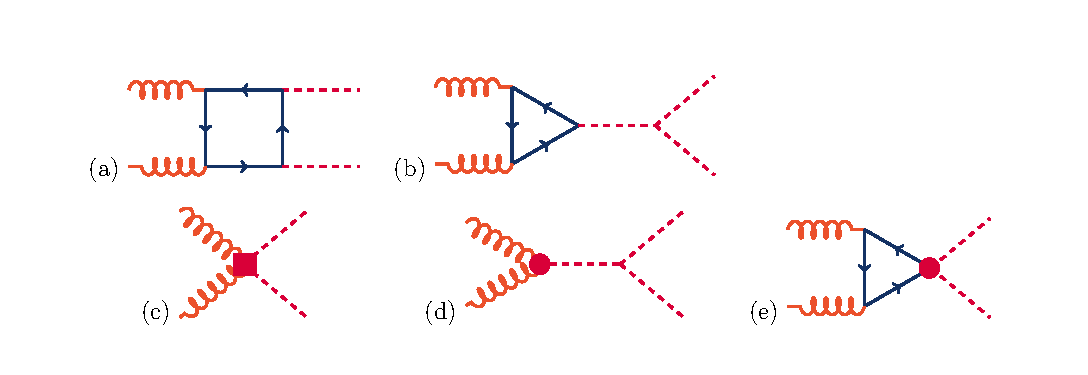
\includegraphics[scale=0.85]{figures/translation.pdf}
\caption{\small Feynman diagrams that contribute to Higgs boson pair production by gluon-gluon fusion at leading order. Diagrams (a) and (b) correspond to SM-like processes, while diagrams (c), (d), and (e) correspond to pure BSM effects: (c) and (d) describe contact interactions between the Higgs boson and gluons, and (e) exploits the contact interaction of two Higgs bosons with top quarks.   \label{fig:dia}}
\end{figure} 

In the Ref.~\cite{Dall'Osso:2015aia} it was designed a method to partition the 5 dimensional parameter space in regions 
with similar LO kinematics. 
When the simulation was launched in the CMS system this work was in preliminary version, we had simulated the samples 
referent to the recommendations of its first version. The list of relevant parameters iused in each sample is in table~\ref{tab:bench}. 
 The {\tt MG5\_aMC@NLO} configuration cards used for the simulations are organized here~\cite{cards}. 
Since then, the metric used by the method was improved and the parameter space scan extended, resulting in a 
new set of benchmarks, that can be found in the last ArXiV version of the mentioned paper, and as well in~\cite{MelladoGarcia:2150771}.


The full simulated samples can be found on DAS as:
\begin{itemize}
  \item \verb|/GluGluToHHTo2B2G_node_X_13TeV-madgraph|
\end{itemize}
where the $X$ ranges between 0 and 13. The $X=0$ represents the point ($\kappa_{\lambda}$, $\kappa_{t}$, $c_2$, $c_g$, $c_{2g}$) = (0,1,0,0,0) - when the process is induced only by the box diagram and the reminiscent correspond to the points listed in Tab.~\ref{tab:bench}.
The analytical formula that allows us to calculate cross sections for any point of the parameter space can be found here~\cite{CarvalhoAntunesDeOliveira:2130724}, and a handful script that calculates the cross sections point by point can be found here~\cite{hhrosetta}.  

%In Figure XX we show the Distributions at Gen level {\bf CHECK}.
In the next session we explain how we had derived results in different benchmark points, based in the above full-simulated samples. \\


\begin{table}
\centering
\small{
\begin{tabular}{|c||c|c|c|c|c|}
\hline
Node & $\kappa_{\lambda}$ & $\kappa_{t}$ & $c_2$ & $c_g$ & $c_{2g}$ \\\hline
1  &   1.0 & 1.0  &  0.0 &  0.0 &  0.0  \\ \hline
2  &   7.5 & 2.5  & -0.5 &  0.0    &  0.0      \\ \hline
3  &  15.0 & 1.5  & -3.0 & -0.0816 &  0.3010   \\\hline
4  &   5.0 & 2.25 &  3.0 &  0.0    &  0.0     \\\hline
5  &  10.0 & 1.5  & -1.0 & -0.0956 &  0.1240  \\ \hline
6  &   1.0 & 0.5  &  4.0 & -1.0    & -0.3780  \\ \hline
7  &   2.4 & 1.25 &  2.0 & -0.2560 & -0.1480  \\ \hline
8  &   7.5 & 2.0  &  0.5 &  0.0    &  0.0     \\ \hline
9  &  10.0 & 2.25 &  2.0 & -0.2130 & -0.0893  \\ \hline
10 &  15.0 & 0.5  &  1.0 & -0.0743 & -0.0668  \\ \hline
11 & -15.0 & 2.0  &  6.0 & -0.1680 & -0.5180  \\ \hline
12 &   2.4 & 2.25 &  2.0 & -0.0616 & -0.1200   \\ \hline
13 & -15.0 & 1.25 &  6.0 & -0.0467 & -0.5150   \\ \hline
\end{tabular}
}
\caption{\small Parameter values of the final benchmarks selected with $N_{clus} = 13$. 
The first cluster is the one that contains the SM sample. 
\label{tab:bench_old}}
\end{table} 

\mbox{}\\{\bf - Distributions at Gen level}

\subsubsection{Reweighting}
\label{sec:rewei}

We are considering a $2\to 2$ process at leading order. The two Higgs bosons are produced with identical transverse momenta ($p_{T}^{H}$), and they are back-to-back in azimuth at this order (before a parton shower). The final state can then be completely defined by three kinematic variables, if we ignore the irrelevant azimuthal angle of emission of the bosons. Furthermore, one of the three remaining variables can be used to isolate all the information related to the PDF of the colliding partons, which is also irrelevant to the physics of the production process once one focuses on a specific initial state (the gluon-gluon fusion process). The variable factorizing out the PDF modeling can be taken as the magnitude of the boost of the centre of mass frame as seen in the laboratory frame. 

The two remaining variables, which provide direct information on the physics of GF HH production, can be chosen to be the invariant mass of the HH system ($m_{HH}$) and the modulus of the cosine of the  polar angle of one Higgs boson with respect to the beam axis ($|cos\theta^*|$). Since we are using parton-level information, this last variable is equivalent to the polar angle in the Collins-Soper frame ($|cos\theta^*_{CS}|$)~\cite{PhysRevD.16.2219}, which is commonly used in experimental analysis. The variables $m_{HH}$ and $|cos\theta^*|$ can thus be used to fully characterize the final state kinematics produced by different choices of the value of anomalous Higgs boson (self-) coupling parameters.

By construction the full-simulated samples listed in Tab.~\ref{tab:bench}  are good representatives of the kinematic space. 
Therefore, based in the generation level $m_{HH}$ and $|cos\theta^*|$, those can be used to construct 
samples to any other parameter space point. 

The procedure is made as follows: 
\begin{itemize}
\item For each new parameter space point we perform 
a simulation in {\tt MG5\_aMC@NLO}, asking for $N$ events;
\item We construct two dimensional histograms in the 
generation level $m_{HH}$ and $cos\theta^*$, with 20$\GeV$-wide bins in the $m_{HH}$ and
 0.2-wide bins in $cos\theta^*$ (without the moduli);
\item We construct the same histogram with the sum of all the full simulated samples described in the last section (signal dataset);
\item The new sample is constructed by weigthing the signal dataset event-by-event by:
 \begin{equation}
 W_{e} = \frac{New_{ij}}{D_{ij}}\,,
 \end{equation}
 where ($ij$) specify the bin in which the event $e$ belongs and $New_{ij}$ ($D_{ij}$) the number of events of the 
 new signal sample (signal dataset) in that bin. 
 \end{itemize}
 
 We make reweighted samples for three types of theory scans:
\begin{itemize}
%  \item The frozen list of benchmarks of Refs.~\cite{Dall'Osso:2015aia,MelladoGarcia:2150771}, listed in Tab.~\ref{tab:bench}. 
  \item A plain scan in $\kappa_{\lambda}$, while all the other parameters are kept as in SM ($\kappa_{t}$, $c_2 = c_g  = c_{2g} =0$), where the gen-level histograms are made from 50,000 events
  \item Another set of samples that we will use to calculate the shape systematics necessary to extrapolate the limits in the benchmarks to an extended part of the parameter space (see Sec.~\ref{sec:shapesyst}).
\end{itemize} 
%The 2D histograms to construct the new samples are HERE and the map pf weights to the dataset BLA is HERE.
 
 \begin{table}[h]
\centering
\small{
\begin{tabular}{rccccc}
\hline
Benchmark & $\kappa_{\lambda}$ & $\kappa_{t}$ & $c_{2}$	& $c_{g}$ & $c_{2g}$ \\\hline
1 &	7.5	 & 1.0	 &	-1.0	& 0.0	& 0.0 \\
2 &	1.0	 & 1.0	 &	0.5		& -0.8	& 0.6 \\
3 &	1.0	 & 1.0	 &	-1.5	& 0.0	& -0.8 \\
4 &	-3.5 & 1.5  &	-3.0	& 0.0	& 0.0 \\
5 &	1.0	 & 1.0	 &	0.0		& 0.8	& -1 \\
6 &	2.4	 & 1.0	 &	0.0		& 0.2	& -0.2 \\
7 &	5.0	 & 1.0	 &	0.0		& 0.2	& -0.2 \\
8 &	15.0 & 1.0	 &	0.0		& -1	& 1 \\
9 &	1.0	 & 1.0	 &	1.0		& -0.6	& 0.6 \\
10 &	10.0 & 1.5   &	-1.0	& 0.0	& 0.0 \\
11 &	2.4	 & 1.0	 &	0.0		& 1		& -1 \\
12 &	15.0 & 1.0	 &	1.0		& 0.0	& 0.0 \\ \hline %cl no. 463
SM &	1.0 & 1.0	 &	0.0		& 0.0	& 0.0 \\
\hline
\end{tabular}
}
\caption{\small Parameter values of the twelve benchmarks and the Standard Model point.  \label{tab:bench}}
\end{table}
 
\subsubsection{Non-resonant Vector Boson Fusion}

For the 2016 version of the analysis, one non-resonant VBF sample was also produced centrally with the Standard Model coupling parameters. 
The MiniAOD version of this sample can be found on DAS under:   
/VBFHHTo2B2G\_CV\_1\_C2V\_1\_C3\_1\_13TeV-madgraph/RunIISummer16MiniAODv2-PUMoriond17\_80X\_mcRun2\_asymptotic\_2016\_TrancheIV\_v6-v1/MINIAODSIM
 
\subsection{Background MC}

Even though the signal extraction and background modeling of this analysis are performed based on data, background Monte Carlo samples are used to validate the simulation of our signal description and to develop the analysis. The main backgrounds for the $\bbgg$ final state come from either well-isolated photons coming from the hard scatter (prompt photons) or isolated photons reconstructed due to very collimated $\pi^{0}\to\gamma\gamma$ decays fragmented from jets (fake photons). These backgrounds are the same as the ones to the SM $\Hgg$ analysis, and a more complete description of the samples used can be found in the $\Hgg$ AN ~\cite{Hgg2015, Hgg2016}.

We can classify these backgrounds with respect to the number of prompt and fake photons in the selected diphoton candidate. The prompt-prompt background events are simulated with the Sherpa generator; it includes the born processes with up to 3 additional jets at LO accuracy as well as the box processes at LO. The prompt-fake and the fake-fake contributions are simulated with PYTHIA8, with a "Double-EM Enriched" filter\footnote{it requires a high $\pt$ and well isolated photon-like signal (electromagnetic activity) coming from photons, electrons, or neutral hadrons)} applied during production to improve the samples selection efficiencies. Additionally, a sample of Drell-Yan events decaying into electrons, simulated at NLO with AMC@NLO, is used, although its final contribution to the event yield is minimal due to the $M(\gamma\gamma) > 100 \gev$ selection cut.

\subsection{Data}

The data samples used in this analysis correspond to approximately $36.5$ fb$^{-1}$ of data collected in 2016, reconstructed with the 80X CMSSW release.



\clearpage
\section{Analysis objects and selection}
This analysis uses general purpose reconstruction of the photons and jets for which we
have brief descriptions below.
\section{Analysis objects and selection}
This analysis uses general purpose reconstruction of photons and jets, which have been described in previous sections. 
We have brief descriptions below, pointing out specific choices made for the analysis.

\subsection{Triggers And Pre-Selection}
\label{sec:trigger}
Exploiting the high online performance of the CMS ECAL to reconstruct photons and electrons, the dataset used in this analysis is constructed with a selection that requires two photons at High Level Trigger (HLT) level.

For the 2016 data taking period, the online strategy was based on a single HLT trigger path:
\begin{itemize}
\item HLT$\_$Diphoton30$\_$18$\_$R9Id$\_$OR$\_$IsoCaloId$\_$AND$\_$HE$\_$R9Id$\_$Mass90;
\end{itemize}

In order to achieve a good data/simulation comparison, a pre-selection that is tighter than the online selection is applied on data and Monte Carlo. This pre-selection is described on table \ref{tab:preselection}. It is based on shower shape variables ($R9$, the ratio between the energy deposited on a 3x3 ECAL crystal matrix around the most energetic crystal in the supercluster, and the supercluster energy), isolation variables (charged hadron isolation, CHI, the sum of all charged hadron particle flow candidates energies inside a cone of $\Delta R < 0.3$ around the photon axis), identification variables (H/E, the ratio between the photon's energy deposit on HCAL and on ECAL), and kinematic variables ($E_{T}$ and the photon supercluster $\eta$). Only events that have at least one diphoton candidate passing the pre-selection requirements are considered in the analysis.

 \begin{table}[h]
\centering
\small{
\begin{tabular}{rcc}
Requirements & Leading Photon & Subleading Photon \\ \hline
$E_{T}$ & $30 \gev$ & $20 \gev$ \\ \hline
$|\eta|$ & \multicolumn{2}{c}{ $< 2.5$ and outside $1.442  |\eta| < 1.566$ } \\ \hline
Shower shape and Isolation & \multicolumn{2}{c}{ $R9 > 0.8$ or CHI $< 20$ or CHI/$E_{T} < 0.3$} \\ \hline
Identification & \multicolumn{2}{c}{ H/E $< 0.08$} \\ \hline
\end{tabular}
}
\caption{\small Trigger based pre-selection applied on diphoton candidates.  \label{tab:preselection}}
\end{table}

The SM $\Hgg$ analysis provides scale factors and uncertainties related to those scale factors due to this HLT selection, which we also apply in the analysis and take into account in our final list of systematics. 

\clearpage
\subsection{Photons}
\label{sec:photons}

The kinematic requirements applied on the photons, after the diphoton candidates have passed through the event pre-selection (see Section ~\ref{sec:trigger}), are similar to the ones used in the SM $\Hgg$ analysis. The selection is as follows:
\begin{itemize}
\item Leading photon $E_{T} > 30 \GeV$, trailing photon $E_{T}>20 \GeV$;
\item Leading photon $E_{T}/\Mgg > 1/3$, trailing photon $E_{T}/\Mgg > 1/4$;
\item $100 < \Mgg < 180 \GeV$.
\end{itemize}
Additionally, a photon identification requirement is applied to the photons.

The photon identification requirement is based on a multivariate algorithm that combines information from the photon cluster shape in ECAL, as well as isolation variables. 
This requirement provides a signal-like photon efficiency of $90\%$ for photons both on the ECAL barrel and endcaps. 
The scale factors used to ensure data/MC agreement in the selection efficiency are also applied; these scale factors are calculated centrally at CMS. 
Additionally, an electron veto is applied to avoid background with electrons faking photons, with corresponding scale factors and uncertainties.

%=========== OLD ===========

%Currently (as of January 2016), the available samples processed by the $\Hgg$ group only have stored 
%their own training of the photon MVA ID. 
%We have chosen working points that ensure that the resonant low mass samples have 
%a $90\%$ efficiency both in the barrel and the endcap ECAL regions. 

%\begin{table}[h]
%\centering
%\begin{tabular} { | c | c | }
%\hline
%ECAL Region & Hgg MVA Selection \\ \hline
%EB & 0.07 \\ \hline
%EE & -0.03 \\ \hline
%\end{tabular}
%\end{table}

%Efficiencies of the leading photon to pass the ID criteria, as a function of the photon transverse energy, 
%are shown in Figure \ref{fig:Hgg-PhoID-eff}. 
%Only photons matched to gen-level prompt photons are used. 


%\begin{figure*}[thb]
%  \centering
%  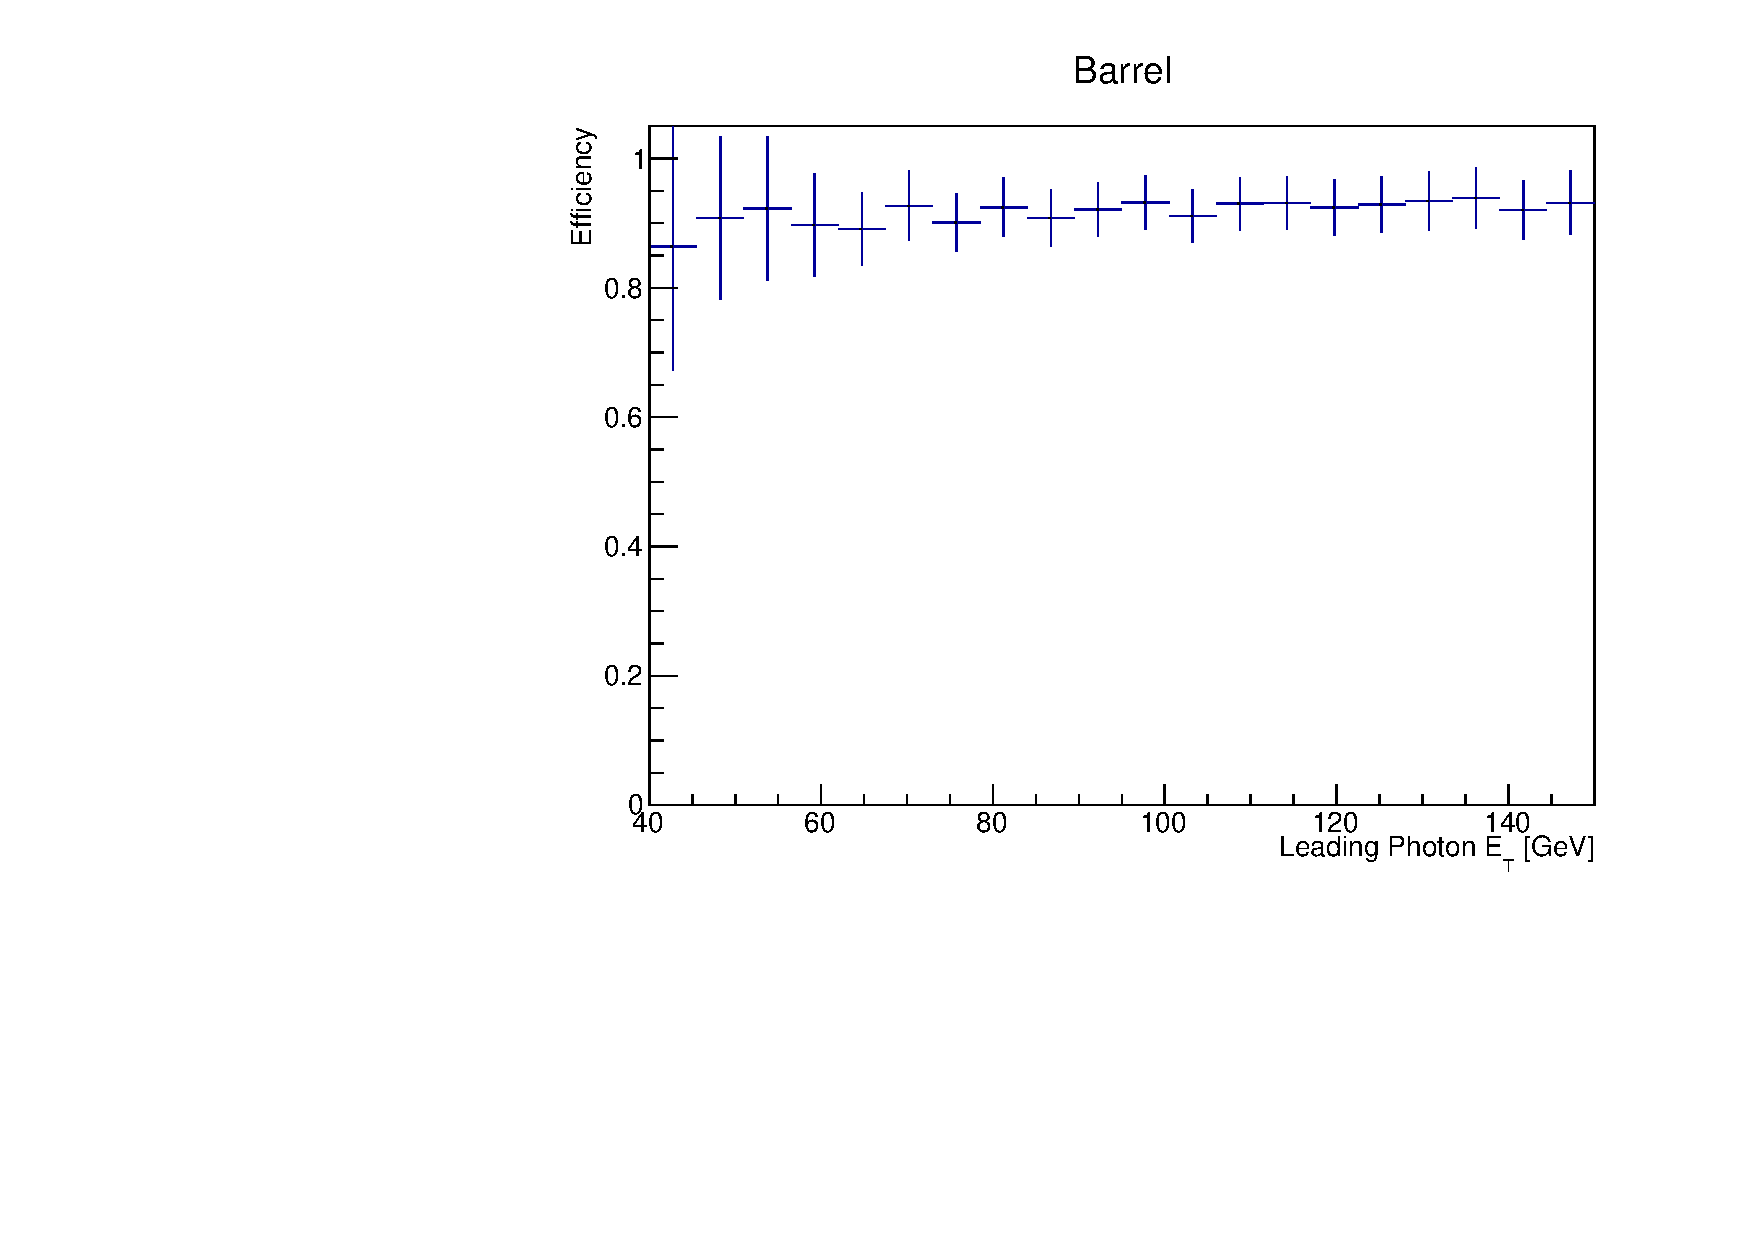
\includegraphics[width=0.45\textwidth]{figures/sec-photons/SMHH_HggMVA_Eff_EB.pdf}\hfil
%  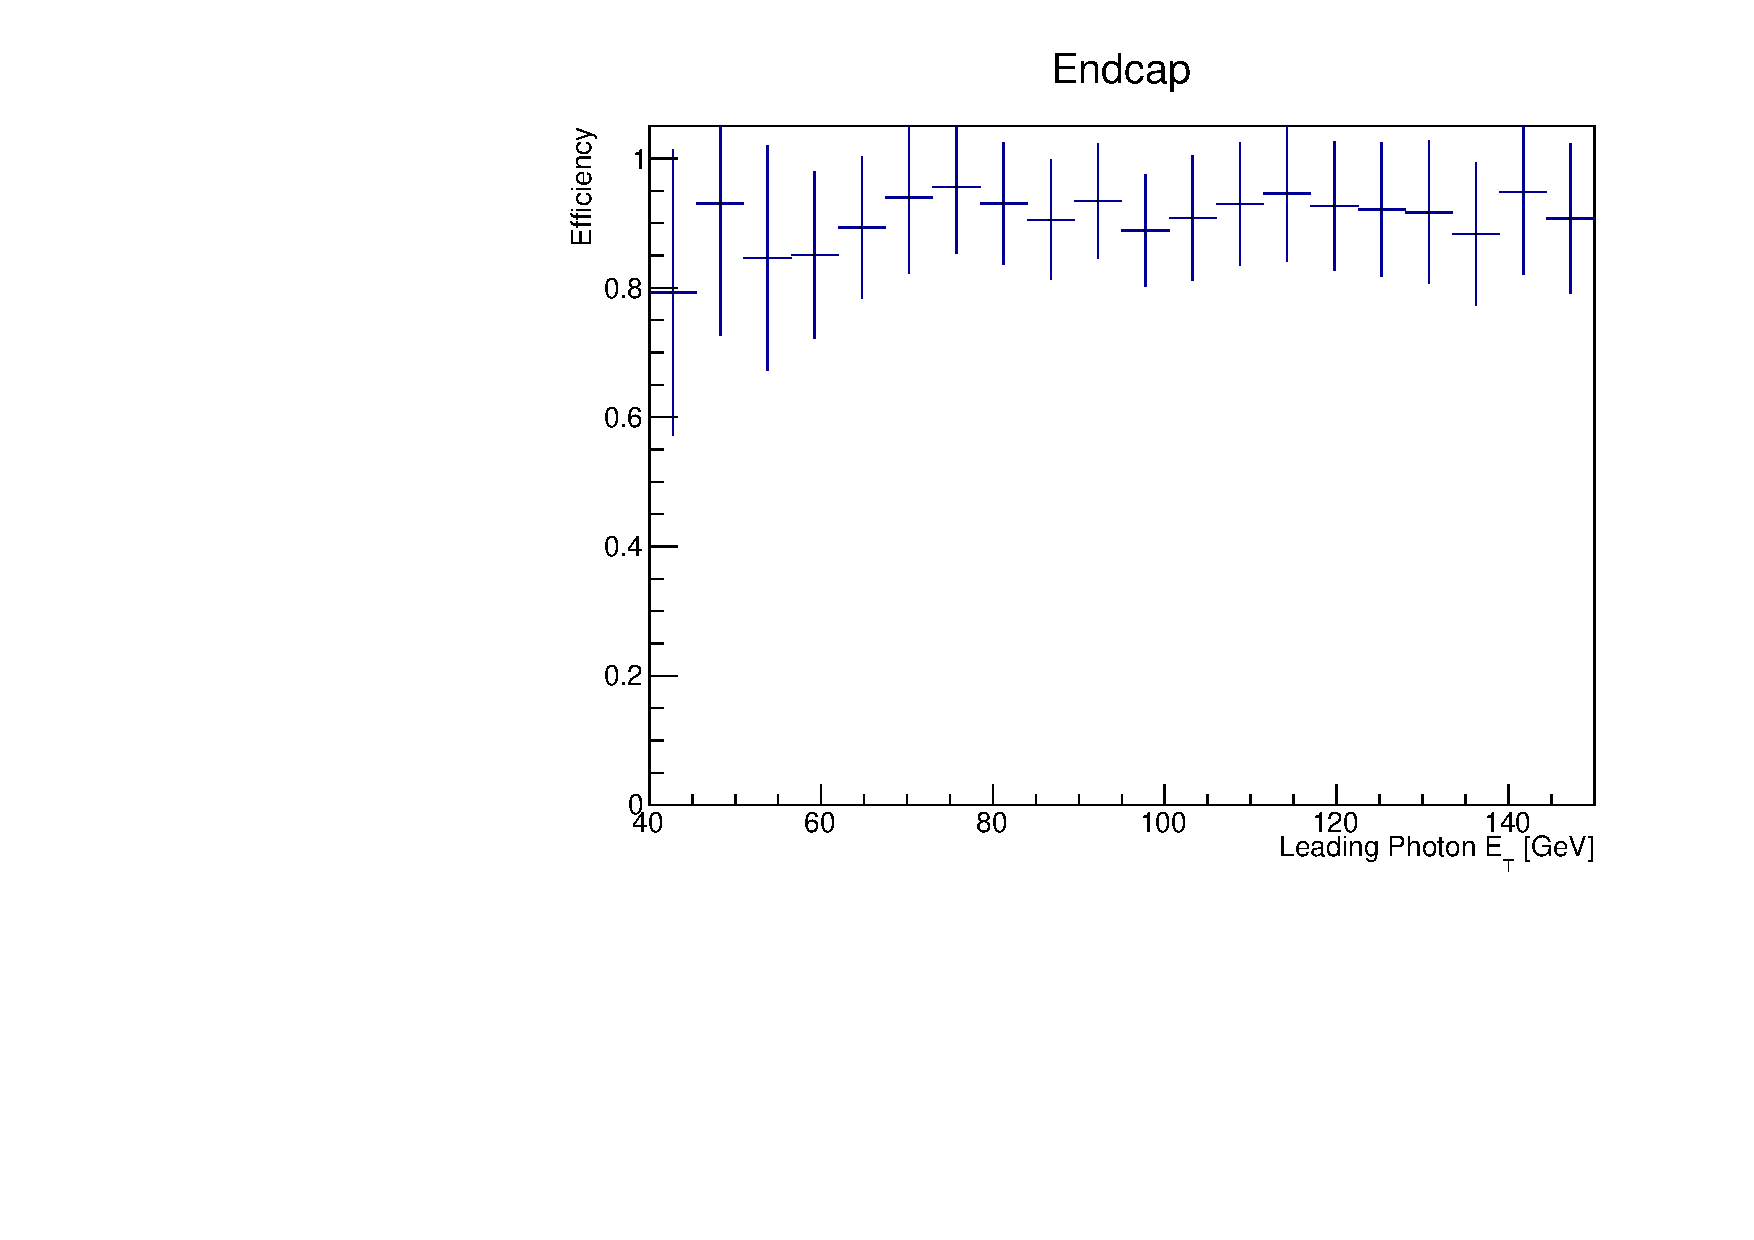
\includegraphics[width=0.45\textwidth]{figures/sec-photons/SMHH_HggMVA_Eff_EE.pdf}\hfil
%  \caption{Efficiencies of the leading photon to pass the ID criteria, as a function of the photon transverse energy, 
%for photons in the barrel and endcap regions of ECAL. }
%  \label{fig:Hgg-PhoID-eff}
%\end{figure*}

%We have studied all of those possibilities with MC samples, and for the 2015 data we
%decided to use the MVA ID of EGamma group with \textit{Loose} working point (WP),
%corresponding to 90\% signal selection efficiency.  A brief summary of this study is
%described below.

%The true photons are selected from the $G \to \HH \to \bbgg$ signal MC samples (they are
%required to match the generated level photons within $\Delta R< 0.1$ cone). The fake
%photons are selected from the Double-EM enriched $\gamma$+jet samples (and they must not
%to match to any generated level photon).
%The studied photons must pass the standard photon selection (pre-selection plus kinematic selection).

%Finally, the MVA score is calculated for the selected photons (or an ID decision for the
%cut-based ID).  Figure \ref{fig:phoID-MVA} shows two examples of the MVA output from the
%signal and fake photons. And Figure~\ref{fig:phoID-ROC} shows the ROC curves for the three
%IDs considered, for photons in the Barrel and Endcap. On these curves at a given signal
%efficiency one would prefer to have highest background rejection. From this figure of
%merit the MVA IDs are undoubtedly better than the cut-based ID. While the two MVA IDs have
%very similar performance.

%Note: it is anticipated that for 2016 data-taking the two MVA IDs will merge into one, and we
%will use that.

%\begin{figure*}[thb]
%  \centering
%  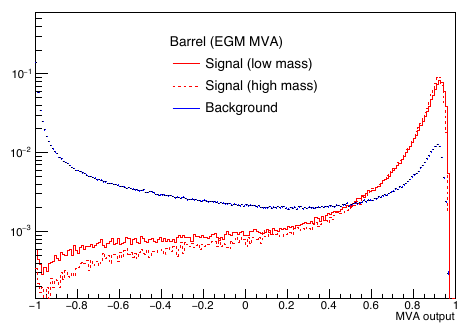
\includegraphics[width=0.45\textwidth]{MVA_output_EGM_Barrel}\hfil
%  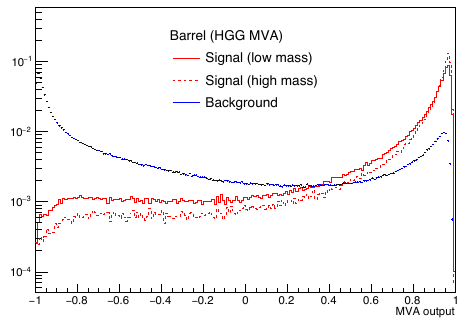
\includegraphics[width=0.45\textwidth]{MVA_output_HGG_Barrel}\hfil
%  \caption{Examples of the MVA ID outputs for the photons in the Barrel. Left: EGamma,
%    right: Hgg.}
%  \label{fig:phoID-MVA}
%\end{figure*}


%\begin{figure*}[thb]
%  \centering
%  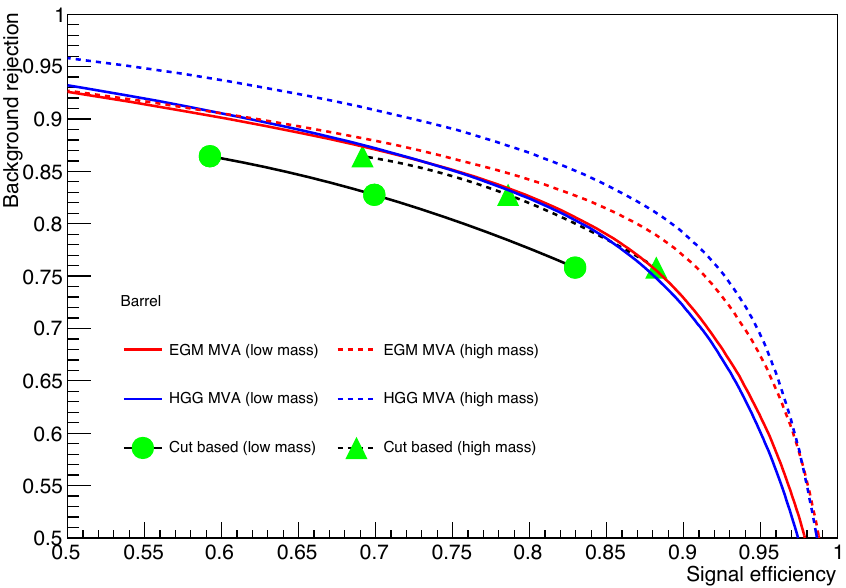
\includegraphics[width=0.45\textwidth]{ming_phoID_EB}\hfil
%  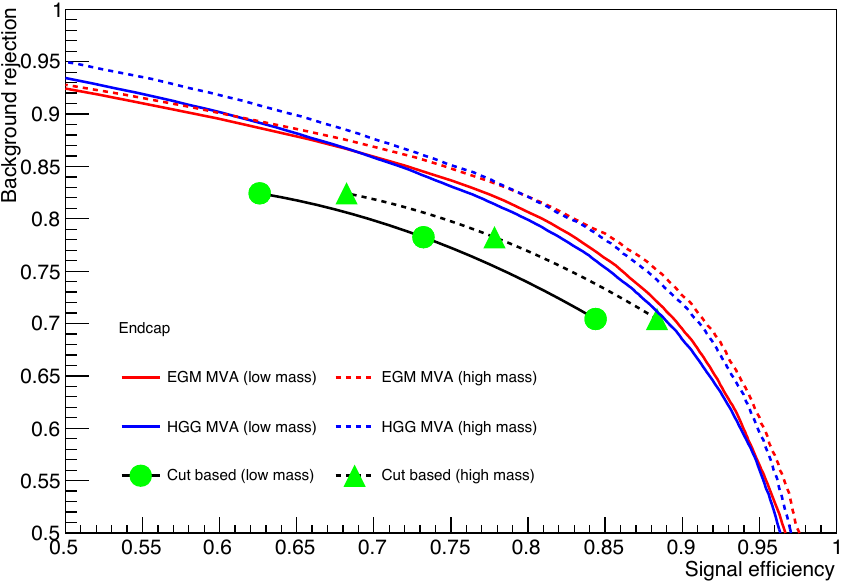
\includegraphics[width=0.45\textwidth]{ming_phoID_EE}\hfil
%  \caption{Photon ID ROC curves}
%  \label{fig:phoID-ROC}
%\end{figure*}

\subsubsection{Fake Photon Control Region}\label{sec:PCR}
A control region is created by selecting diphoton candidates with one photon that passed the ID requirement and one that didn't. All the other selections remain the same, and the procedure to select such diphoton candidates is the same as in the signal region. This control region is used in the analysis to perform closure tests on the background modeling.

\subsubsection{Vertex}
Inheriting from the main $\Hgg$ analysis, we use the vertex that gives the highest $\Hgg$ vertex MVA score. 
Because there are additional jets in the event,  picking this vertex has a very small mismatch efficiency. 
Only in less than $0.1\%$ of the events, the chosen vertex is different from the vertex associated to the true vertex in the simulation. 

The $\Hgg$ vertex MVA score is based on three variables calculated for each reconstructed vertex: the sum of the squared transverse momenta of the charged particle tracks associated with the vertex, and two variables that quantify the vector and scalar balance of $p_{T}$ between the diphoton system and the charged particle tracks associated with the vertex. 
In addition, if either photon is associated with any charged particle track that has been identified as resulting from conversion, the conversion information is also used. 
The variables are used as the inputs to a multivariate classifier based on a boosted decision tree (BDT) to choose the reconstructed vertex to be associated with the diphoton system. 
The average vertex finding efficiency of this algorithm in the SM $\Hgg$ analysis is $80\%$.

\subsubsection{Gain Switch}

In 2016, it was observed that high energy deposits in ECAL had their energies reconstructed with a certain bias, due to the shaping of the pulses in the ECAL VFE electronics. 
This shaping became a problem in Run 2 because we assume a certain shape for the signal amplitude from the crystals when measuring this amplitude, as described in the Multifit method. 
It has been observed that this bias occurs when an energy deposit is high enough to cause a gain switch in the ECAL multi-gain amplifier.

We investigated the fraction of selected events in our blinded signal region with photons that go through gain switches. 
The plots on Figure \ref{fig:gain_switch}  show, in bins of $\tilde{M}_{X}$, the fraction of events with at least one of the photon candidates going through gain switches (to gain 1, gain 6 or both). 
These results show that, for the high mass region, around $20\%$ of our events are affected by gain switches. 
This non-negligible rate means that the analysis needs to use the new CMS re-processed data in which the issue has been fixed.

\begin{figure*}[thb]
  \centering
%  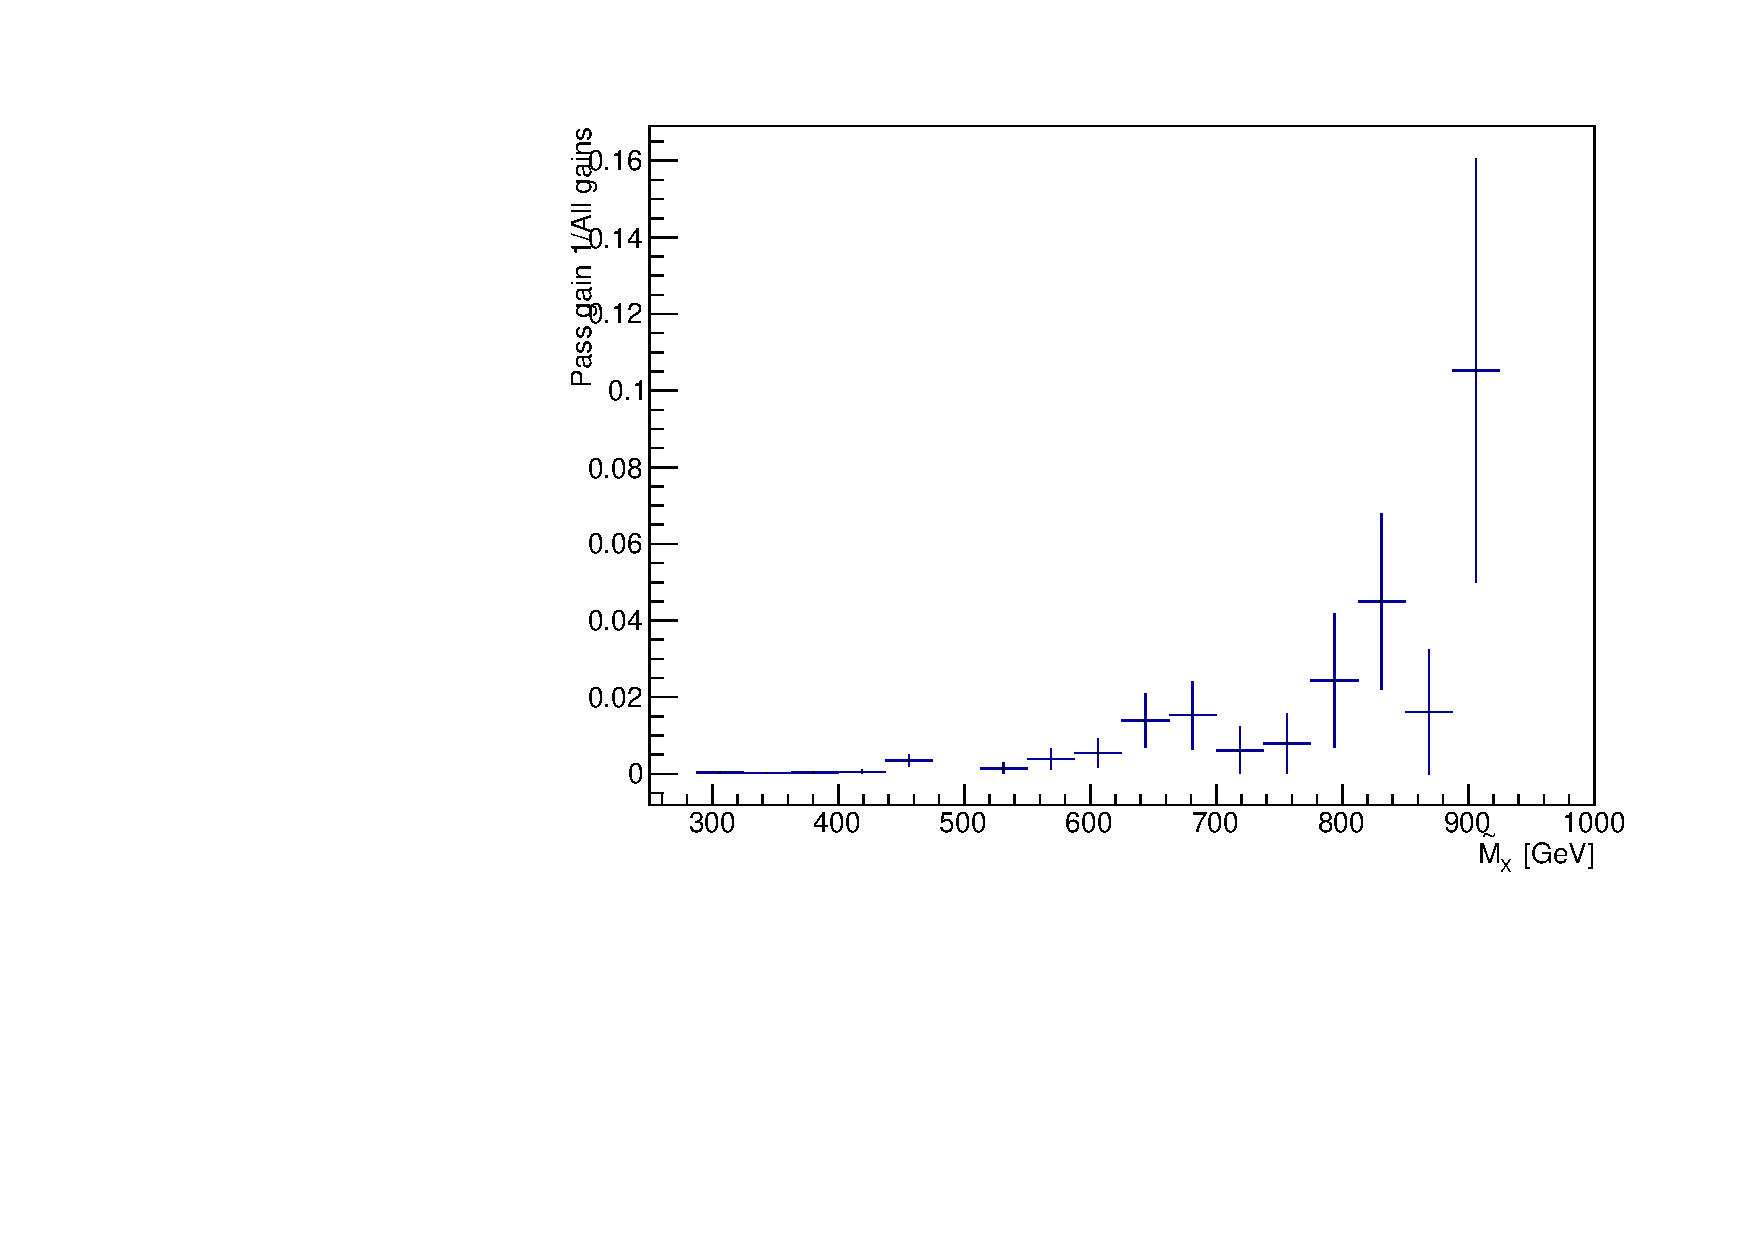
\includegraphics[width=0.3\textwidth]{figures/sec-photons/rg1}\hfil
%  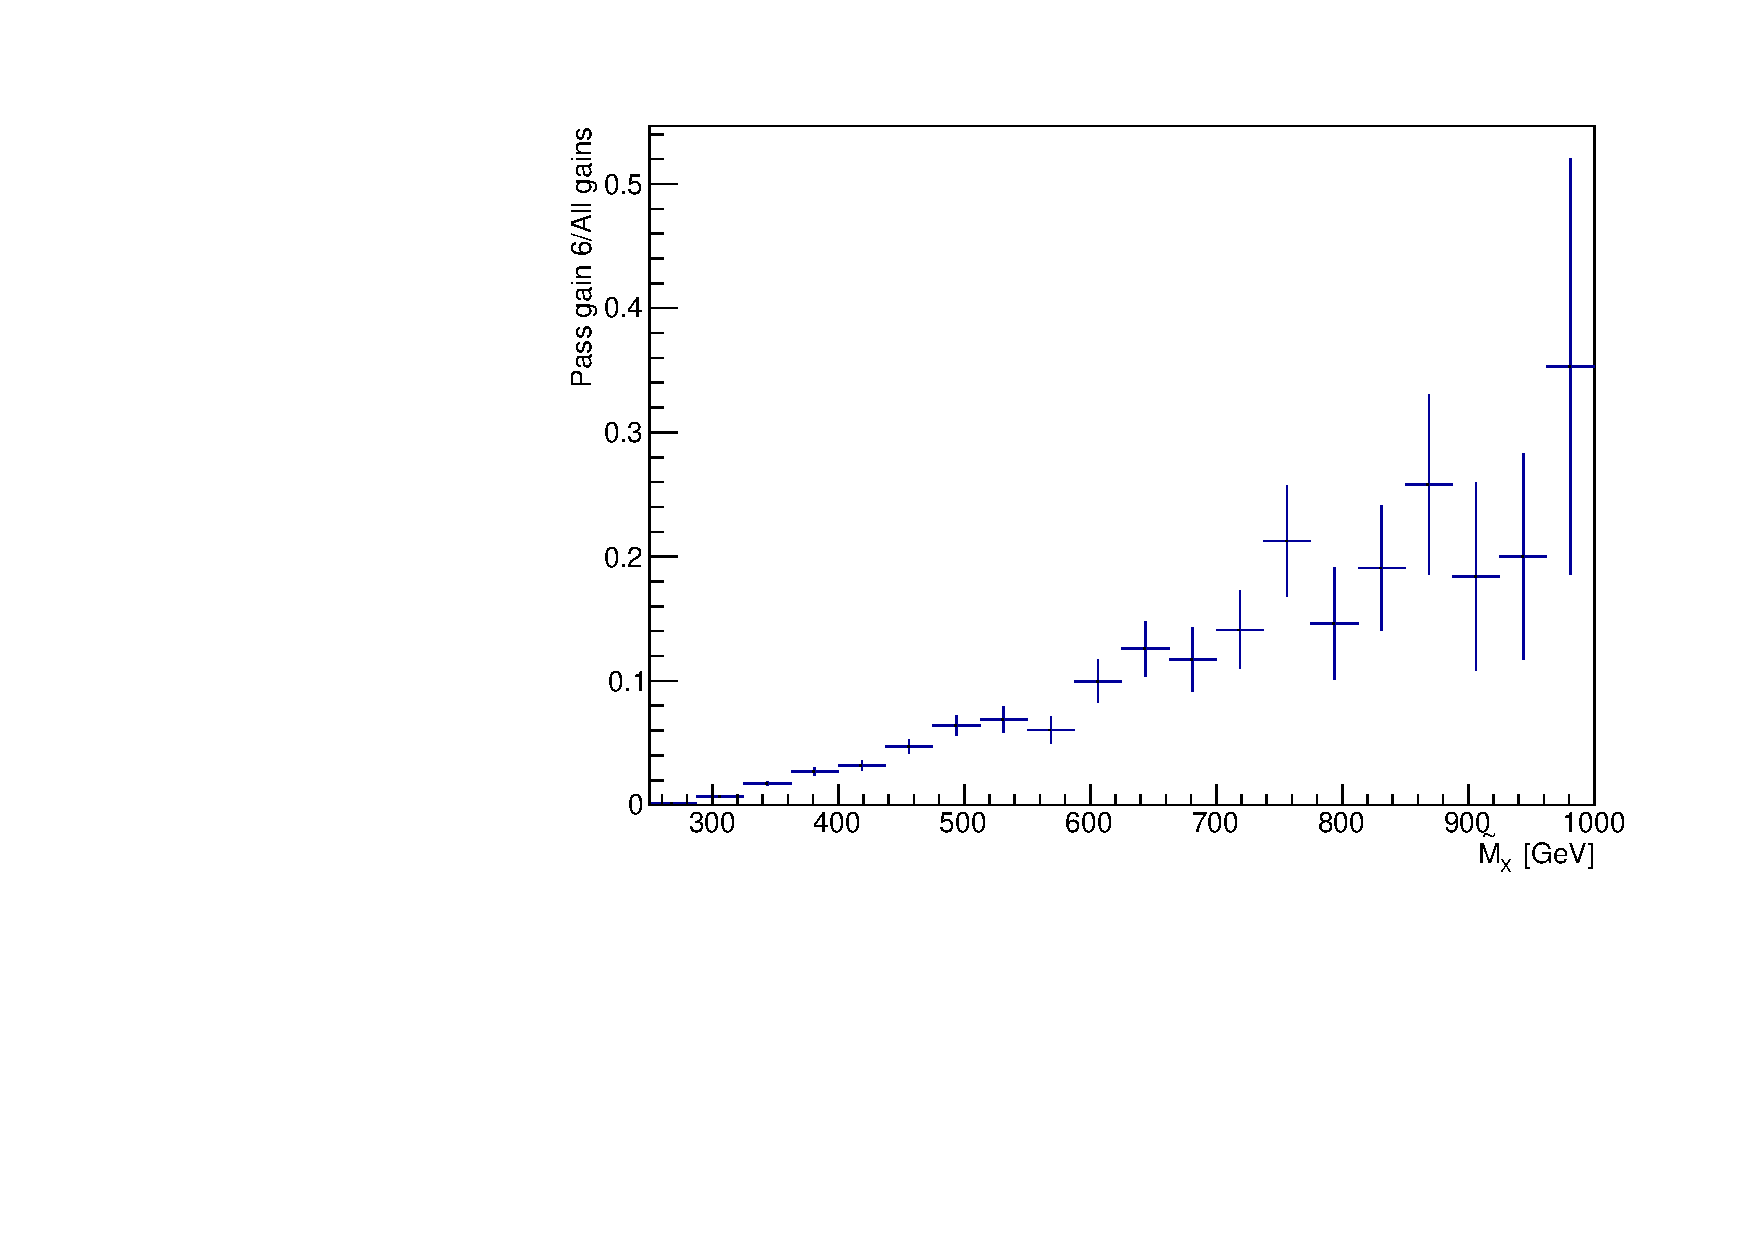
\includegraphics[width=0.3\textwidth]{figures/sec-photons/rg6}\hfil
  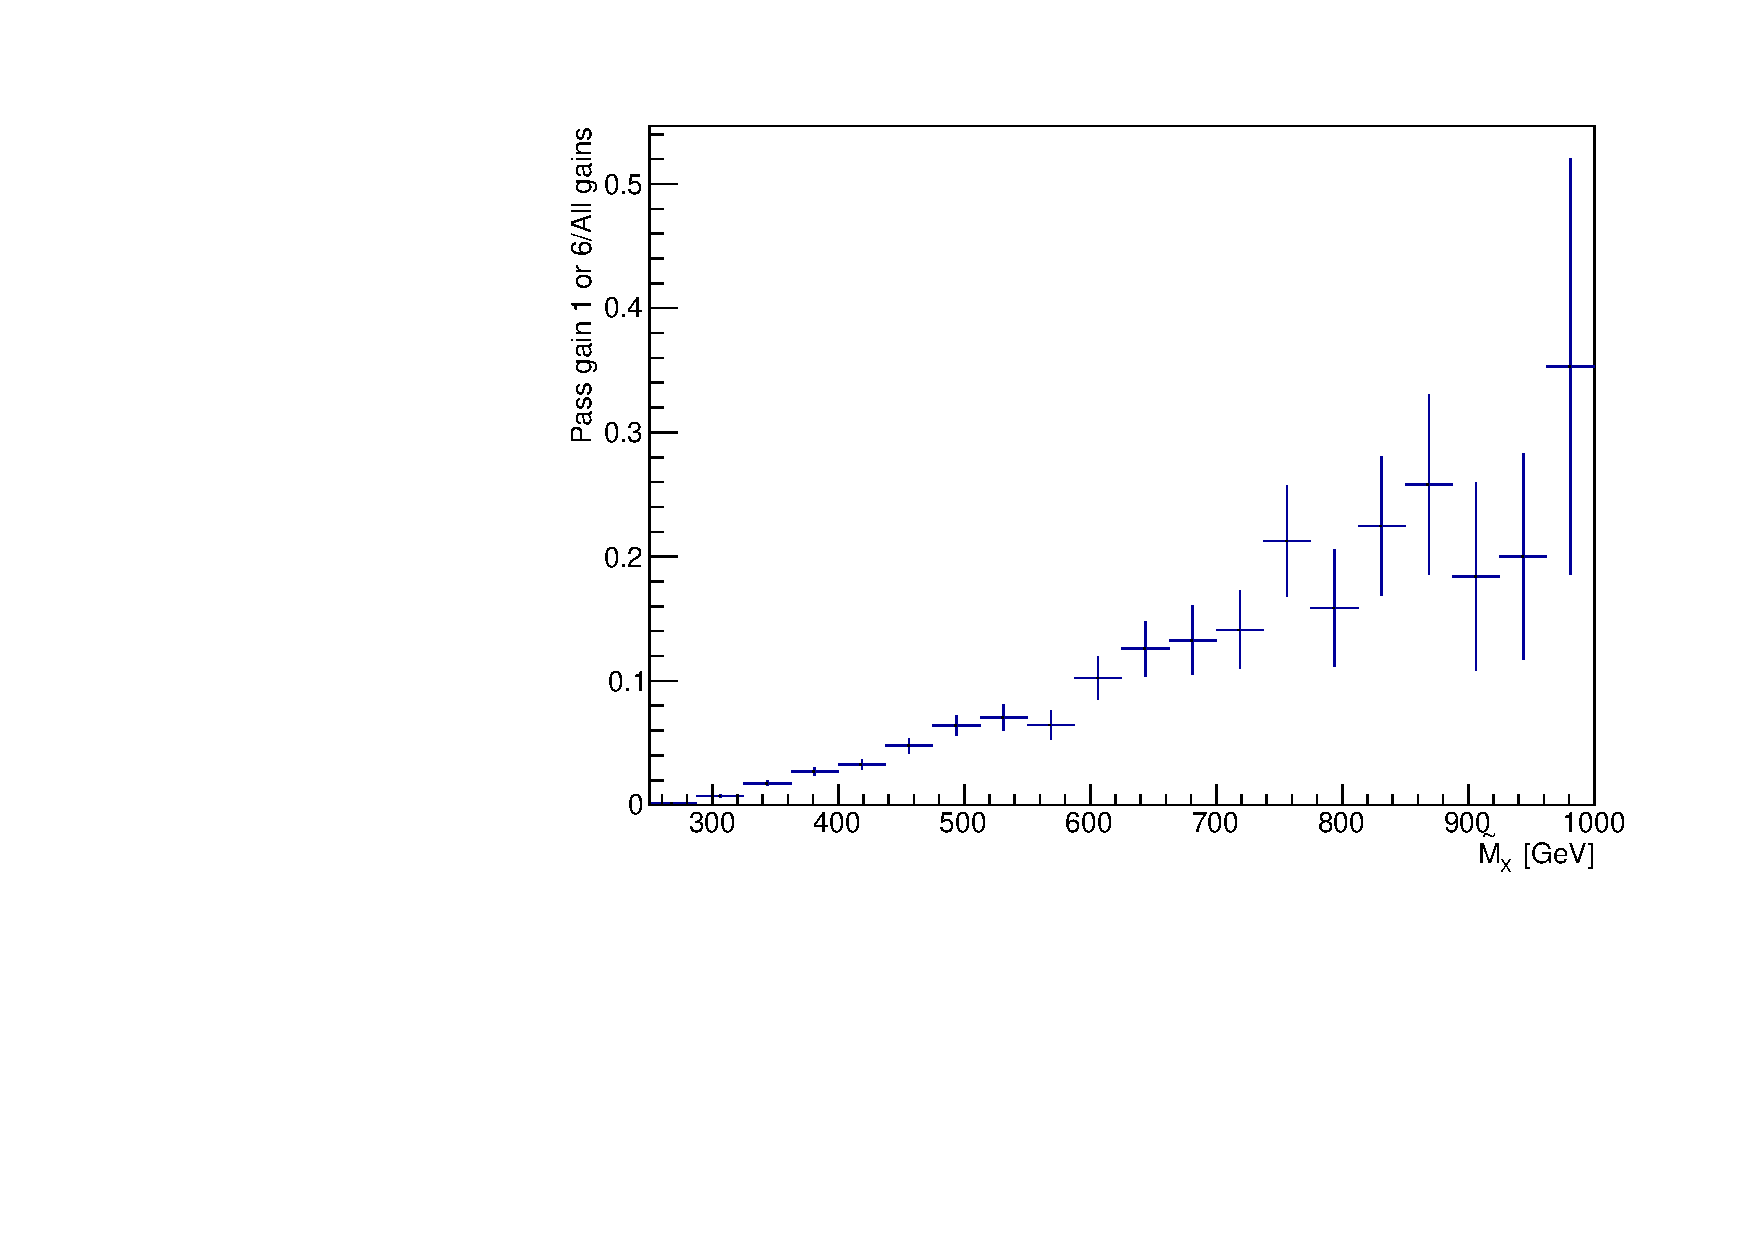
\includegraphics[width=0.5\textwidth]{figures/sec-photons/rg16}
  \caption{Fraction of events with photon candidates going through gain switch.}
  \label{fig:gain_switch}
\end{figure*}

\subsubsection{Regression}

A new version of the photon energy regression has been trained with the Run 2 data taking conditions. 
This regression aims to correct the photon super cluster energy, as described in previous sections.  
We compared this new regression to the previous training, as seen in the plots of Figure \ref{fig:pho_reg} for three different resonance mass points. 
The difference observed is not large enough for this analysis to be affected, so the previous regression version is used (following main $\Hgg$ analysis).

\begin{figure*}[thb]
  \centering
  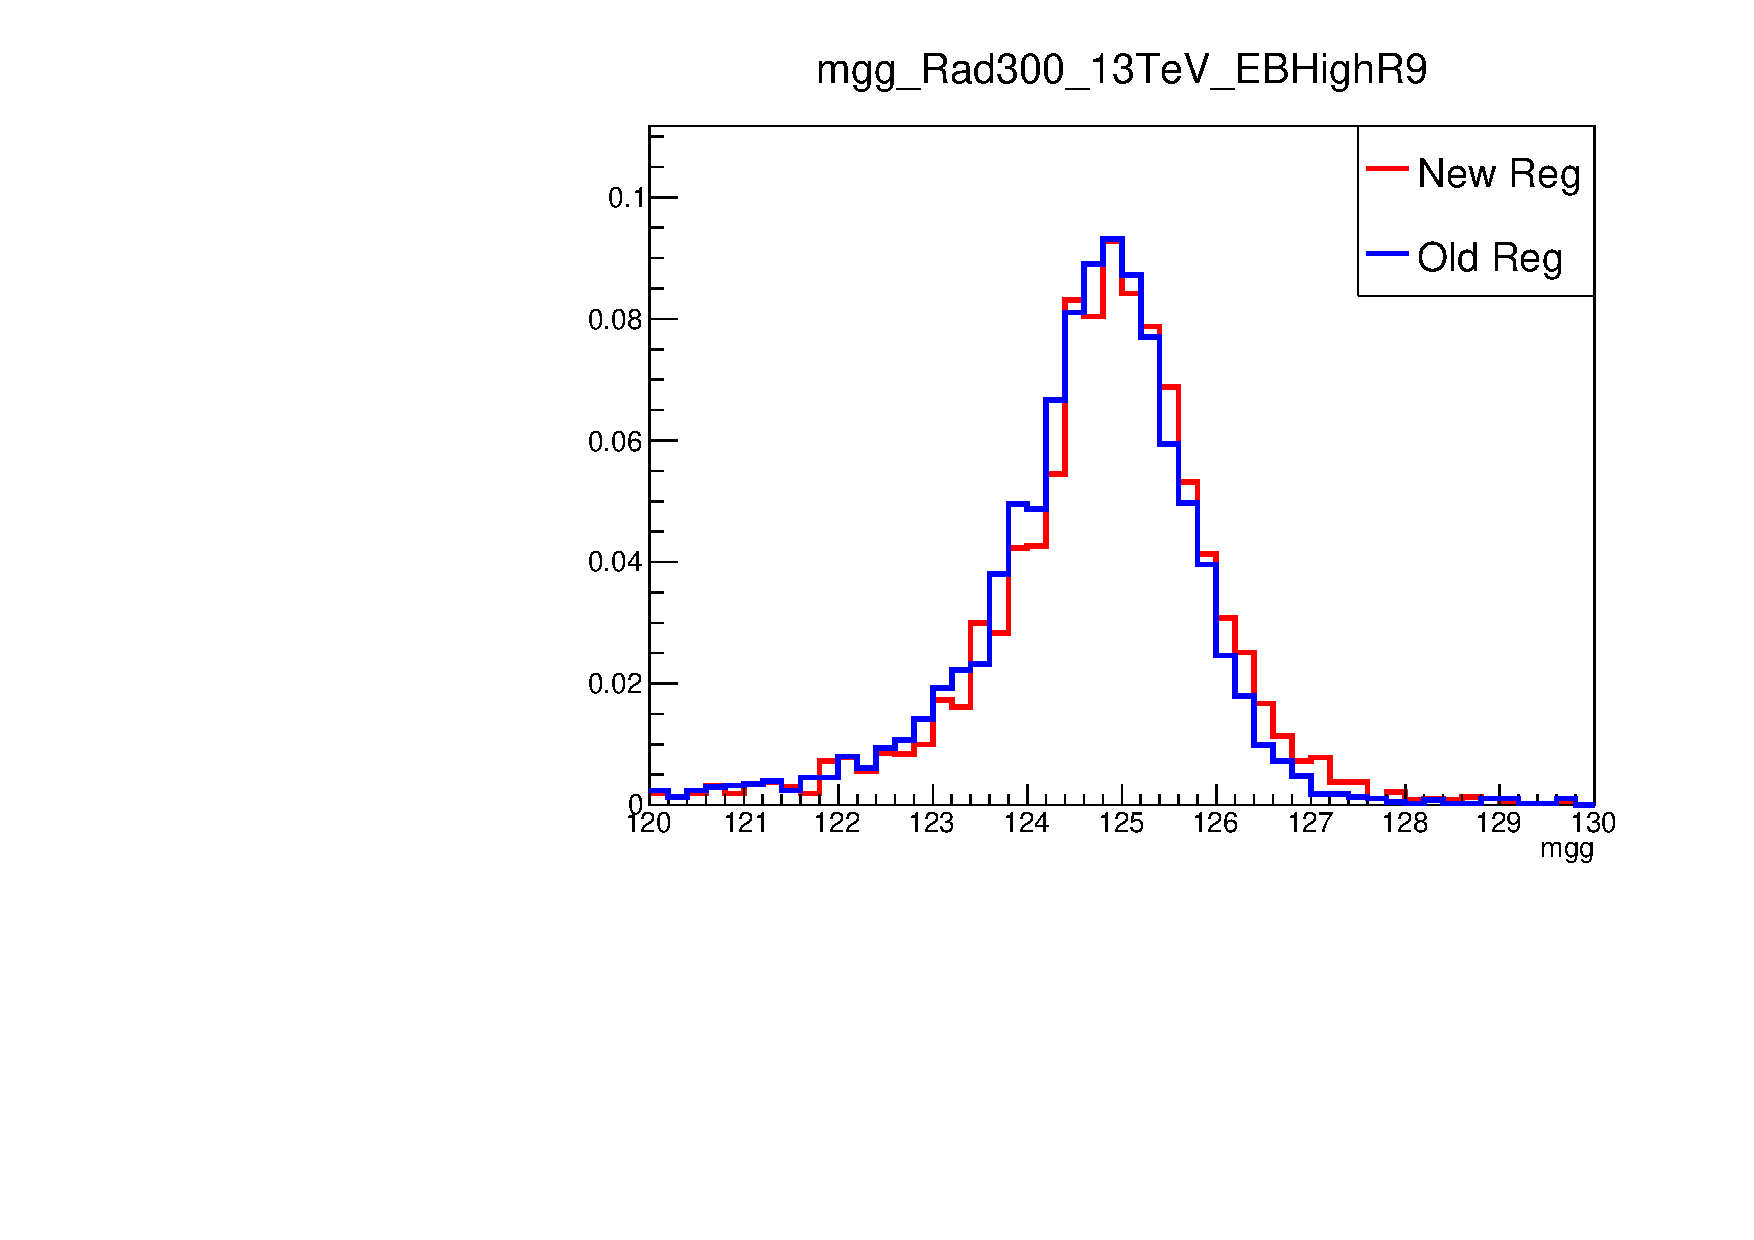
\includegraphics[trim={0 0 0 0.95cm},clip,width=0.3\textwidth]{figures/sec-photons/mgg_Rad300_13TeV_EBHighR9.pdf}\hfil
  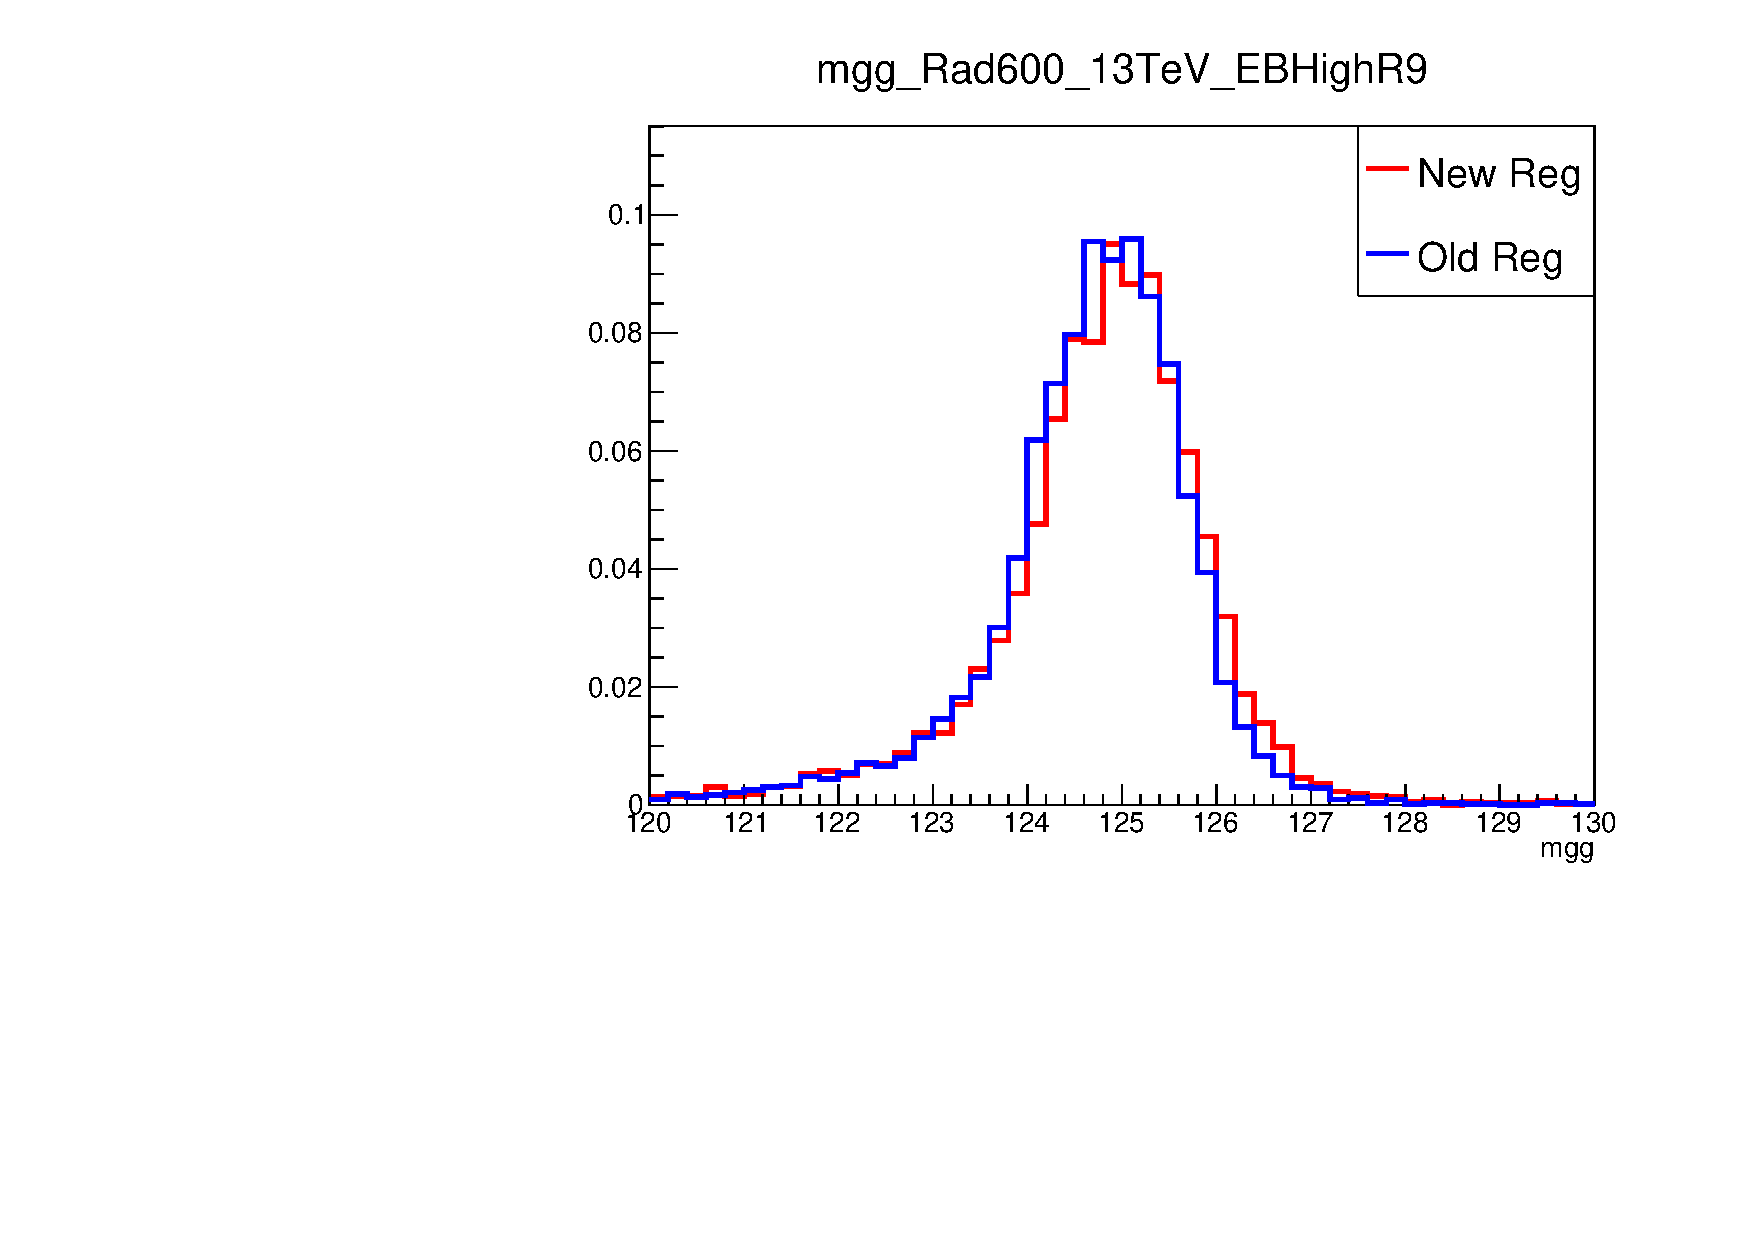
\includegraphics[trim={0 0 0 0.95cm},clip,width=0.3\textwidth]{figures/sec-photons/mgg_Rad600_13TeV_EBHighR9.pdf}\hfil
  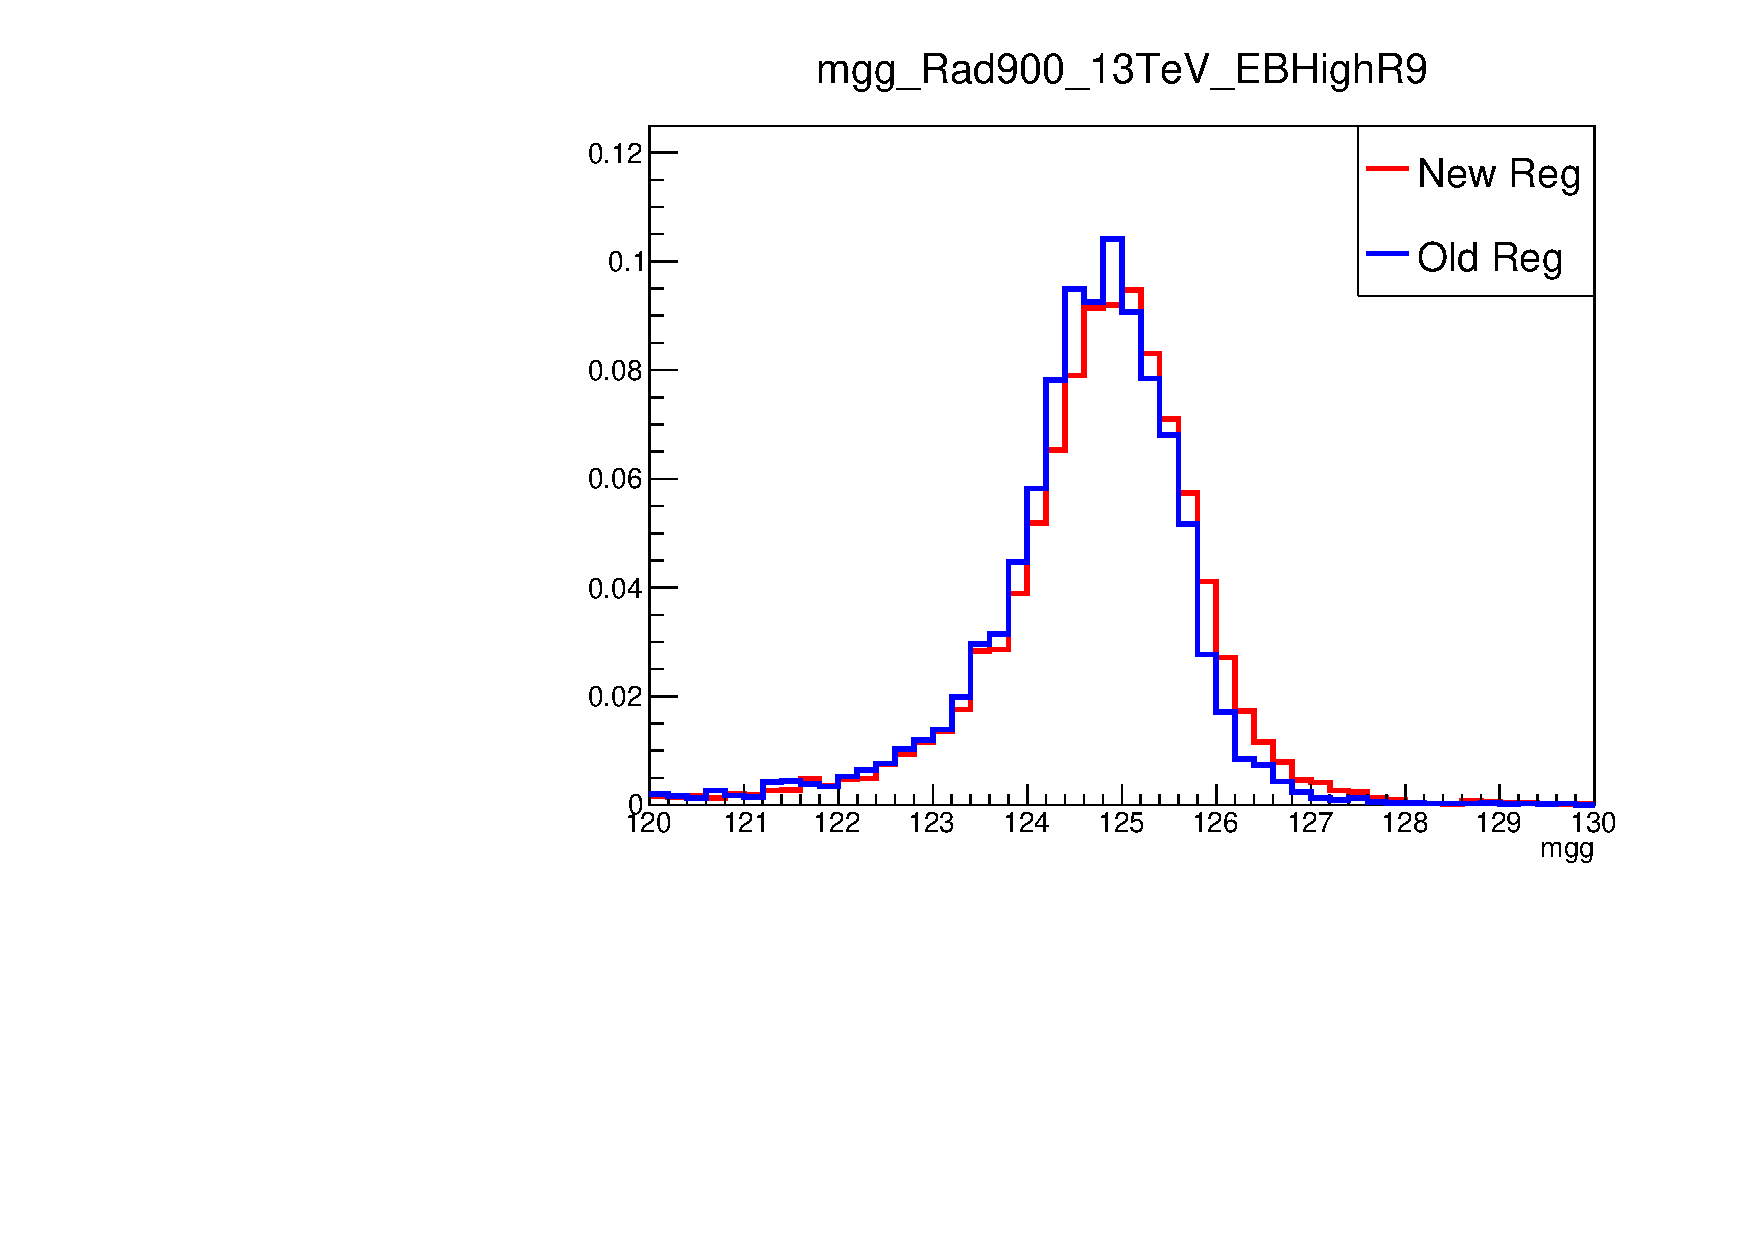
\includegraphics[trim={0 0 0 0.95cm},clip,width=0.3\textwidth]{figures/sec-photons/mgg_Rad900_13TeV_EBHighR9.pdf}\hfil
  \caption{$M(\gamma\gamma)$ reconstructed with different versions of the photon energy regression for resonance masses of 300, 600 and 900 GeV, from left to right. Distributions normalized to unity.}
  \label{fig:pho_reg}
\end{figure*}

\clearpage
\subsection{Jets}
\label{sec:jets}

The jets in Run-II at CMS are reconstructed using anti-kt algorithm
with the distance parameter $R=0.4$. This was a change with respect to
the parameter distance of $R=0.5$ in Run-I due to increased pile-up in
Run-II data taking. This change resultes in smaller $\Mjj$ resolution
but induced a bias towards lower energy of the signal $\Mjj$ peak,
because less energy is clustered in a jet. This effect can be seen in
figure \ref{fig:jet-reco} of the $\Mjj$ distribution for reconstructed
jets matched to generator-level jets (that come from the Higgs) from
the Radion sample of $M=300\GeV$.

\begin{figure*}[h]
  \centering
  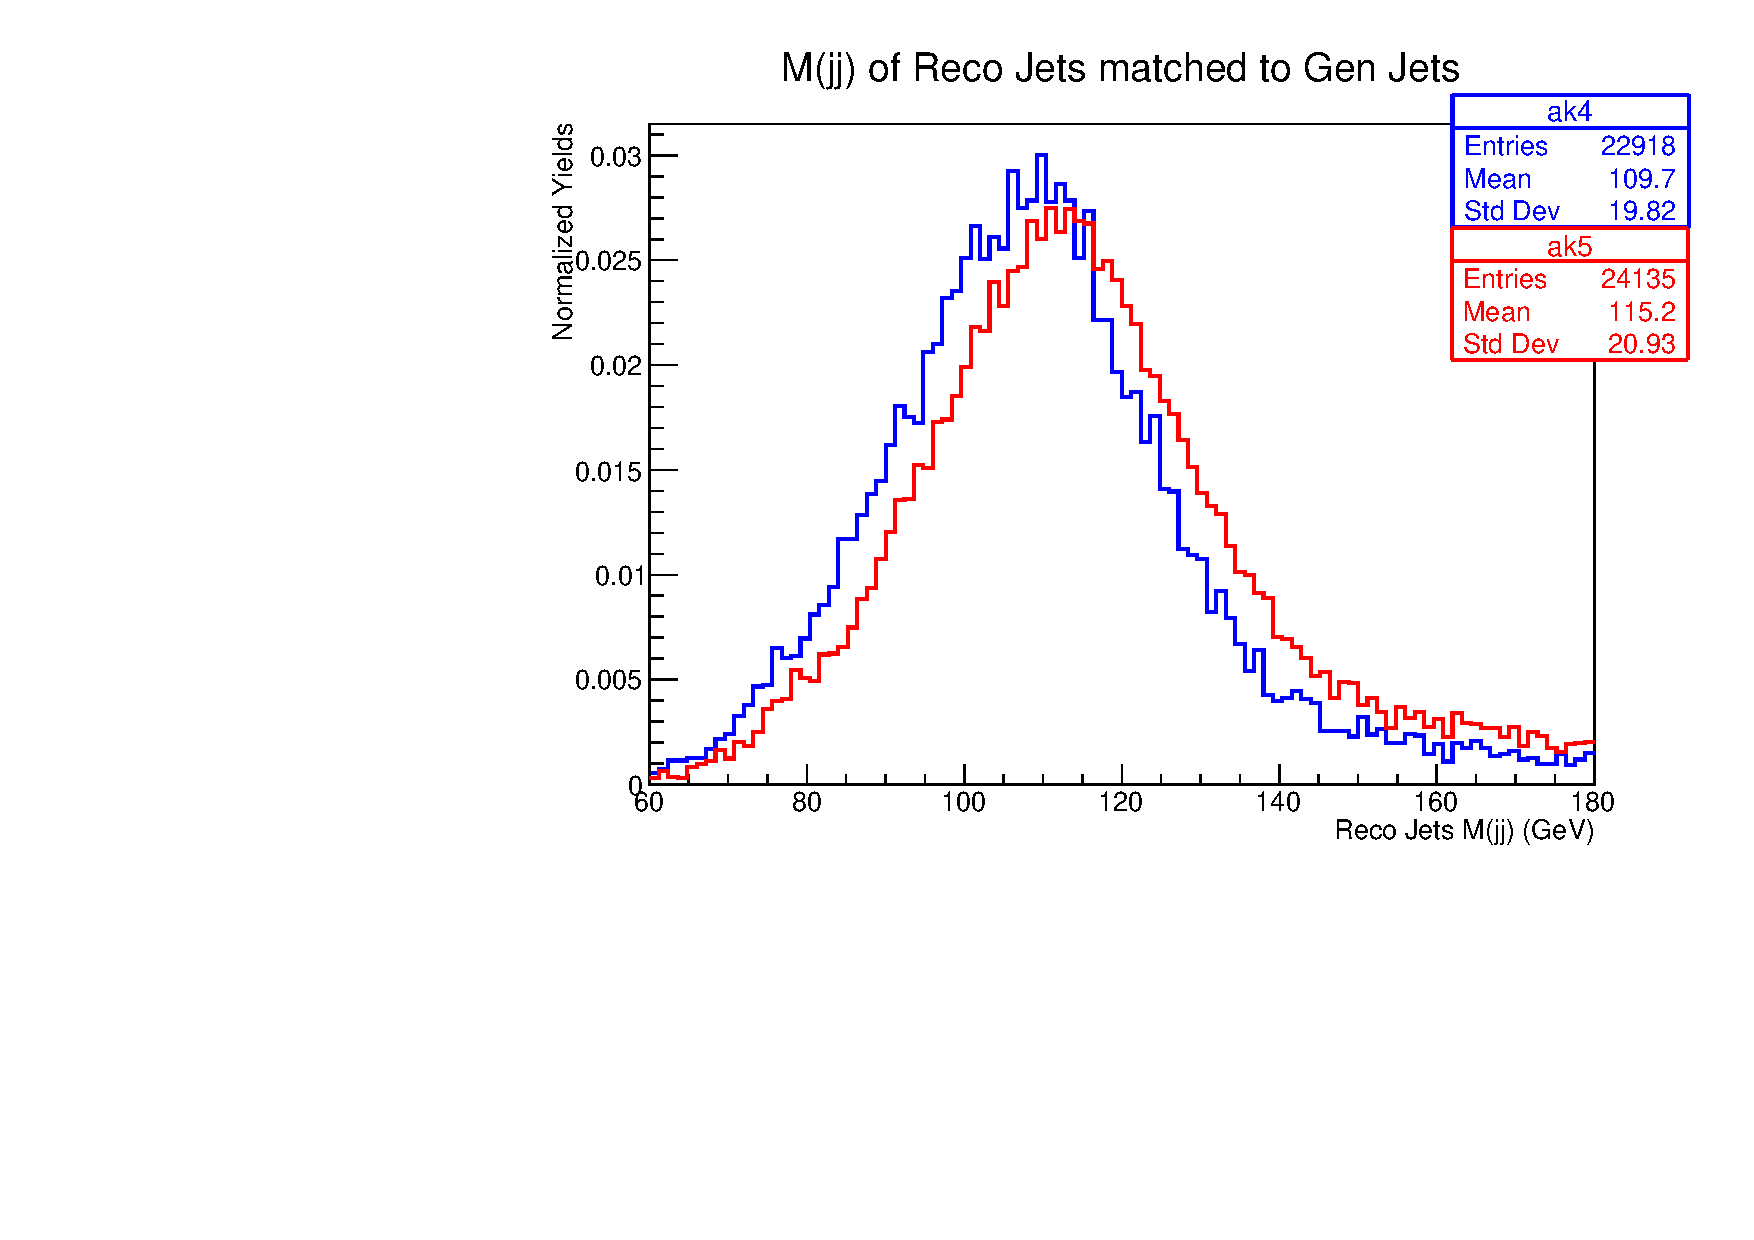
\includegraphics[width=0.45\textwidth]{figures/sec-jets/jet_rec.pdf}\hfil
  \caption{Difference between jet reconstruction used in Run I (red) and Run II (blue)}
  \label{fig:jet-reco}
\end{figure*}

We use the \textit{Loose ID} criteria to select the jets, which is described in
Ref~\cite{jetID-twiki}.

The jet candidates in the event, after passing the aforementioned ID,
must have $\PT > 25 \gev$ and $|\eta| < 2.4$ (so that they are within
the tracker of CMS and can be tagged as coming from $b$ quark). The
jets must also be outside the photon cone with a $\Delta R(j,\gamma) >
0.4$. Dijet objects are then created and only dijets with $\Mjj$ between 60 and 180 GeV 
pass the selection. If more than one dijet has passed those criteria, the dijet with two jets
with highest b-tagging score (see sec. \ref{sec:btag}) are selected as
the dijet candidate.


\subsection{Jet energy regression}
\label{sec:b-reg}

In addition to the misfortune of a small distance parameter of the jet reconstruction algorithm, the energy of the jets coming from $b$-quarks can not be fully reconstructed due to neutrinos escaping the detector. 
In order to improve the \Mjj resolution and gain in S/B discrimination, we employ an energy regression technique on our signal jets. 
The regression technique will work by changing the jet 4-momentum based on the likelihood that this specific jet is a signal jet. 

We use the TMVA package to implement the regression, and it on $X\to\HH\to\bbbb$ MC samples, in order to ensure a statistically independent training. 
Input variables to the training include jet kinematics, energy deposited in the calorimeter, vertex information, and variables related to missing transverse energy of the event (MET) and the distance between the two jets, $\Delta R(j,j)$. 
A summary of all input variables is shown in Table~\ref{tab:reg-vars}.

\begin{table}[h]\centering
\begin{tabular}{rl}
\hline
Input variables        & Jet kinematics: $\eta$, $\PT$, $m_T$\\
as in $\Hbb$ analysis  & Neutral hadron energy fraction, Photon energy fraction\\
regression:       & SecVtxdL, SecVtxdeL, SecVtxPt, SecVtxM, SecVtxNtrk\\
                  & Soft Lepton: \PT, \PT(rel), \DR \\
                  & \PT(Lead Track), Number of verteces\\\hline
\hline
Additional         & \\
variables for our  &\MET, $\Delta\phi(Jet, \MET)$, $\Delta R$(Leading jet, Trailing jet) \\
analysis:          & \\
\hline
\end{tabular}
\caption{Input variables used in TMVA regression. Upper part lists the
  variables that are also used in $\Hbb$ analysis, and the lower part
  lists additional variables.}
\label{tab:reg-vars}
\end{table}

The target for the regression training is $\PT^{gen}/\PT^{reco}$, where the generated level jet ("gen") contains neutrinos. 
This means that the regression technique will aim to construct, in a piece-wise manner, a function $f(\bar{x}) = \langle \PT^{gen}/\PT^{reco} \rangle (\bar{x})$, where $\bar{x}$ are the regression input variables, which can be used to correct the jet's energy. 
The standard gen-jet collection in CMS does not include the neutrinos, so we add them manually from gen-particle collection, using $\DR$ cone of 0.4 for matching.

Adding neutrinos to the gen-jet brings the energy of the jet closer to the energy of original b-quark, which is illustrated in Fig.~\ref{fig:b-reg-quark}.  
Figure~\ref{fig:b-reg-quark} also shows additional distributions, also comparing the gen-jets with and without
neutrino additions: \PT of the leading and trailing jets, invariant mass of the Higgs boson candidates and the $m_{jjjj}$. 
Events from all mass samples are combined, which explains the shape of $m_{jjjj}$ distribution. 
From these figures one can see the effects on the mass resolution of adding neutrinos to gen-jets.

\begin{figure*}[h]
  \centering
  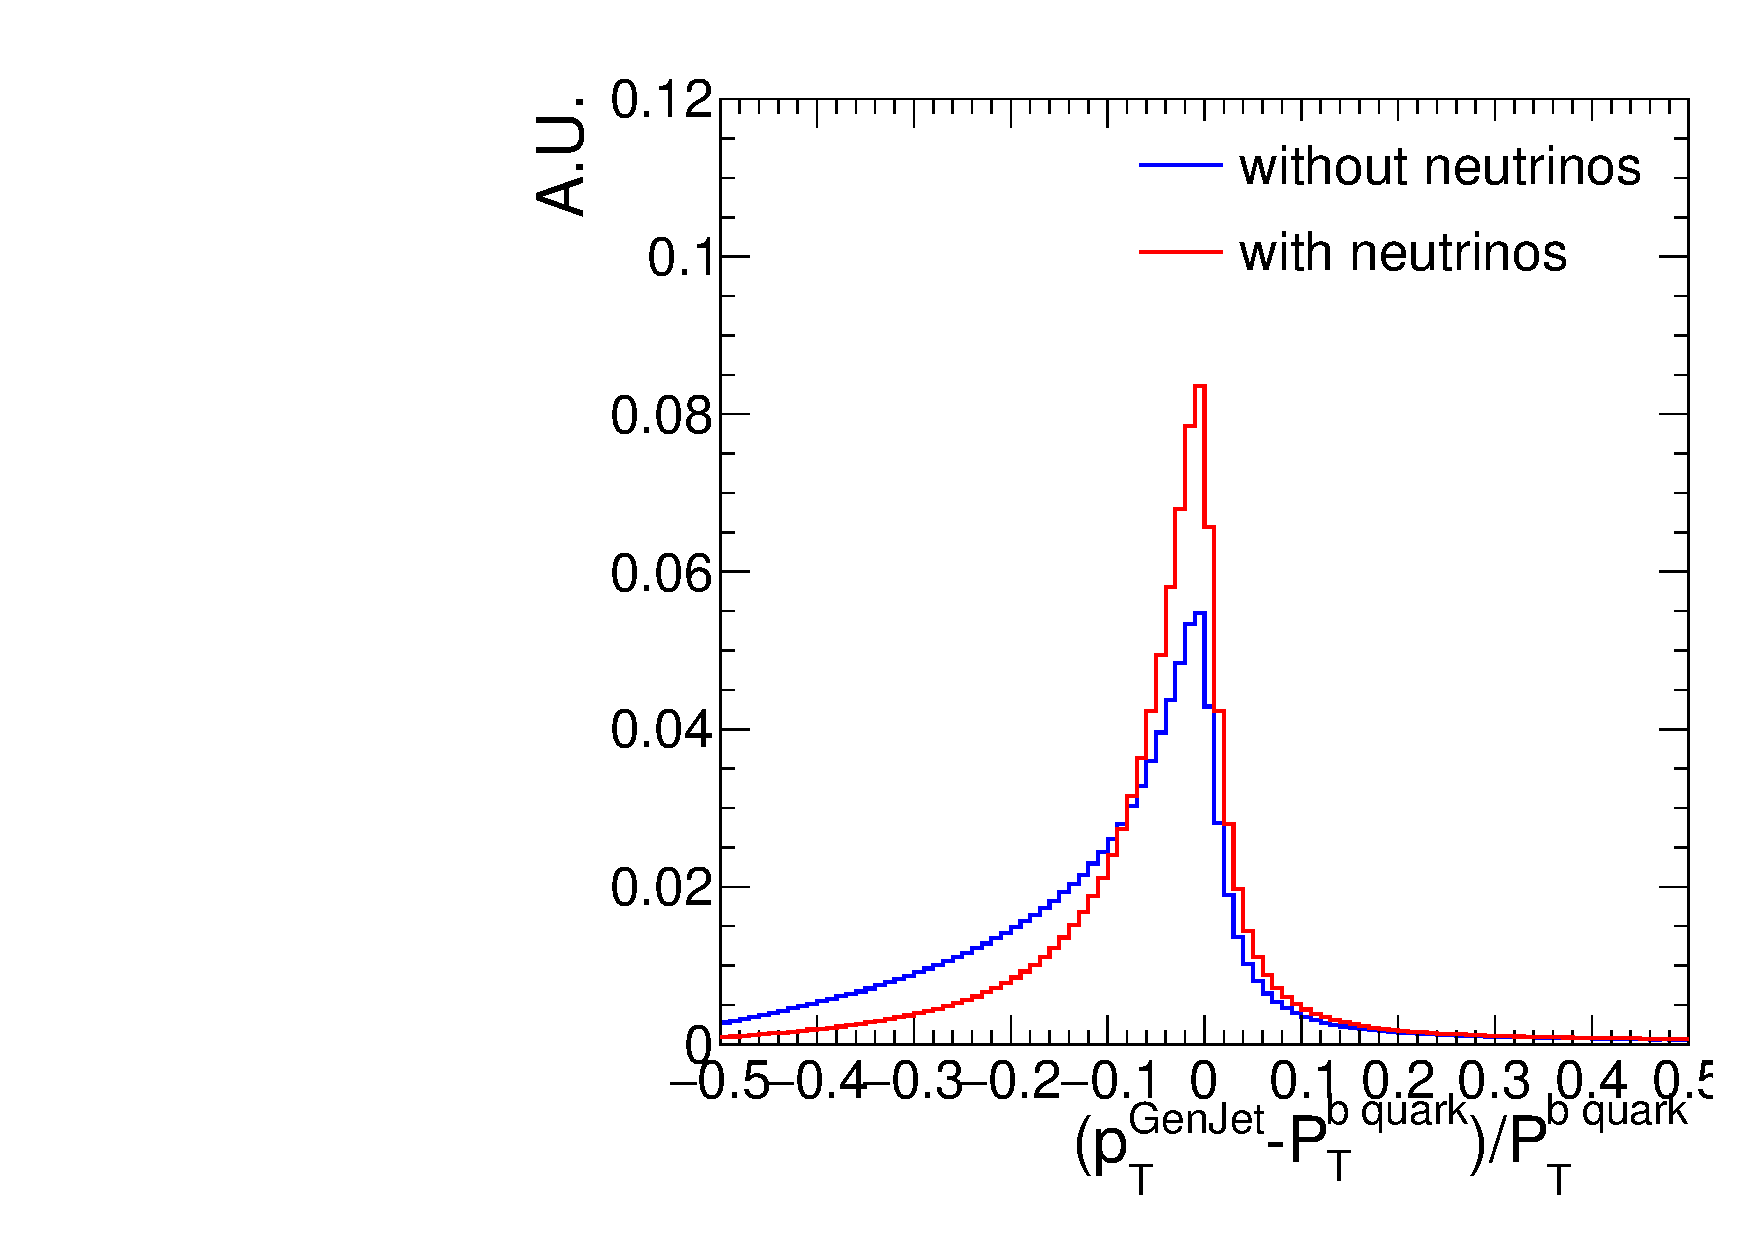
\includegraphics[width=0.33\textwidth]{b-reg/input_noBins_GenJetPtGenPtRel}\hfil
  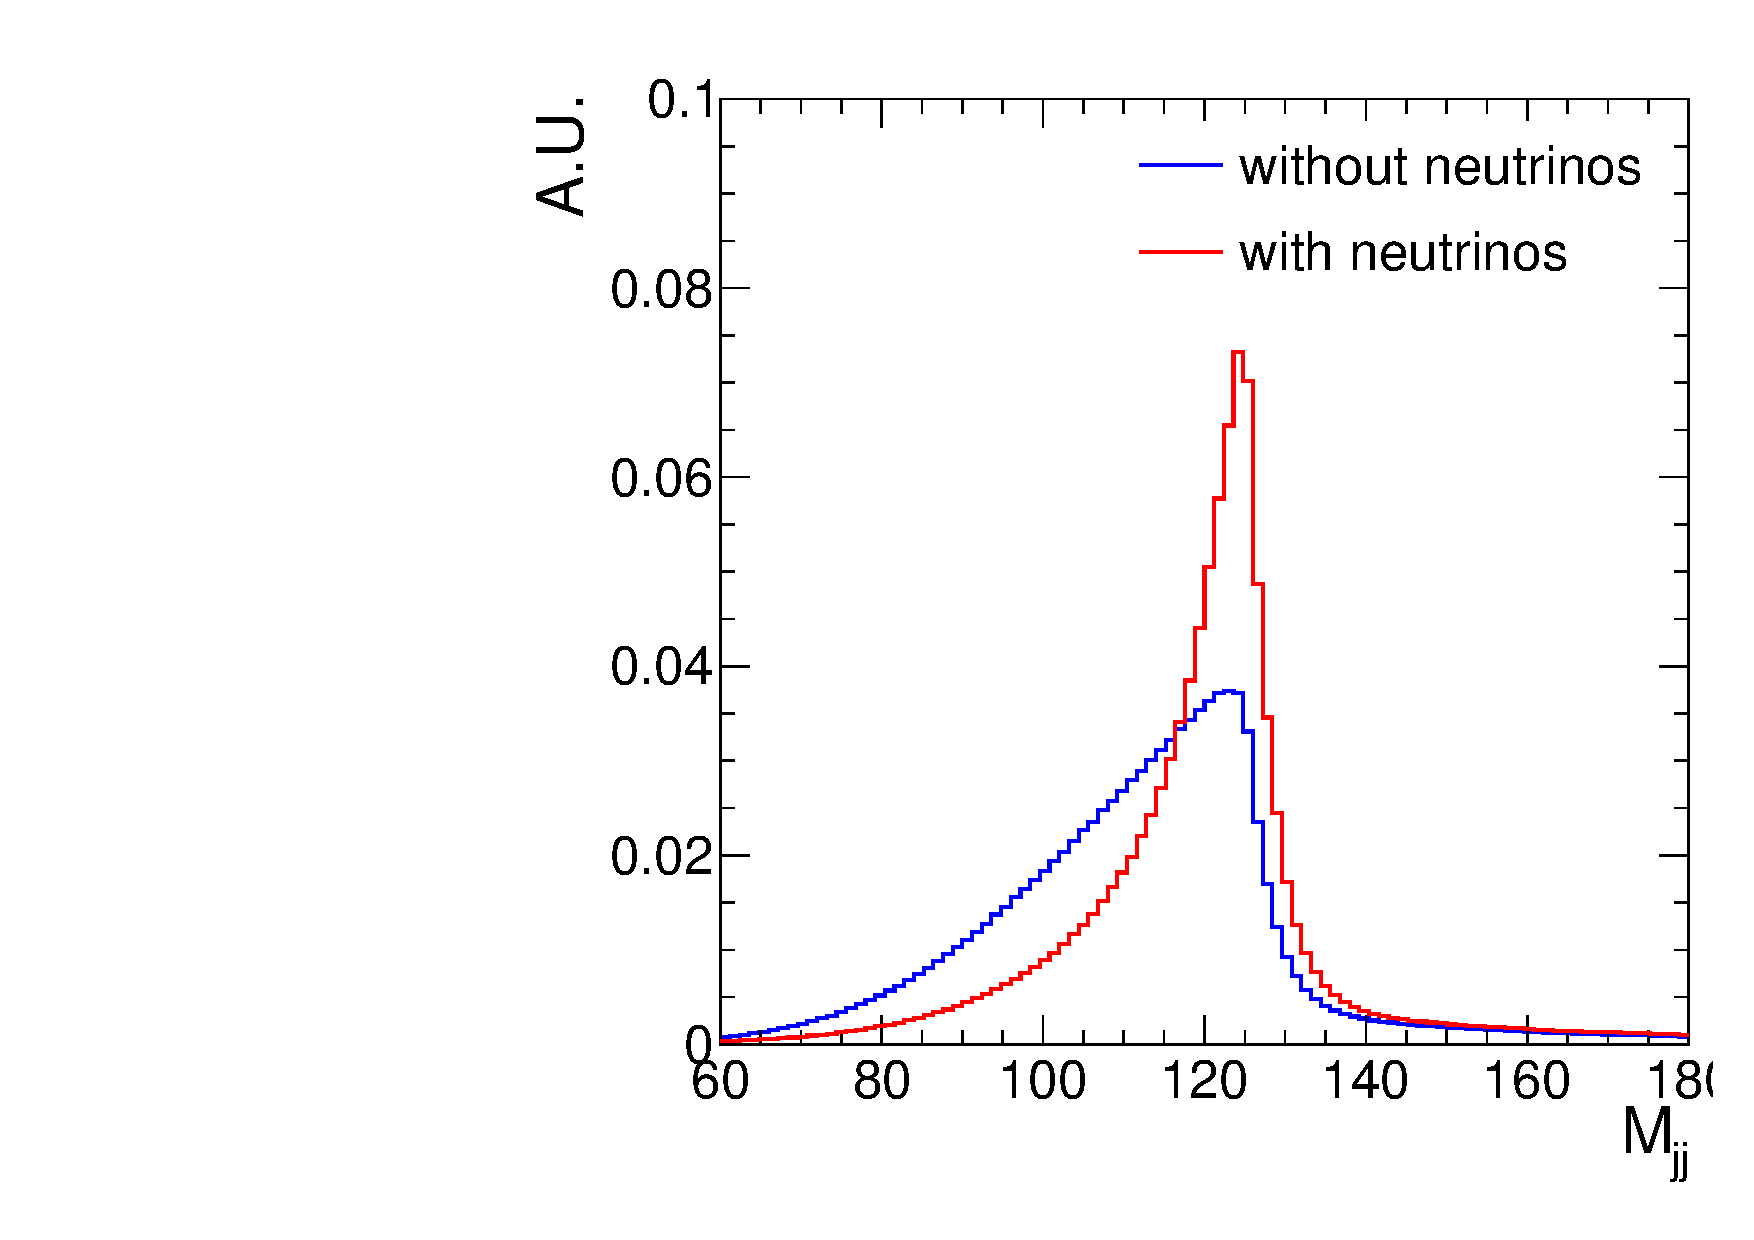
\includegraphics[width=0.33\textwidth]{b-reg/input_noBins_jjMass_Jetgenjet}\hfil
  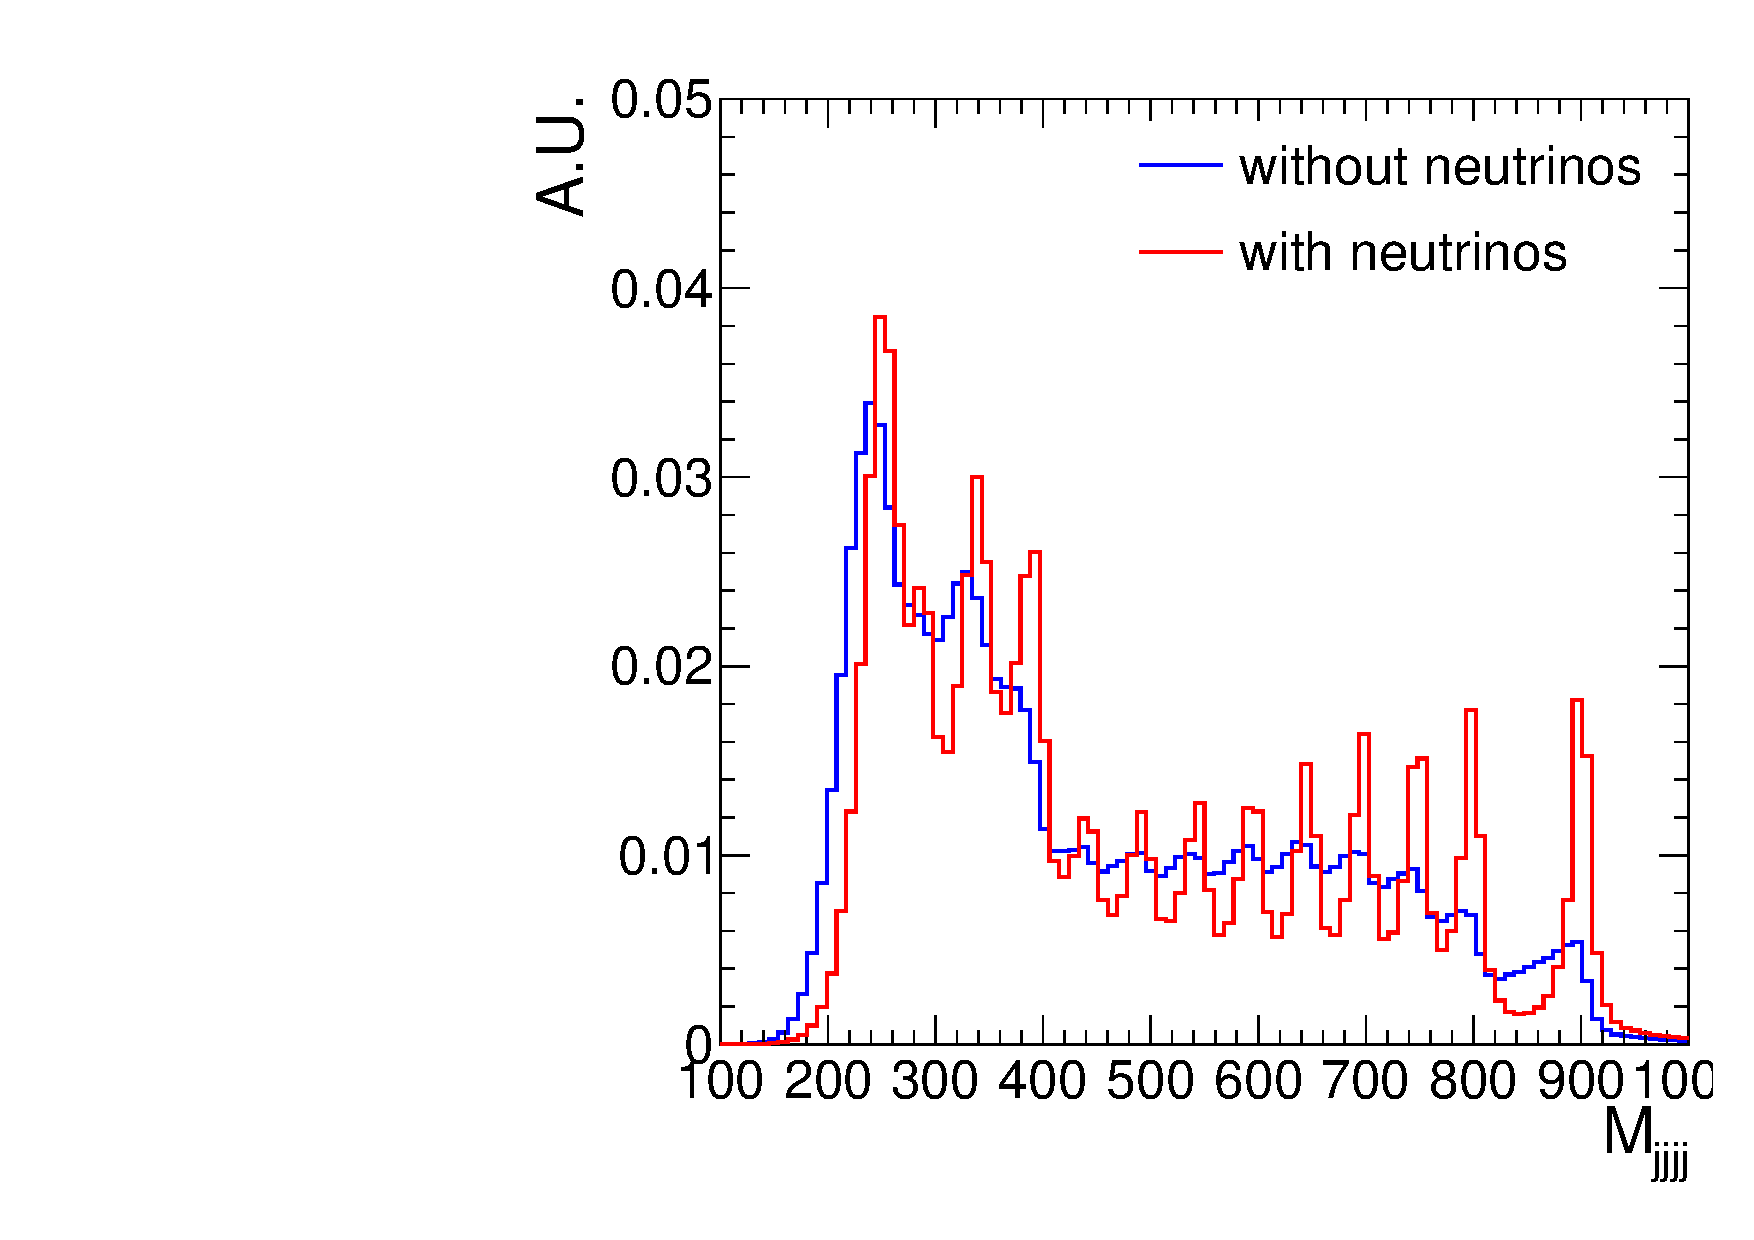
\includegraphics[width=0.33\textwidth]{b-reg/input_noBins_jjjjMass_Jetgenjet}\hfil

  \caption{Relative \PT difference, $m_{jj}$ and $m_{jjjj}$ distributions of the b-quark and the
    corresponding gen-jet, obtained from $\HH\to\bbbb$ samples. Red
    histogram is for gen-jets containing neutrinos, blue is for jets
    without neutrinos.}
  \label{fig:b-reg-quark}
\end{figure*}

For the training we select jets that satisfy the following criteria:
\begin{itemize}
\item $\PT > 20\GeV$, $|\eta| < 2.4$
\item Matched to the generated level jet within a cone $\DR<0.4$ (this matching is done as part of MiniAOD reconstruction)
\item Matched to a b-quark within a cone $\DR<0.4$
\end{itemize}


We perform six different trainings to check the impact of additional variables:
\begin{itemize}
\item Using 15 variables based on $\Hbb$ training, listed in
  Table~\ref{tab:reg-vars}. It is denoted as \textbf{Baseline} on the
  figures below.
\item Using 15 variables plus \MET and $\Delta\phi(Jet, \MET)$.
\item Using 15 variables plus \MET , $\Delta\phi(Jet, \MET)$, and also
  $\Delta R$(Leading jet, Trailing jet).  This training is denoted as
  \textbf{full 15+3var} in the text.
\item Using 15 variables as above but in addition, for each pair of
  jets from the Higgs boson, the training is performed separately for
  the leading and trailing jets. That is, two XML weight files are
  derived, one for the leading and one for the trailing jet in the
  event.  This method is denoted as \textbf{js} on the figures and in
  the text.
\item Using 15 plus \MET and $\Delta\phi(Jet, \MET)$ variables, and
  separating the training for leading and trailing jets as above.
\item Using 15 plus \MET, $\Delta\phi(Jet, \MET)$ and $\Delta R$
  variables, and separating the training for leading and trailing jets
  as above.
\end{itemize}

The regression is performed with the TMVA package, using the Boosted Decision Tree technique with gradient boosting. 500 decision trees with depth 5 are created to estimate the target. 
The pruning technique is applied.
The detailed TMVA modified options are as follows:

\verb|NTrees=500:MaxDepth=5:nCuts=500:BoostType=Grad:!UseBaggedGrad|

\verb|Shrinkage=0.1:MinNodeSize=1:PruneStrength=5:PruneMethod=CostComplexity|

\verb|NegWeightTreatment=IgnoreNegWeightsInTraining|

After the training is done, its performance is checked in signal samples, $X\to\HH\to\ggbb$, at all mass points of $m_X$.  
The selection is the same as the training samples. 
All of our trainings are compared with the one done by $\Hbb$ analysis, which is denoted as \textbf{Hbb} on the figures. 
The $\PT^{reco}$ of the reconstructed jet can be compared to the target $\PT^{gen}$ of the generated jet with neutrinos. 
An example of such distributions is shown in Fig.~\ref{fig:b-reg-pt-res} for the leading and trailing jets. 
From distributions such as in Fig.~\ref{fig:b-reg-pt-res} we obtain the mean value for the \textbf{scale} and sigma ($\sigma$) for the \textbf{resolution}. 
The mean value and sigma are obtained from the Bukin function fit. 
The scale and resolution of the leading and trailing jets versus their \PT are shown in Fig.~\ref{fig:b-reg-jet-res}. 
From this figure we can conclude that adding MET variables into the training improves significantly the resolution. 
As expected the \textbf{15+3var js} training gives best per-jet resolution across the whole \PT range.

\begin{figure*}[h]
  \centering
  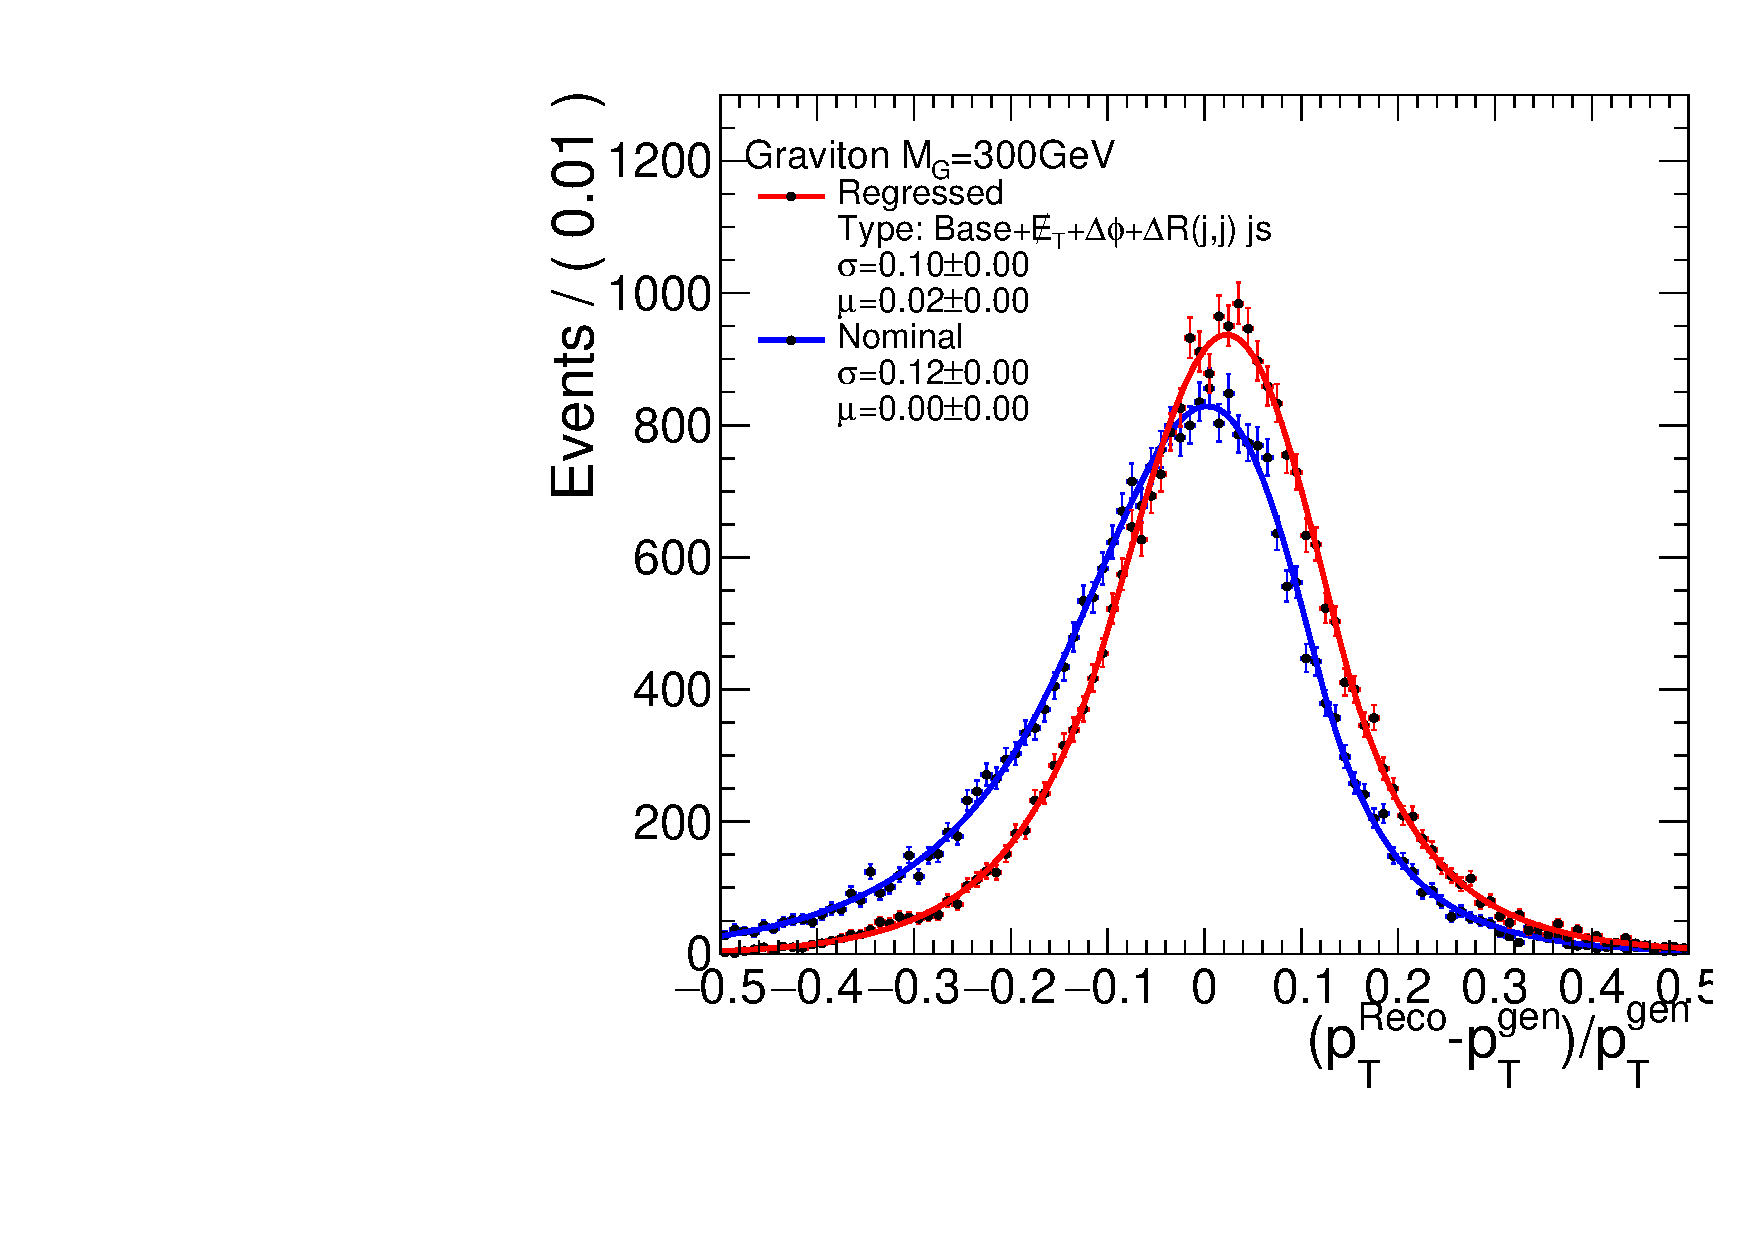
\includegraphics[width=0.35\textwidth]{b-reg/AN_mass300_J1}\hfil
  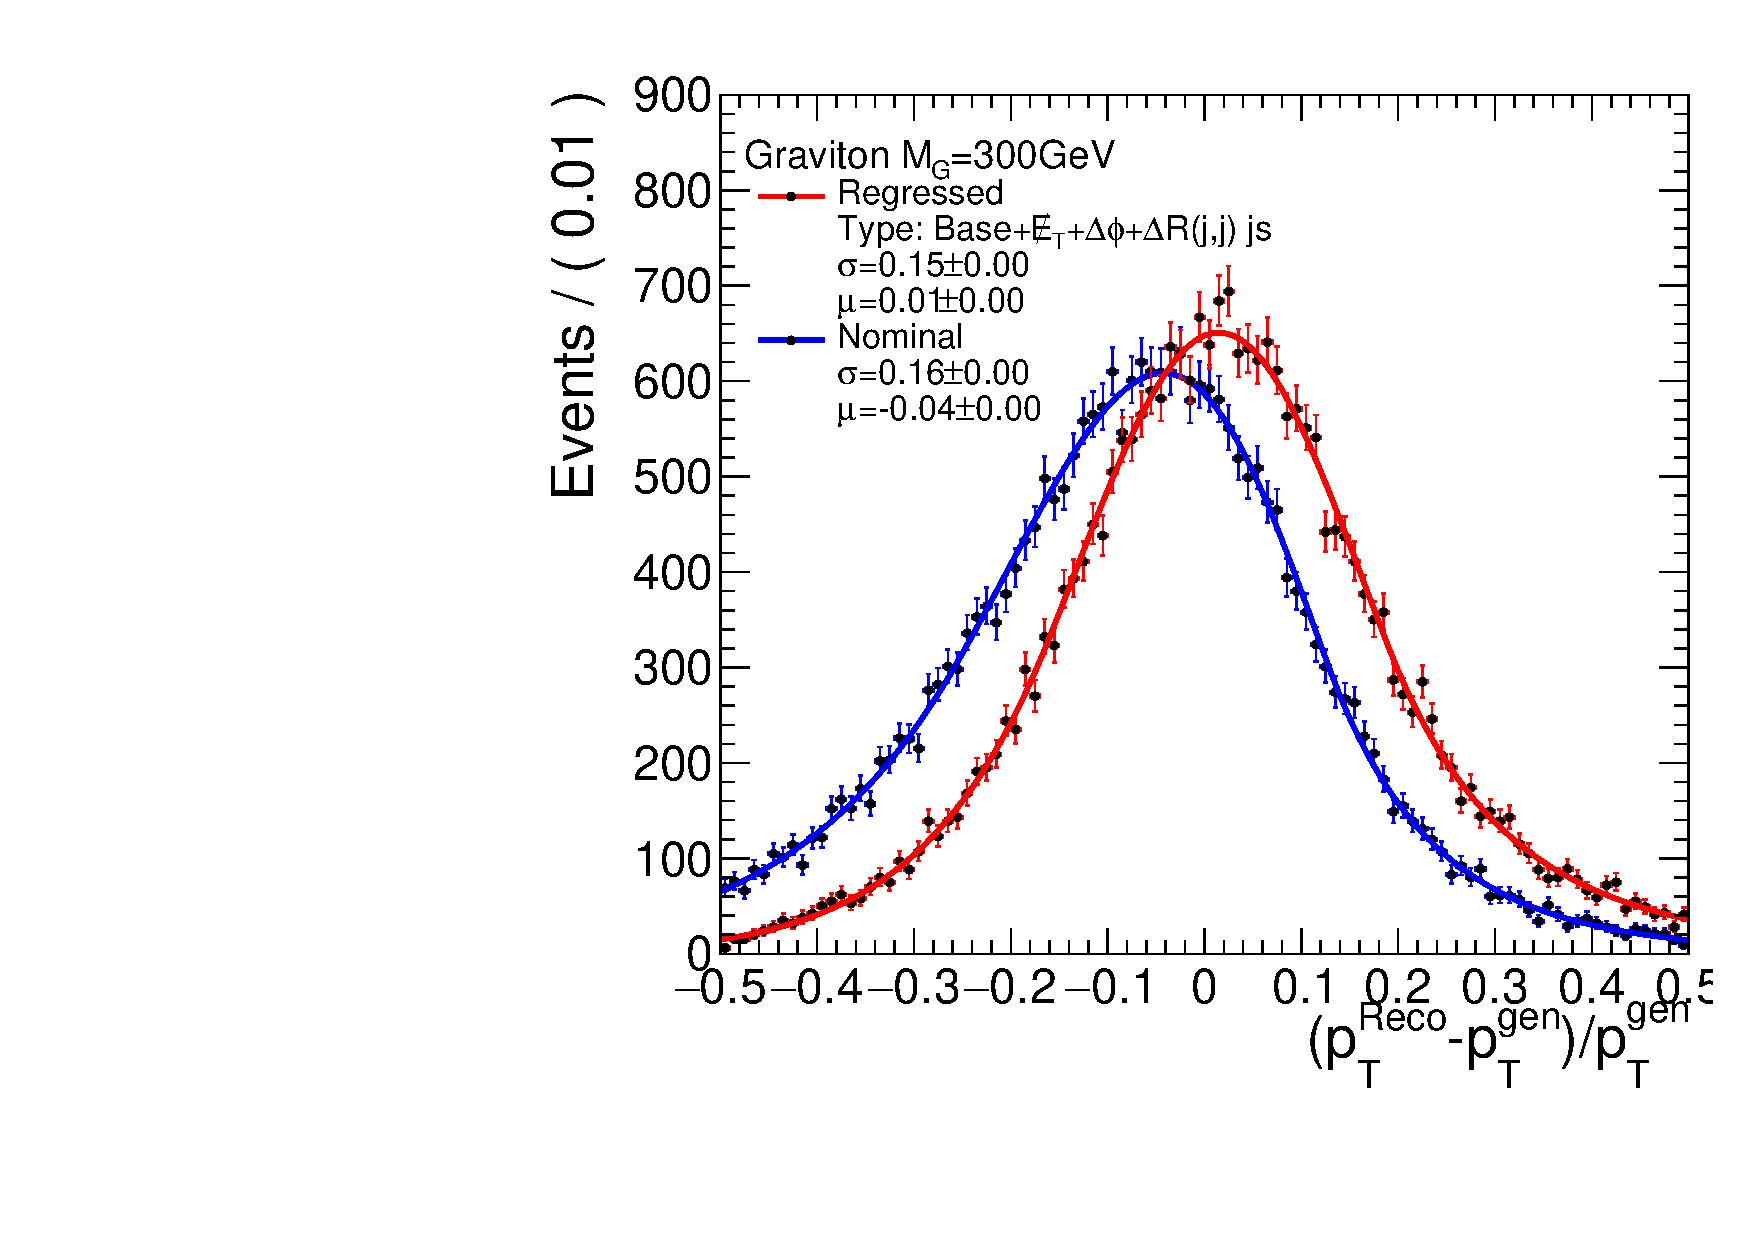
\includegraphics[width=0.35\textwidth]{b-reg/AN_mass300_J2}\hfil
  \caption{Relative \PT difference of the reconstructed and generated
    level jets after regression (red histograms) and without
    the regression (blue histograms).}
  \label{fig:b-reg-pt-res}
\end{figure*}

\begin{figure*}[h]
  \centering
  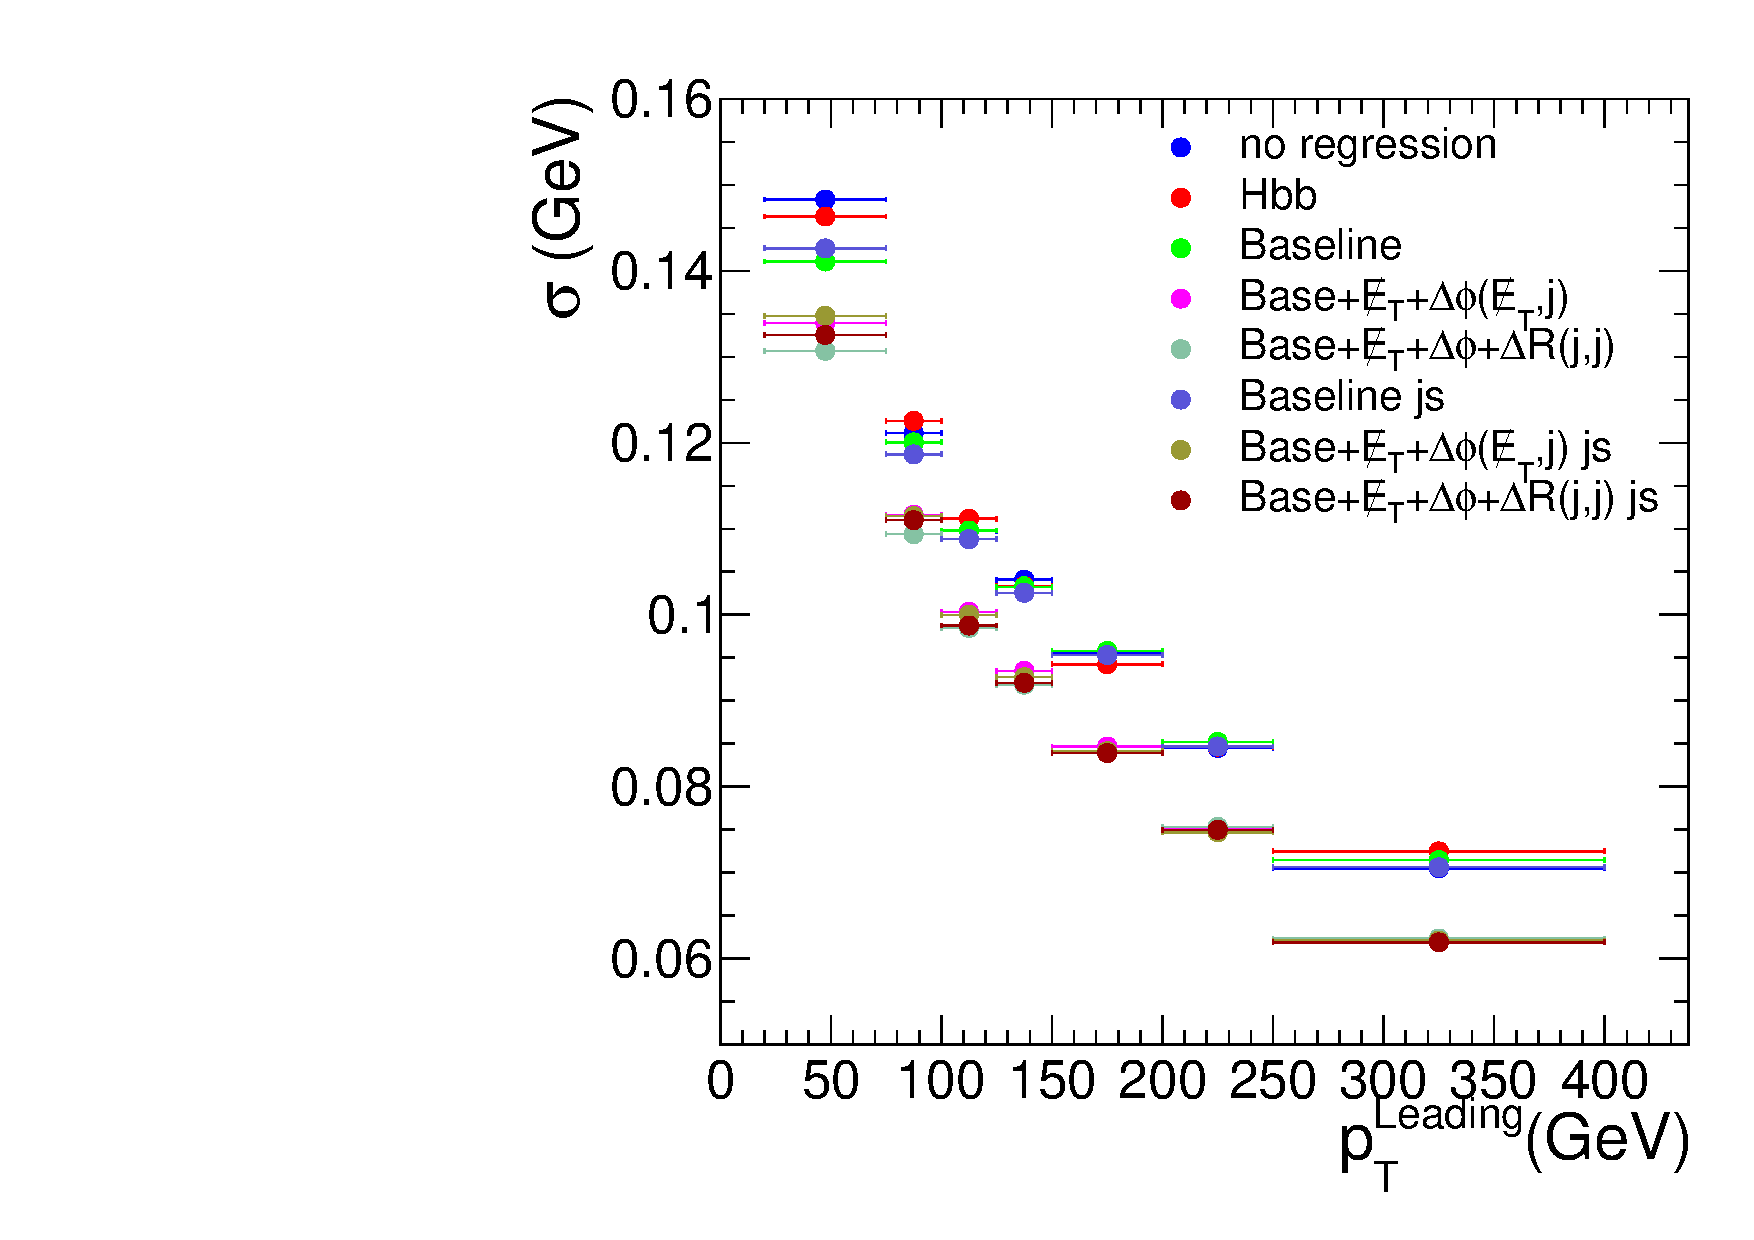
\includegraphics[width=0.35\textwidth]{b-reg/AN_HHbbgg_G_sigma_jet1pT}\hfil
  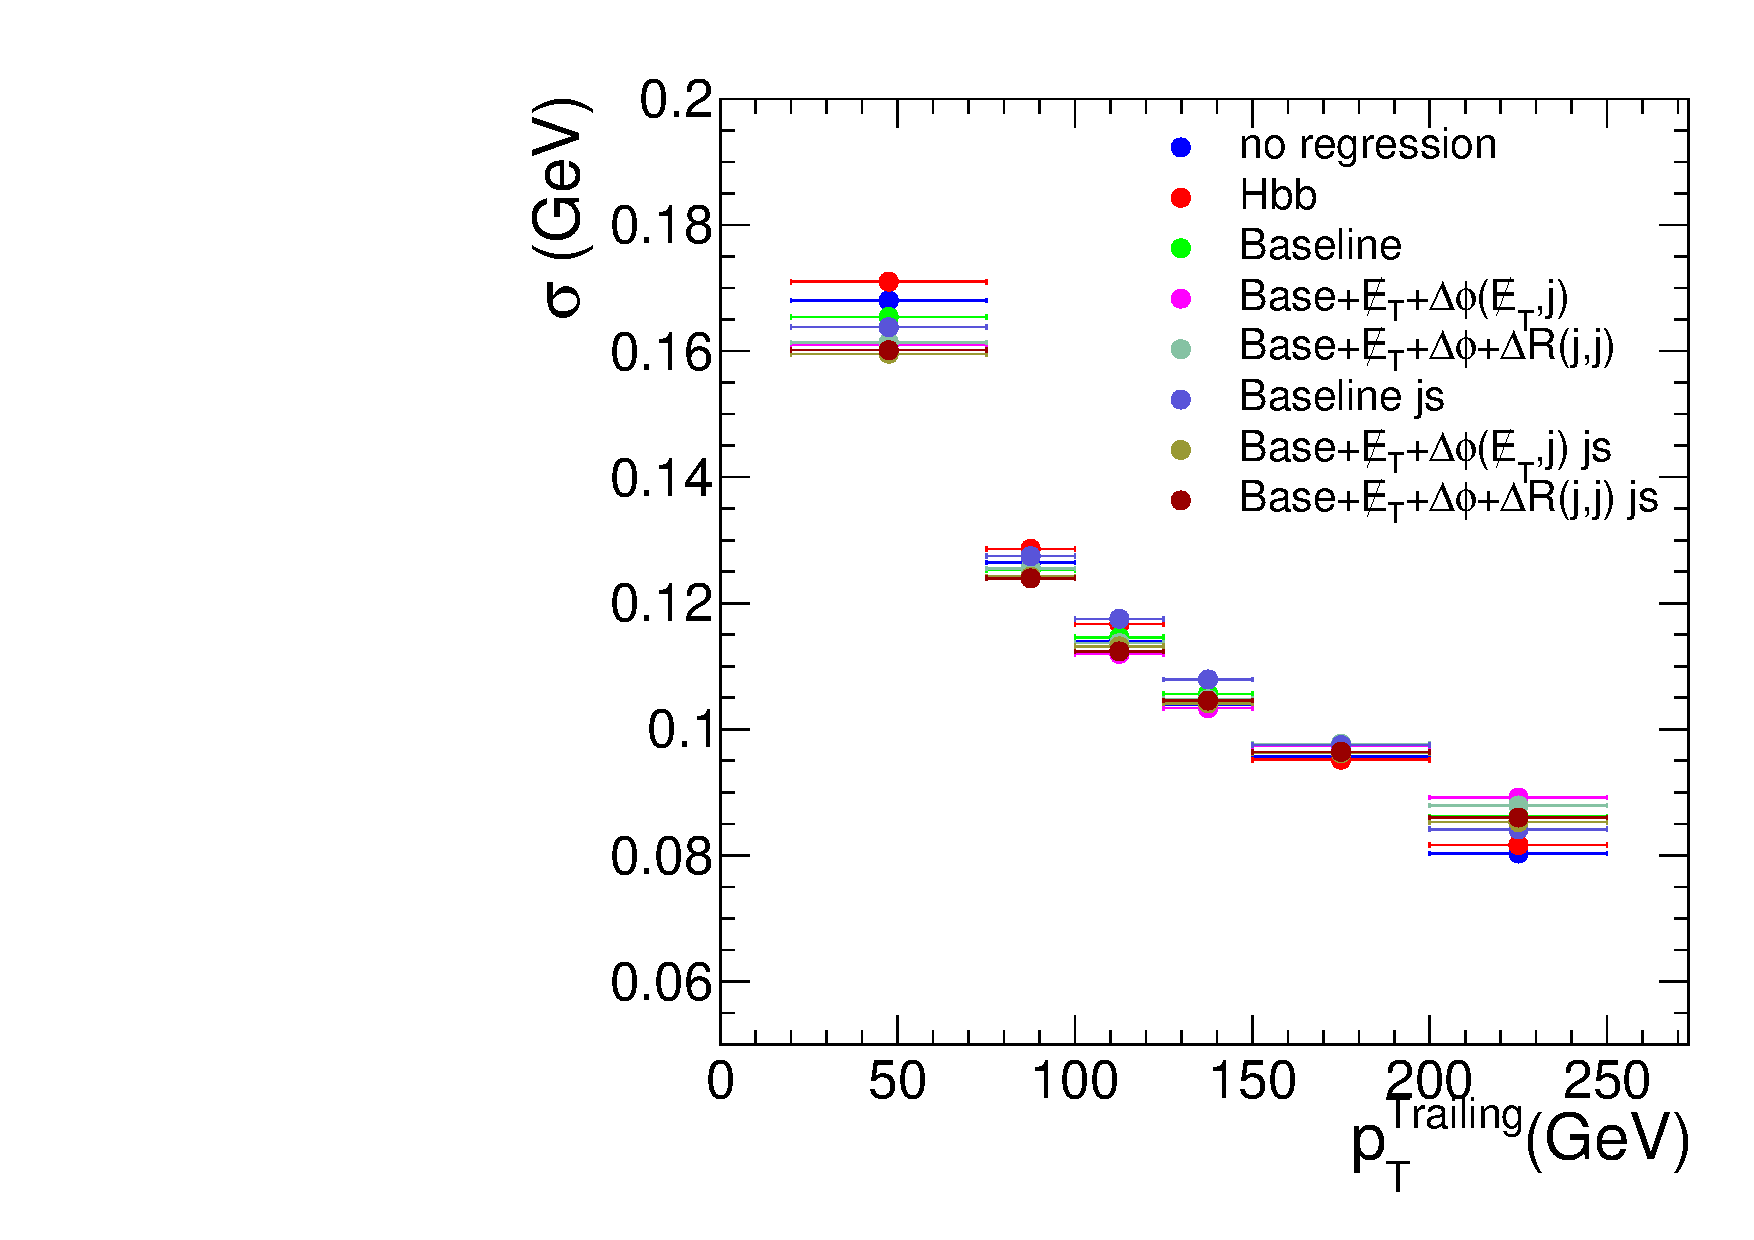
\includegraphics[width=0.35\textwidth]{b-reg/AN_HHbbgg_G_sigma_jet2pT}\hfil\\
  \caption{The resolution of the jet \PT for leading (left) and trailing (right) jets from the signal
    sample $G\to\HH\to\ggbb$.}
  \label{fig:b-reg-jet-res}
\end{figure*}
  
  \begin{figure*}[h]
  \centering
  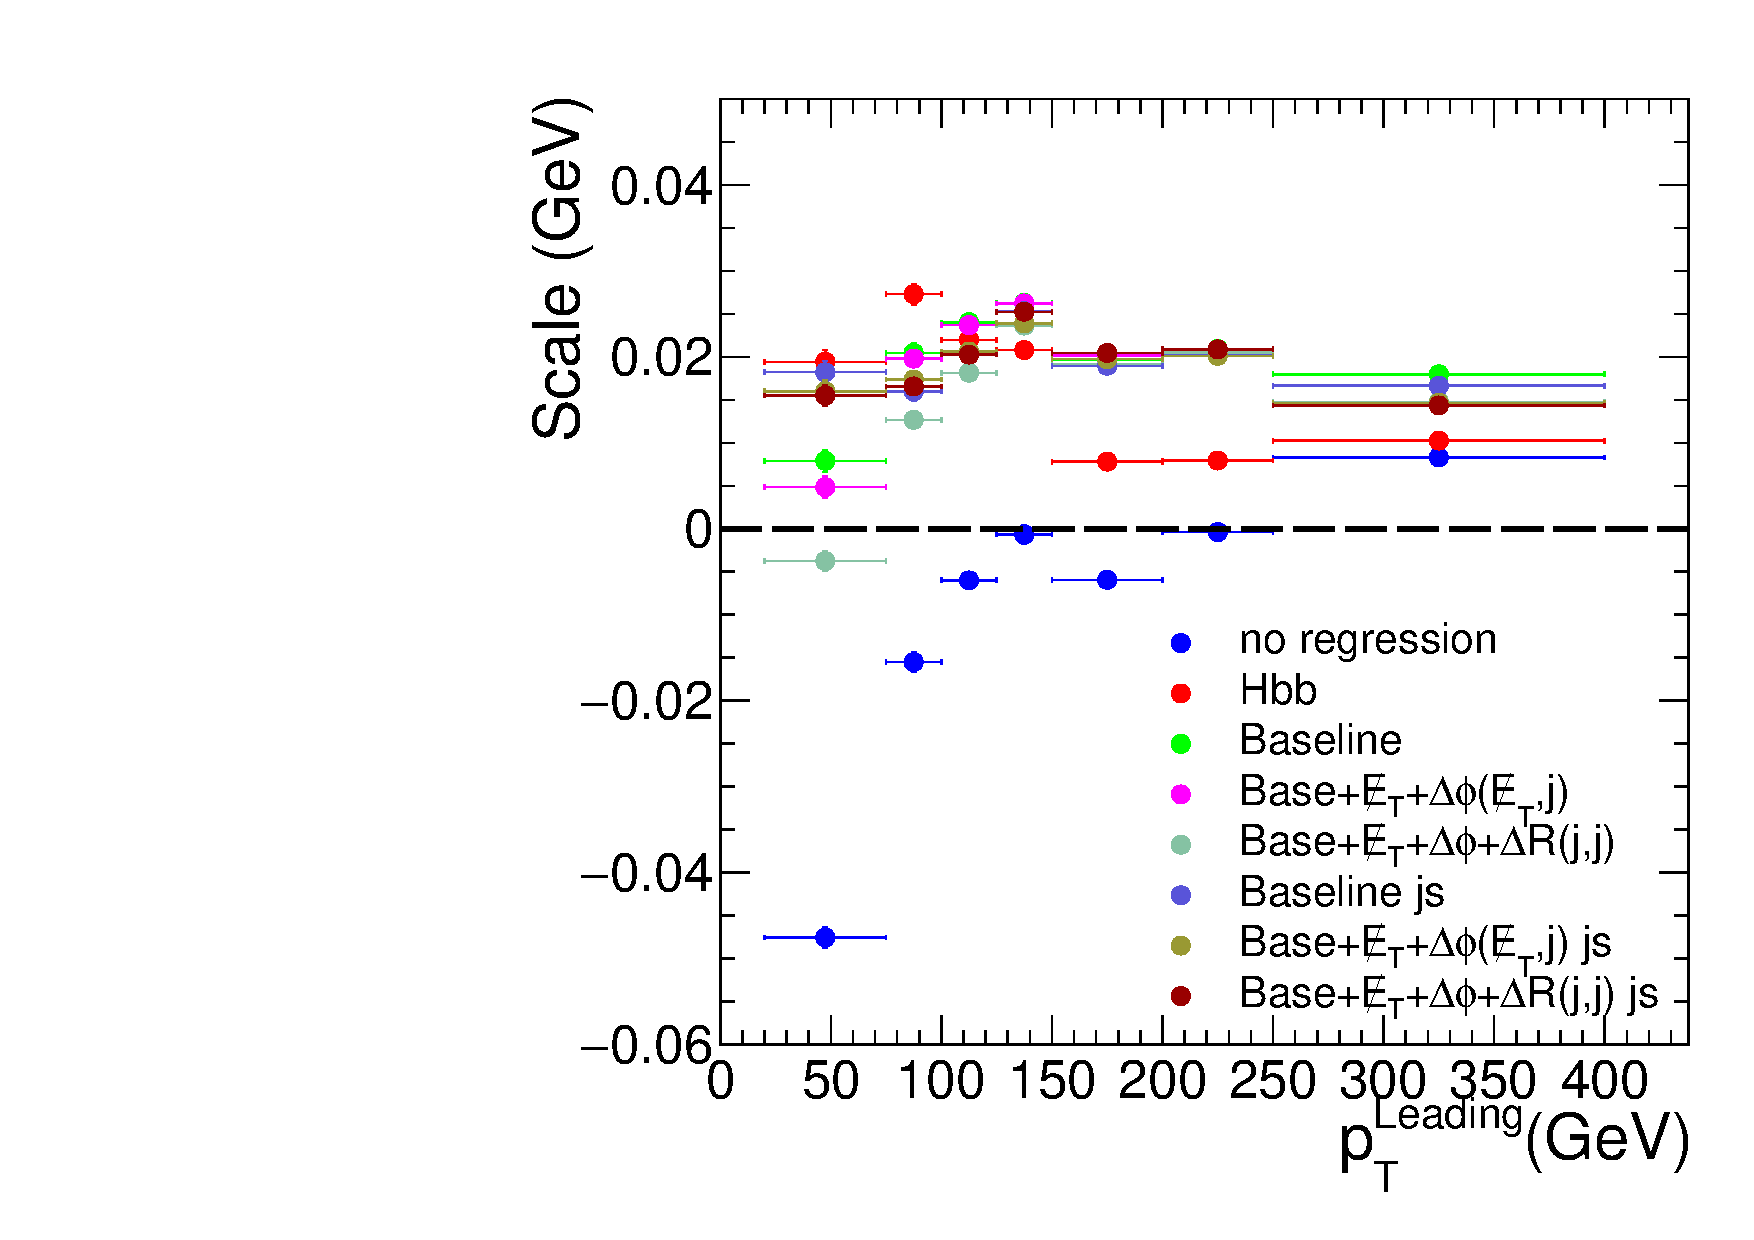
\includegraphics[width=0.35\textwidth]{b-reg/AN_HHbbgg_G_scale_jet1pT}\hfil
  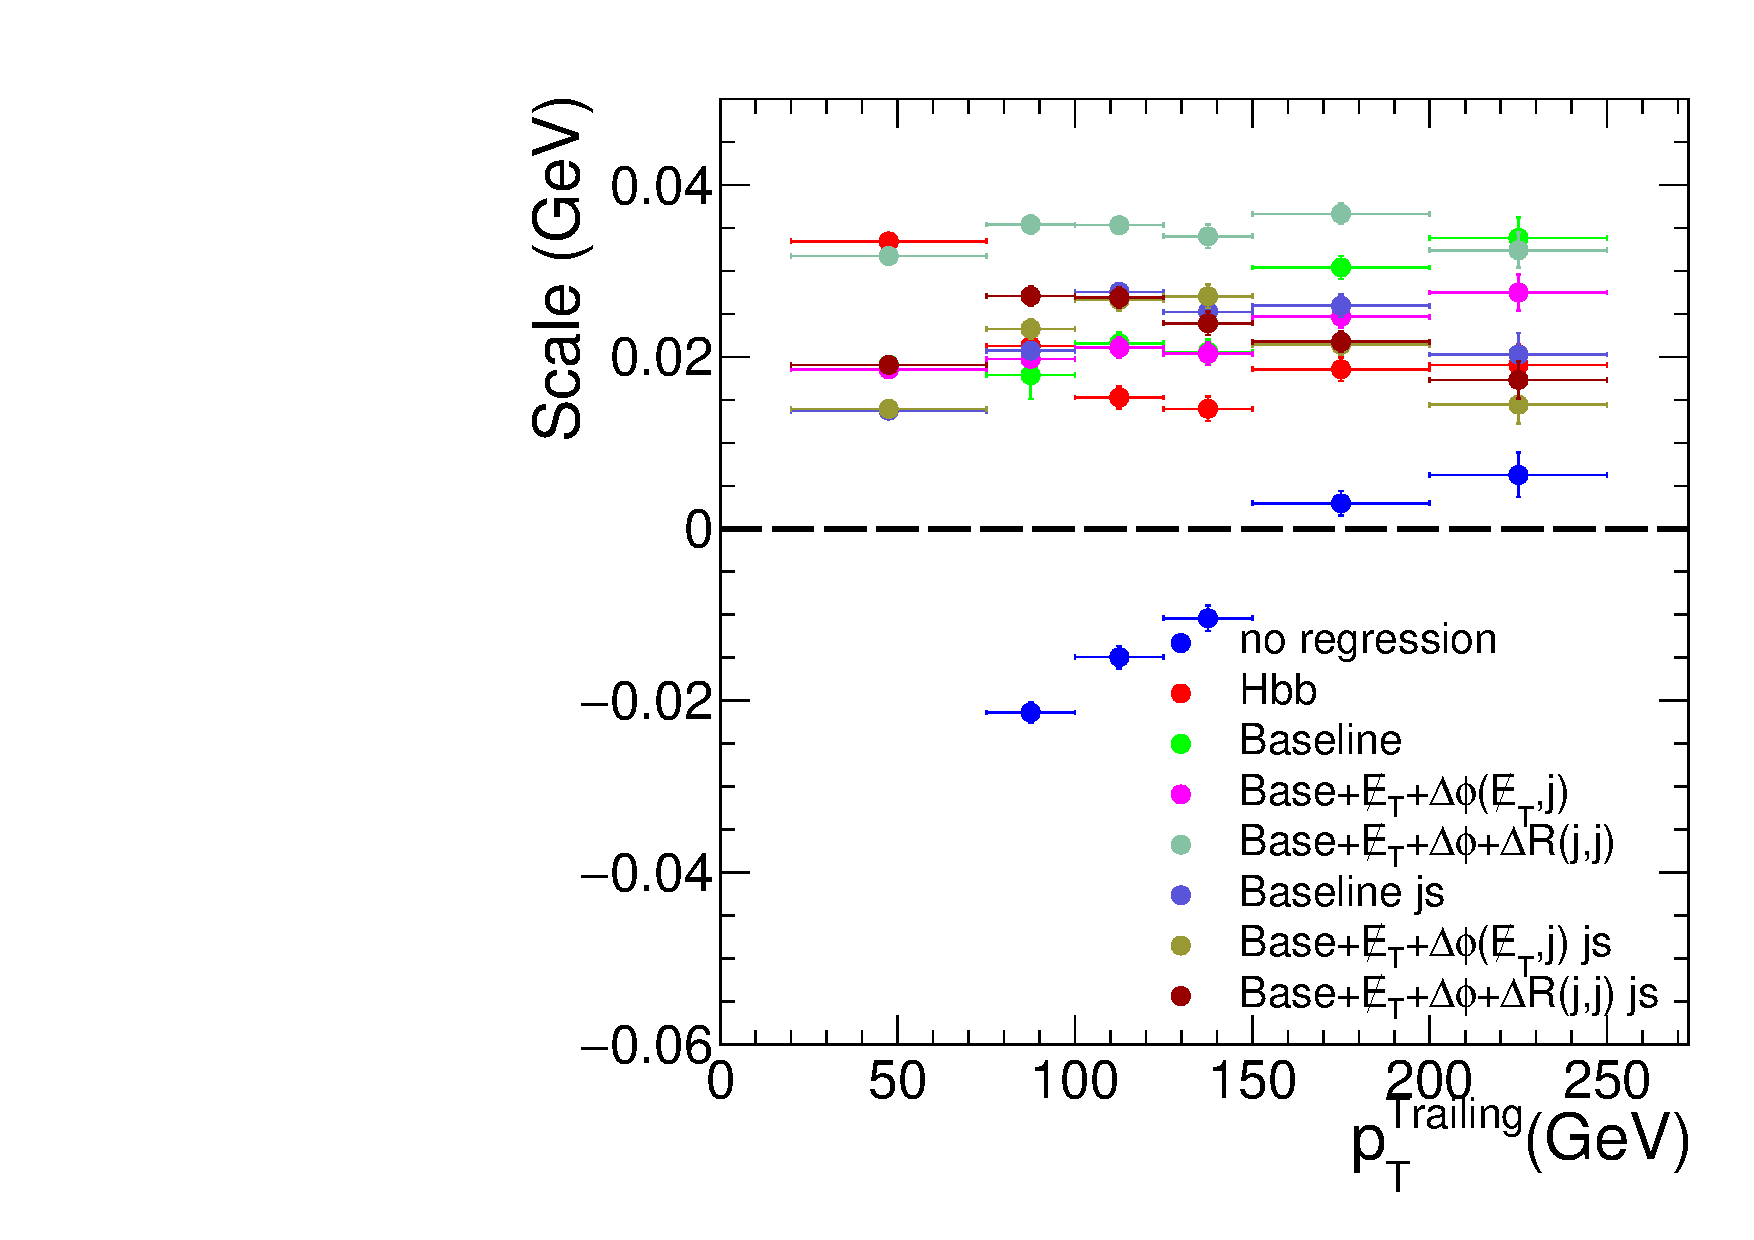
\includegraphics[width=0.35\textwidth]{b-reg/AN_HHbbgg_G_scale_jet2pT}\hfil\\
  \caption{The scale of the jet \PT for leading (left) and trailing (right) jets from the signal
    sample $G\to\HH\to\ggbb$.}
  \label{fig:b-reg-jet-scale}
\end{figure*}

The purpose of the regression is to improve the Higgs boson mass resolution from the $\Hbb$ decay in $X\to\HH\to\ggbb$ signal.  
The distributions together with the fit by Bukin function are shown in Figs.~\ref{fig:b-reg-mH-fit-reco}, where the reconstructed mass is shown after the \textbf{full 15+3var js} regression training, for $m_G = 300\GeV$ and $m_G = 900\GeV$.

After the fitting to the corresponding function is done, we obtain the mean and the width parameters of the fit.  
The width and mean (both in \GeV) are shown on Fig.~\ref{fig:b-reg-mH-res} versus the mass of the Graviton particle.  
From this figure we arrive at the same conclusion  as for single-jet plots of Fig.~\ref{fig:b-reg-jet-res}: the MET variables improve the resolution and the \textbf{full 15+3var js} training gives the best mass resolution. 
The training with \textbf{15} variables give similar results to the \textbf{Hbb} training.  
In all trainings the scale does not match the nominal value of the Higgs boson mass. 
This is expected because the jets (both at reco and gen levels) do not contain the whole energy of the Higgs boson decay.

\begin{figure*}[h]
  \centering
  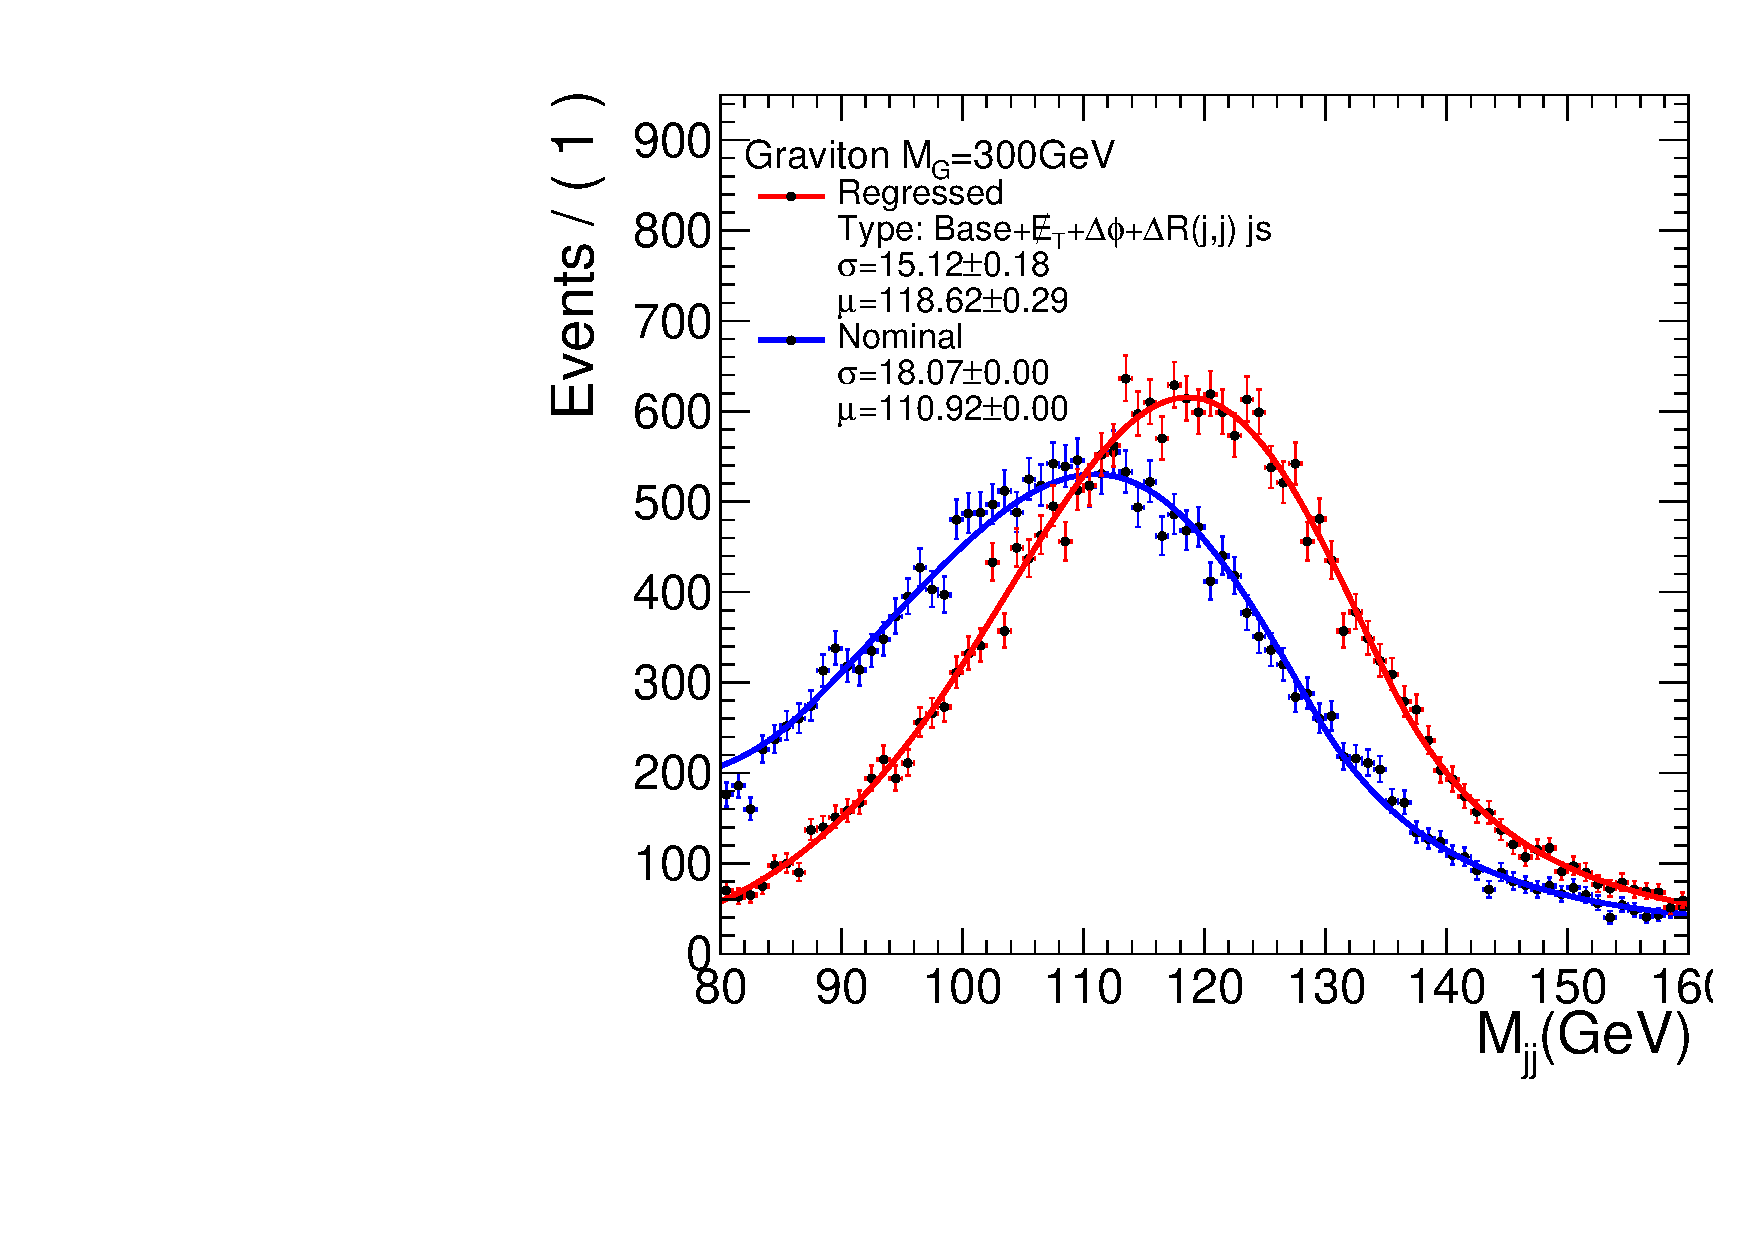
\includegraphics[width=0.35\textwidth]{b-reg/AN_mass300}\hfil
  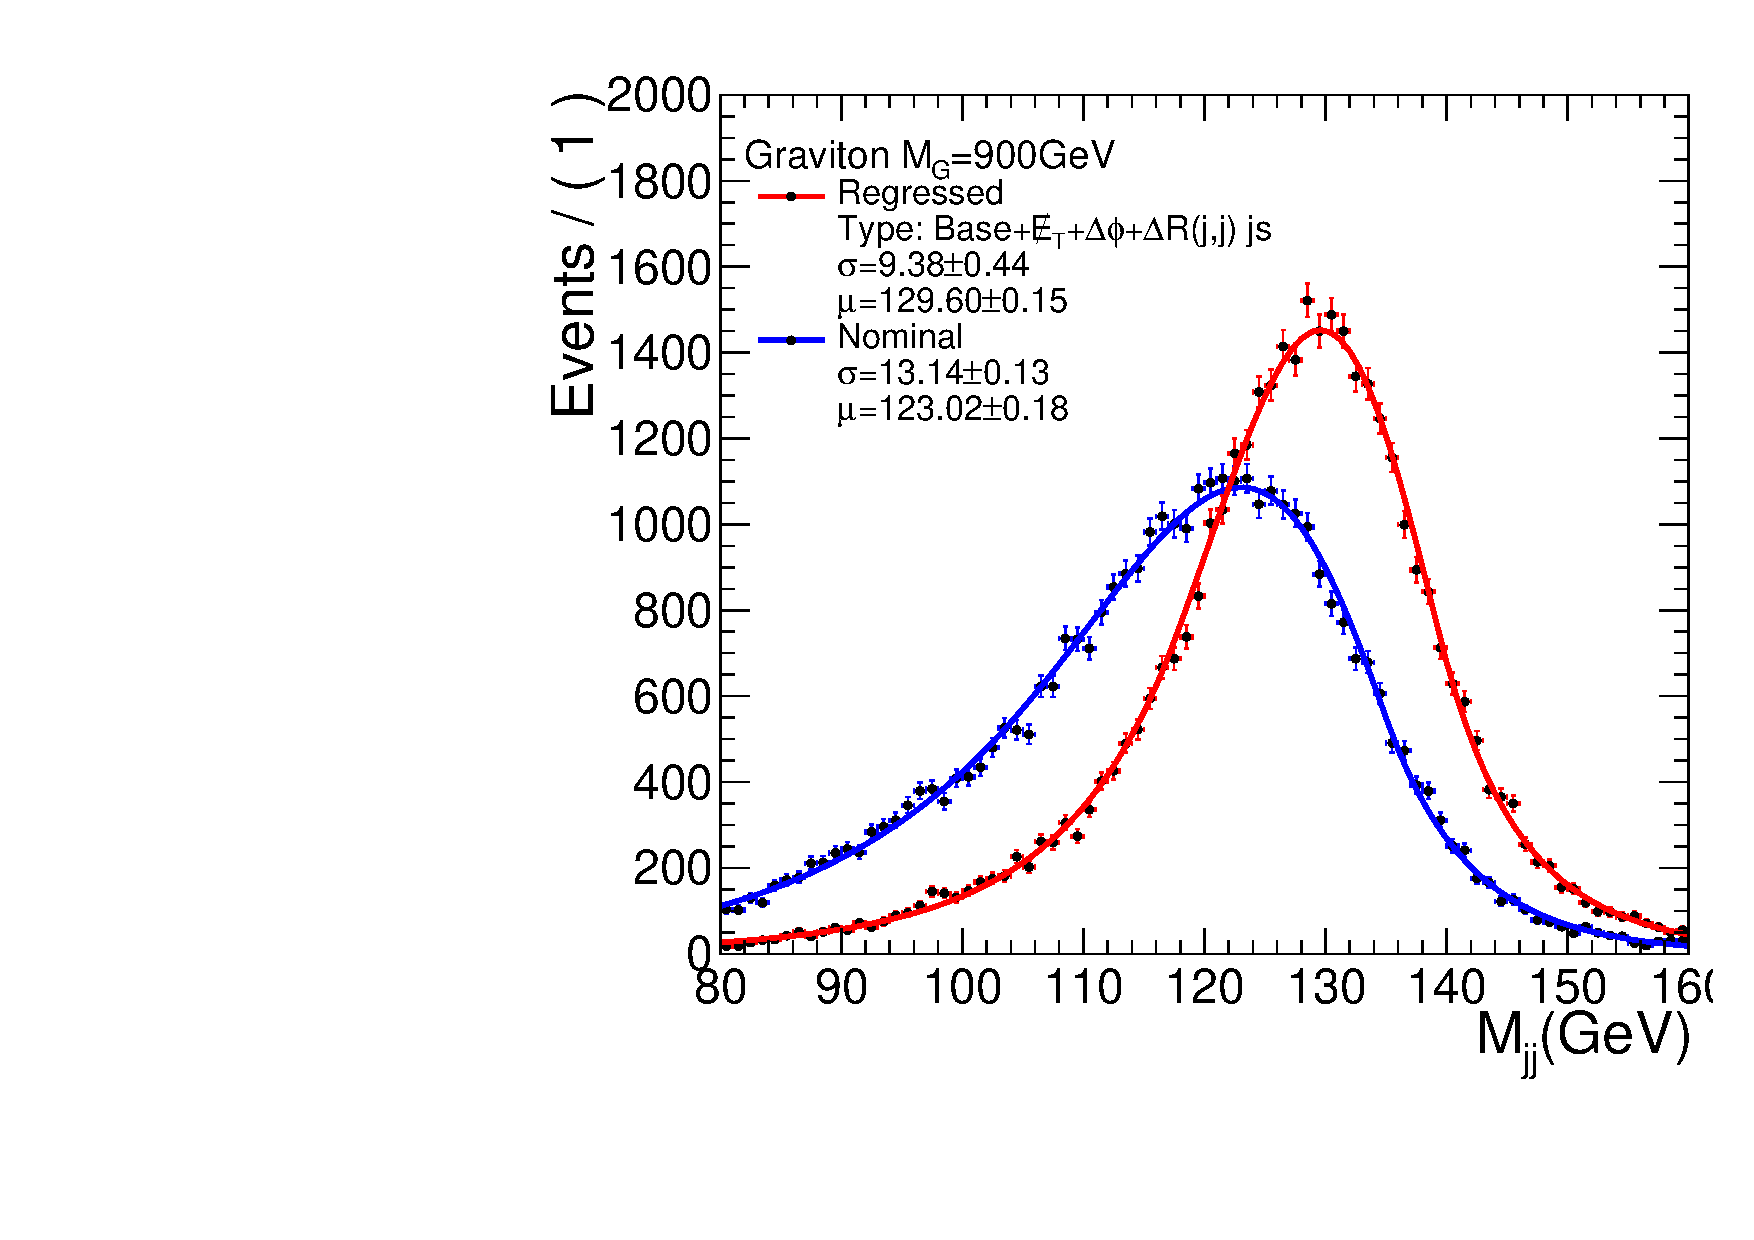
\includegraphics[width=0.35\textwidth]{b-reg/AN_mass900}\hfil
  \caption{$M_{jj}$ distributions from the reco-jets before and after
    the \textbf{full variables with js} regression for $m_G=300\GeV$ signal sample
    (left) and $m_G=900\GeV$ signal sample (right).}
  \label{fig:b-reg-mH-fit-reco}
\end{figure*}

\begin{figure*}[h]
  \centering
  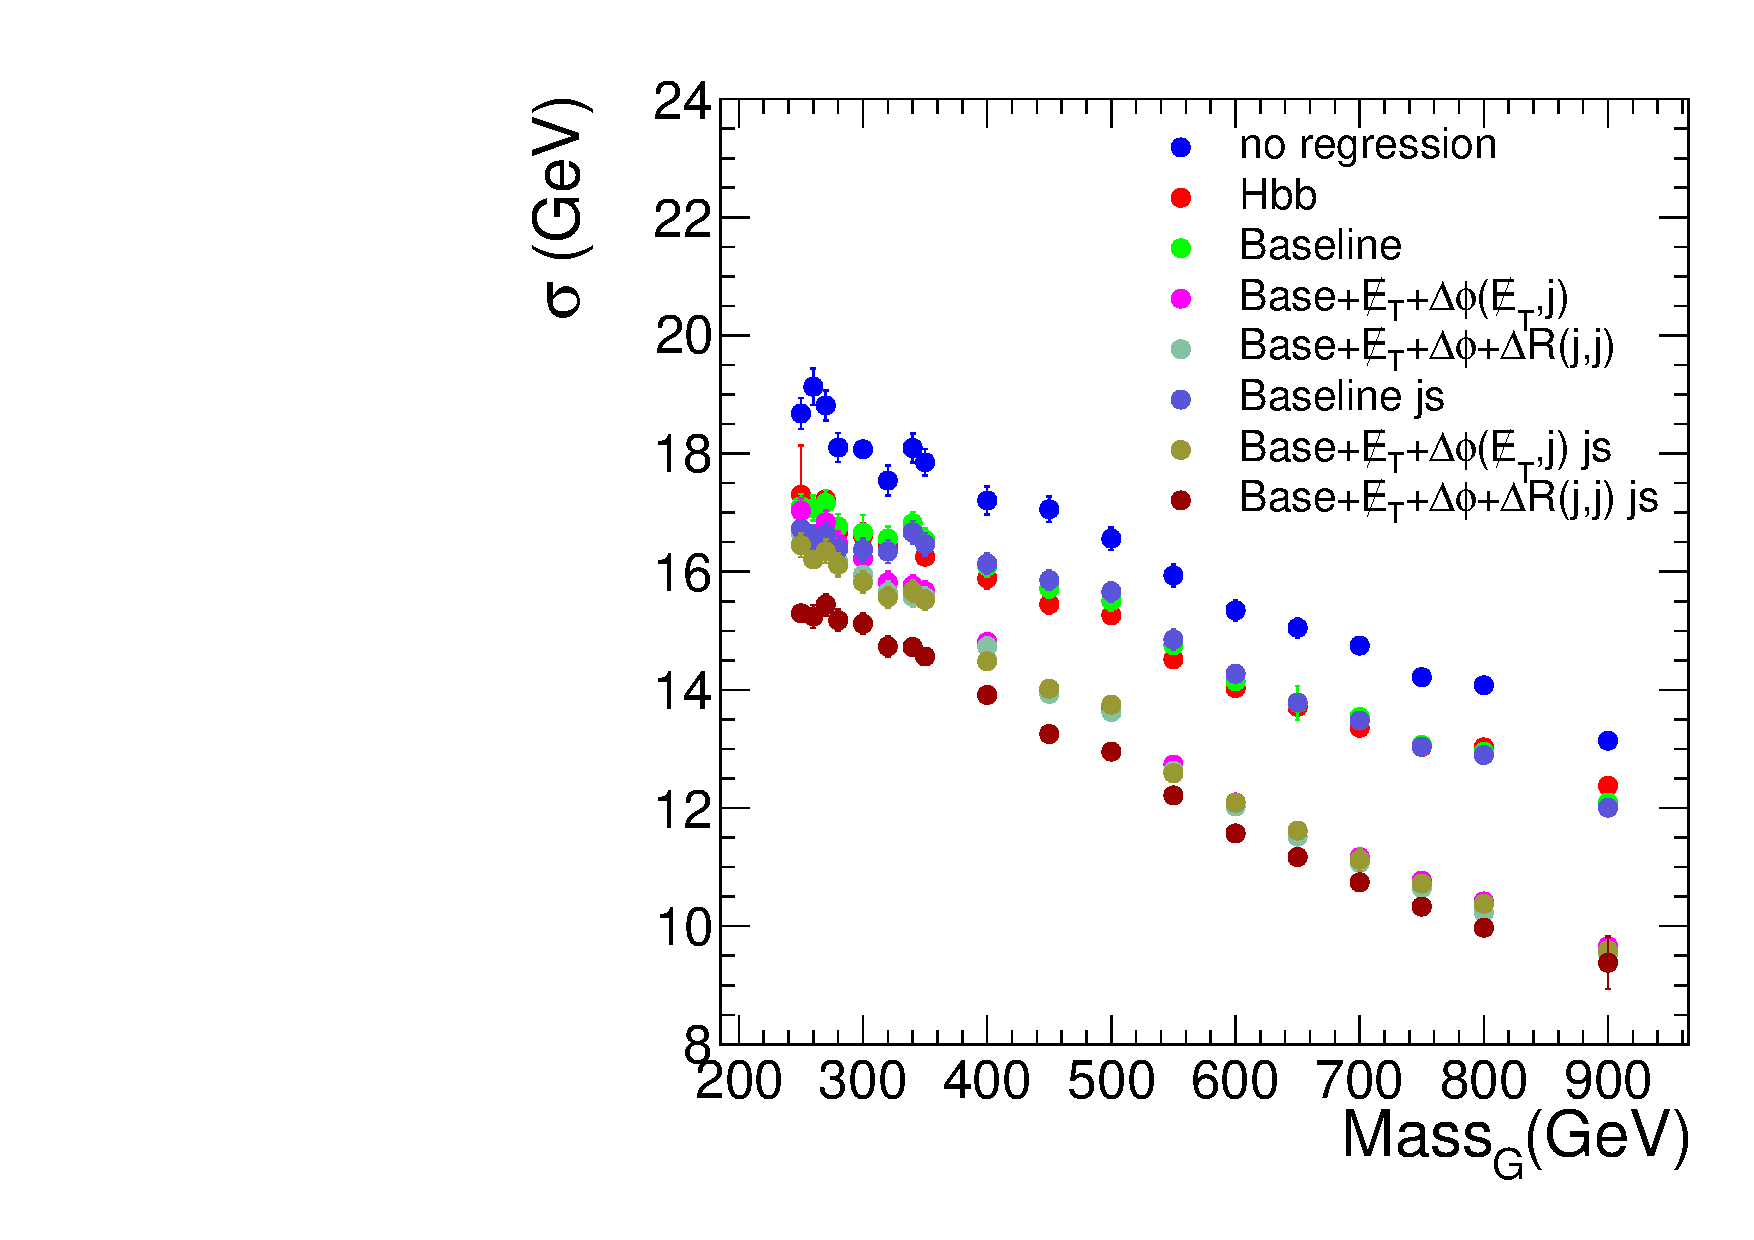
\includegraphics[width=0.35\textwidth]{b-reg/AN_HHbbgg_G_sigma_Mass}\hfil
  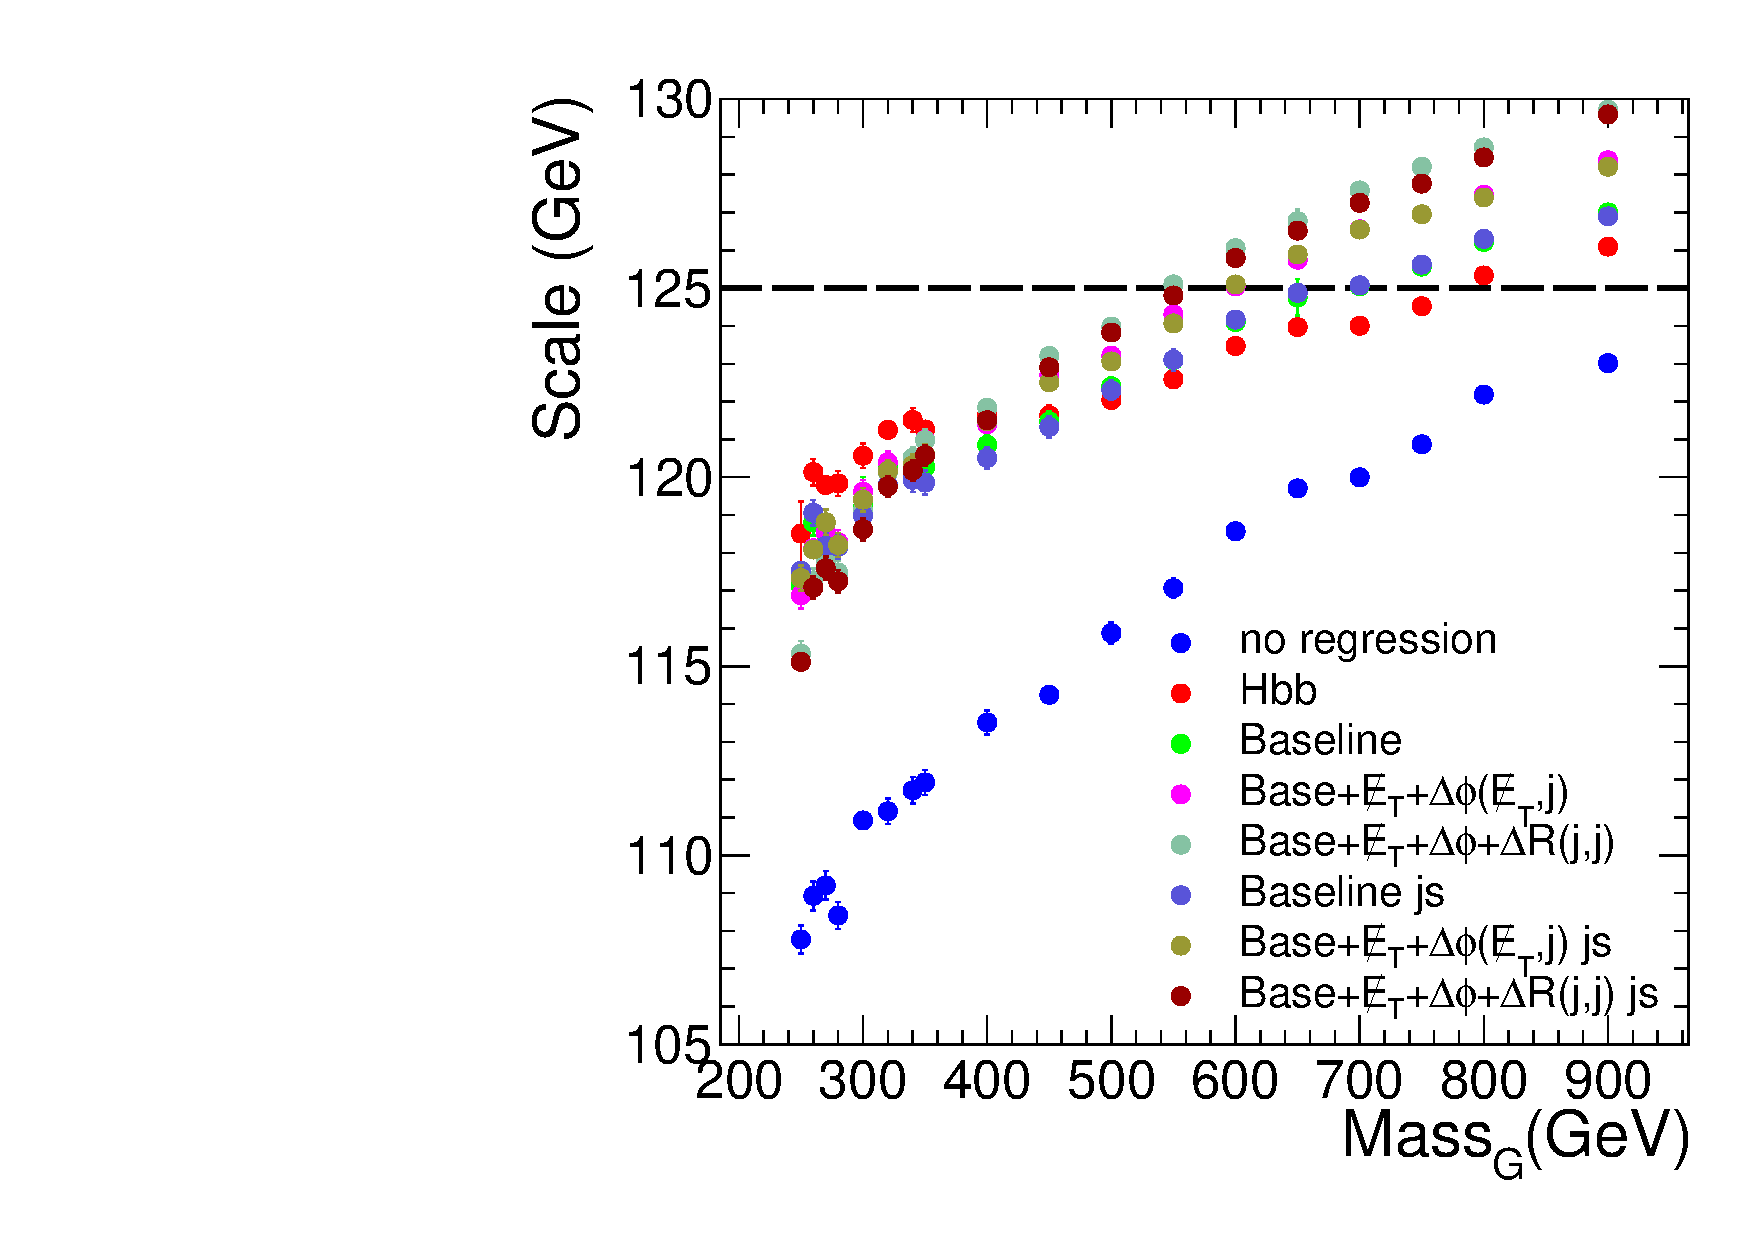
\includegraphics[width=0.35\textwidth]{b-reg/AN_HHbbgg_G_scale_Mass}\hfil
  \caption{Performance plot comparing different regression trainings.}
  \label{fig:b-reg-mH-res}
\end{figure*}


In order to validate the developed regression in data we select events with $\Z\to\ell\ell$ decay which also contain two b-tagged jets. 
It is assumed that a di-jet is recoiled against $\Z$ boson, and therefore the $\PT(jj)$ must balance the $\PT(\ell\ell)$.  
This check was done both in muon and electron channels of \Z boson decay, analyzing \verb|DoubleMuon| and \verb|DoubleElectron| datasets correspondingly, using 2016 data.

In the muon channel the events were selected with an OR of two triggers:
\begin{itemize}
\item \verb|HLT_Mu17_TrkIsoVVL_Mu8_TrkIsoVVL_DZ| and 
\item \verb|HLT_Mu17_TrkIsoVVL_TkMu8_TrkIsoVVL_DZ|. 
\end{itemize}
The reconstructed muons must pass Tight muon ID and Loose PF isolation. 

In the electron channel the \verb|HLT_Ele23_Ele12_CaloIdL_TrackIdL_IsoVL_DZ| trigger was used and
the electrons required to pass MVA ID WP90 selection.  
Further event selection requirements in both channels are: $\PT(\ell_1) > 25\GeV$,
$\PT(\ell_2) > 15\GeV$, $\PT(\ell\ell) > 50\GeV$,
$75<m_{\ell\ell}<105\GeV$, $\Delta R^{min}_{\ell, jet} > 0.4$. The two
jets in the event must pass Loose PF ID selection, Medium PU jet ID,
tagged as b-jets with CSVv2 Medium WP, and have $\PT>20\GeV$,
$|\eta|<2.4$.

\begin{figure*}[thb]
  \centering
  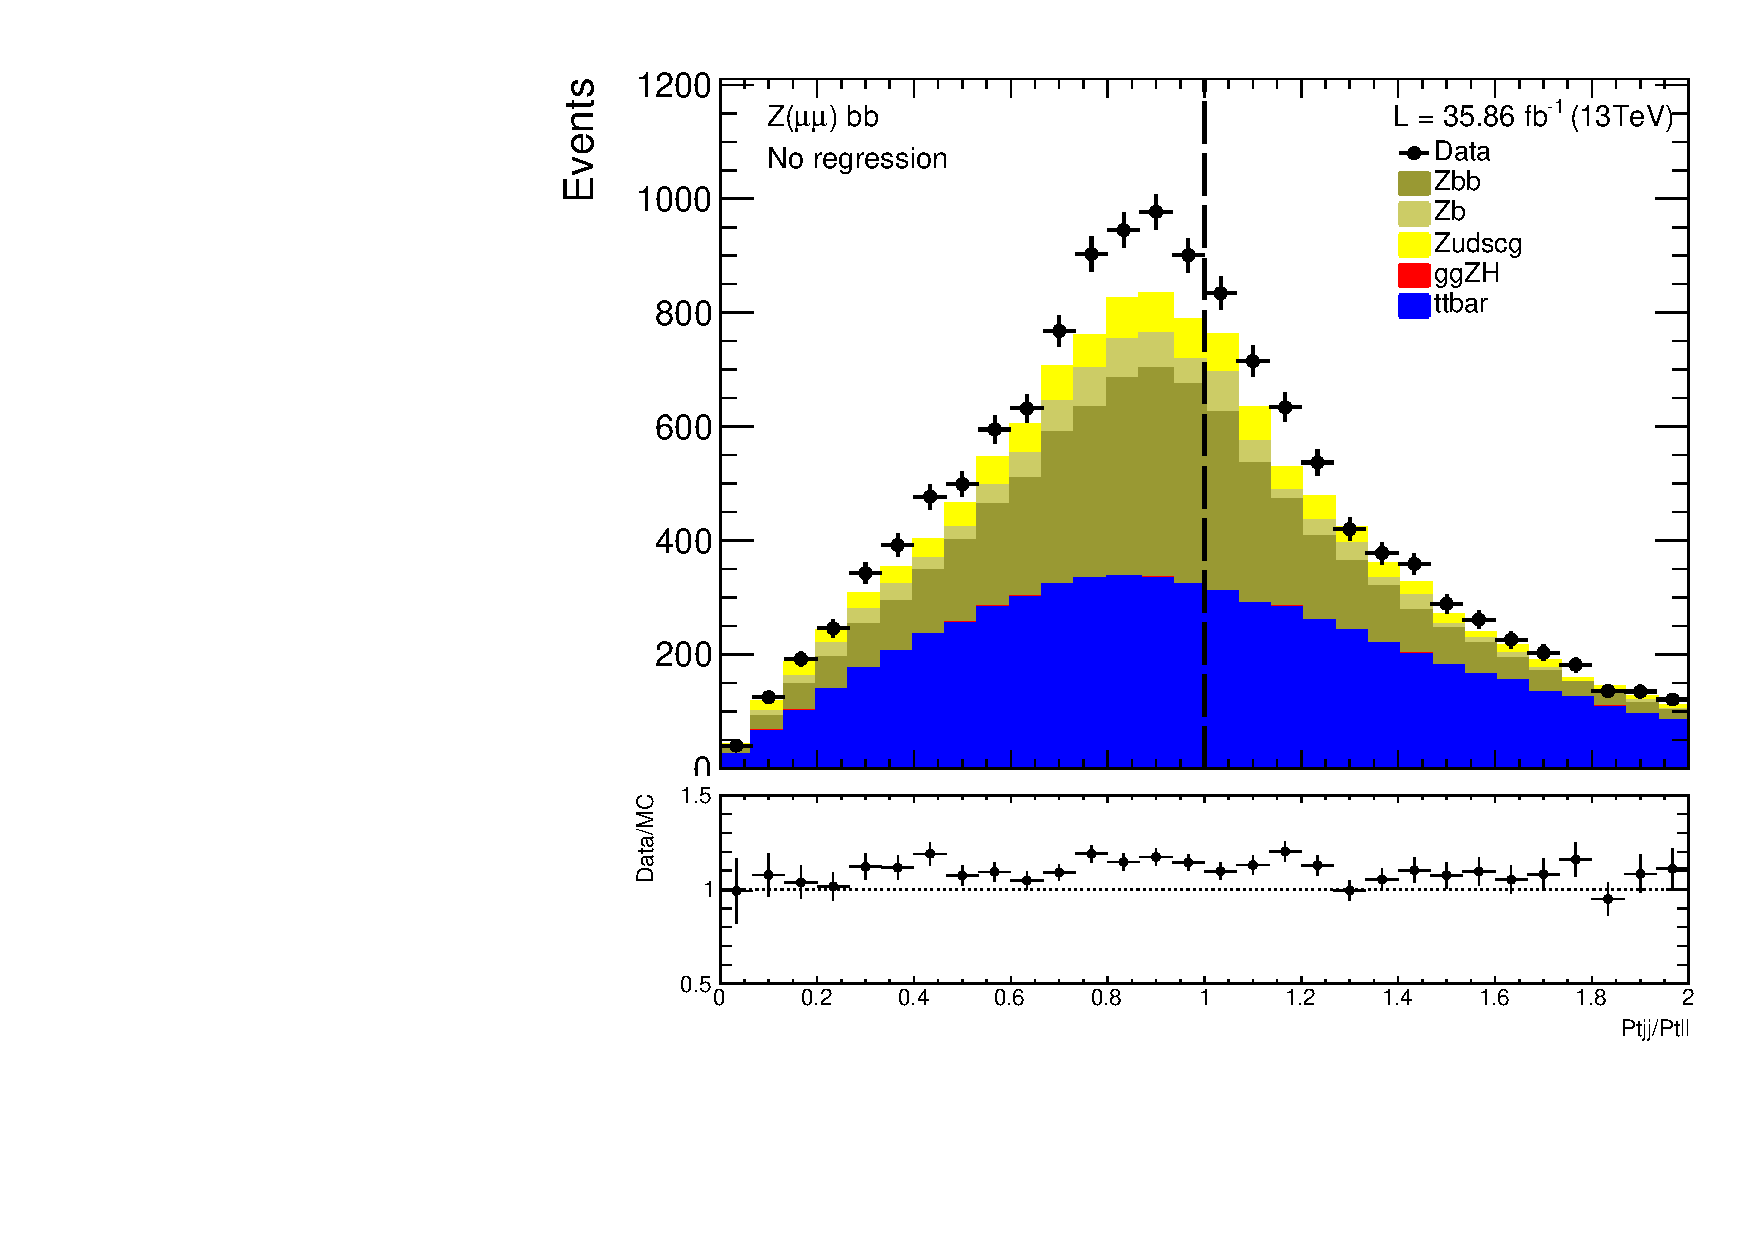
\includegraphics[width=0.32\textwidth]{b-reg/Vali_Data_MC_no_reg__PtBalance_mu_Medium}\hfil
  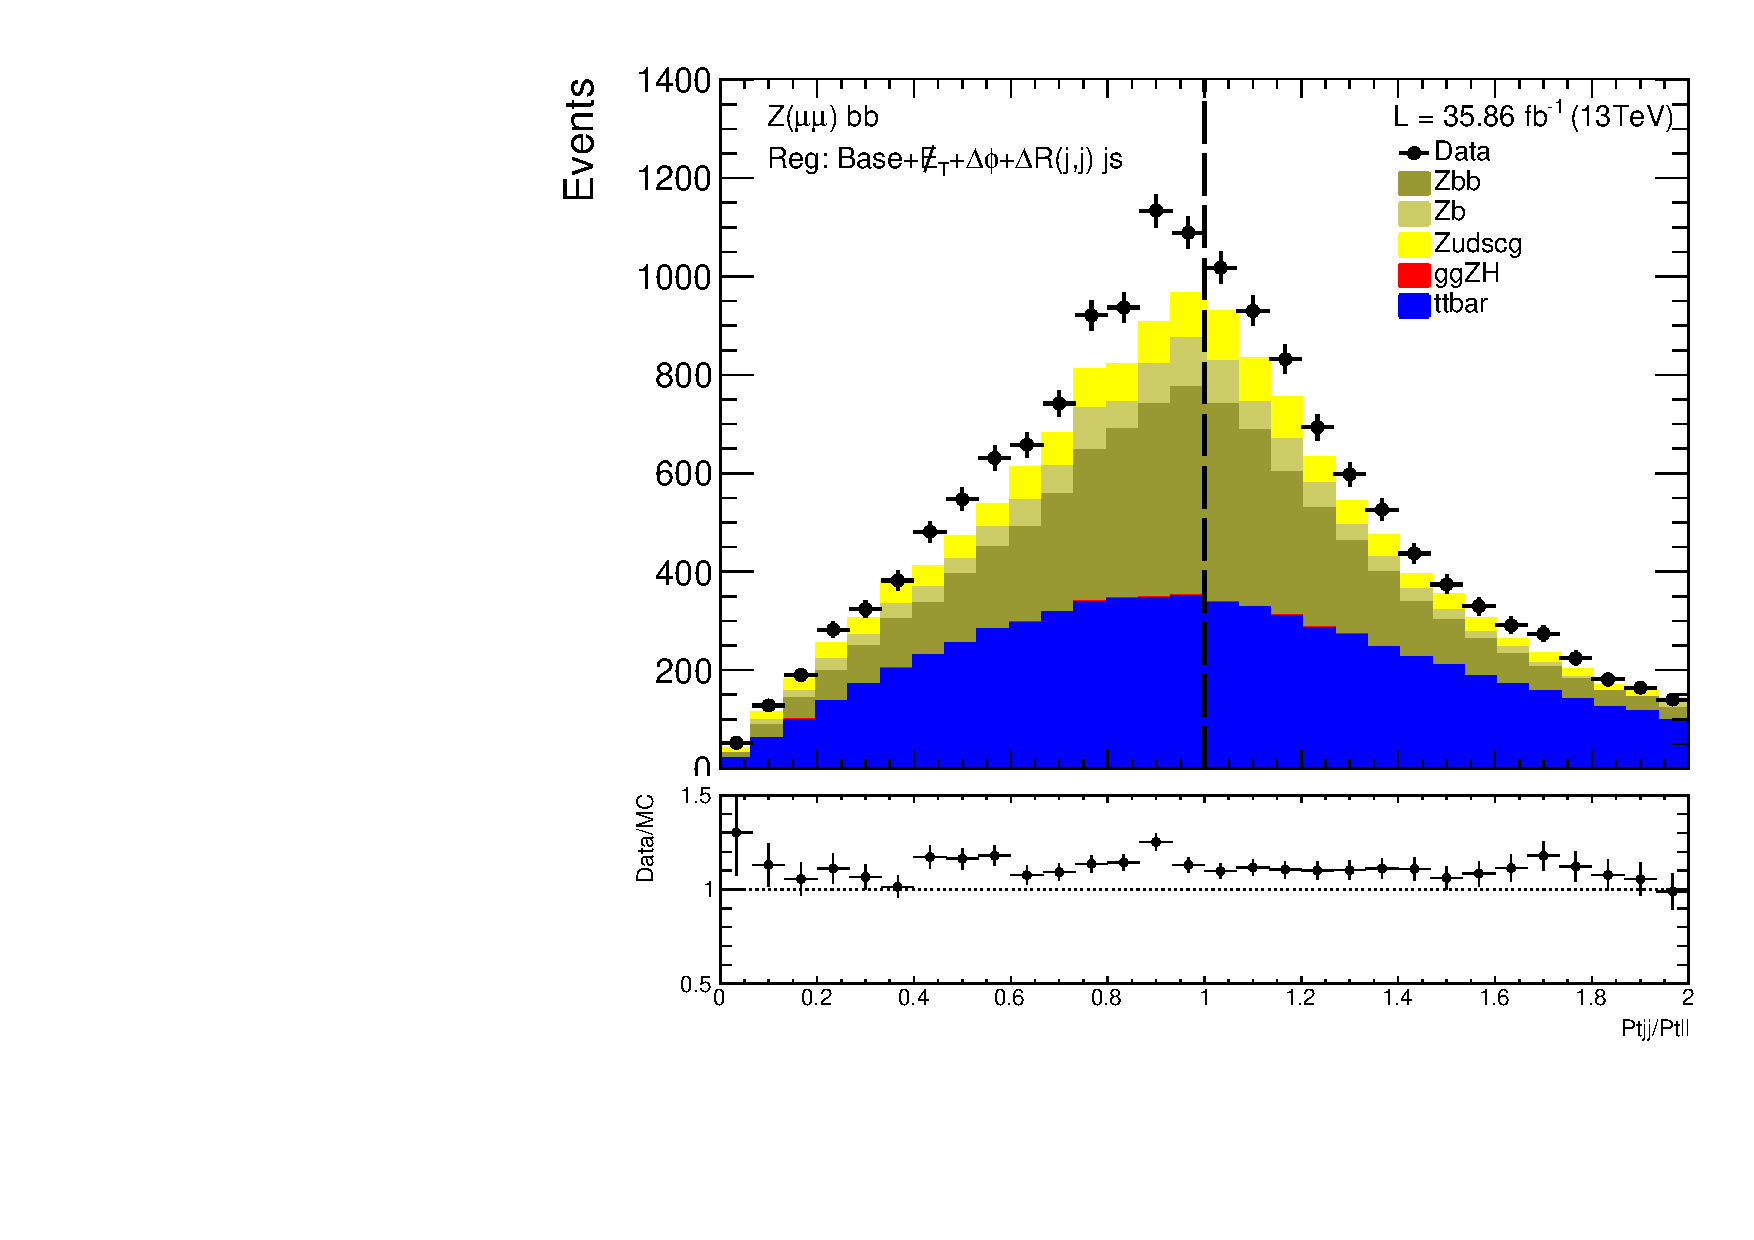
\includegraphics[width=0.32\textwidth]{b-reg/Vali_Data_MC_jet_15plus3_js_2_27__PtBalance_mu_Medium}\hfil
  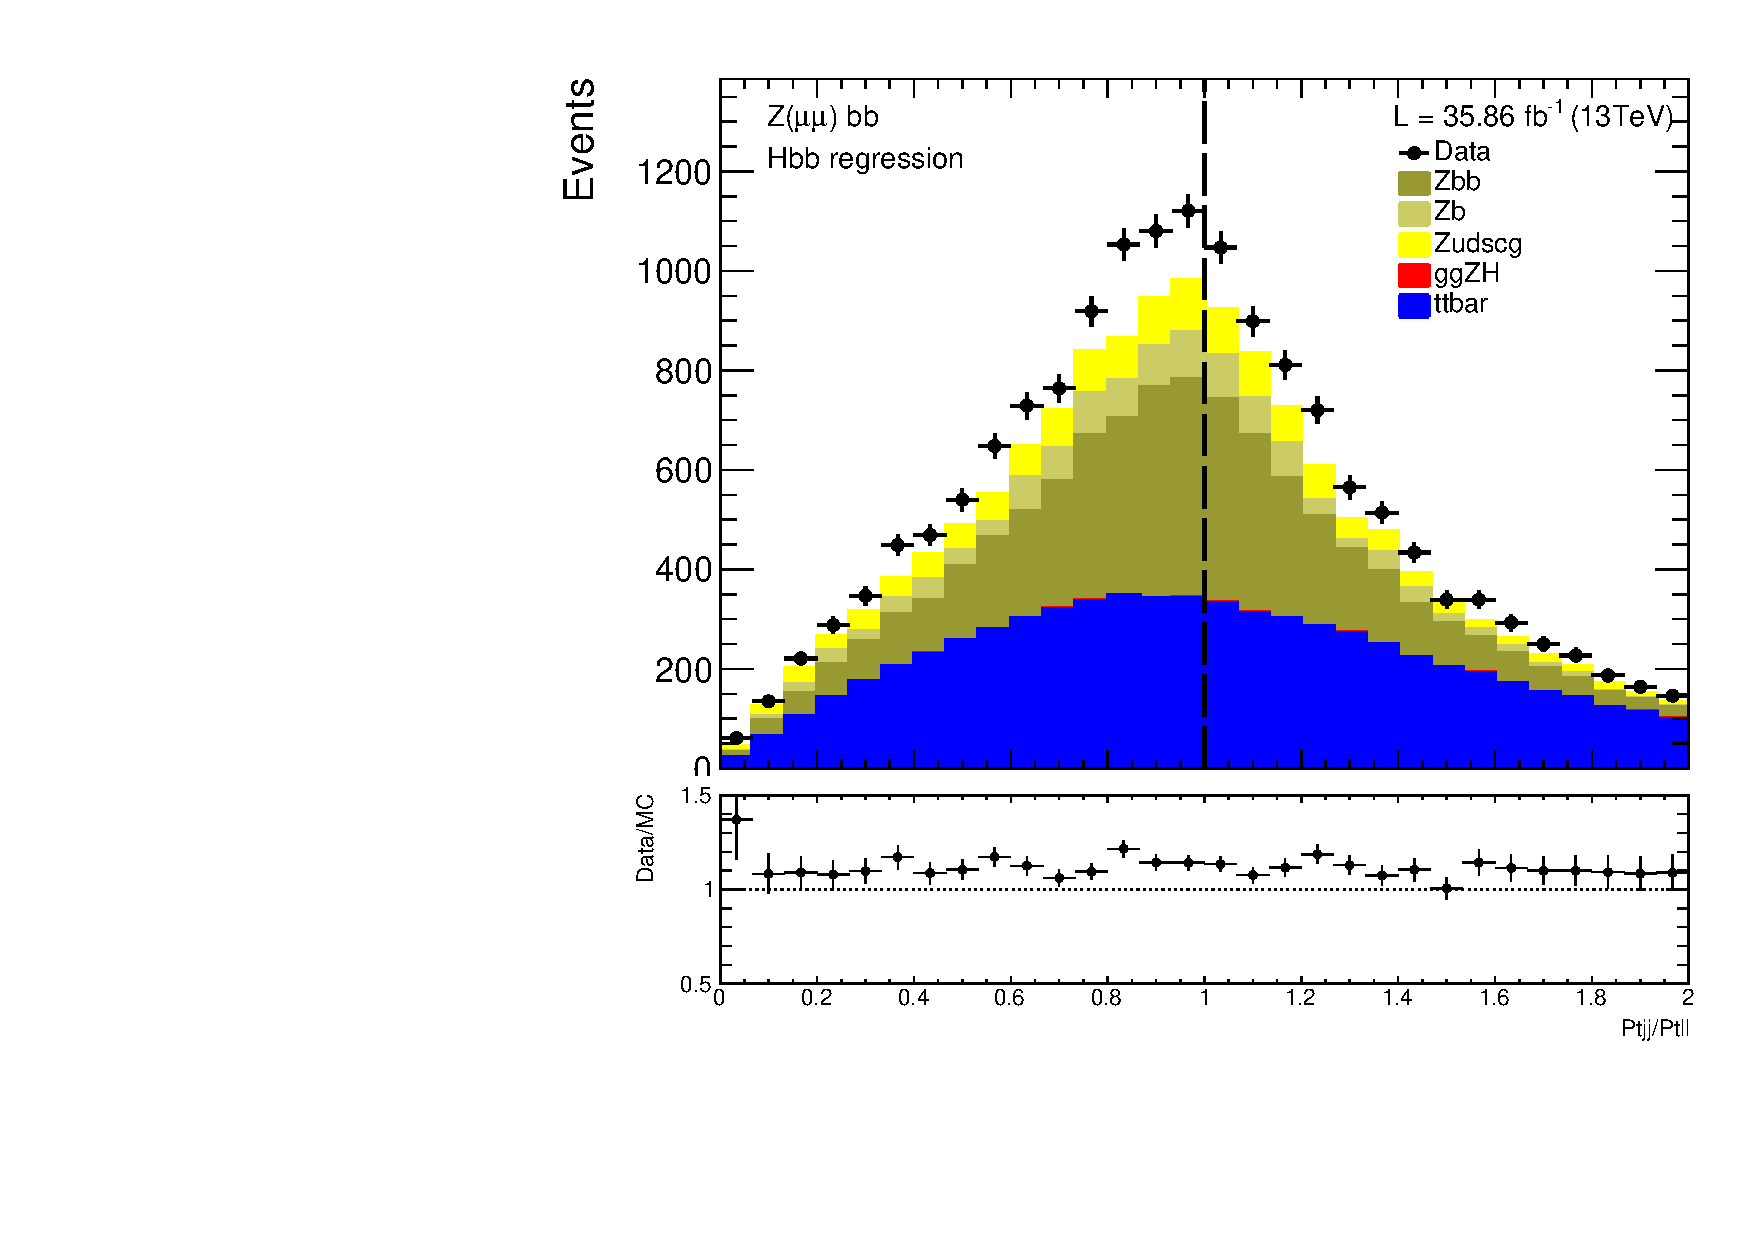
\includegraphics[width=0.32\textwidth]{b-reg/Vali_Data_MC_jet_Hbb__PtBalance_mu_Medium}\hfil\\
  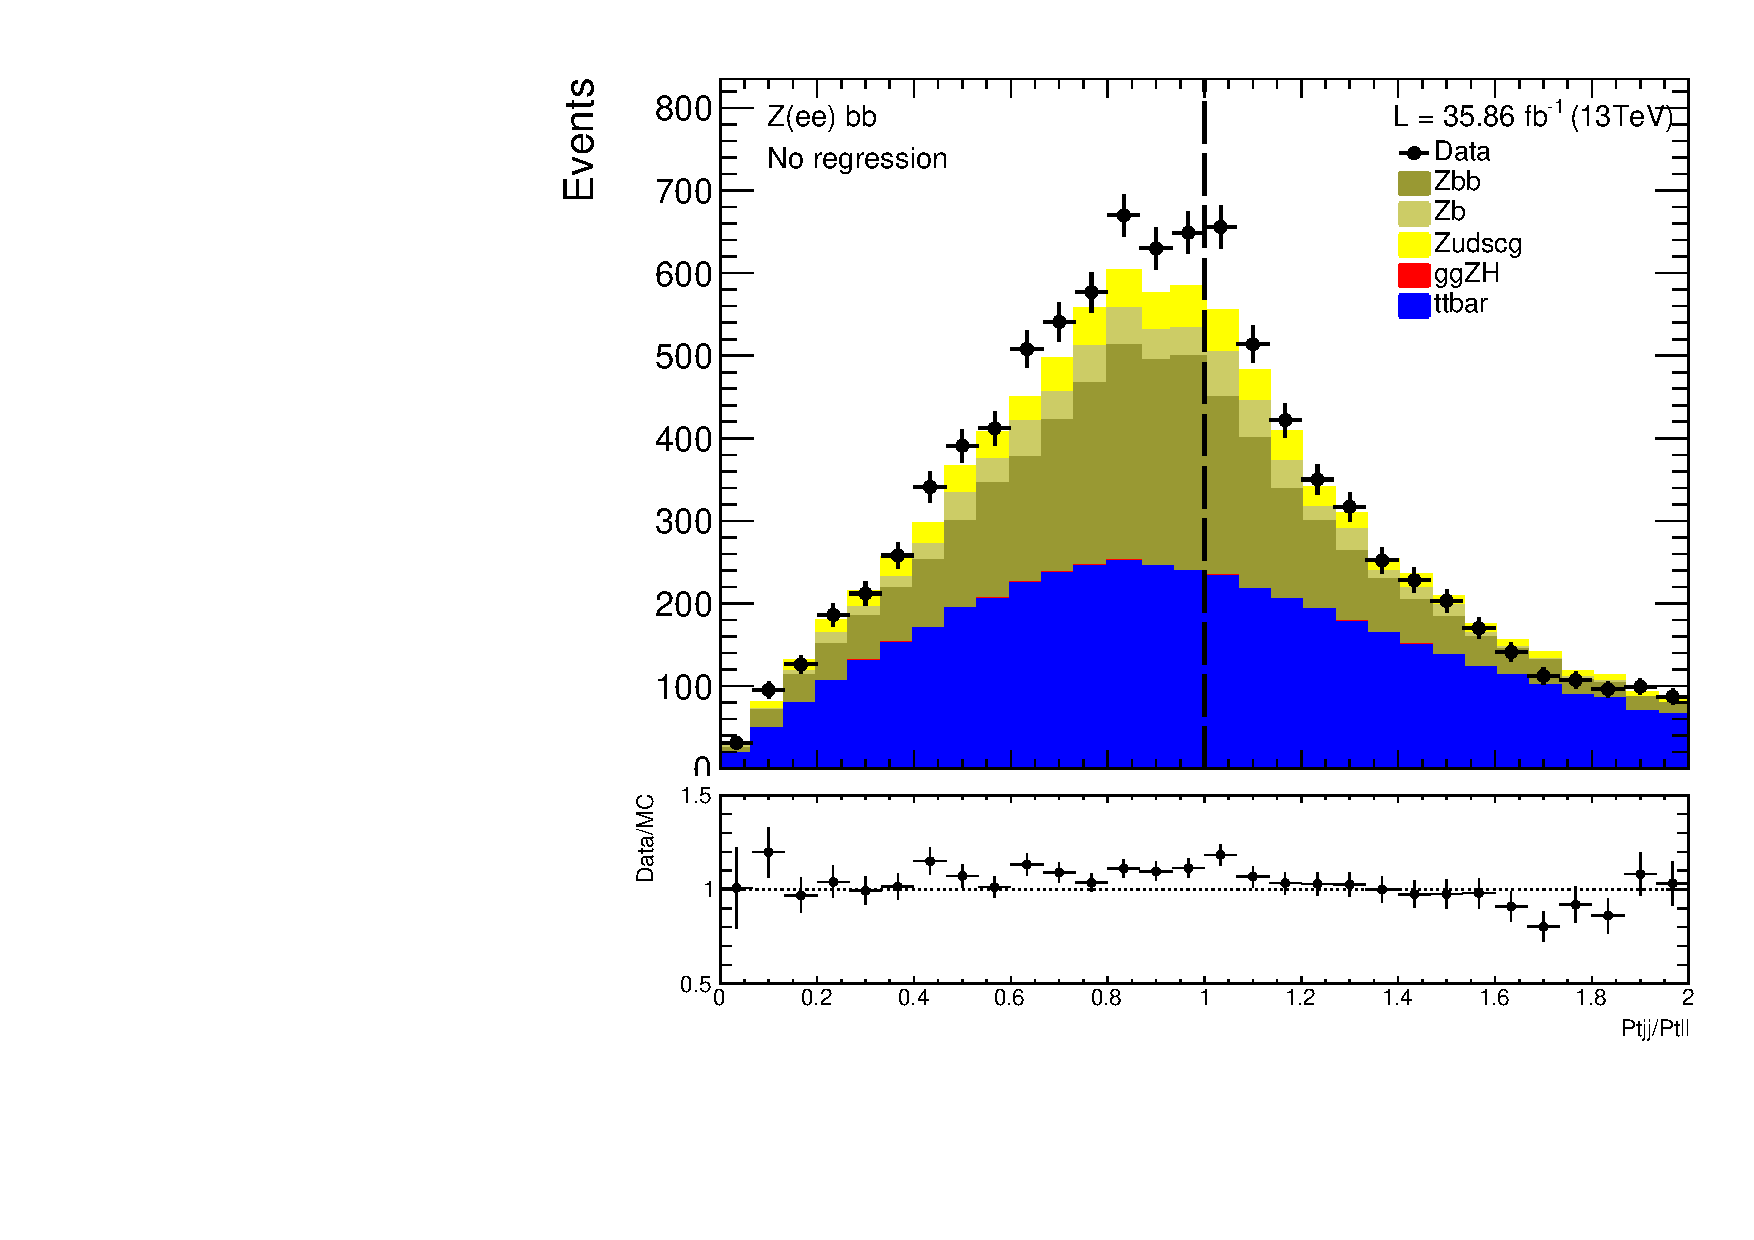
\includegraphics[width=0.32\textwidth]{b-reg/Vali_Data_MC_no_reg__PtBalance_ele_Medium}\hfil
  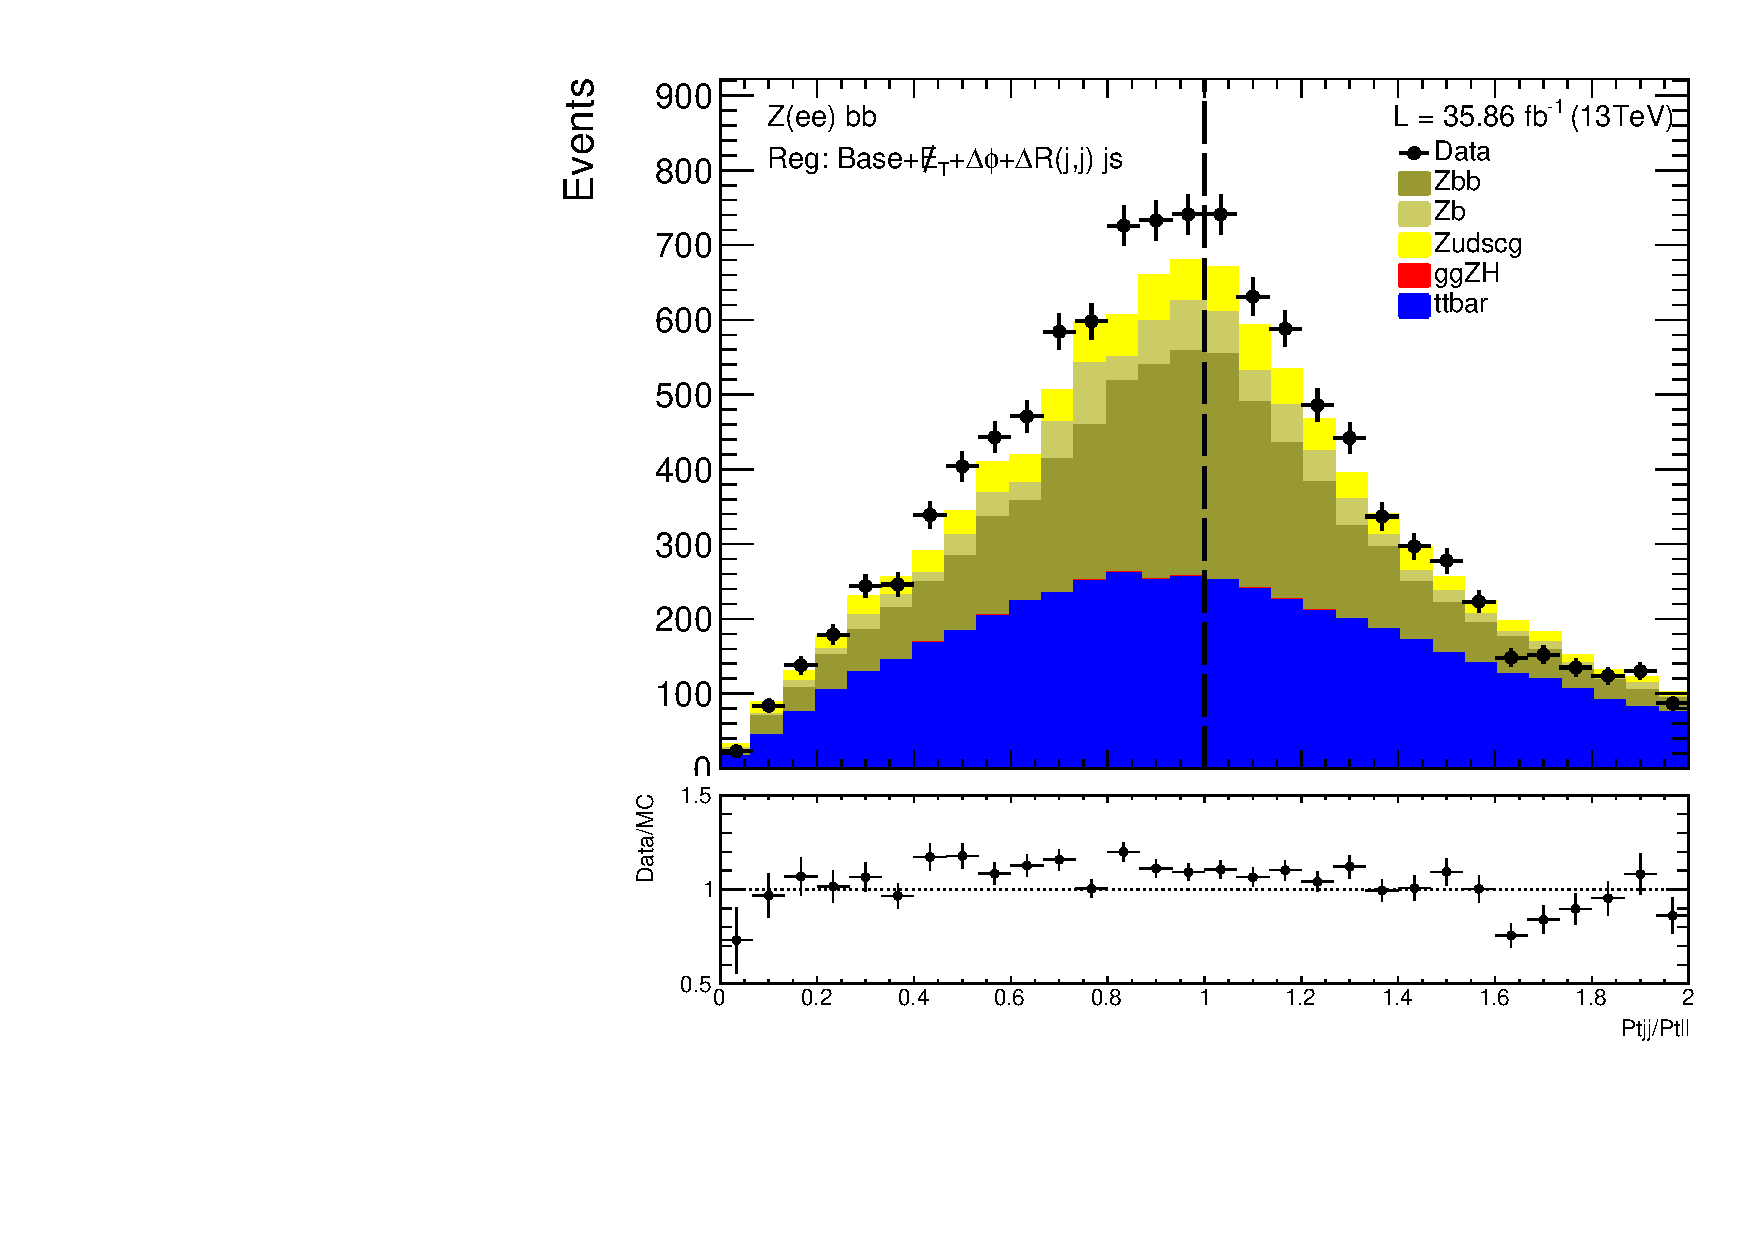
\includegraphics[width=0.32\textwidth]{b-reg/Vali_Data_MC_jet_15plus3_js_2_27__PtBalance_ele_Medium}\hfil
  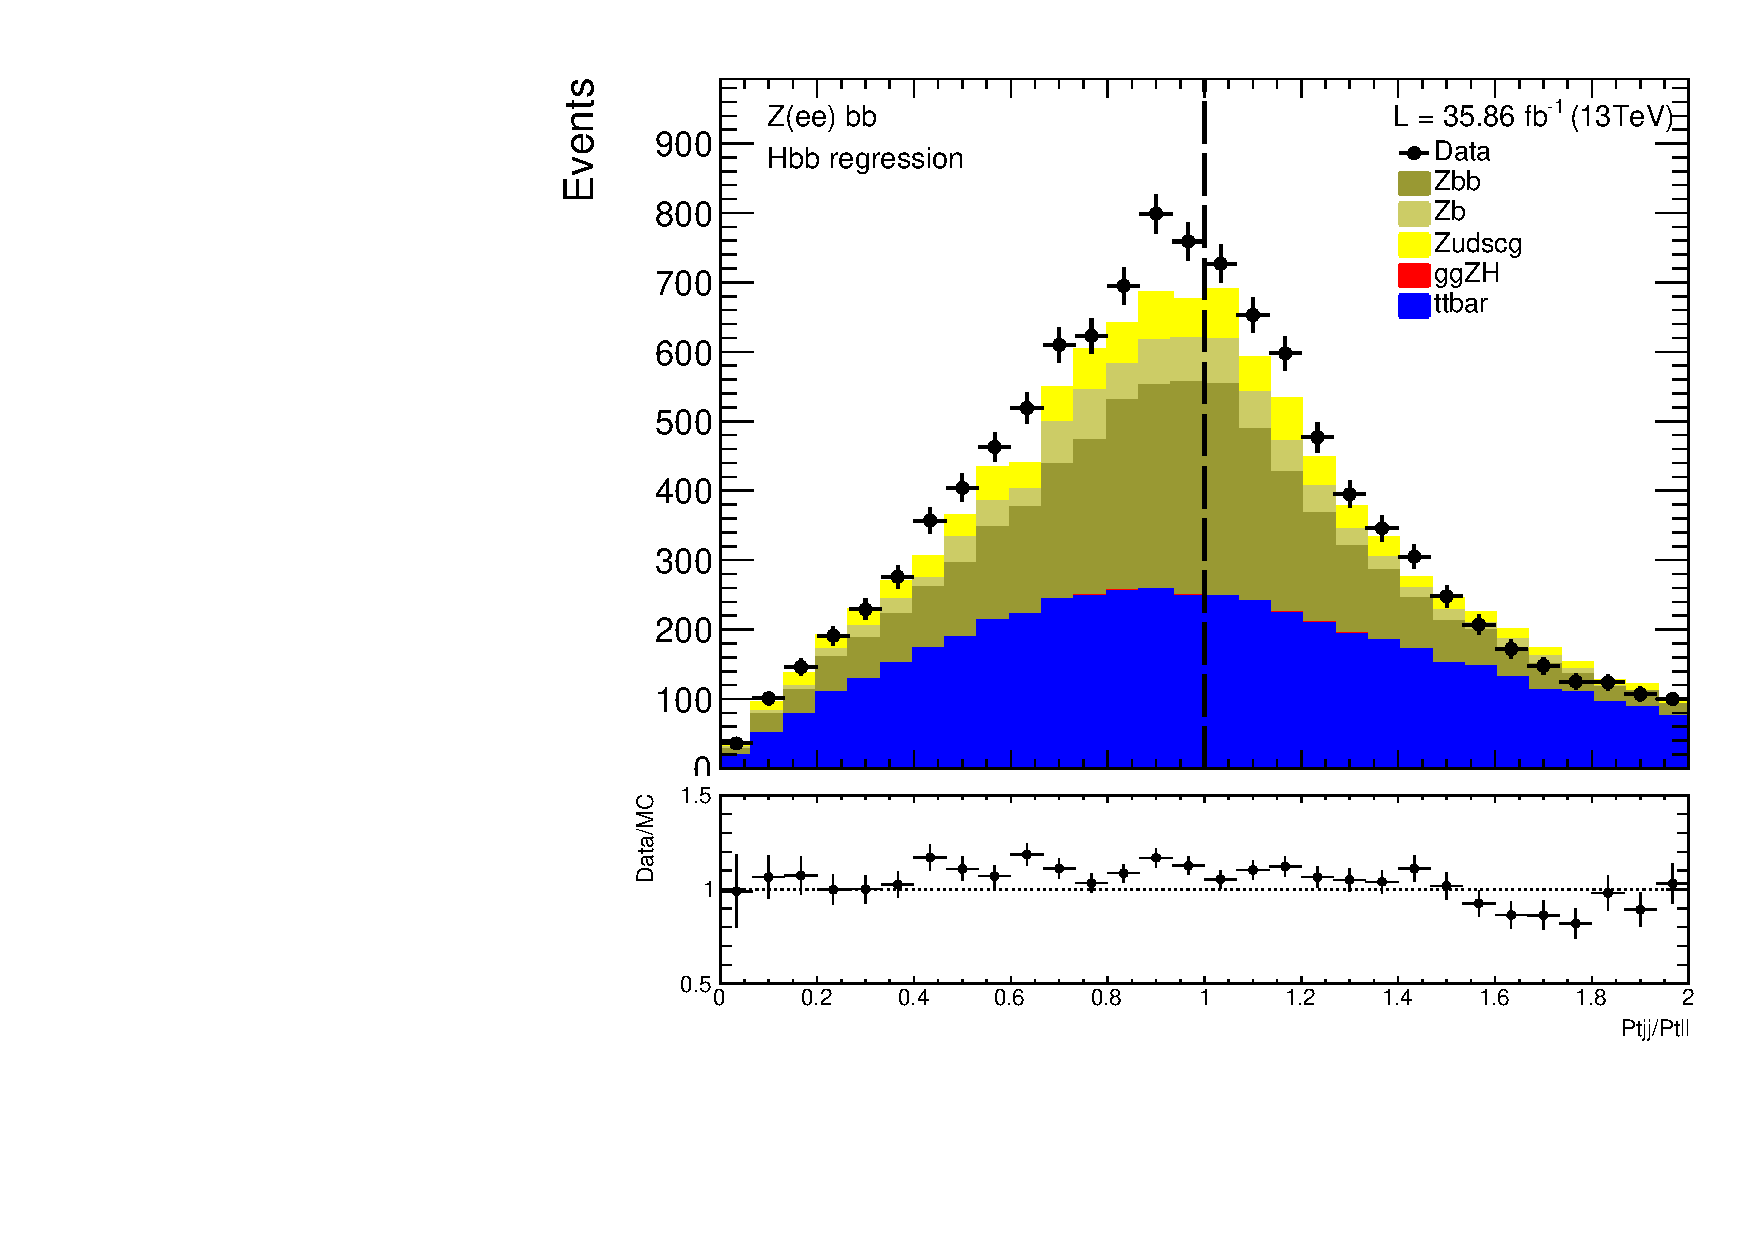
\includegraphics[width=0.32\textwidth]{b-reg/Vali_Data_MC_jet_Hbb__PtBalance_ele_Medium}\hfil\\
  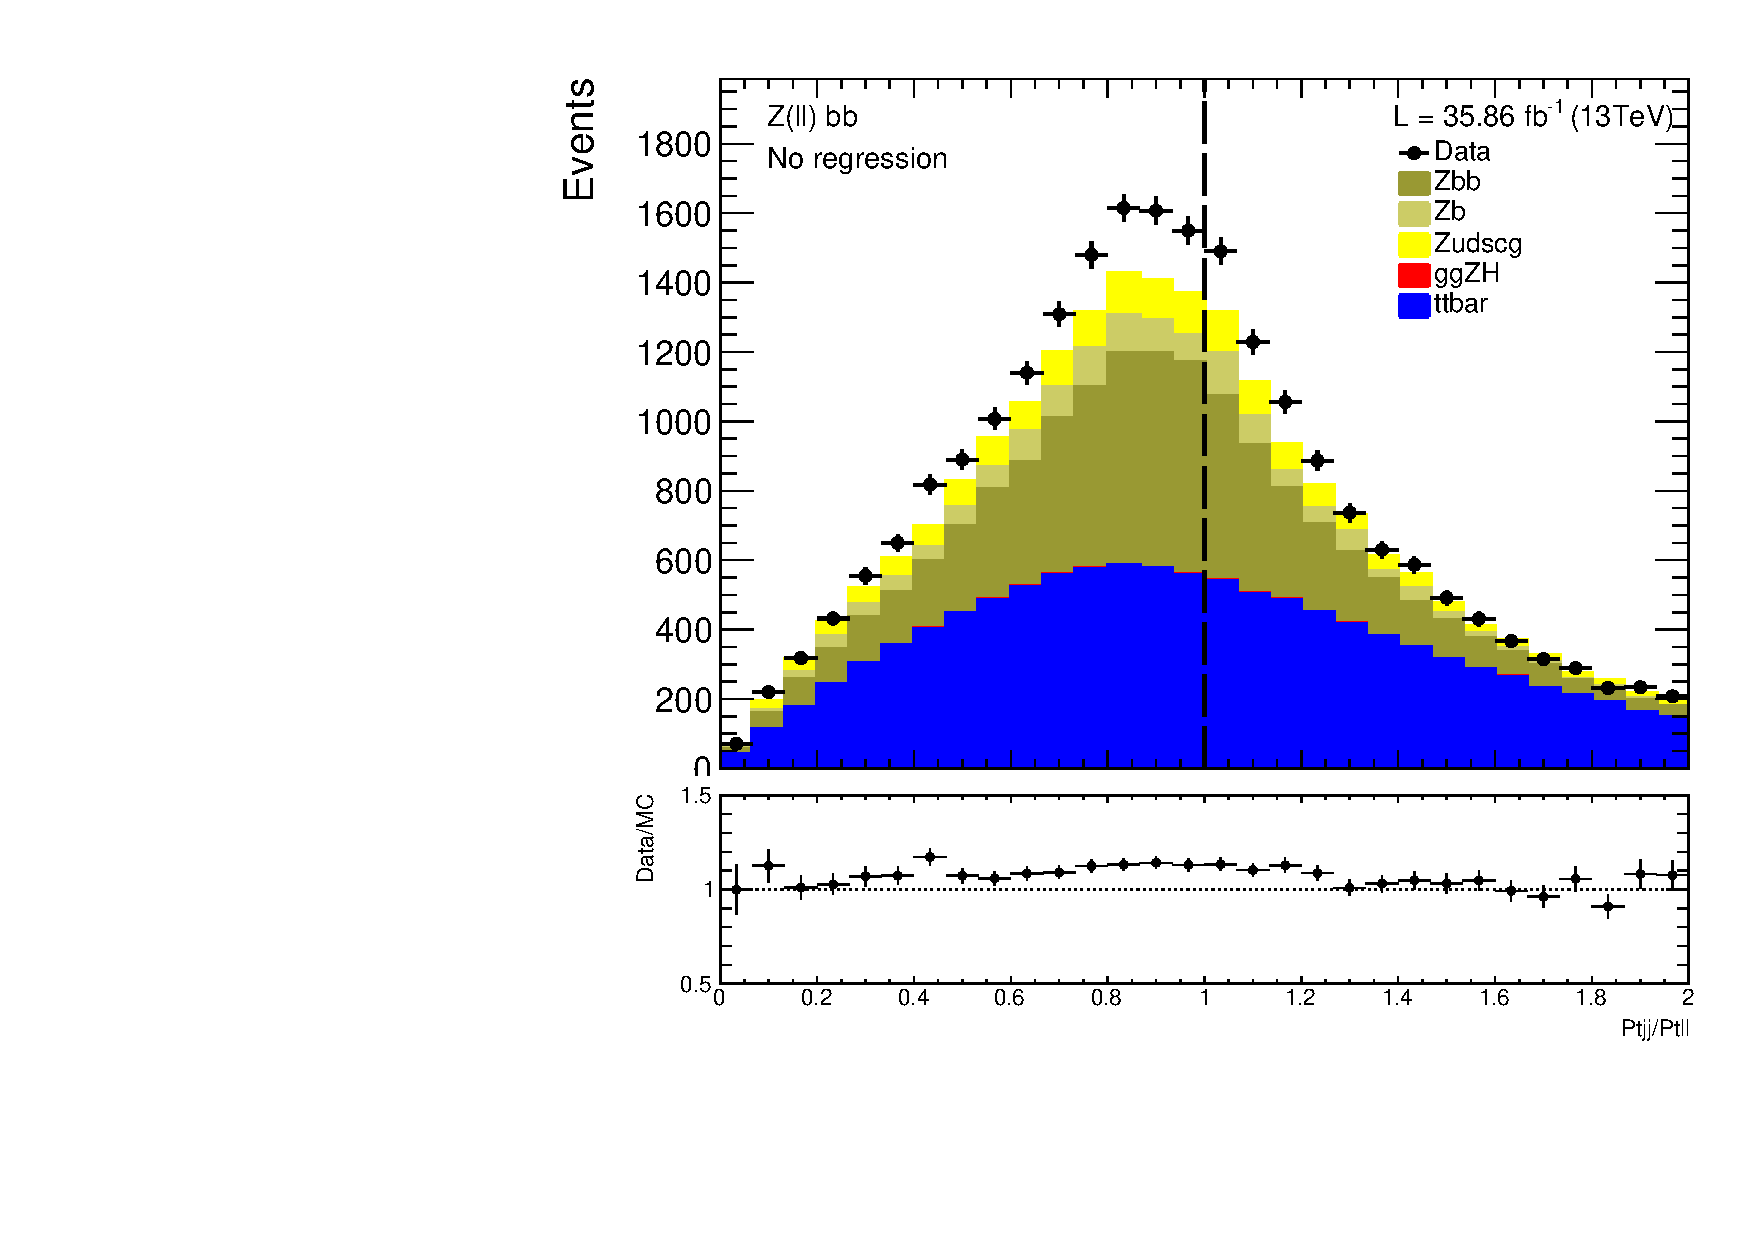
\includegraphics[width=0.32\textwidth]{b-reg/Vali_Data_MC_no_reg__PtBalance_all_Medium}\hfil
  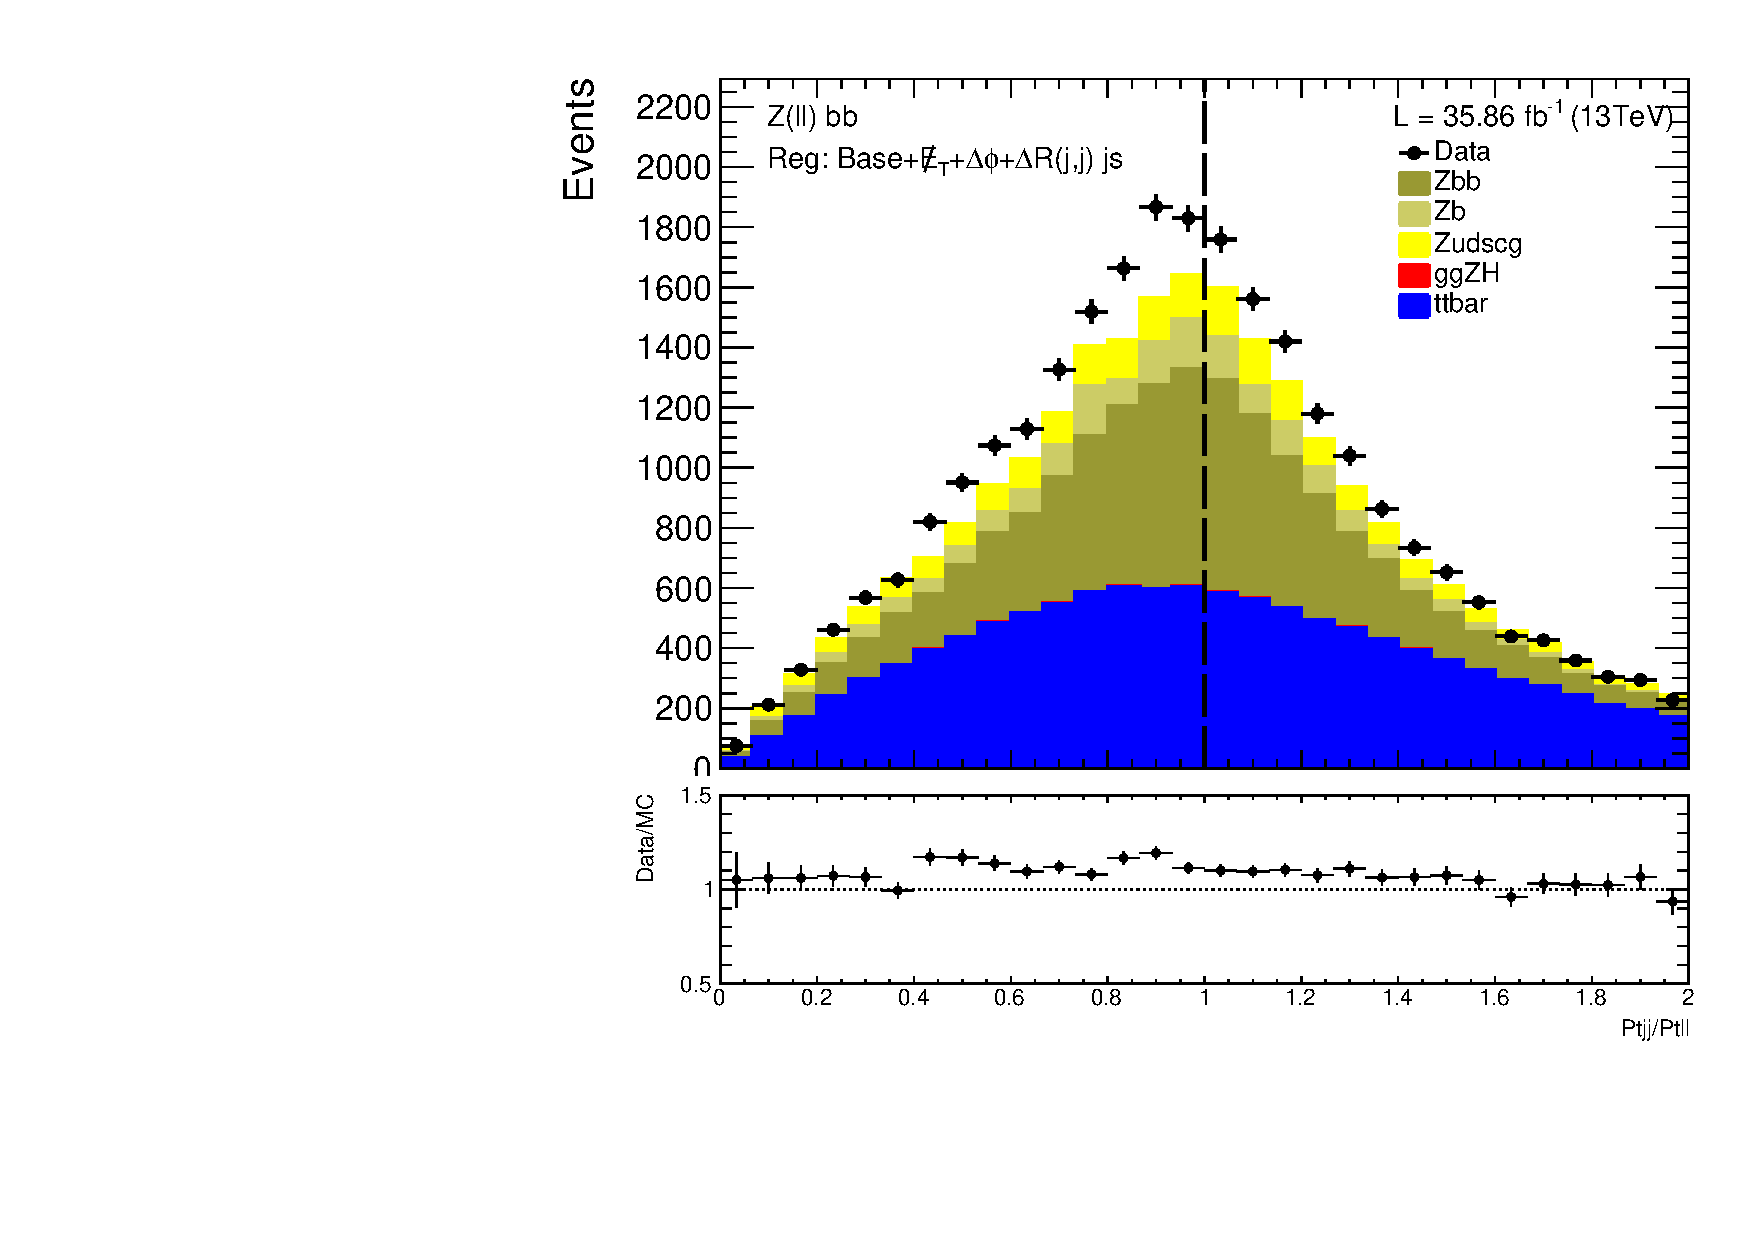
\includegraphics[width=0.32\textwidth]{b-reg/Vali_Data_MC_jet_15plus3_js_2_27__PtBalance_all_Medium}\hfil
  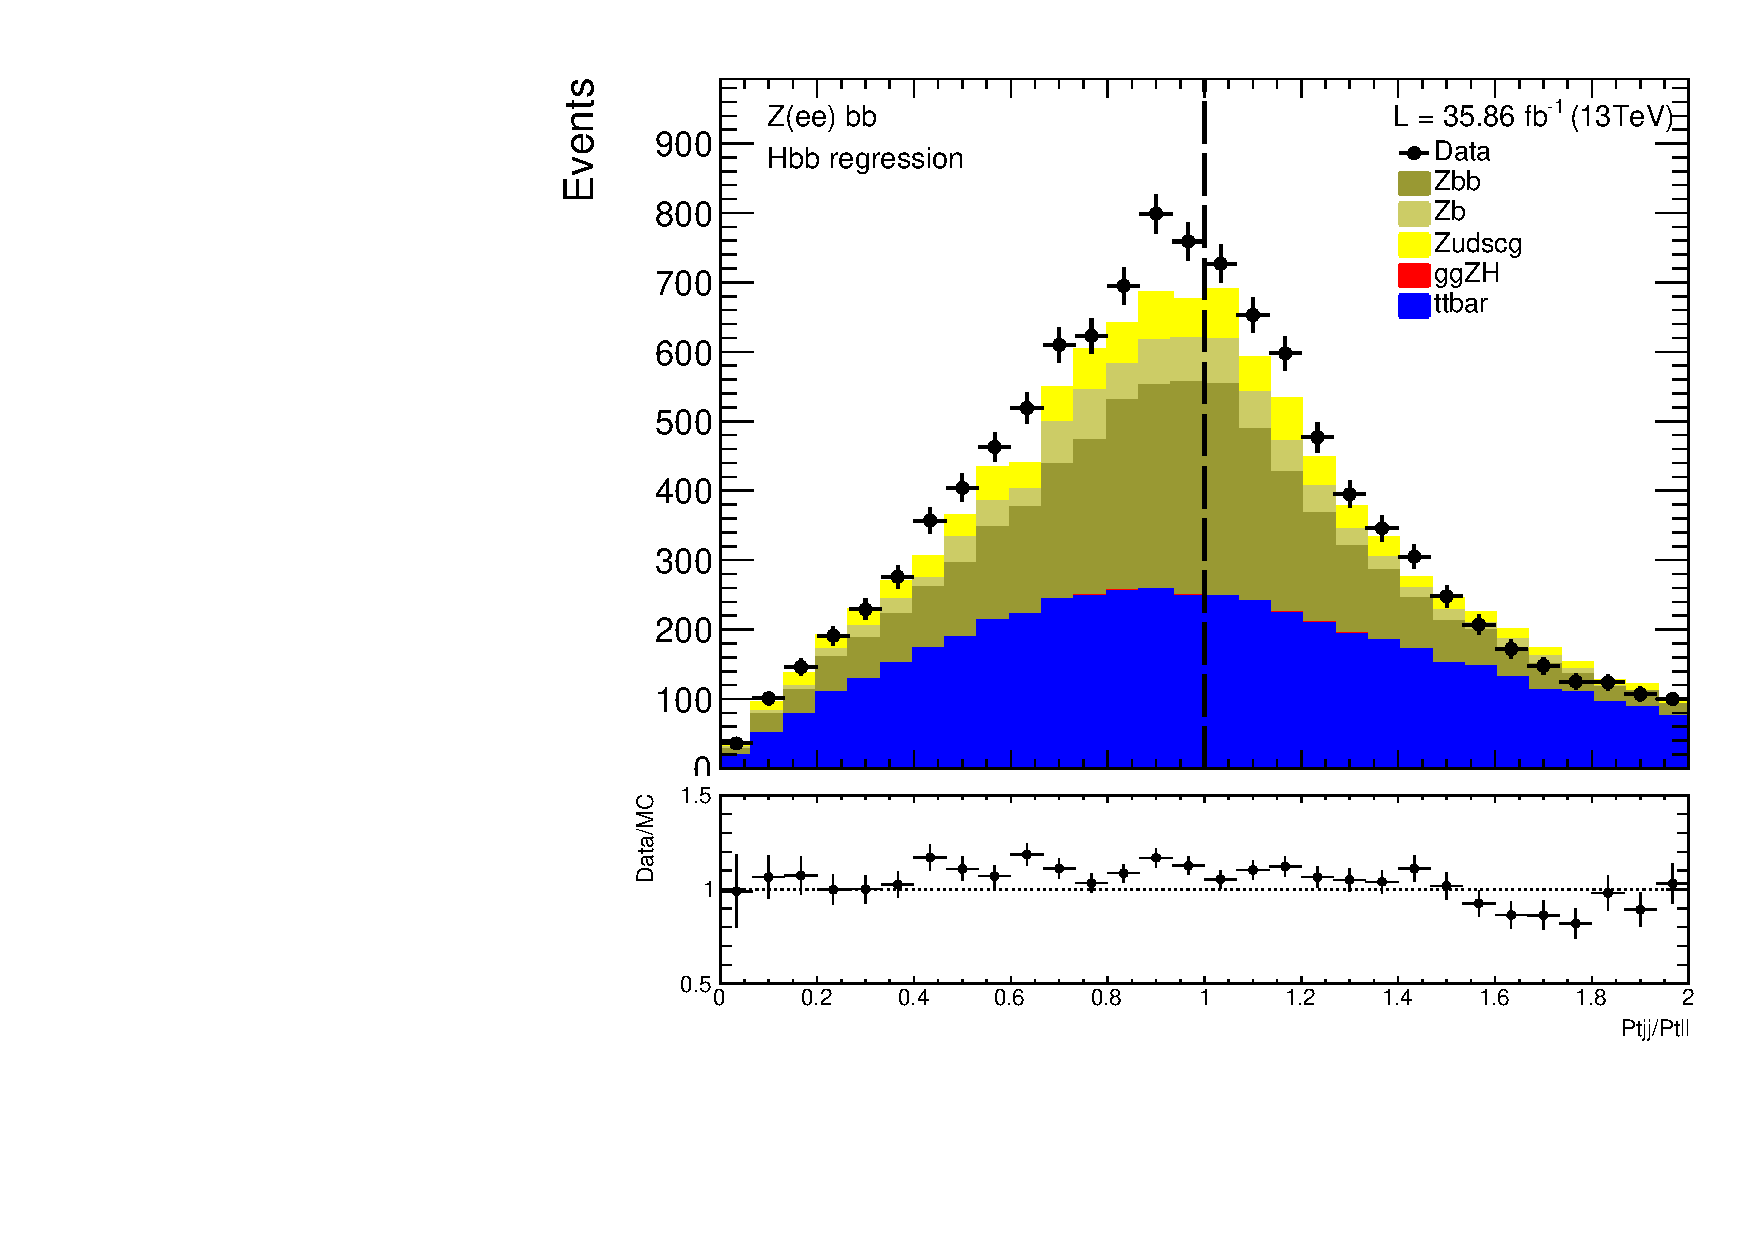
\includegraphics[width=0.32\textwidth]{b-reg/Vali_Data_MC_jet_Hbb__PtBalance_ele_Medium}\hfil\\
  \caption{Pt balance (ratio) of the di-jet and di-lepton. On the left
    are the distributions without regression, in the center - using
    \textbf{full 15+3var js} training and on the right - using
    \textbf{Hbb} regression.  Top plots are for muon channel, middle
    for electron channel and bottom is the combination (sum) of the
    two.}
  \label{fig:vali-pt}
\end{figure*}

Figure \ref{fig:vali-pt} shows the mentioned $\PT$-balance
distributions, $\PT^{jj}/\PT^{\ell\ell}$.  The data is compared to the
MC predictions. It can be seen that before any regression is applied to avoid over training.
(left plots) the peak of the ratio distribution is below one. With the
regression applied the peak moves to 1 for both our \textbf{full variables with js}
 training (center) and the one from \textbf{Hbb} (right). The
trend is the same in data and MC.  This indicates that the regression
does indeed brings the $\PT$ of the $b$-jets closer to their true
values.

Similarly, figure~\ref{fig:vali-Mjj} shows the mass distributions,
$m_{jj}$, before and after regression. These figures indicate that
$m_{jj}$ is not distorted in any bad way, no artificial peaks are
created. This ensures us that the background distributions in our
analysis signal region will not be distorted either.


\begin{figure*}[thb]
  \centering
  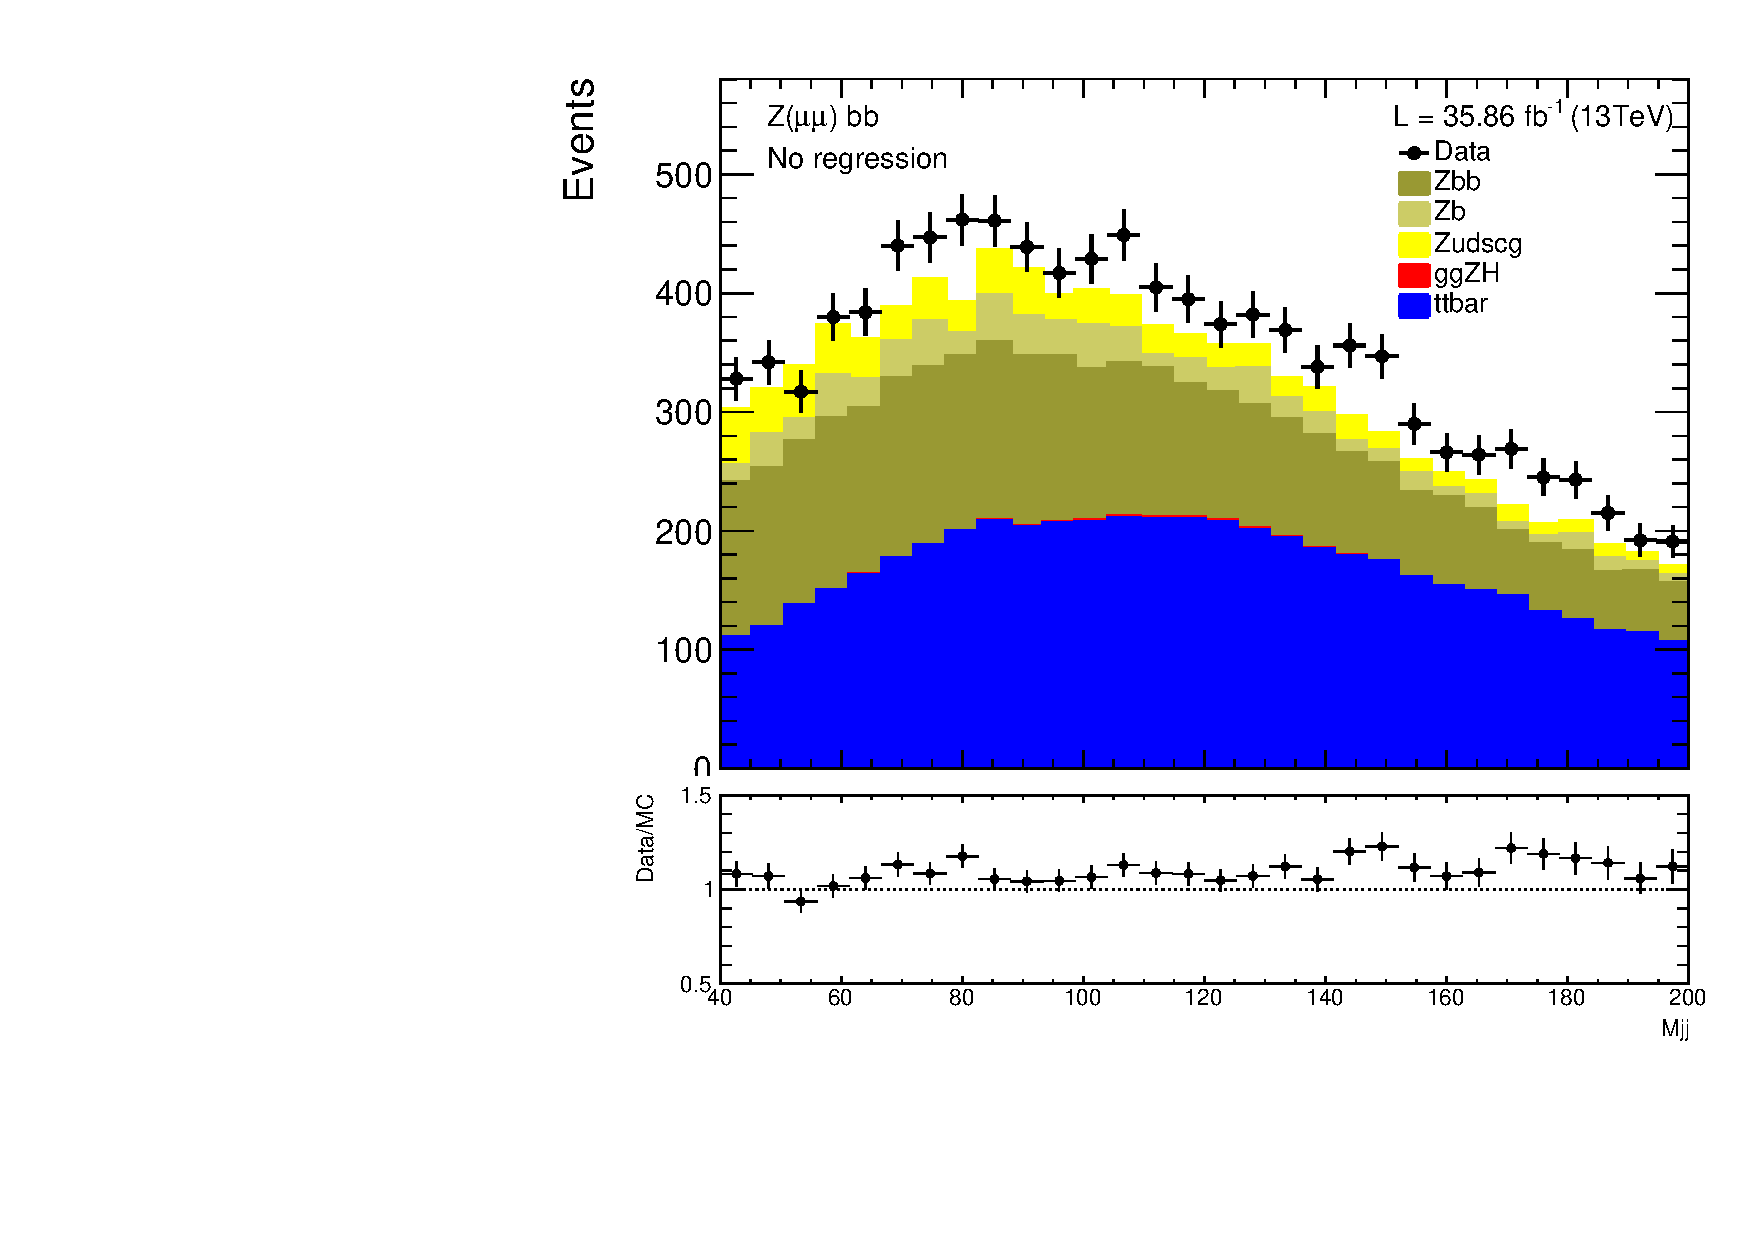
\includegraphics[width=0.32\textwidth]{b-reg/Vali_Data_MC_no_reg__Mjj_mu_Medium}\hfil
  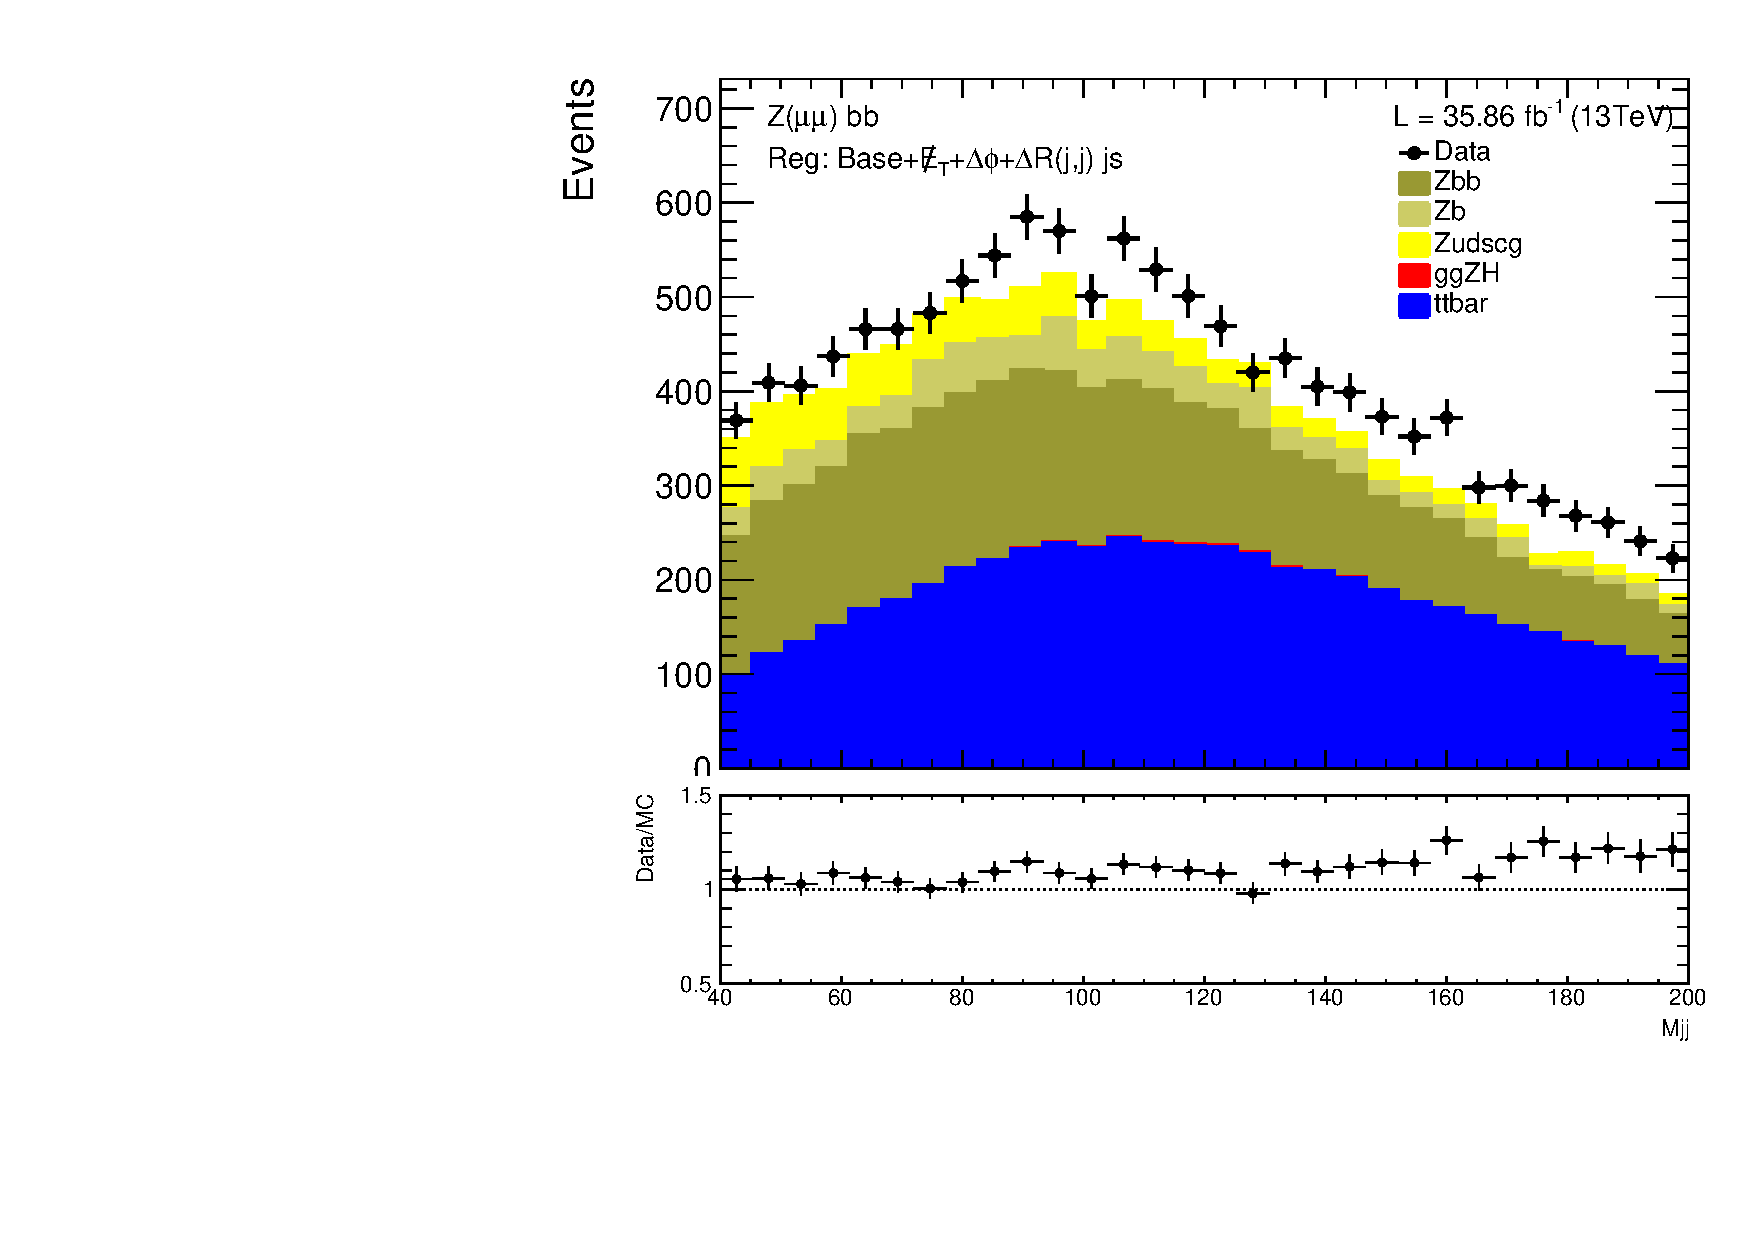
\includegraphics[width=0.32\textwidth]{b-reg/Vali_Data_MC_jet_15plus3_js_2_27__Mjj_mu_Medium}\hfil
  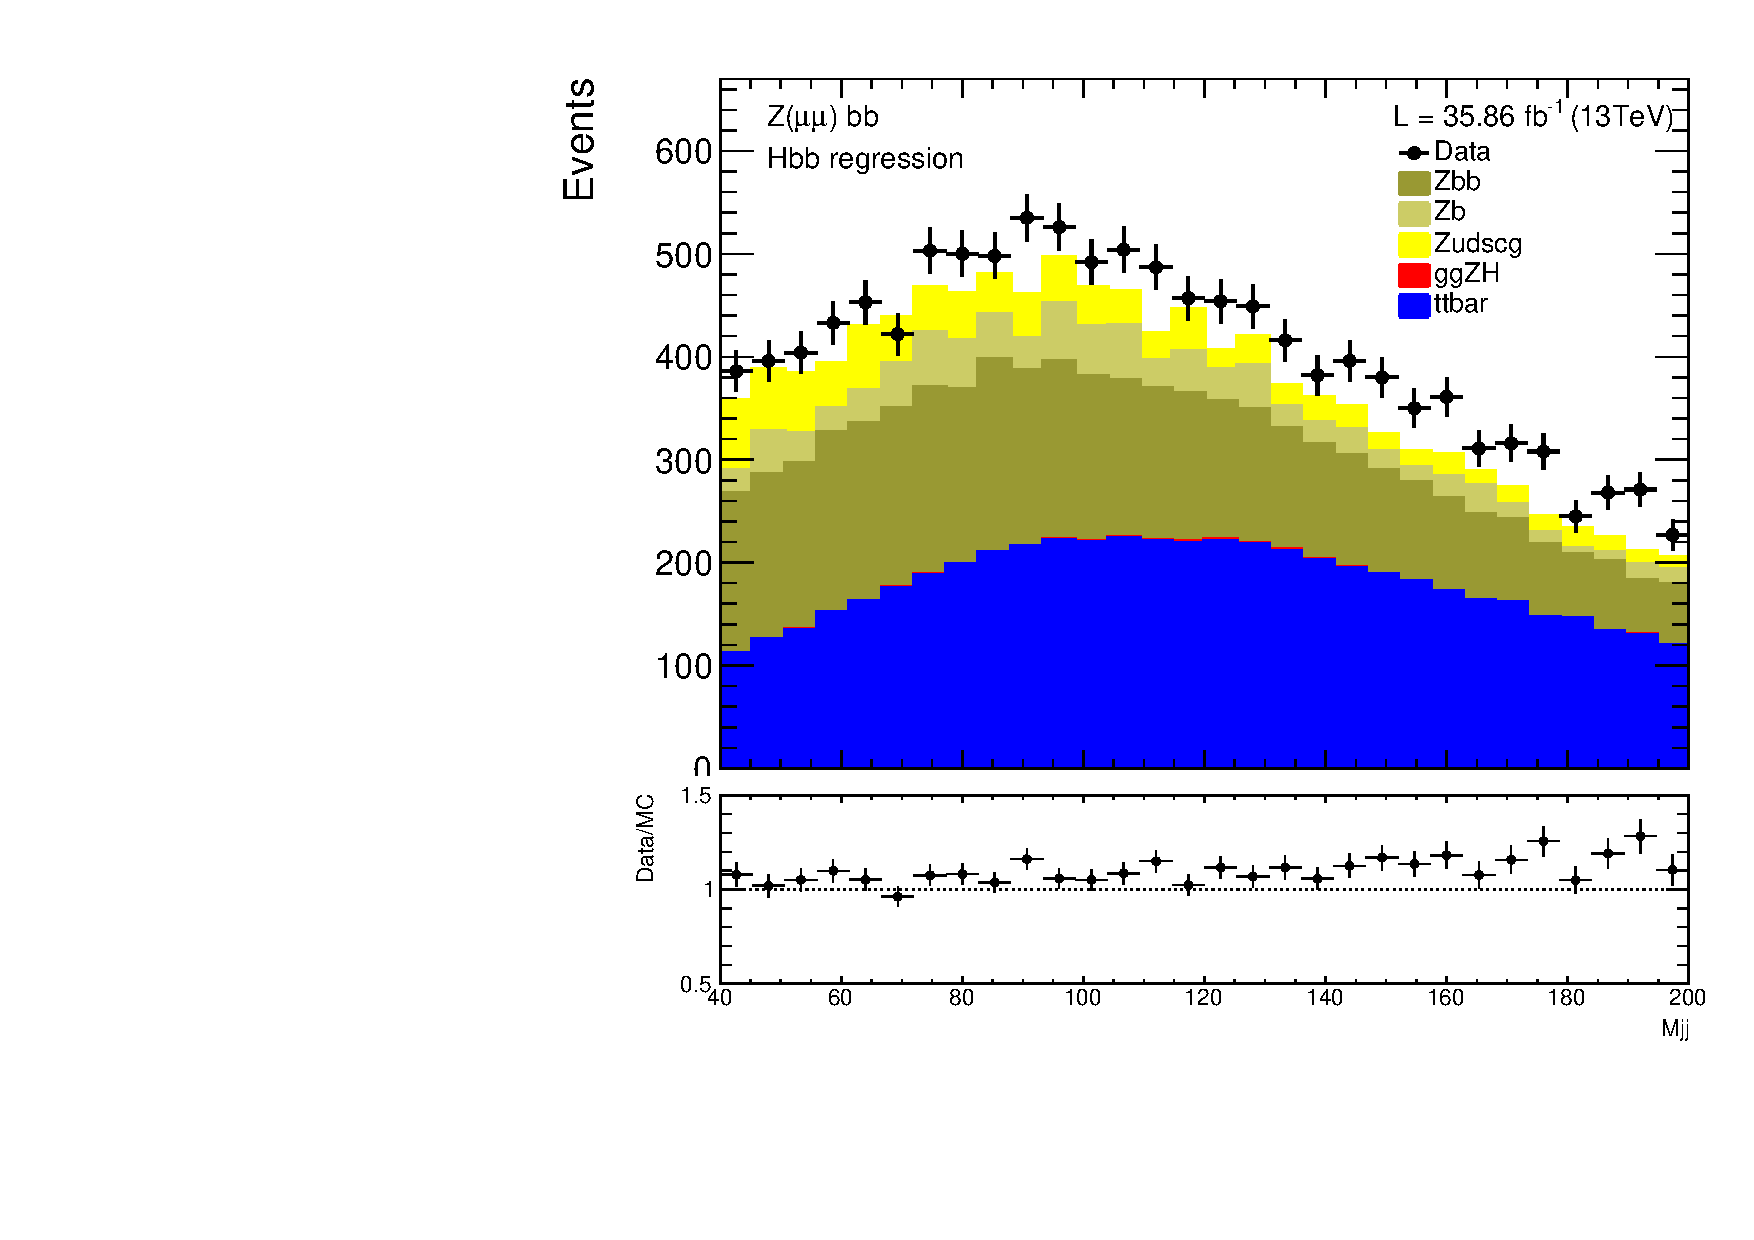
\includegraphics[width=0.32\textwidth]{b-reg/Vali_Data_MC_jet_Hbb__Mjj_mu_Medium}\hfil\\
  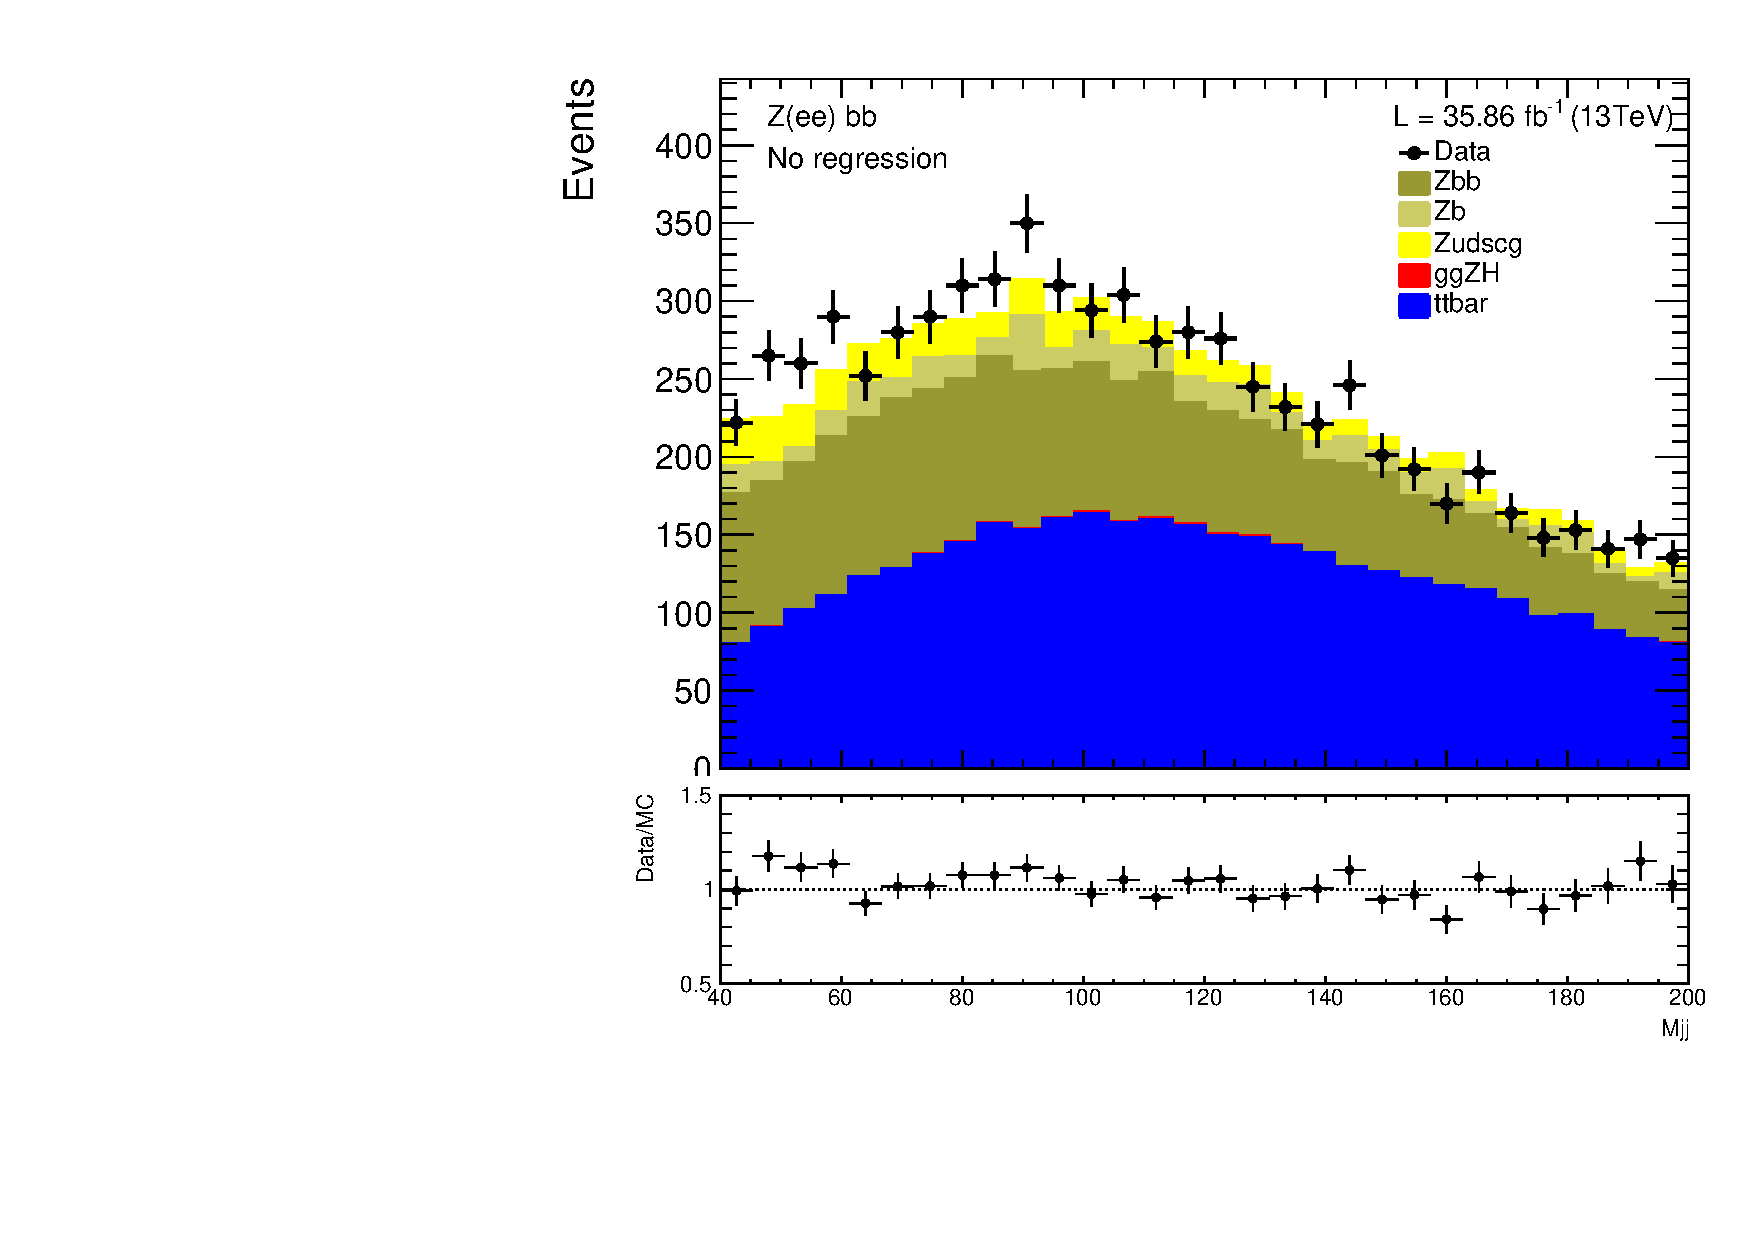
\includegraphics[width=0.32\textwidth]{b-reg/Vali_Data_MC_no_reg__Mjj_ele_Medium}\hfil
  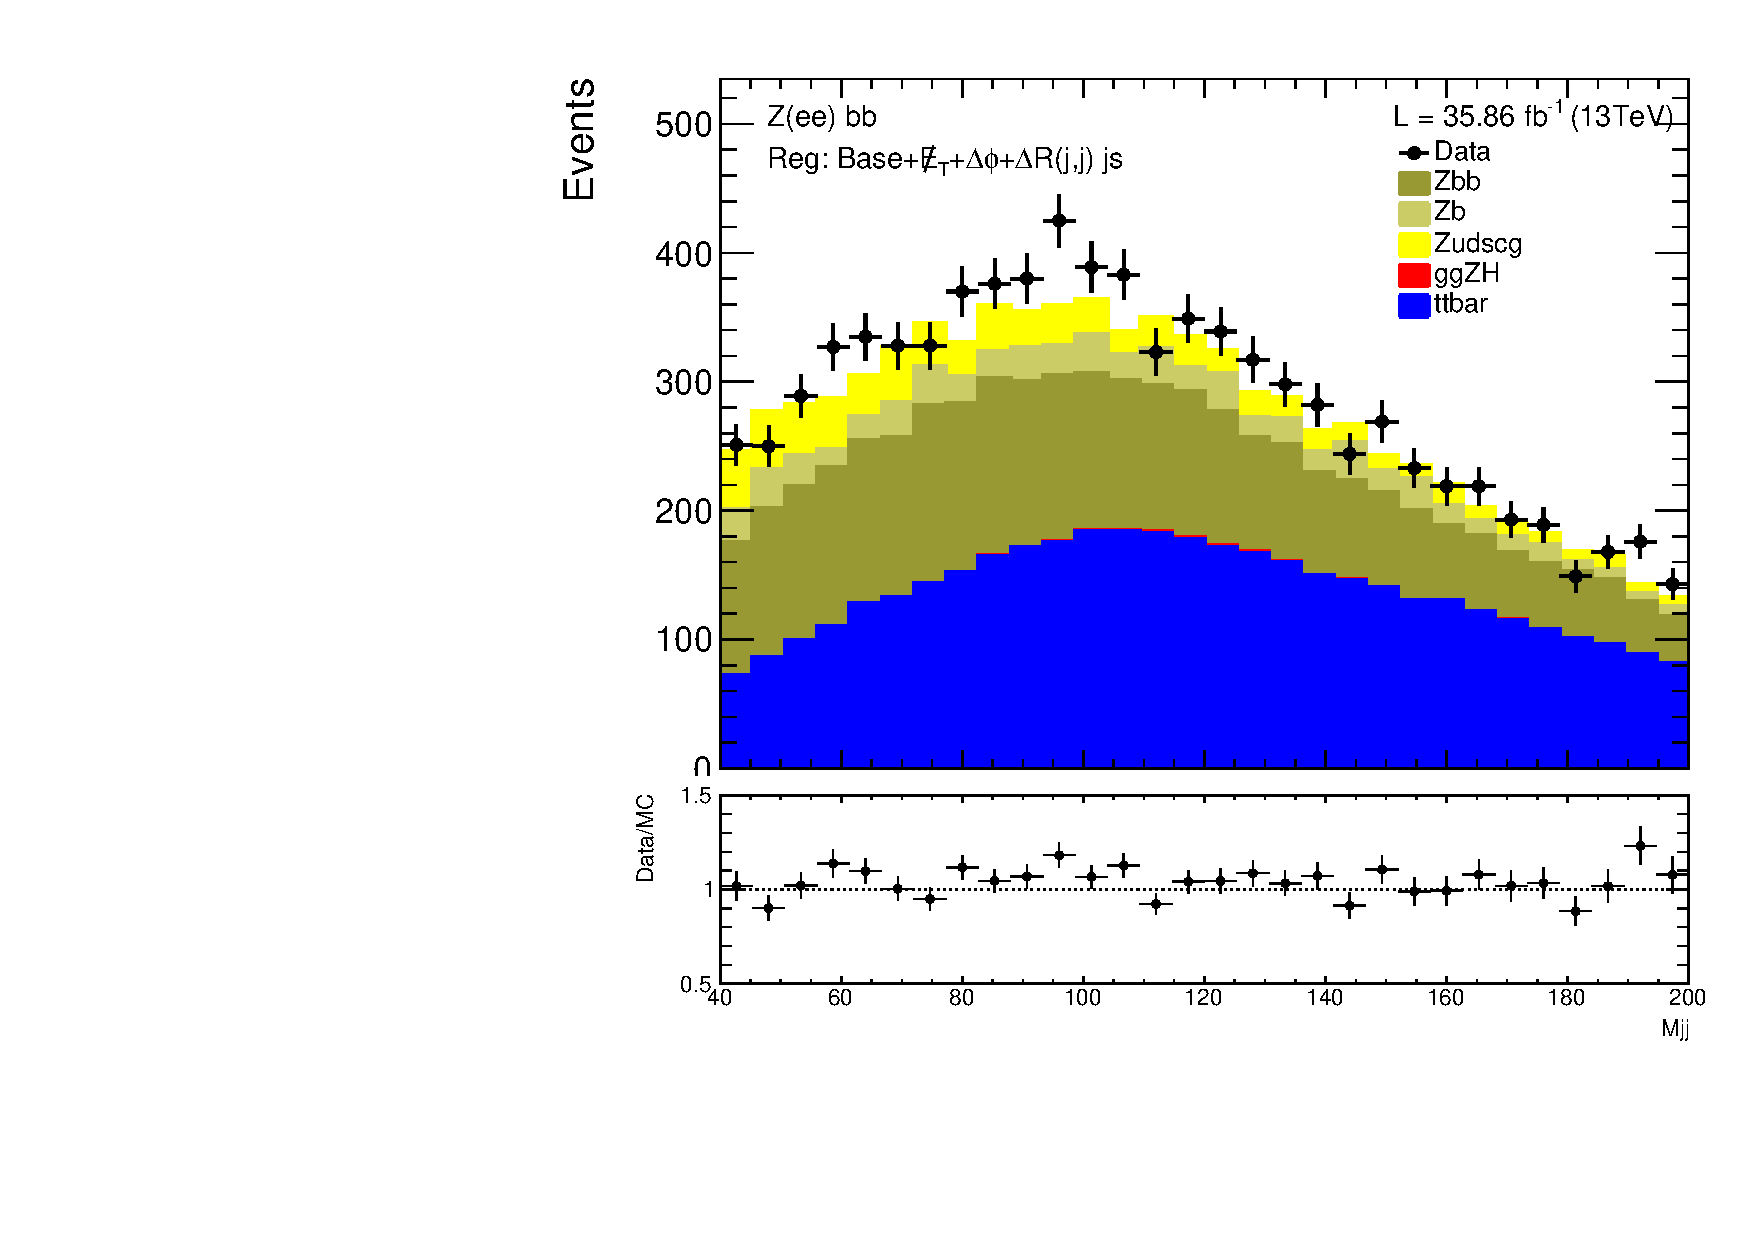
\includegraphics[width=0.32\textwidth]{b-reg/Vali_Data_MC_jet_15plus3_js_2_27__Mjj_ele_Medium}\hfil
  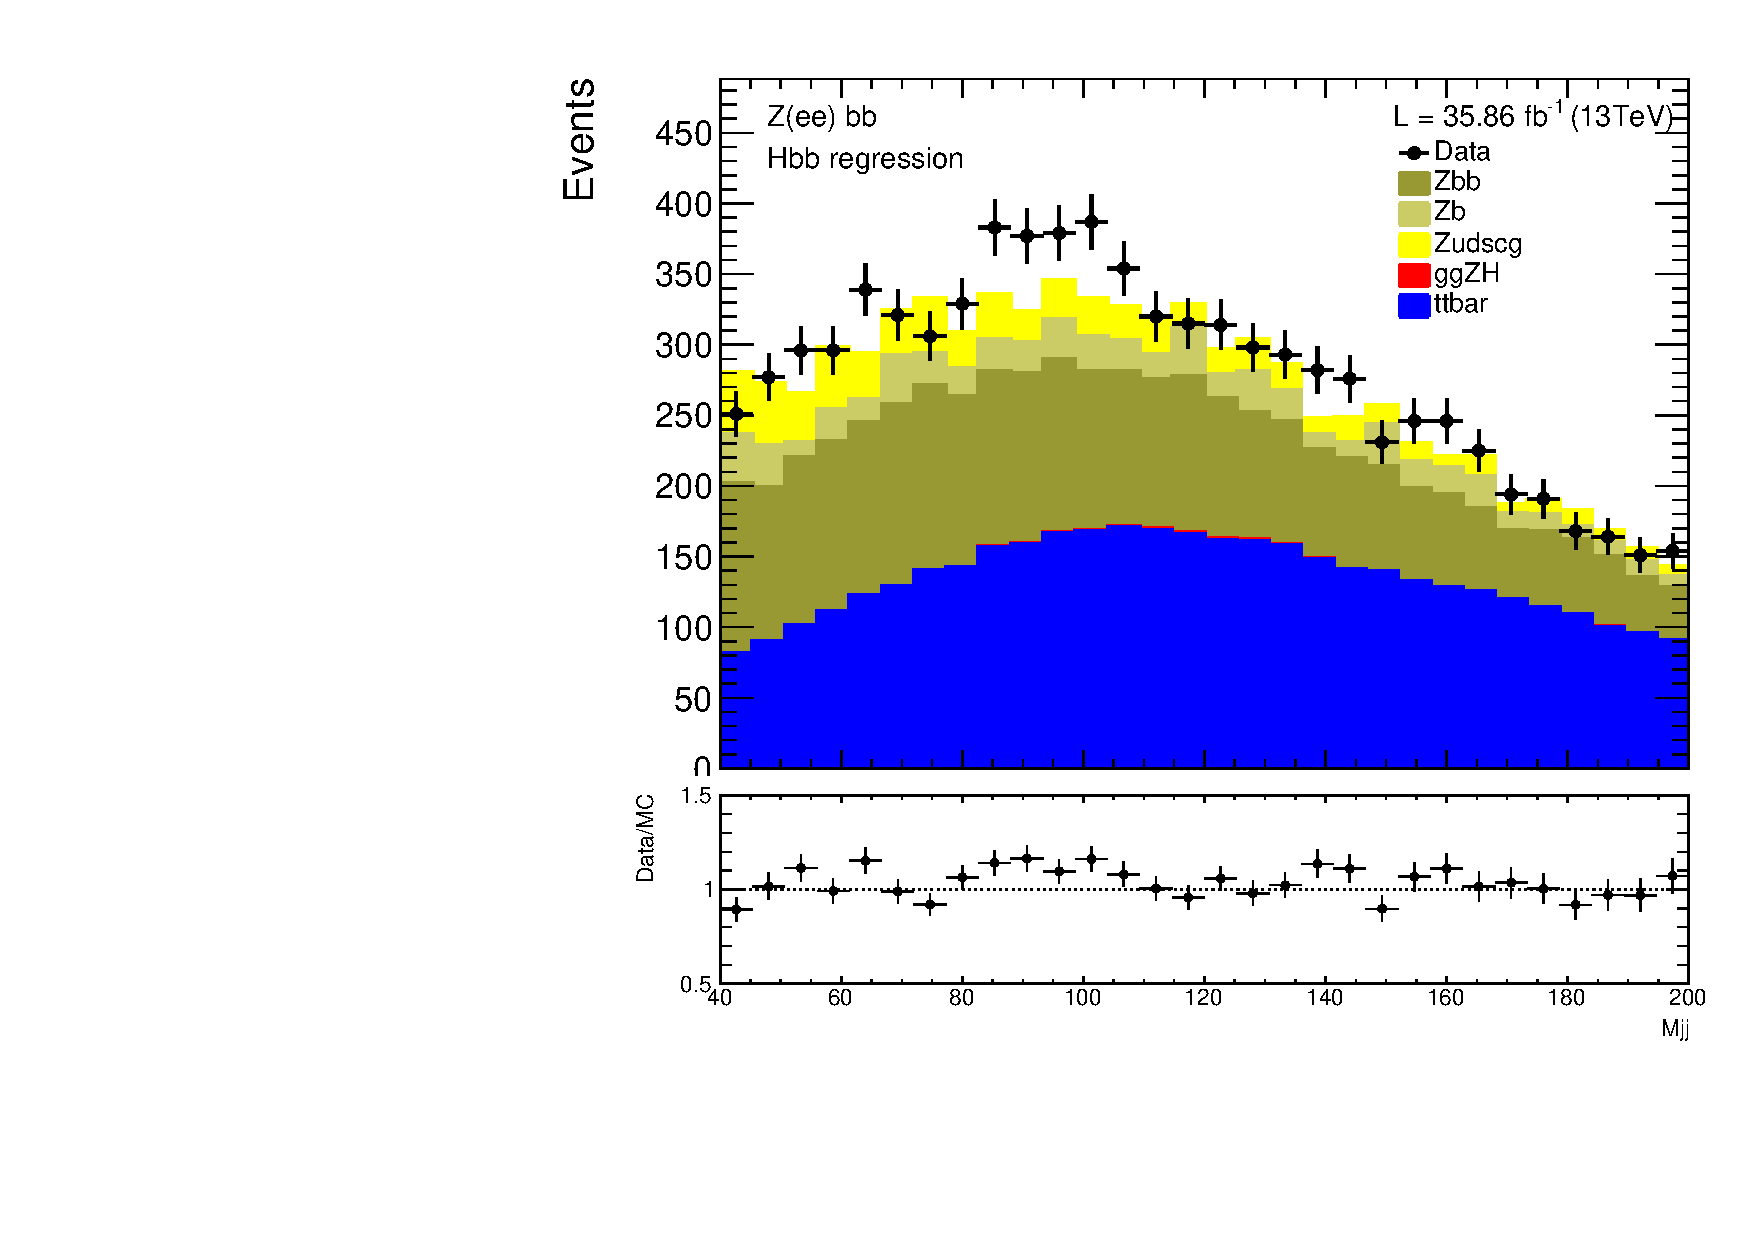
\includegraphics[width=0.32\textwidth]{b-reg/Vali_Data_MC_jet_Hbb__Mjj_ele_Medium}\hfil\\
  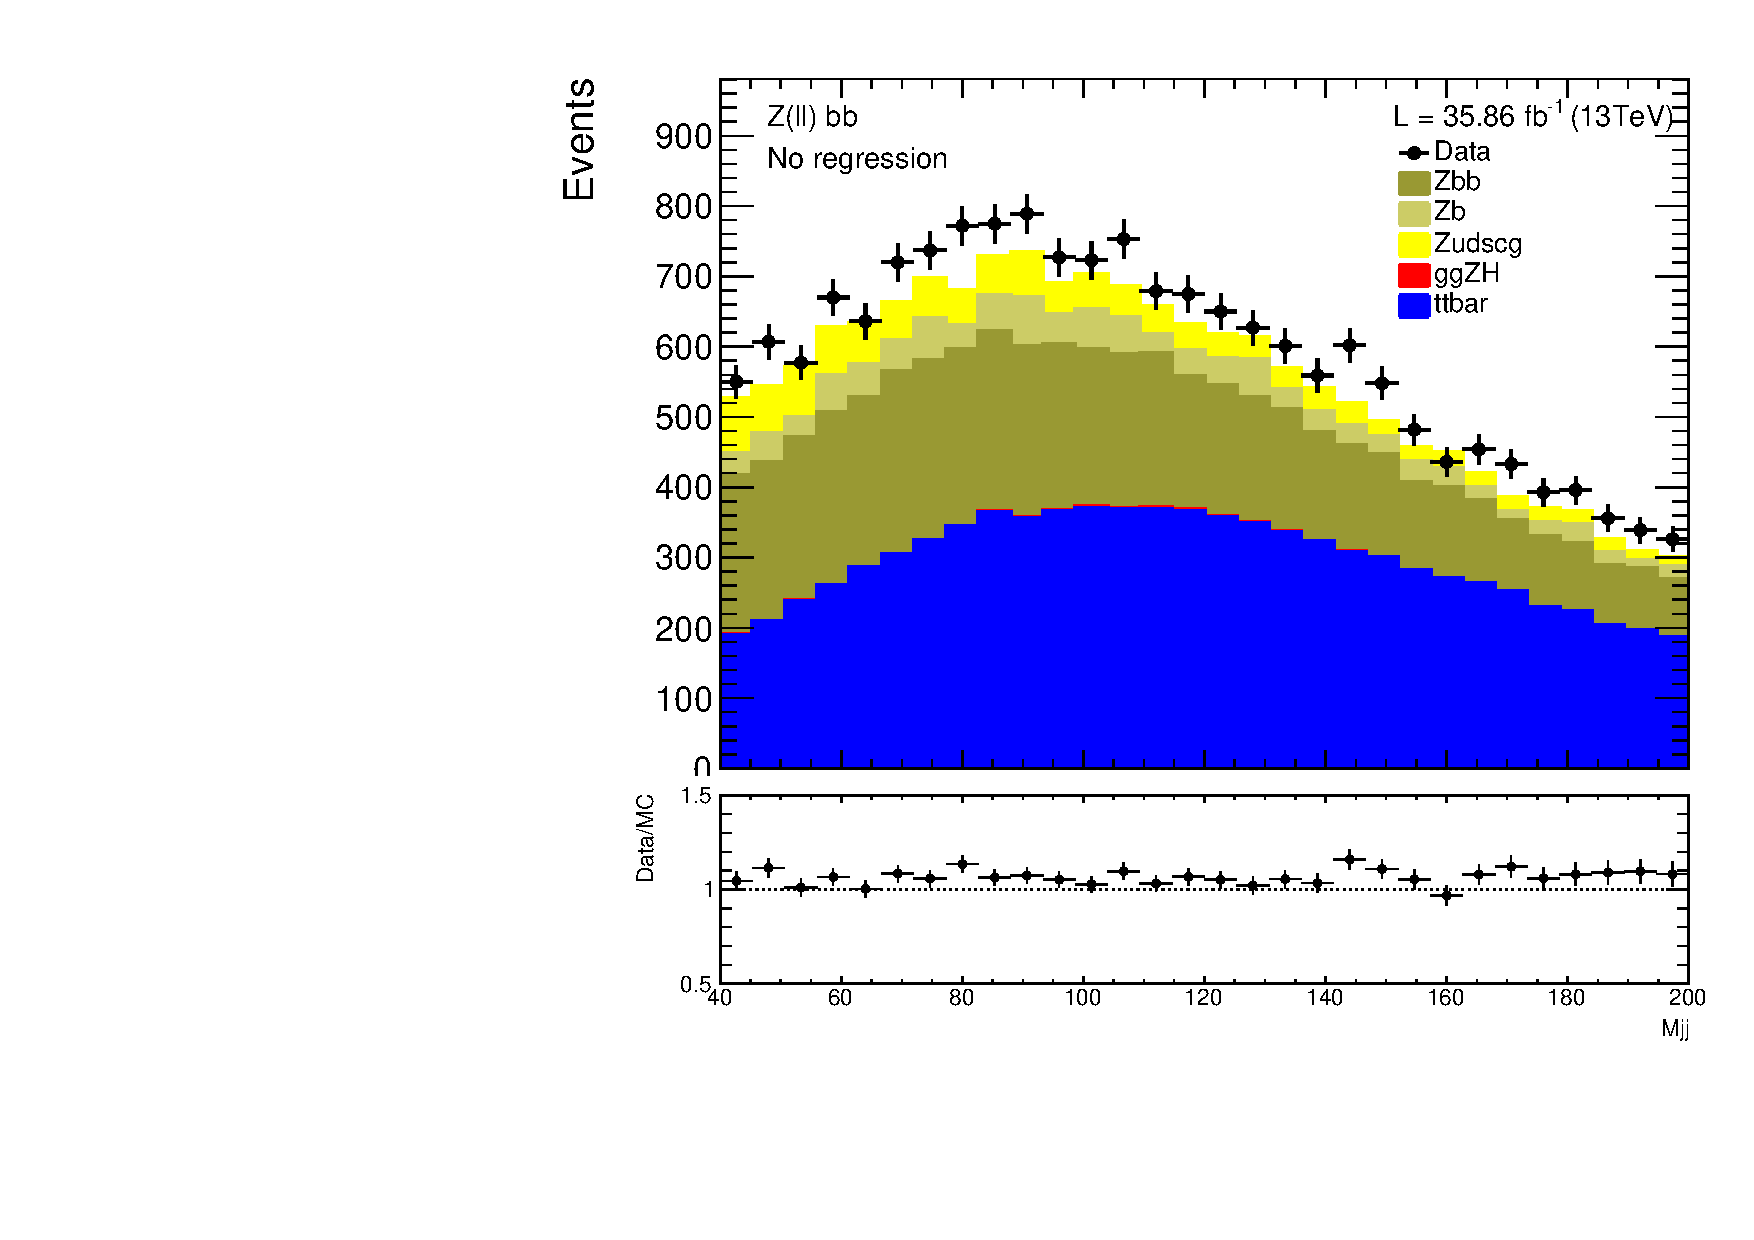
\includegraphics[width=0.32\textwidth]{b-reg/Vali_Data_MC_no_reg__Mjj_all_Medium}\hfil
  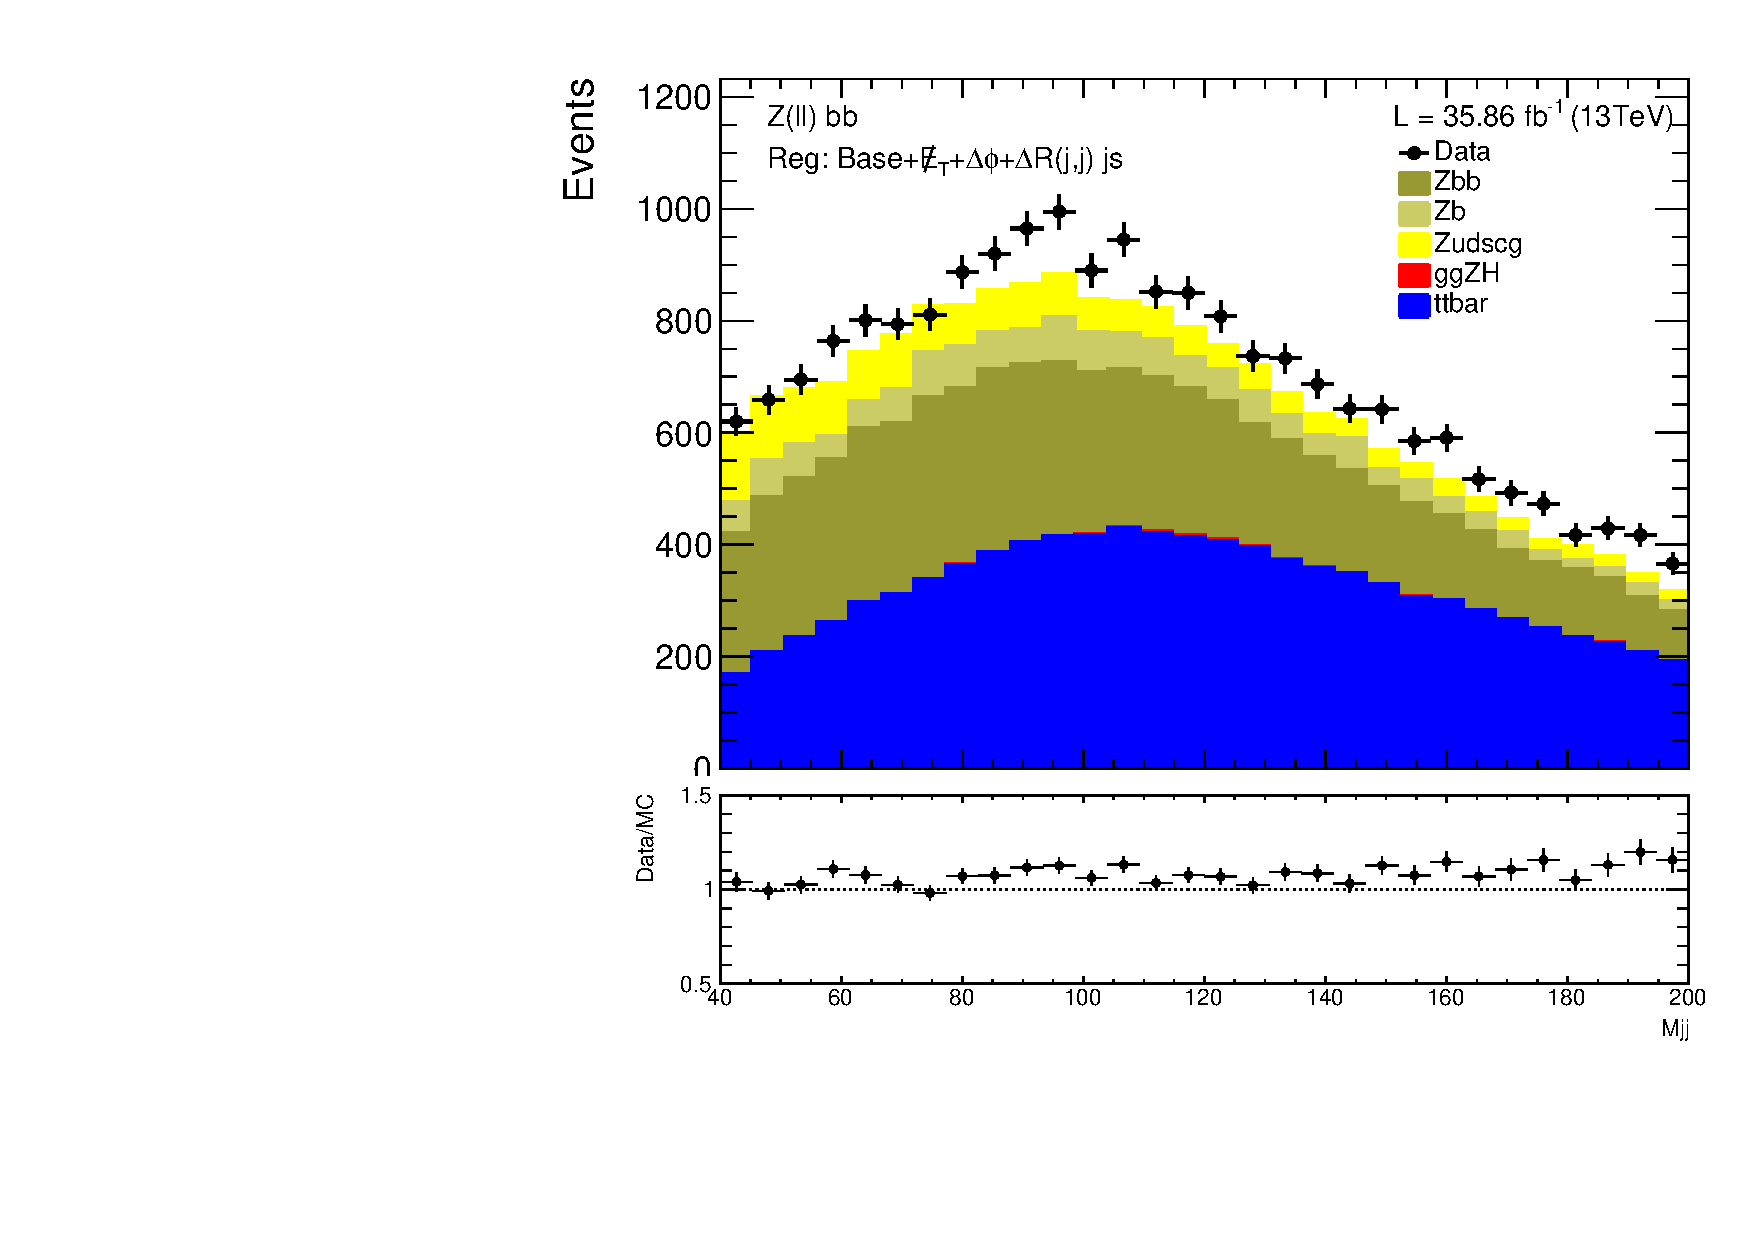
\includegraphics[width=0.32\textwidth]{b-reg/Vali_Data_MC_jet_15plus3_js_2_27__Mjj_all_Medium}\hfil
  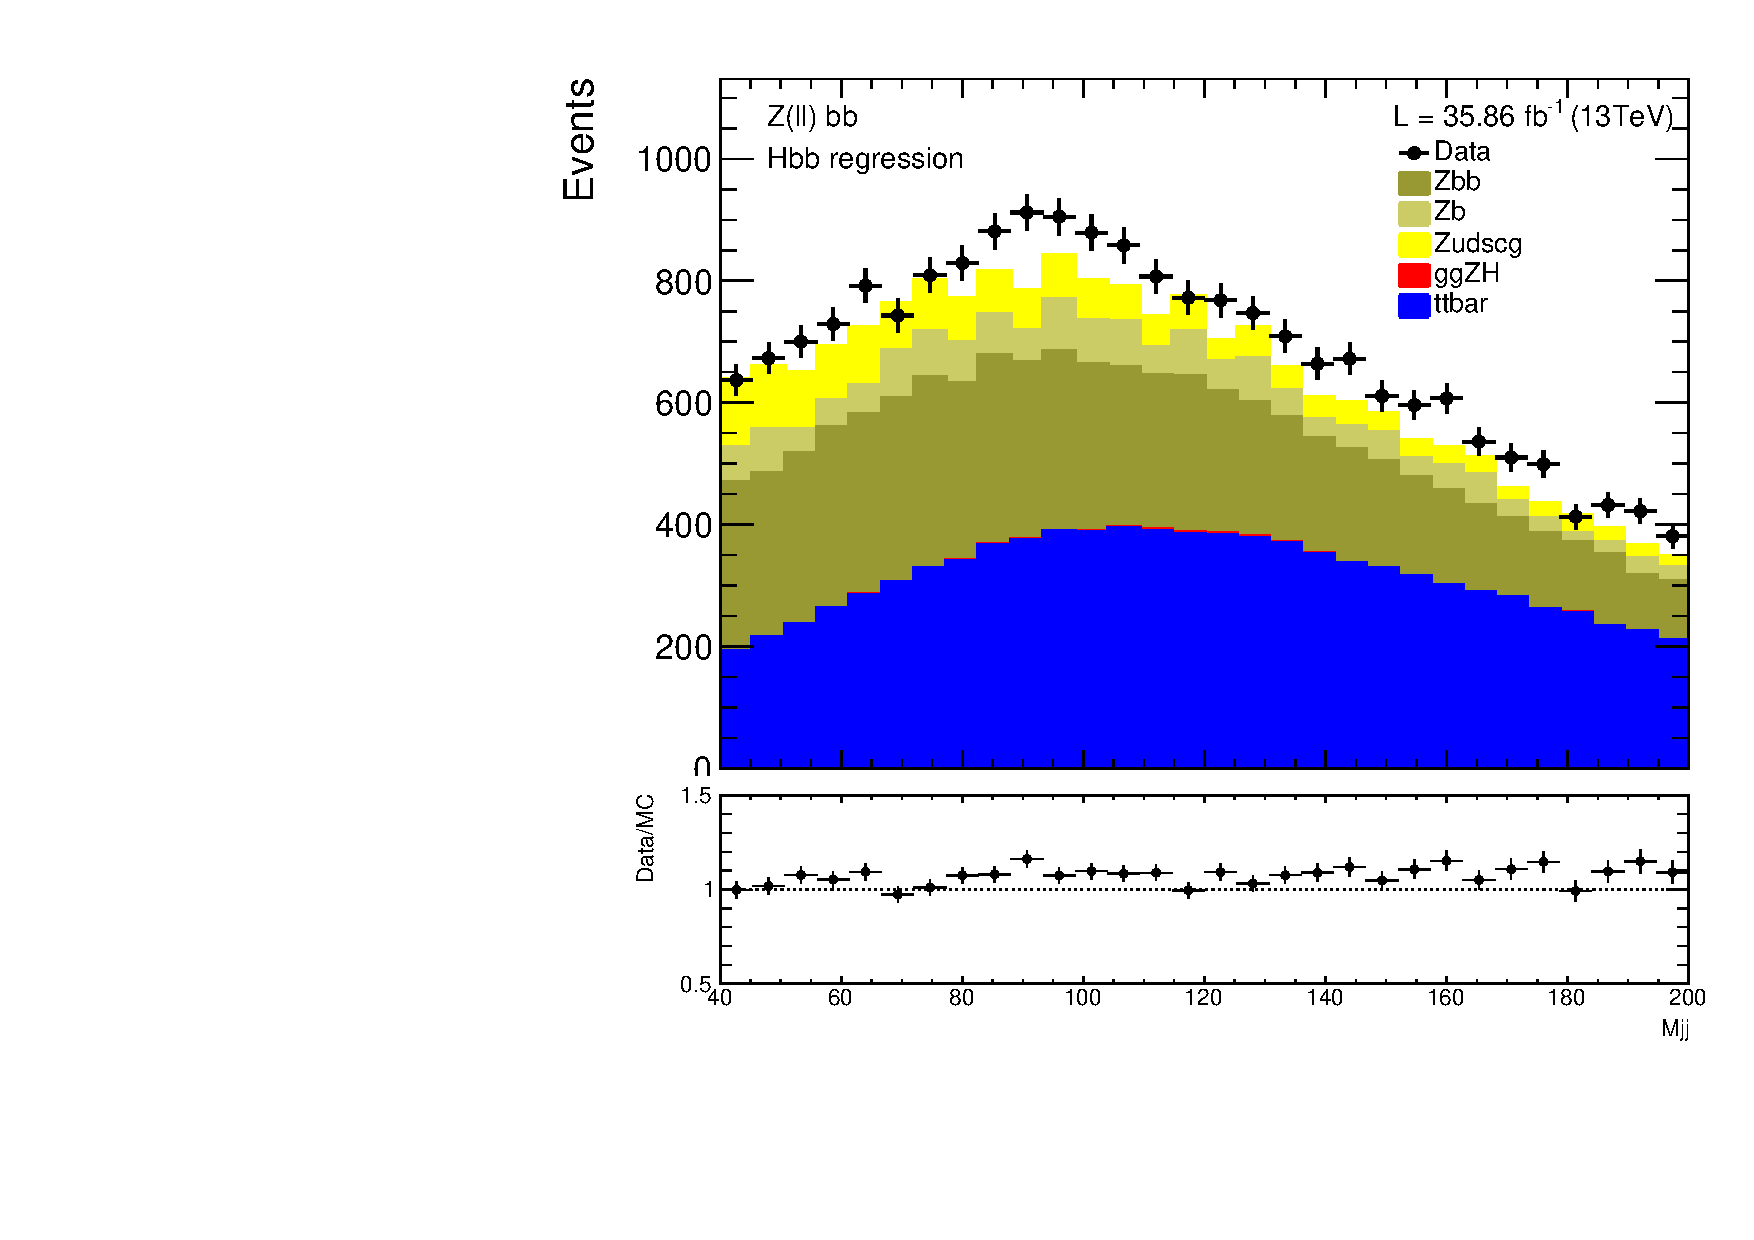
\includegraphics[width=0.32\textwidth]{b-reg/Vali_Data_MC_jet_Hbb__Mjj_all_Medium}\hfil\\
  \caption{Distributions of the $m_{jj}$. On the left are plots with
    no regression, in the center - using \textbf{full 15+3var js}
    training and on the right - using \textbf{Hbb} regression.  Top
    plots for muon channel, middle for electron channel and bottom is
    the combination (sum) of the two.  }
  \label{fig:vali-Mjj}
\end{figure*}

\clearpage

\subsubsection{B-tagging}
\label{sec:btag}

We utilize the \textit{Combined Secondary Vertex} algorithm (CSVv2) for tagging b-jets,
described in Ref.~\cite{btag-twiki}. This b-tagging score for leading and subleading jets is then used in the MVA categorization.

The b-tagging scale factors have been calculated according to the BTV recipe, including the in situ calculation of signal efficiency.
The signal efficiency has been calculated for all signal samples combined, in bins of $p_{T}$ and $|\eta|$.
The efficiency plots for tight WP, medium WP and loose WP can be seen in figure \ref{fig:btageff}.

\begin{figure*}[h]
  \centering
  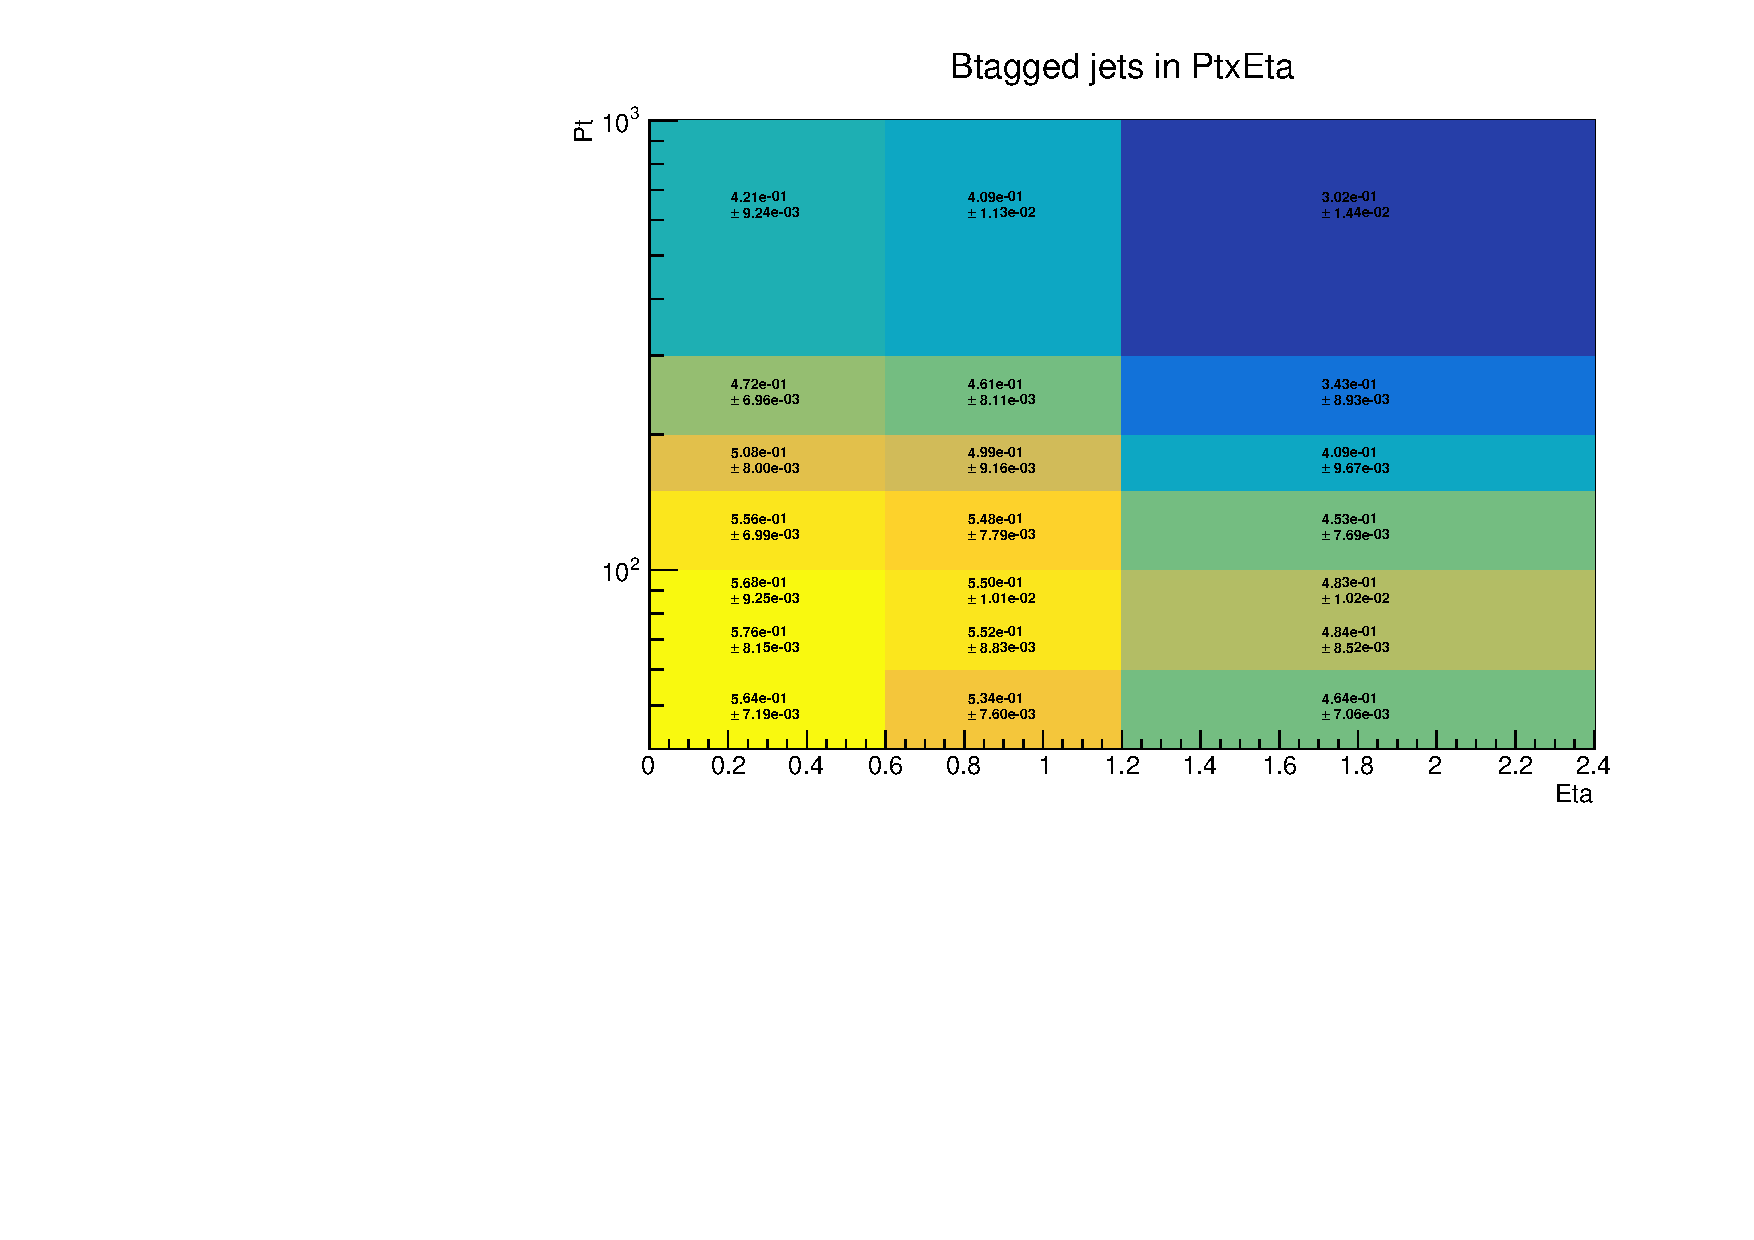
\includegraphics[width=0.45\textwidth]{figures/sec-jets/btageff_tight.pdf}\hfil
  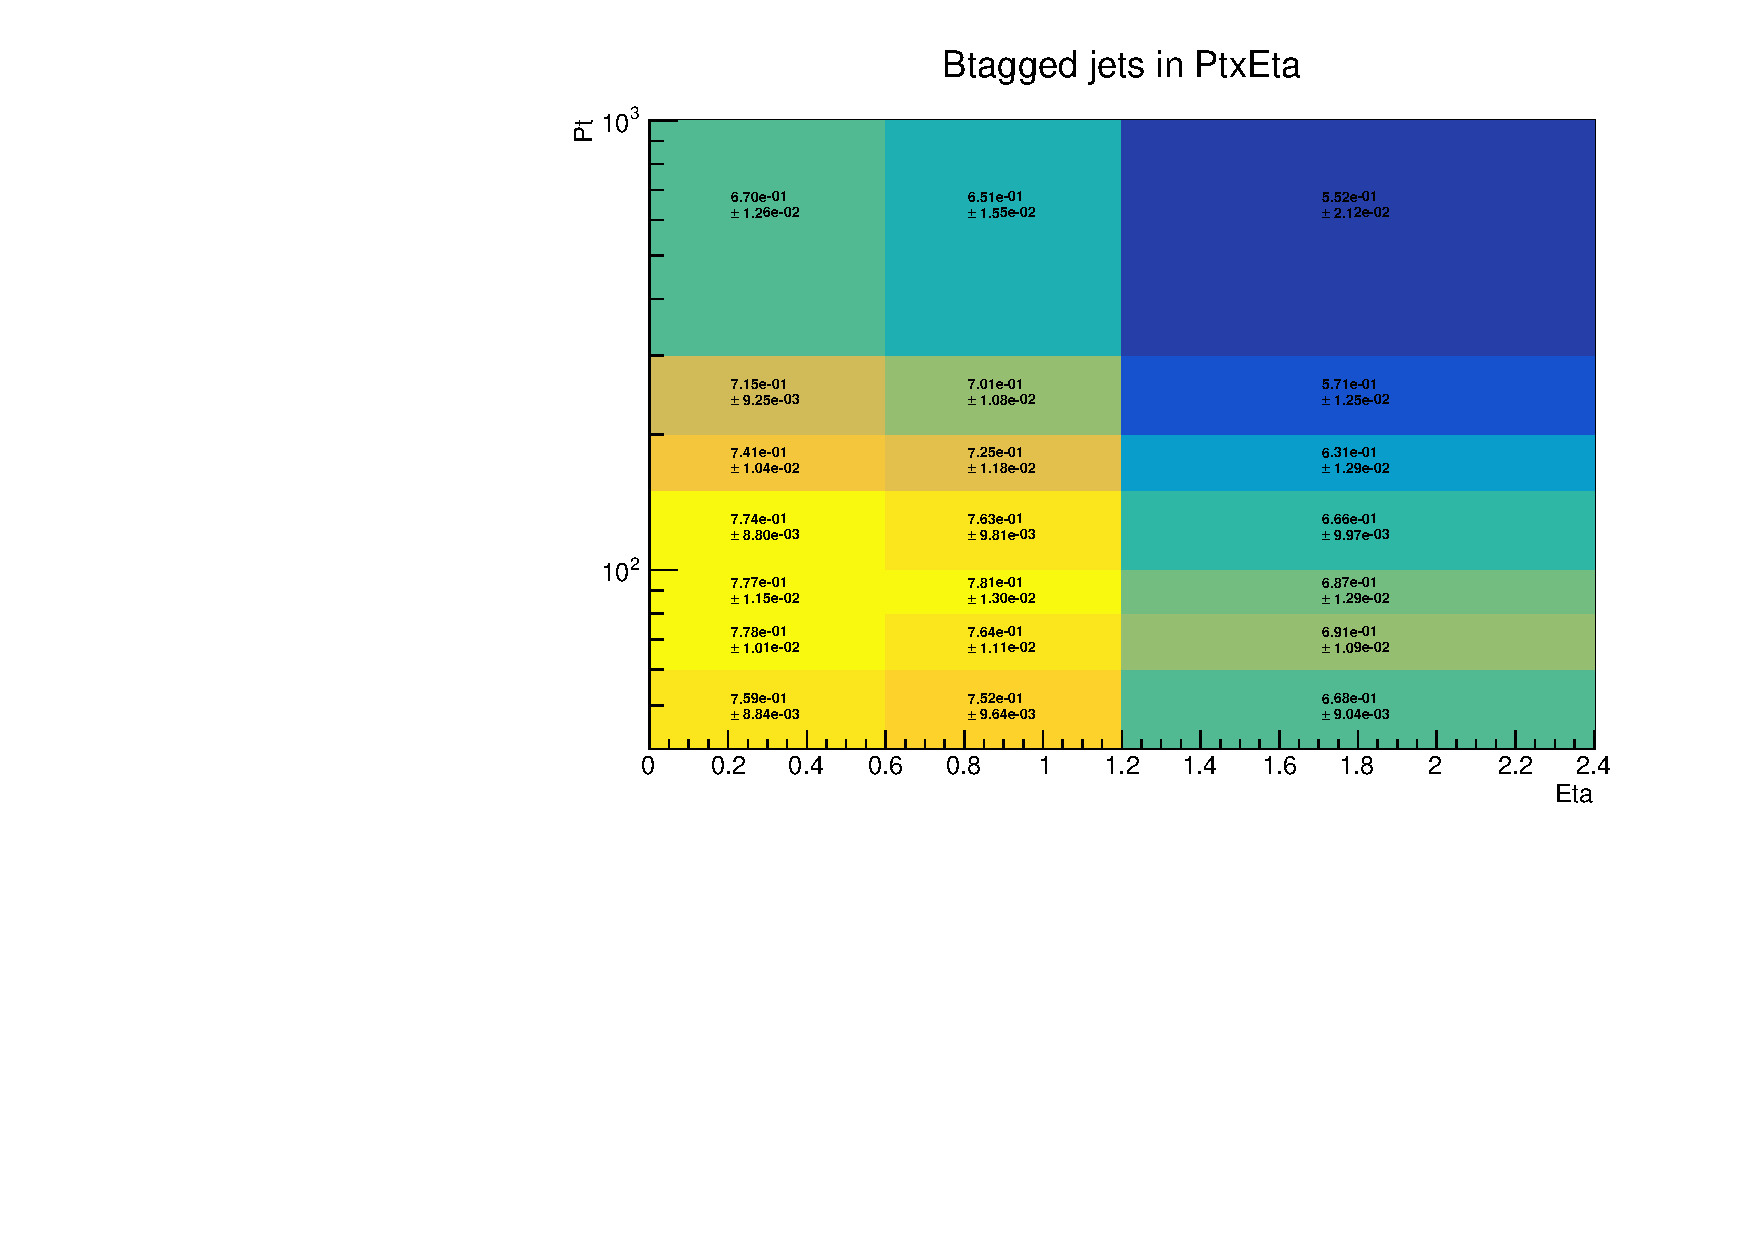
\includegraphics[width=0.45\textwidth]{figures/sec-jets/btageff_medium.pdf}\hfil
  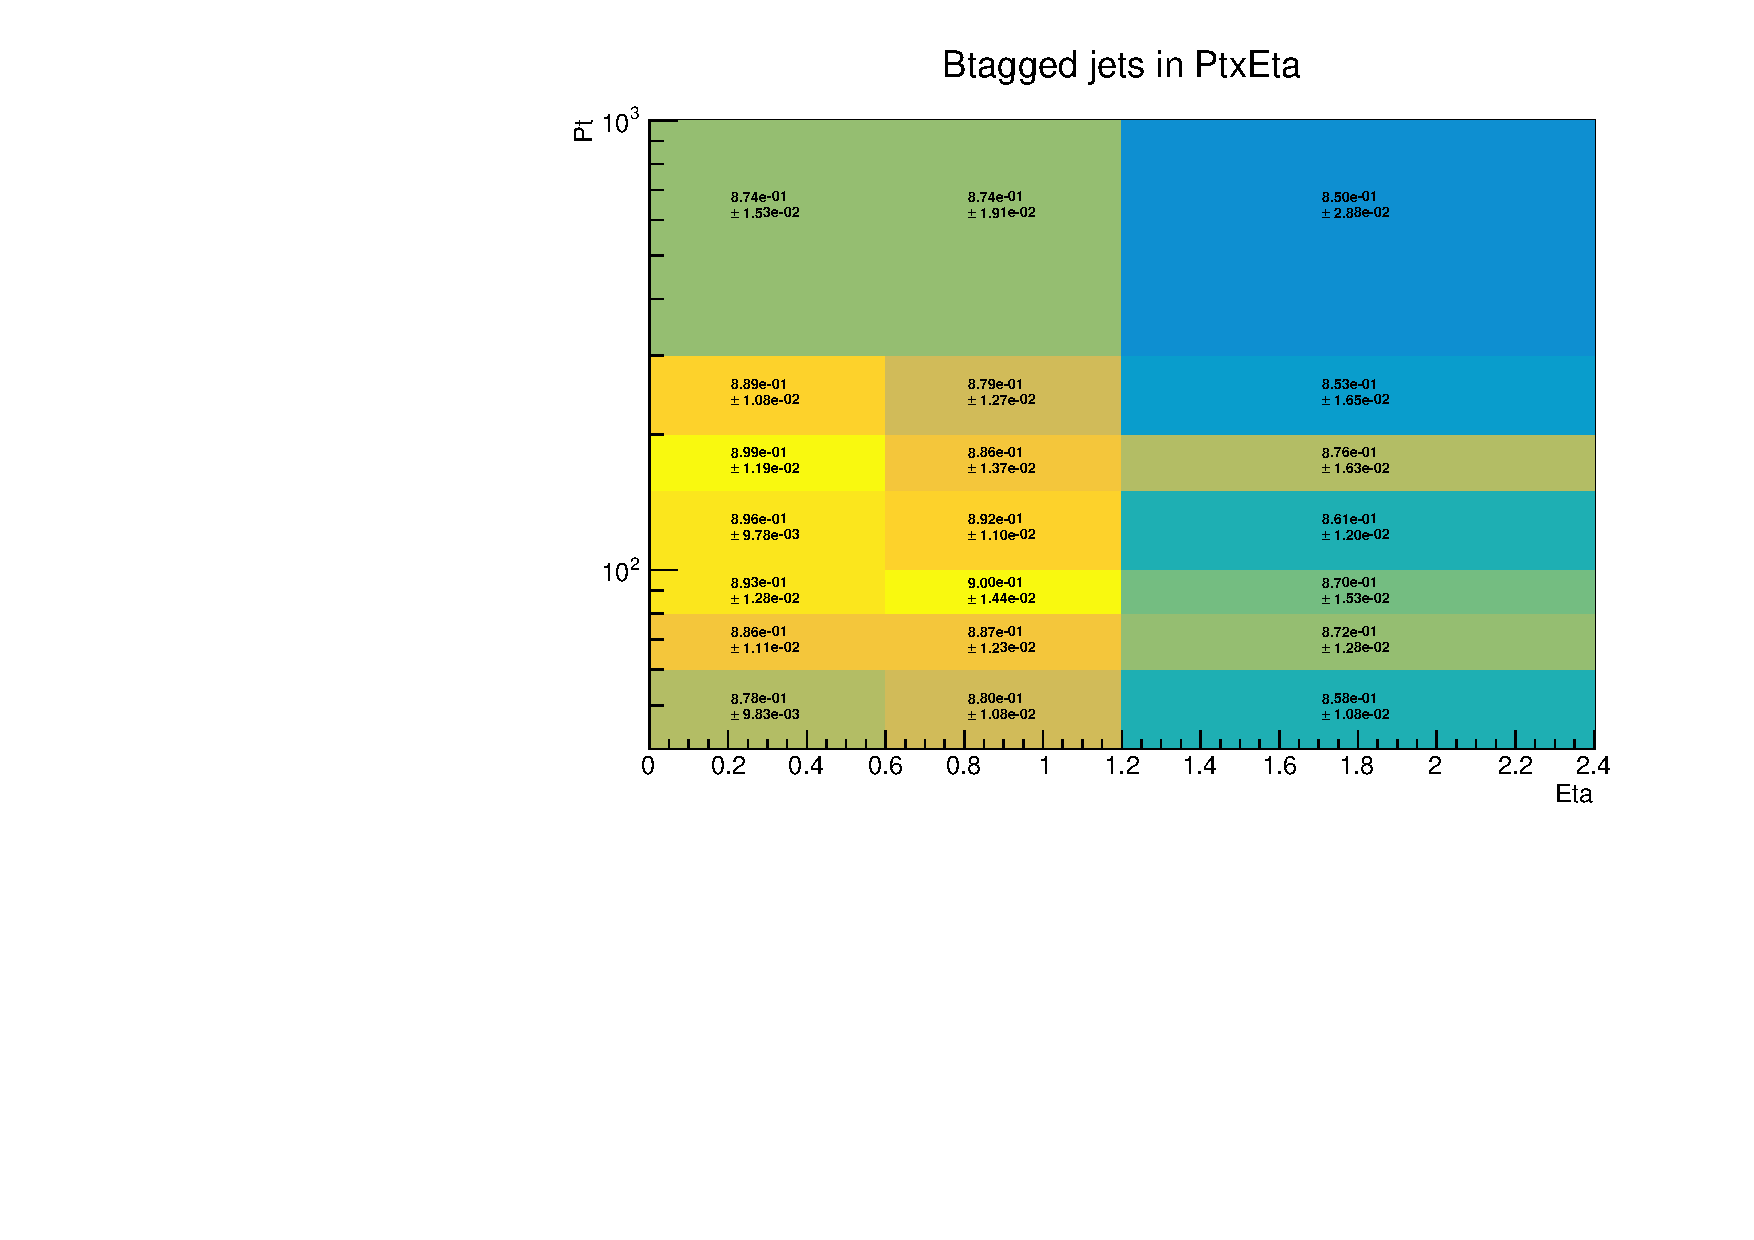
\includegraphics[width=0.45\textwidth]{figures/sec-jets/btageff_loose.pdf}\hfil 
  \caption{B-tagging efficiency for tight, medium and loose working points, as a function of jet $p_{T}$ and $|\eta|$.}
  \label{fig:btageff}
\end{figure*}


\clearpage
\section{MVA Based Categorization}
\label{sec:cats}

During the analysis, it has been noticed that different kinematic variables could potentially contribute to constraining the background contribution in the signal region without cutting too much on the signal efficiency. 
However, this large-dimensional optimization procedure (all investigated variables) was not optimal. 
Instead, we have developed a multivariate analysis (MVA), combining these different variables, into a single discriminant. 
This discriminant is used to categorize the events in High Purity, Medium Purity categories and a control region, similarly to the cut based categorization. 

The input variables investigated for this MVA were:
\begin{itemize}
\item Leading and subleading jets b-tagging score;
\item Helicity angles $|cos(\theta^{*}_{CS})|$, $|cos(\theta^{*}_{bb})|$ and $|cos(\theta^{*}_{\gamma\gamma})|$: $|cos(\theta^{*}_{CS})|$ is defined as the angle between the direction of the $H\rightarrow\gamma\gamma$ candidate to the Colin-Sopper reference frame (assumes each incoming particle in the scattering to have 6.5 TeV); $|cos(\theta^{*}_{xx})|$ is defined as the angle between the particle $x$ and the direction defined by the $H\rightarrow x x$ candidate (randomly choosing between x's), where $x = \gamma$ or $b$;
\item $p_{T}(\gamma\gamma)/M(jj\gamma\gamma)$ and $p_{T}(jj)/M(jj\gamma\gamma)$
\end{itemize}

The training was performed in the photon control region, as described in \ref{sec:PCR}. 
Plots comparing the input variables in the photon control region and the blinded signal region are shown in Figure \ref{fig:inputmva}. 
As our signal in the training, we sum the 14 non-resonant HH samples available (box only, SM, and 12 BSM points). 
Thus, we have a training that is not specific to a single region in the parameter space, maintaining the sensitivities comparable between the benchmark points (as it is with the cut based categorization). 

\begin{figure*}[h]
  \centering
  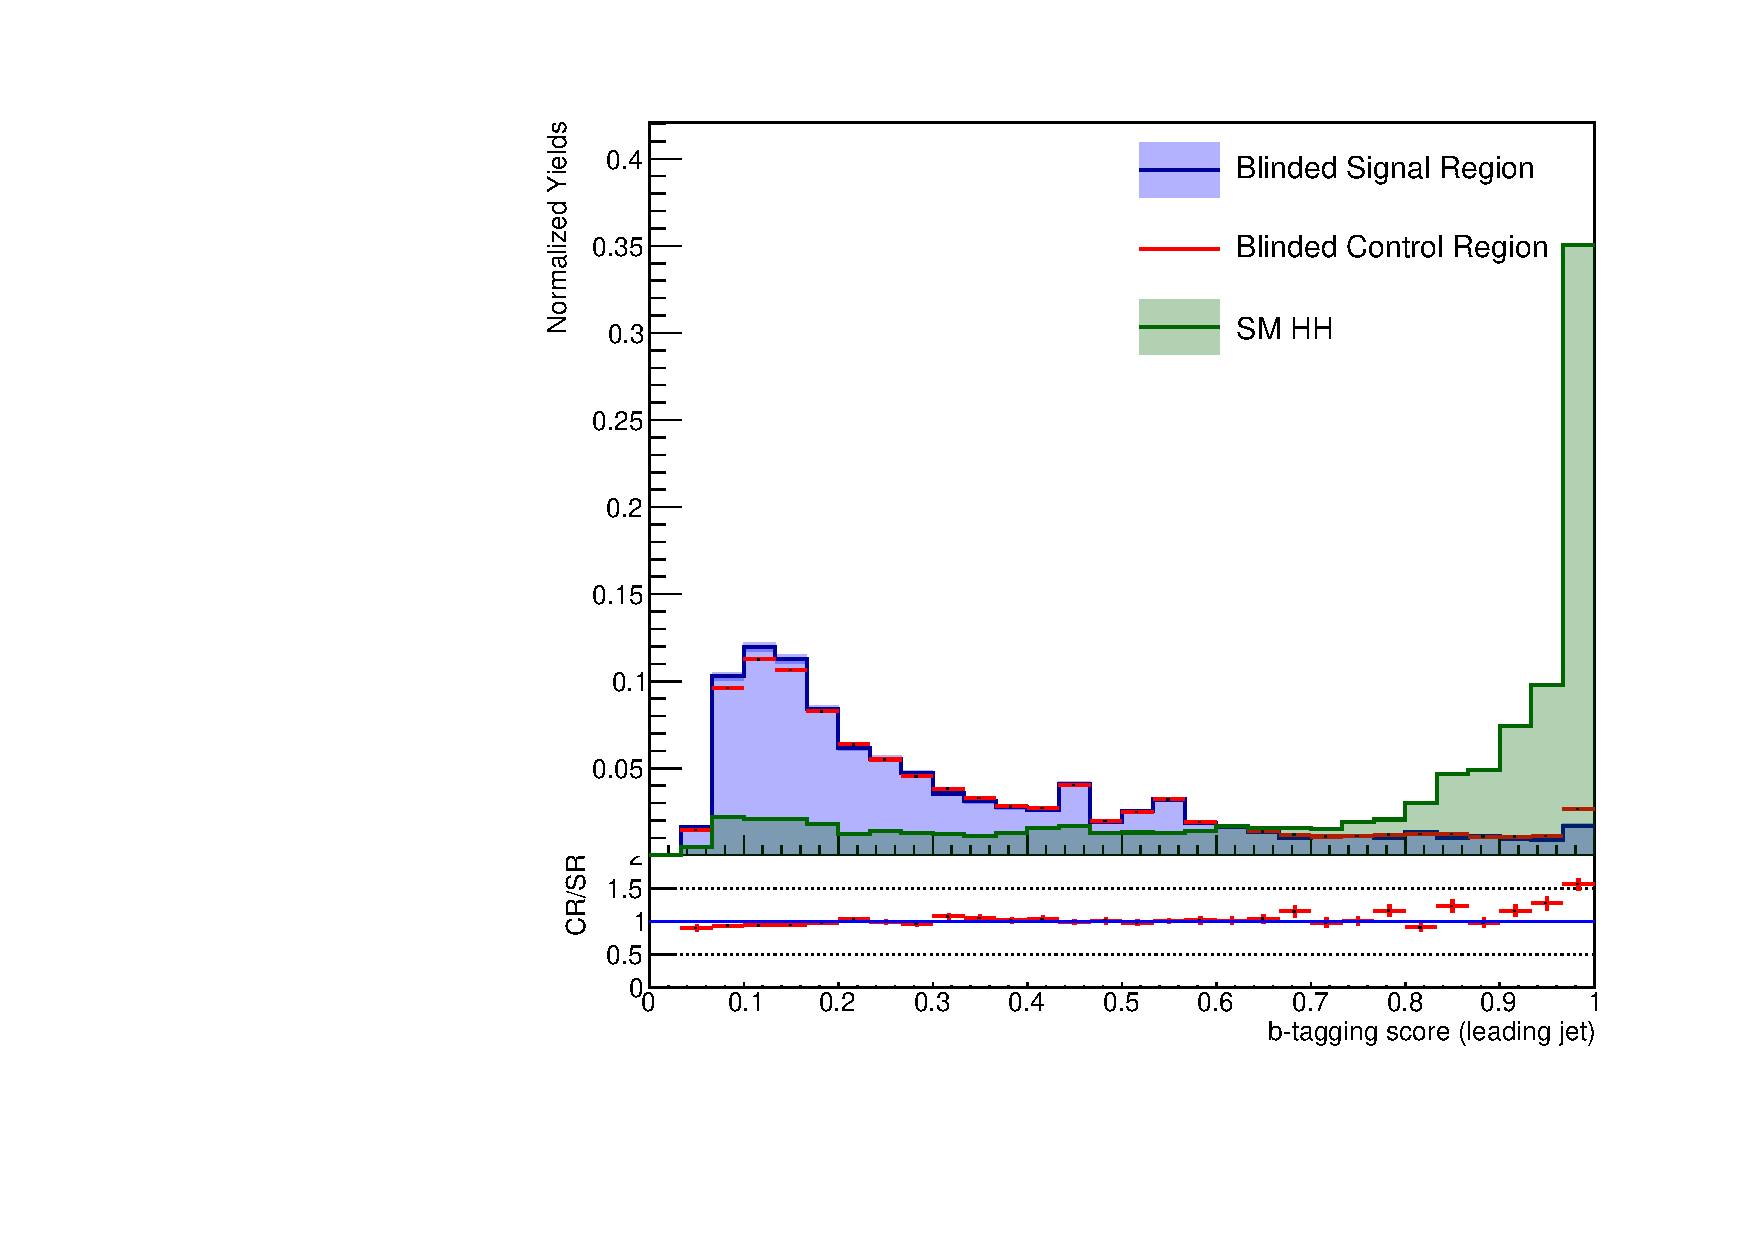
\includegraphics[width=0.3\textwidth]{figures/sec-cats/mva/ljbdis}\hfil
  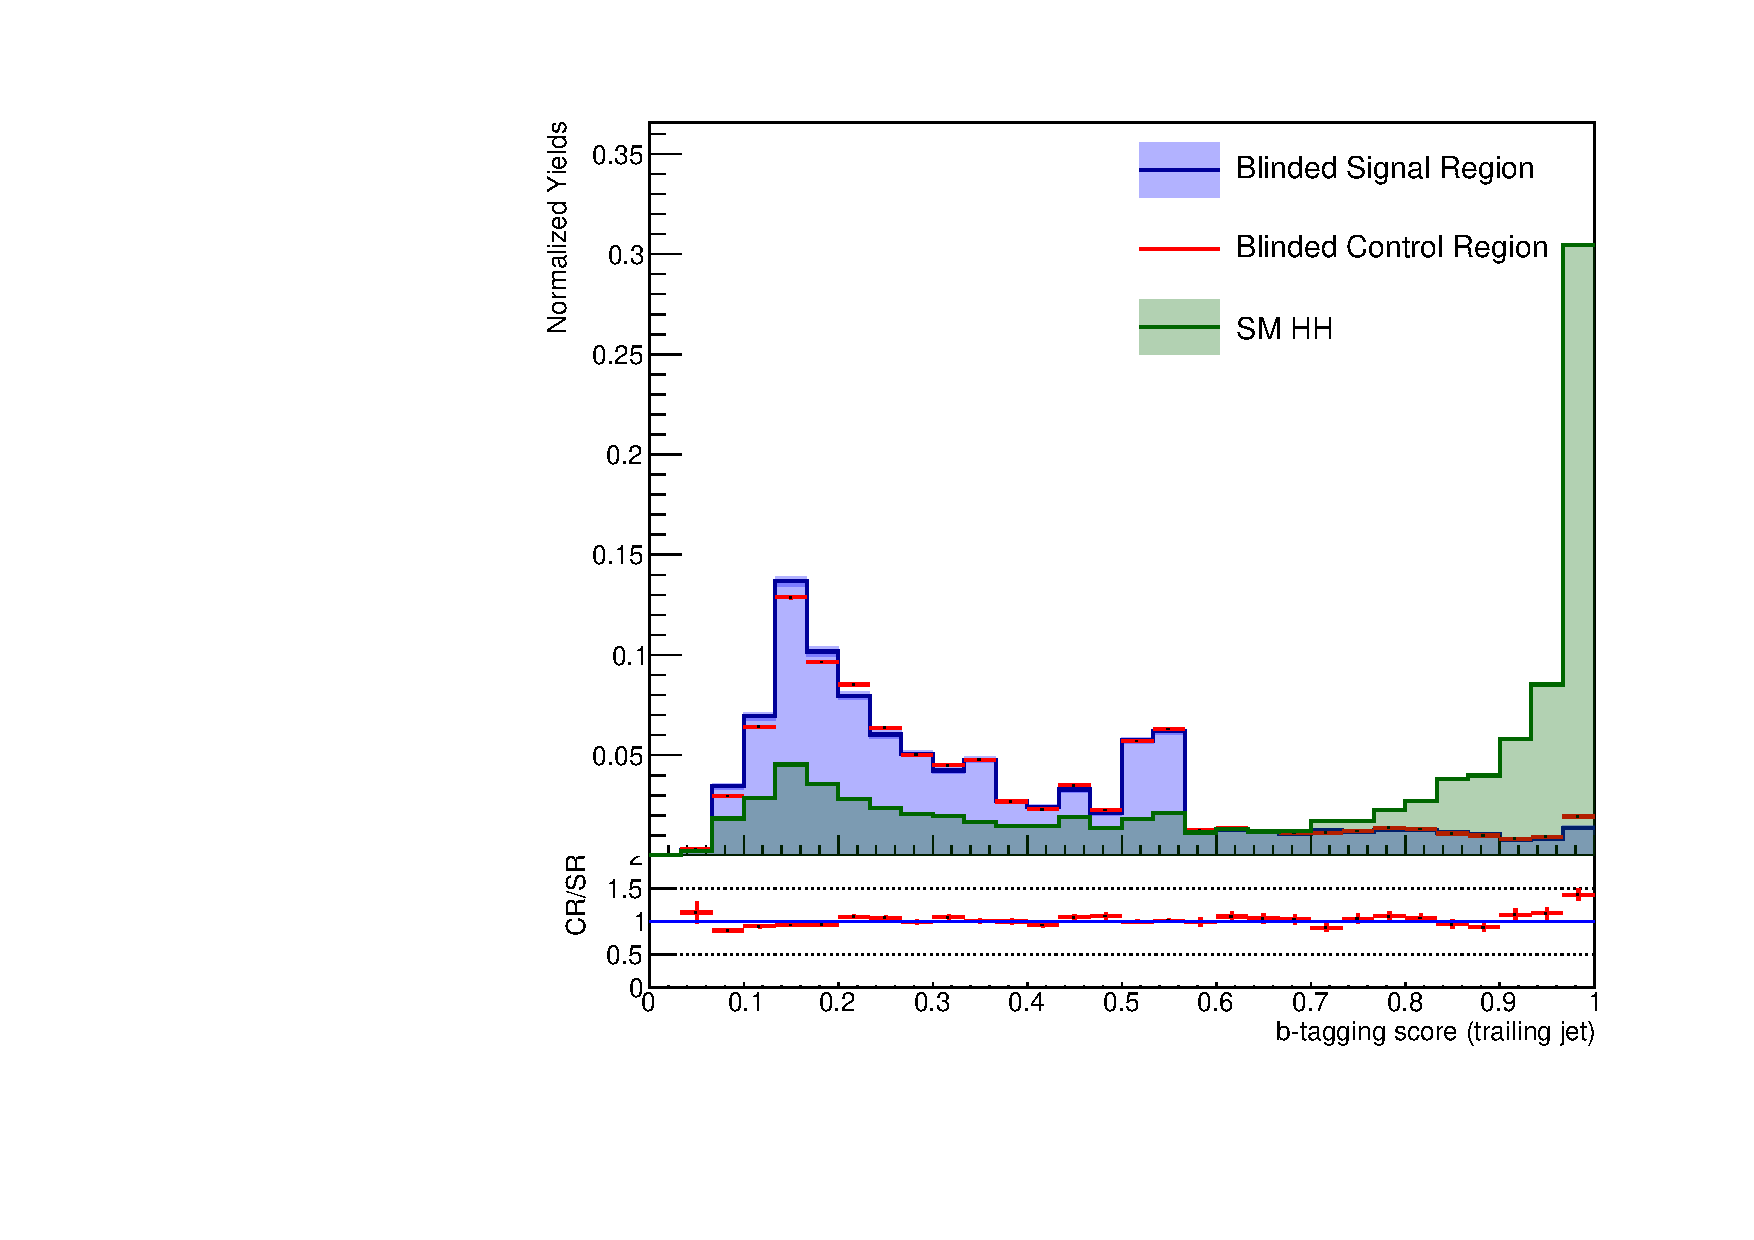
\includegraphics[width=0.3\textwidth]{figures/sec-cats/mva/sjbdis}\hfil
  \includegraphics[width=0.3\textwidth]{figures/sec-cats/mva/cts_cs}\hfil
  \includegraphics[width=0.3\textwidth]{figures/sec-cats/mva/ct_bb}\hfil
  \includegraphics[width=0.3\textwidth]{figures/sec-cats/mva/ct_gg}\hfil
  \includegraphics[width=0.3\textwidth]{figures/sec-cats/mva/gghhr}\hfil
  \includegraphics[width=0.3\textwidth]{figures/sec-cats/mva/bbhhr}\hfil
  \caption{Distributions of input variables in the blinded photon control region, blinded signal region, and SM HH sample. All normalized to unity. }
  \label{fig:inputmva}
\end{figure*}

To improve the training, we split the training into two regions: low mass and high mass. 
The low mass training is performed with events with $\tilde{M}_{X}$ below 350 GeV, while the high mass training uses the complementary region. 
The training is based on a decision tree boosted with the gradient algorithm, with the trees randomized between iterations to decrease overtraining. 
To implement the training the TMVA package was used. 
%The TMVA output plots are shown for both trainings in Figures \ref{fig:mva_hm} and \ref{fig:mva_lm}. 
From now on, we will refer to the training discriminant variable as HHTagger.

With the HHTagger discriminant, we build our two signal categories based on the optimization of the expected SM HH limit, separately in the high mass and in the low mass regions. 
These categories are called high purity category (HPC) and medium purity category (MPC); their names refer to their signal and background content. 
As signal, we use the SM HH sample to calculate the sensitivity. 
The outcome of this study was the categorization in Table \ref{tab:catmva}. 
The expected number of background events, when comparing MPC and HPC between cut based and MVA approaches, is comparable and consistent, while for the number of signal events, the performance is better for the HHTagger categorization. 

We also have to ensure that the HHTagger selection does not distort our variables of interest, $\Mjj$ and $\Mgg$. 
We demonstrate that there is no appreciable shaping by comparing the $\Mjj$ and $\Mgg$ shapes in different bins of the HHTagger discriminant. 
This can be seen in Figure \ref{fig:mva_mggmjj}. 

\begin{table}
\centering
    \begin{tabular}{| c | c | c |}
    \hline
    Mass Region & HPC & MPC \\ \hline
    Low Mass & HHTagger $> 0.96$ & $ 0.75 < $ HHTagger $ < 0.96 $ \\ \hline 
    High Mass & HHTagger $> 0.96$ & $ 0.6 < $ HHTagger $ < 0.96 $ \\ \hline 
    \end{tabular}
\caption{Non-resonant categorization with HHTagger discriminant.}
\label{tab:catmva}
\end{table}


%\begin{figure*}[h]
%  \centering
%  \includegraphics[width=0.45\textwidth]{figures/sec-cats/mva/vars1_hm400}\hfil
%  \includegraphics[width=0.45\textwidth]{figures/sec-cats/mva/vars2_hm400}\hfil
%  \includegraphics[width=0.45\textwidth]{figures/sec-cats/mva/corsS_hm400}\hfil
%  \includegraphics[width=0.45\textwidth]{figures/sec-cats/mva/corsB_hm400}\hfil
%  \includegraphics[width=0.45\textwidth]{figures/sec-cats/mva/ROC_hm400}\hfil
%  \includegraphics[width=0.45\textwidth]{figures/sec-cats/mva/discr_hm400}\hfil
%  \caption{TMVA output plots for the High Mass Training.}
%  \label{fig:mva_hm}
%\end{figure*}

%\begin{figure*}[h]
%  \centering
%  \includegraphics[width=0.45\textwidth]{figures/sec-cats/mva/vars1_lm400}\hfil
%  \includegraphics[width=0.45\textwidth]{figures/sec-cats/mva/vars2_lm400}\hfil
%  \includegraphics[width=0.45\textwidth]{figures/sec-cats/mva/corsS_lm400}\hfil
%  \includegraphics[width=0.45\textwidth]{figures/sec-cats/mva/corsB_lm400}\hfil
%  \includegraphics[width=0.45\textwidth]{figures/sec-cats/mva/ROC_lm400}\hfil
%  \includegraphics[width=0.45\textwidth]{figures/sec-cats/mva/discr_lm400}\hfil
%  \caption{TMVA output plots for the Low Mass Training.}
%  \label{fig:mva_lm}
%\end{figure*}

\begin{figure*}[h]
  \centering
  \includegraphics[width=0.45\textwidth]{figures/sec-cats/mva/hhtag_mgg}\hfil
  \includegraphics[width=0.45\textwidth]{figures/sec-cats/mva/hhtag_mjj}\hfil
  \caption{Photon control region distributions of $\Mgg$ (left) and $\Mjj$ (right) in bins of HHTagger. Although the slope changes between bins, this effect does not influence the limit setting.}
  \label{fig:mva_mggmjj}
\end{figure*}

\subsubsection{Performance Cross-Checks}

We have performed several cross checks to look for possible improvements on the MVA categorization. 

\begin{itemize}
\item \textbf{Signal Hypothesis}
\end{itemize}

In the standard training, the sum of all non-resonant samples are used as the signal hypothesis. 
However, this might not be the optimal training for the SM HH case. 
To test this, we compare the performance of different trainings assuming the SM HH signal. 
The signal hypotheses tested are:
\begin{itemize}
\item All non-resonant (standard);
\item SM HH;
\item SM HH, with separate training for the high mass and low mass region (similar to standard);
\item SM HH + Node 3 (this node, as defined in Table \ref{tab:bench_old}, contains the SM point);
\item SM HH + Node 3, with separate training for the high mass and low mass region (similar to standard).
\end{itemize}
The background hypothesis for this test is the photon control region, in the high mass region. 

\begin{figure*}[h]
  \centering
  \includegraphics[width=0.7\textwidth]{figures/sec-cats/mva/ROC}\hfil
  \caption{ROC curves with different signal hypotheses for training. The performance is evaluated in the high mass region, with the photon control region as background and SM HH as signal.}
  \label{fig:mva_cc_signal}
\end{figure*}


The ROC curves from the different trainings are shown in Figure \ref{fig:mva_cc_signal}. 
Since no significant improvement is seen in the high purity region (for background rejection larger than 95\%, a typical value for the chosen WPs), the standard training method is kept in use. 

\begin{itemize}
\item \textbf{Background Hypothesis}
\end{itemize}

In the standard training, the photon control region is used as a background model, avoiding MC reliance. 
However, this might not be optimal because the photon control region might have different correlations between the MVA variables with respect to the signal region. 
To test this, we compare the performance of different trainings assuming different background hypotheses: 
\begin{itemize}
\item Photon control region (standard);
\item Blinded signal region;
\item Blinded control region (to ensure that the difference between the two previous trainings does not come from blinding).
\end{itemize}
The background hypothesis for this test is the blinded signal region, in the high mass region, and the signal hypothesis is SM HH. 

\begin{figure*}[h]
  \centering
  \includegraphics[width=0.7\textwidth]{figures/sec-cats/mva/ROC_BCR}\hfil
  \caption{ROC curves with different background hypotheses for training. The performance is evaluated in the high mass region, with the blinded signal region as background and SM HH as signal.}
  \label{fig:mva_cc_background}
\end{figure*}

The ROC curves from the different trainings are shown in Figure \ref{fig:mva_cc_background}. 
While some improvement is seen, this training is not optimal for statistical reasons. 
The blinded signal region contains significantly less events than the photon control region. 
This limits the precision and accuracy of the multivariate analysis training. 
Specifically, it has been observed that the blinded signal region does not contain events in the high BDT region (signal-like phase space), which can cause over training. 
The second issue is that, optimally, training on a dataset that is statistically independent from the one to which it will be applied leads to a more robust procedure. 



\begin{itemize}
\item \textbf{Resonant Hypothesis}
\end{itemize}

\begin{figure*}[h]
  \centering
  \includegraphics[width=0.7\textwidth]{figures/sec-cats/mva/ROC_res}\hfil
  \caption{ROC curves with different signal hypotheses for training. The performance is evaluated in the low mass region, with the photon control region as background and the 300 GeV radion sample as signal.}
  \label{fig:mva_cc_res}
\end{figure*}

While this MVA is trained with the non-resonant signal hypotheses, it can also be applied to the resonant search. 
We check, however, if a dedicated training with the resonant samples as signal hypothesis performs better, when applying the categorization to the resonant analysis.  
This is tested by comparing the categorization performance of the standard training versus a resonant training on a resonant signal point. 
The plot in Figure \ref{fig:mva_cc_res}, these two trainings are shown and no significant difference is seen. 
Therefore the standard, non-resonant training will be used also for the resonant analysis. 





\clearpage
\section{ $\Mtilde$ and Mass Window Selection}
\label{sec:masswindow}

In order to increase the sensitivity of the resonant analysis, we perform a cut on the 4-body invariant mass before the signal extraction with the 2D fit.
In the Run I analysis, the 4-body invariant mass was corrected with a kinematic fit, to mitigate the effects of the low mass resolution of the dijet system.
However, it has been seen that this method is too reliant on the a-priori set of energy and spatial resolutions for the jets in that analysis (these resolutions must be measured in situ, since they are kinematic dependent).
One solution for this was to use instead the variable $\Mtilde$, defined as:

\begin{equation}
\Mtilde = \Mjjgg - \Mjj - \Mgg + 250 \text{ GeV}.
\end{equation}

This variable performs a kinematic fit "by hand", by effectively scaling the dijet and diphoton invariant masses to 125 GeV. 
In order to quantify the improvementof this variable with respect to other 4-body invariant mass reconstructions, we calculate the width of the smallest interval that covers $68\%$ of the signal shape in each reconstruction method. 
We compare $\Mtilde$ with the standard $\Mjjgg$ and with $\Mjjgg_{KF}$, which is reconstructed with a kinematic fit in $\Mjj$, which tries to vary the jets within their uncertainties to achieve $\Mjj = 125$ GeV. 
The widths are compared in Figure \ref{fig:mxwidth}. 

\begin{figure*}[thb]
  \centering
  \includegraphics[width=0.6\textwidth]{figures/sec-window/width_67_prime.pdf}\hfil
  \caption{Different 4-body mass widths: $\Mtilde$, $\Mjjgg$ with kinematic fit, and $\Mjjgg$ with no extra corrections.}
  \label{fig:mxwidth}
\end{figure*}

The effect of reconstructing the 4-body invariant mass with $\Mtilde$ on the signal shape can be seen in \ref{fig:mx}. 
The figure shows that the $\Mtilde$ reconstruction yields a better performing resolution for the 4-body invariant mass reconstruction, meaning that we can perform tighter cuts on it and increase the signal/background for each signal mass point.

One extra check we must do while using this variable is to make sure there are no unexpected effects on the background shapes. 
The effect of $\Mtilde$ is similar to the kinematic fitted $\Mjjgg$, but more pronounced, which is the sharp kinematic cut around the $\Mtilde = 250$ GeV point. This can be seen in the figures in section \ref{sec:control}..

\begin{figure*}[thb]
  \centering
  \includegraphics[width=0.6\textwidth]{figures/sec-window/prplot.pdf}\hfil
  \caption{Different 4-body mass reconstructions: $\Mtilde$ (dotted line), $\Mjjgg$ with kinematic fit (dashed line), and $\Mjjgg$ with no extra correction (full line). Signals for different radion masses are shown. The normalizations are such that the non-corrected mass peaks at 1 (same normalization for different reconstructions in each mass point). This plot is made after full selection, in the b-tagging signal region (at least one medium b-tagged jet).}
  \label{fig:mx}
\end{figure*}

It has also been observed that, for the non-resonant signal samples, the $\Mtilde$ variable approaches the generator level HH invariant mass distribution more so than the kinematic fitted $\Mjjgg$ and the default 4-body invariant mass. This can be seen in figure \ref{fig:mxnonres}. For this, $\Mtilde$ will also be used in the non-resonant analysis.

\begin{figure*}[thb]
  \centering
  \includegraphics[width=0.45\textwidth]{figures/sec-window/nonresmx.pdf}\hfil
  \caption{Behavior of $\Mtilde$, $\Mggjj$ and GEN-level $M(hh)$. WARNING - THIS IS THE 2015 PLOT}
  \label{fig:mxnonres}
\end{figure*}

One desirable effect of the $\Mtilde$ definition in this version of the analysis, compared to the 2015 definition (which only scaled the $\Mjj$ value as in $\Mtilde = \Mjjgg - \Mjj + 125$ GeV), is that a $\Mtilde$ selection does not bias $\Mgg$ and $\Mjj$. 
This can be seen in the 2D plots of $\Mtilde:\Mgg$ and $\Mtilde:\Mjj$ in Figure \ref{fog:mx2d}. 

\begin{figure*}[thb]
  \centering
  \includegraphics[width=0.45\textwidth]{figures/sec-window/mgg2d.pdf}\hfil
  \includegraphics[width=0.45\textwidth]{figures/sec-window/mjj2d.pdf}\hfil
  \caption{$\Mtilde:\Mgg$ and $\Mtilde:\Mjj$ in the photon control region, scaled to unity and Z-axis in log scale. }
  \label{fig:mx2d}
\end{figure*}

With $\Mtilde$, we can improve the resonant analysis by tightening the signal region around the 4-body resonance mass (mass window). 
Through limits optimization, it has been checked that constructing a mass window with the smallest interval that covers $60\%$ of the signal shape provides the best sensitivity. 
The size of these intervals, as a function of the hypothesis mass, is seen in Figure \ref{fig:masswindowwidths}. 

\begin{figure*}[thb]
  \centering
  \includegraphics[width=0.45\textwidth]{figures/sec-window/width_60_prime.pdf}\hfil

  \caption{Mass window sizes as a function of the resonance mass. }
  \label{fig:masswindowwidths}
\end{figure*}

We implement this mass window by requiring that $W_{-} < \Mtilde < W_{+}$. 
$W_{\pm}$ are calculated based on the widths defined in Figure \ref{fig:masswindowwidths}. 
We fit $W_{\pm}$ with a 3rd degree polynomial so that the mass windows can be defined functionally based on the mass hypothesis. 
These fits, and, therefore, the definition of $W_{\pm}$ can be seen in Figure \ref{fig:masswindowfit}. 
$W_{\pm}$ can be infered through the Y-axis of \ref{fig:masswindowfit}, $W_{-}$ is defined by the blue curve and $W_{+}$ by the red. 

\begin{figure*}[thb]
  \centering
  \includegraphics[width=0.45\textwidth]{figures/sec-window/fit_60_prime.pdf}\hfil

  \caption{Mass window sizes as a function of the resonance mass. }
  \label{fig:masswindowfit}
\end{figure*}


\clearpage
\section{Selection Efficiencies}
\label{sec:selection}

As a summary of the previous sections, the cut flow of the analysis is as follows:
\begin{itemize}
\item At least two photons and two jets in the event
\item At least two photons pass the trigger based pre-selection (see sec. \ref{sec:trigger});
\item At least two photons pass the kinematic and identification requirements (see sec. \ref{sec:photons}) $\to$ select two highest $E_{T}$ photons as diphoton candidate;
\item At least two jets pass the kinematic selection (see sec. \ref{sec:jets}) $\to$ select two jets with highest b-tagging score as dijet candidate;
\item Event can be classified in either High Purity Category or Medium Purity Category;
\end{itemize}

The efficiency after each step above and taking into account the acceptance is estimated and shown for each of the signal samples considered in our analysis. 
In Figure \ref{fig:cutflow-res}, the signal efficiency for Radions (spin-0) and Gravitons (spin-2) from mass hypothesis of 250 up to 900 GeV. 
In Figure \ref{fig:cutflow-nonres}, the signal efficiency for the non-resonant nodes, including top-only contribution (Node 0) and SM (Node 1). 

%We also performed the selection using the cut based photon identification. The ratio of the efficiencies is performed to assess the performance difference between the different photon Id. The result of the comparison is shown in top figure~\ref{fig:cutflow-signal-diff-CutB} and bottom figure~\ref{fig:cutflow-signal-diff-CutB} for Graviton and Radion samples, respectively. The performance of the EGamma MVA photon identification outrates the one of the cut based photon Id., by 10. to 15. \% at low resonance masses, and is around 8-10\% for high resonance masses. \\
%Although we performed a detail study of the MVA photon id. and shown that we could choose a different WP from EGamma MVA(see table~\ref{tab:MVA-WP}), the efficiency for the latter is expectedly  better as shown in figure~\ref{fig:cutflow-signal-diff-MVAEG}.\\
%A comparison of the Graviton and Radion signal efficiencies is also performed in figure~\ref{fig:cutflow-signal-diff-RG}. It is shown that Graviton samples show a better efficiency, more than 10\% higher for high masses.

\begin{figure*}[h]
  \centering
  \includegraphics[width=0.45\textwidth]{figures/sec-efficiency_plots/wRegression/res_effs_Graviton_reg.pdf}\hfil
  \includegraphics[width=0.45\textwidth]{figures/sec-efficiency_plots/wRegression/res_effs_Radion_reg.pdf}\hfil
  \caption{Graviton (left) and Radion (right) signal acceptance$\times$efficiency for each cut (described in text).}
  \label{fig:cutflow-res}
\end{figure*}

\begin{figure*}[h]
  \centering
  \includegraphics[width=0.45\textwidth]{figures/sec-efficiency_plots/wRegression/nonres_effs_reg.pdf}\hfil
  \caption{Non-resonant acceptance x efficiency. Jet energy regression applied in addition to MVA based categorization.}
  \label{fig:cutflow-nonres}
\end{figure*}



\clearpage
\section{Control Plots}
\label{sec:control}

To validate the Monte Carlo simulations, we produce data/Monte Carlo comparison plots (control plots) of the signal region (SR), blinded in the $115 < \Mgg < 130$ GeV region.  
For background and data to match, the DiPhoton+Jets contribution has been scaled by a factor of 1.5, while the prompt-fake and fake-fake contributions from the GJets and QCD samples have been scaled to data. 
The signal in these plots is normalized for $500$ fb.

It's a well known fact that modeling backgrounds with fake objects, such as jets identified as photons, leads to discrepancies when using MC simulation. 
This is one of the reasons why all background modeling performed in this analysis, both during limit extraction and MVA training, is done with data driven methods. 
The plots shown in this section aim to show that we understand the composition of the background, which is basically equally split between the contribution with two "real" photons, and the contribution with one "real" photon and one jet identified as a photon.


\begin{figure*}[thb]
  \centering
\includegraphics[width=0.45\textwidth]{figures/sec-control/NP_MXprime.pdf}\hfil
\includegraphics[width=0.45\textwidth]{figures/sec-control/NP_dicandidate_Mass.pdf}\hfil
\includegraphics[width=0.45\textwidth]{figures/sec-control/NP_diPho_Mass.pdf}\hfil
\includegraphics[width=0.45\textwidth]{figures/sec-control/NP_diJet_Mass.pdf}\hfil
\includegraphics[width=0.45\textwidth]{figures/sec-control/NP_CosThetaStar_CS.pdf}\hfil
\includegraphics[width=0.45\textwidth]{figures/sec-control/NP_CosTheta_bb.pdf}\hfil

  \caption{Distributions of data and MC for the signal region with the blinding region removed. Top left: $\Mtilde$. Top right: $\Mjjgg$. Center left: $\Mgg$. Center right: $\Mjj$. Bottom left: $|cos(\theta^{*}_{CS})|$. Bottom right: $|cos(\theta^{*}_{bb})|$.}
\label{fig:cp_mgg1}
\end{figure*}

%\begin{figure*}[thb]
%  \centering
%\includegraphics[width=0.45\textwidth]{figures/sec-control/NP_diPho_Mass.pdf}\hfil
%\includegraphics[width=0.45\textwidth]{figures/sec-control/NP_diJet_Mass.pdf}\hfil
%  \caption{Distributions of data and MC for the signal region with the blinding region removed.}
%\label{fig:cp_mgg2}
%\end{figure*}
%\begin{figure*}[thb]
%  \centering
%\includegraphics[width=0.45\textwidth]{figures/sec-control/NP_CosThetaStar_CS.pdf}\hfil
%\includegraphics[width=0.45\textwidth]{figures/sec-control/NP_CosTheta_bb.pdf}\hfil
%  \caption{Distributions of data and MC for the signal region with the blinding region removed.}
%\label{fig:cp_mgg3}
%\end{figure*}

\begin{figure*}[thb]
  \centering
\includegraphics[width=0.45\textwidth]{figures/sec-control/NP_CosTheta_gg.pdf}\hfil
\includegraphics[width=0.45\textwidth]{figures/sec-control/LOG_ggptmjjgg.pdf}\hfil
\includegraphics[width=0.45\textwidth]{figures/sec-control/LOG_jjptmjjgg.pdf}\hfil
\includegraphics[width=0.45\textwidth]{figures/sec-control/LOG_ljetptmgg}\hfil
\includegraphics[width=0.45\textwidth]{figures/sec-control/LOG_sjetptmgg}\hfil
\includegraphics[width=0.45\textwidth]{figures/sec-control/LOG_lphoptmgg}\hfil

  \caption{Distributions of data and MC for the signal region with the blinding region removed. Top left: $|cos(\theta^{*}_{\gamma\gamma})|$. Top right: $p_{T}(\gamma\gamma)/M(jj\gamma\gamma)$. Center left: $p_{T}(jj)/M(jj\gamma\gamma)$. Center right: leading jet $p_{T}(j)/\Mjj$. Bottom left: subleading jet $p_{T}(j)/\Mjj$. Bottom right: leading photon $E_{T}(\gamma)/\Mjj$}
\label{fig:cp_mgg4}
\end{figure*}

%\begin{figure*}[thb]
%  \centering
%\includegraphics[width=0.45\textwidth]{figures/sec-control/LOG_jjptmjjgg.pdf}\hfil
%\includegraphics[width=0.45\textwidth]{figures/sec-control/LOG_ljetptmgg}\hfil
%  \caption{Distributions of data and MC for the signal region with the blinding region removed.}
%\label{fig:cp_mgg5}
%\end{figure*}
%\begin{figure*}[thb]
%  \centering
%\includegraphics[width=0.45\textwidth]{figures/sec-control/LOG_sjetptmgg}\hfil
%\includegraphics[width=0.45\textwidth]{figures/sec-control/LOG_lphoptmgg}\hfil
%  \caption{Distributions of data and MC for the signal region with the blinding region removed.}
%\label{fig:cp_mgg6}
%\end{figure*}

%\begin{figure*}[thb]
%  \centering
%\includegraphics[width=0.45\textwidth]{figures/sec-control/LOG_sphoptmgg}\hfil
%  \caption{Distributions of data and MC for the signal region with the blinding region removed.}
%\label{fig:cp_mgg7}
%\end{figure*}
\begin{figure*}[thb]
  \centering
\includegraphics[width=0.65\textwidth]{figures/sec-control/NP_HHTagger_LM}
\includegraphics[width=0.65\textwidth]{figures/sec-control/NP_HHTagger_HM}
  \caption{Distributions of data and MC for the signal region with the blinding region removed. Top: Categorization MVA output (low mass training). Bottom: Categorization MVA output (high mass training).}
\label{fig:cp_mgg8}
\end{figure*}


\clearpage
\section{Statistical Modeling and Limit Extraction}
\label{sec:modeling}

The signal extraction and limit setting in this analysis is performed with a 2D fit in the $\Mgg:\Mjj$ plane, since we expect our signal to peak in both variables. For our background, they are expected to be uncorrelated given our statistical precision. With this last assumption, we can construct background function models as $f_{\gamma}(\Mgg)\times f_{J}(\Mjj)$, where $f_{\gamma}$ ($f_{J}$) are our functional choices to fit the diphoton (dijet) mass spectrum. A thorough explanation of the background uncorrelation hypothesis is given at the end of this section.


\subsection{Signal Model}

As a signal model in the limit extraction, we use parametric models fitted to the simulated samples after the full selection. 
Each fit is done in each different sample independently, i.e., for all resonance masses, spins and for all different non-resonant hypotheses. 
The choice of parametric model for $\Mgg$ and $\Mjj$ individually is a double-sided Crystal-Ball function. 
The double-sided Crystal-Ball function is defined as follows:
\begin{equation}
f(x;\mu, \sigma, \alpha_{L}, p_{L}, \alpha_{R}, p_{R}) = N \cdot 
\begin{cases} 
A_{L} \cdot \left( B_{L} - \frac{x - \mu}{\sigma} \right)^{-p_{L}}, & \mbox{for } \frac{x - \mu}{\sigma} > - \alpha_{L} \\
A_{R} \cdot \left( B_{R} + \frac{x - \mu}{\sigma} \right)^{-p_{R}}, & \mbox{for } \frac{x - \mu}{\sigma} > \alpha_{R} \\
e^{  \frac{\left( x - \mu \right)^{2}}{\sigma^{2}} }, & \mbox{for } \frac{x - \mu}{\sigma} < - \alpha_{L}  \mbox{ and } \frac{x - \mu}{\sigma} > \alpha_{R}
 \end{cases},
 \end{equation}
 where the $A_{L}, A_{R}, B_{L}, B_{R}$ constants are defined by:
 \begin{eqnarray}
 A_{k} &=& \left( \frac{p_{k}}{\left| \alpha_{k} \right|} \right)^{p_{k}} \cdot e^{-\frac{\alpha^{2}}{2}}, \\
 B_{k} &=& \frac{p_{k}}{\left| \alpha_{k} \right|} - \left| \alpha_{k} \right|,
 \end{eqnarray}
 where $k$ is either $L$ or $R$. This definition is such that there are two independent tails, a left tail (L) and a right tail (R), and a gaussian core.  
This signal model is enough to model both the high mass resolution of $\Mgg$ and the lower resolution of $\Mjj$. 
With respect to the signal model chosen for previous versions of the analysis, such as the 2015 analysis, this choice is beneficial when comparing to a sum of a gaussian and a single sided Crystal-Ball because the left and right tails are made completely independent, while maintaining the same number of free parameters.

These signal fits can be seen in Figures \ref{fig:rad300}, \ref{fig:rad600} and for the 300, and 600 GeV radion signals, and in figures \ref{fig:sig_highmassSM} and \ref{fig:sig_lowmassSM} the signal fits for the non-resonant SM HH production in the high mass and low mass categories, respectively.

%\begin{figure*}[h]
%  \centering
%  \includegraphics[width=0.45\textwidth]{figures/sec-signals/Rad250_signal_fit_mgg_cat0}\hfil
%  \includegraphics[width=0.45\textwidth]{figures/sec-signals/Rad250_signal_fit_mgg_cat1}\hfil
%  \includegraphics[width=0.45\textwidth]{figures/sec-signals/Rad250_signal_fit_mjj_cat0}\hfil
%  \includegraphics[width=0.45\textwidth]{figures/sec-signals/Rad250_signal_fit_mjj_cat1}\hfil
%  \caption{Signal fits for the Radion 250 GeV sample after full analysis selection, in High and Medium purity categories.}
%  \label{fig:rad250}
%\end{figure*}

\begin{figure*}[h]
  \centering
  \includegraphics[width=0.45\textwidth]{figures/sec-signals/Rad300_signal_fit_mgg_cat0}\hfil
  \includegraphics[width=0.45\textwidth]{figures/sec-signals/Rad300_signal_fit_mgg_cat1}\hfil
  \includegraphics[width=0.45\textwidth]{figures/sec-signals/Rad300_signal_fit_mjj_cat0}\hfil
  \includegraphics[width=0.45\textwidth]{figures/sec-signals/Rad300_signal_fit_mjj_cat1}\hfil
  \caption{Signal fits for the radion 300 GeV mass sample after full analysis selection, in High (left) and Medium (right) purity categories. Top plots: $\Mgg$. Bottom plots: $\Mjj$.}
  \label{fig:rad300}
\end{figure*}

%\begin{figure*}[h]
%  \centering
%  \includegraphics[width=0.45\textwidth]{figures/sec-signals/Rad400_signal_fit_mgg_cat0}\hfil
%  \includegraphics[width=0.45\textwidth]{figures/sec-signals/Rad400_signal_fit_mgg_cat1}\hfil
%  \includegraphics[width=0.45\textwidth]{figures/sec-signals/Rad400_signal_fit_mjj_cat0}\hfil
%  \includegraphics[width=0.45\textwidth]{figures/sec-signals/Rad400_signal_fit_mjj_cat1}\hfil
%  \caption{Signal fits for the Radion 400 GeV sample after full analysis selection, in High and Medium purity categories.}
%  \label{fig:rad400}
%\end{figure*}


\begin{figure*}[h]
  \centering
  \includegraphics[width=0.45\textwidth]{figures/sec-signals/Rad600_signal_fit_mgg_cat0}\hfil
  \includegraphics[width=0.45\textwidth]{figures/sec-signals/Rad600_signal_fit_mgg_cat1}\hfil
  \includegraphics[width=0.45\textwidth]{figures/sec-signals/Rad600_signal_fit_mjj_cat0}\hfil
  \includegraphics[width=0.45\textwidth]{figures/sec-signals/Rad600_signal_fit_mjj_cat1}\hfil
  \caption{Signal fits for the Radion 600 GeV mass sample after full analysis selection, in High (left) and Medium (right) purity categories. Top plots: $\Mgg$. Bottom plots: $\Mjj$.}
  \label{fig:rad600}
\end{figure*}

%\begin{figure*}[h]
%  \centering
%  \includegraphics[width=0.45\textwidth]{figures/sec-signals/Rad900_signal_fit_mgg_cat0}\hfil
%  \includegraphics[width=0.45\textwidth]{figures/sec-signals/Rad900_signal_fit_mgg_cat1}\hfil
%  \includegraphics[width=0.45\textwidth]{figures/sec-signals/Rad900_signal_fit_mjj_cat0}\hfil
%  \includegraphics[width=0.45\textwidth]{figures/sec-signals/Rad900_signal_fit_mjj_cat1}\hfil
%  \caption{Signal fits for the Radion 900 GeV sample after full analysis selection, in High and Medium purity categories.}
%  \label{fig:rad900}
%\end{figure*}


\begin{figure*}[h]
  \centering
  \includegraphics[width=0.45\textwidth]{figures/sec-signals/SMHM_signal_fit_mgg_cat0}\hfil
  \includegraphics[width=0.45\textwidth]{figures/sec-signals/SMHM_signal_fit_mgg_cat1}\hfil
  \includegraphics[width=0.45\textwidth]{figures/sec-signals/SMHM_signal_fit_mjj_cat0}\hfil
  \includegraphics[width=0.45\textwidth]{figures/sec-signals/SMHM_signal_fit_mjj_cat1}\hfil
  \caption{Signal fits for the SM HH non-resonant sample after full analysis selection, in High (left) and Medium (right) purity categories. Top plots: $\Mgg$. Bottom plots: $\Mjj$.}
  \label{fig:sig_highmassSM}
\end{figure*}

\begin{figure*}[h]
  \centering
  \includegraphics[width=0.45\textwidth]{figures/sec-signals/SMLM_signal_fit_mgg_cat0}\hfil
  \includegraphics[width=0.45\textwidth]{figures/sec-signals/SMLM_signal_fit_mgg_cat1}\hfil
  \includegraphics[width=0.45\textwidth]{figures/sec-signals/SMLM_signal_fit_mjj_cat0}\hfil
  \includegraphics[width=0.45\textwidth]{figures/sec-signals/SMLM_signal_fit_mjj_cat1}\hfil
  \caption{Signal fits for the SM HH non-resonant sample after full analysis selection, in High (left) and Medium (right) purity categories. Top plots: $\Mgg$. Bottom plots: $\Mjj$.}
  \label{fig:sig_lowmassSM}
\end{figure*}

\subsubsection{Correlation Studies}

The choice of parametric signal model makes the assumption that the full 2D distribution can be modeled by a product of PDFs. 
This choice is not the most general one, as it does not model correlations between $\Mjj$ and $\Mgg$. 
One important question, therefore, is whether the analysis is sensitive to correlations that are not modeled by our choice of signal model. 
To study this, we study the differences between the MC signal simulation and the 2D fitted PDF via residuals:
\begin{equation}
R_{ij} = \frac{N^{\textrm{PDF}}_{ij} - N^{\textrm{MC}}_{ij}}{\sigma_{N^{\textrm{PDF}}_{ij}}^{\textrm{Poisson}}},
\end{equation}
where $ij$ refers to bin $i$ in $\Mgg$ and bin $j$ in $\Mjj$, and $\sigma_{N^{\textrm{PDF}}_{ij}}^{\textrm{Poisson}}$ is the Poissonian error of the expected (PDF) and observed (MC).  
These residuals are shown in Figures \ref{fig:sig_resi_hm_hpc}, \ref{fig:sig_resi_hm_mpc}, \ref{fig:sig_resi_lm_hpc} and \ref{fig:sig_resi_lm_mpc}.
The signal MC normalization for these plots are to 1/fb signal cross section. 
We see no structures in the residual plots in the region where the signal is expected. Therefore, we assume that the PDF product modeling is good enough given the statistical precision of our current dataset. 

\begin{figure*}[h]
  \centering
\includegraphics[width=0.3\textwidth]{figures/sec-signals/SignalResiduals/h_mc_HM_cat0}\hfil
\includegraphics[width=0.3\textwidth]{figures/sec-signals/SignalResiduals/h_pd_HM_cat0}\hfil
\includegraphics[width=0.3\textwidth]{figures/sec-signals/SignalResiduals/h_re_HM_cat0}\hfil
  \caption{2D distributions of the signal MC (left), fitted PDF model (center) and 2D residuals (right) for the High Mass-High Purity Category non-resonant selection.}
  \label{fig:sig_resi_hm_hpc}
\end{figure*}

\begin{figure*}[h]
  \centering
\includegraphics[width=0.3\textwidth]{figures/sec-signals/SignalResiduals/h_mc_HM_cat1}\hfil
\includegraphics[width=0.3\textwidth]{figures/sec-signals/SignalResiduals/h_pd_HM_cat1}\hfil
\includegraphics[width=0.3\textwidth]{figures/sec-signals/SignalResiduals/h_re_HM_cat1}\hfil
  \caption{2D distributions of the signal MC (left), fitted PDF model (center) and 2D residuals (right) for the High Mass-Medium Purity Category non-resonant selection.}
  \label{fig:sig_resi_hm_mpc}
\end{figure*}

\begin{figure*}[h]
  \centering
\includegraphics[width=0.3\textwidth]{figures/sec-signals/SignalResiduals/h_mc_LM_cat0}\hfil
\includegraphics[width=0.3\textwidth]{figures/sec-signals/SignalResiduals/h_pd_LM_cat0}\hfil
\includegraphics[width=0.3\textwidth]{figures/sec-signals/SignalResiduals/h_re_LM_cat0}\hfil
  \caption{2D distributions of the signal MC (left), fitted PDF model (center) and 2D residuals (right) for the Low Mass-High Purity Category non-resonant selection.}
  \label{fig:sig_resi_lm_hpc}
\end{figure*}


\begin{figure*}[h]
  \centering
\includegraphics[width=0.3\textwidth]{figures/sec-signals/SignalResiduals/h_mc_LM_cat1}\hfil
\includegraphics[width=0.3\textwidth]{figures/sec-signals/SignalResiduals/h_pd_LM_cat1}\hfil
\includegraphics[width=0.3\textwidth]{figures/sec-signals/SignalResiduals/h_re_LM_cat1}\hfil
  \caption{2D distributions of the signal MC (left), fitted PDF model (center) and 2D residuals (right) for the Low Mass-Medium Purity Category non-resonant selection.}
  \label{fig:sig_resi_lm_mpc}
\end{figure*}



\subsection{Background Model}

To study the background fits, we use the fake photon control region (one photon in the diphoton candidate fails the identification requirements). From this control region, we randomly pick the number of events that is expected from the signal region under study according to the control sample described in section \label{sec:PCR}.

The functional choice to model the background in both fitting variables is the Bernstein family of polynomials. 
We also assume that the same order of polynomial is to be used in both variables. 
This comes from the fact that the order of the polynomial is related to the precision of the fit (degrees of freedom), which, in turn, is related to the number of events being fitted. 

%To estimate the background in $\Mgg$ and $\Mjj$, we use three families of functions as possible fits: Bernstein polynomials, Power Laws and Exponentials. The Bernstein polynomials are used instead of standard ones because their coefficients are positive definite, making the minimization process in the fitting more stable.

The first study performed is the order fixing. 
We fit consecutive orders of the three families of functions and check the difference between the negative log-likelihoods times two ($2\Delta NLL$) between the two consecutive fits. 
This $2\Delta NLL$ should be distributed as a $\chi^{2}(\alpha)$ distribution with the number of degrees of freedom equal to the difference in number of free parameters between the two consecutive orders ($\alpha$). 
We then calculate the p-value of having a $2\Delta NLL$ higher than the one calculated before, given the $\chi^{2}(\alpha)$ distribution. 
If this p-value is lower than 0.05, we accept the higher order function, and continue the procedure for the next order. 
If this p-value is higher than 0.05, the higher order function is assumed to be too flexible given the data and the procedure terminates having found the lowest order suitable function.

Due to the different regimes of our signal regions after the mass window requirements and of the non-resonant selection, it is expected that our fits will involve very different background yields. 
For that, we perform the $2\Delta NLL$ test in all different signal regions. 
The results of this test are regions of validity in number of background events to be fit. 
This means that the choice of Bernstein order will depend on the number of events being fitted in a given signal region. 
The results of the study show that, for fits with less than 15 events, a first order Benstein passes the $2\Delta NLL$ test. 
For fits with 25 or more events, but less than 200, a second order Bernstein passes the $2\Delta NLL$ test. 
For fits with 200 or more events, a third order Bernstein passes the $2\Delta NLL$ test. 

\subsubsection{Bias Studies}

After the order fixing, we must ensure that the functional form chosen does not bias a possible signal strength measurement in the analysis. This can happen because the real background shape that is being fitted might not be exactly the chosen functional form. Since we have no way of defining what this true shape is, we compare the signal strength measured ($\mu$) from the background models with respect to different background shape hypotheses, as produced by a toy Monte Carlo.

The goal is to find at least one background model that can fit other background shapes without a statistically significant bias in the signal strength reconstruction. The goal of having a background model with a bias less than 0.14 for all assumed shapes is set. This is justified by investigating the effect that a signal strength bias can be correct by increasing the uncertainty on $\mu$ until the true value is within the $1\sigma$ coverage of $\mu$. 

We compare our 2D Bernstein model to models constructed with a Laurent series for both $\Mgg$ and $\Mjj$, and with sums of exponentials for both $\Mgg$ and $\Mjj$. 
We construct models with different Laurent and exponential sum orders. 

The first step in the bias studies is to get pre-fit shapes of all background models. 
This is done in the same datasets used for the order fixing procedure: fake photon control region scaled to match the statistics found in different data signal regions. 

After the pre-fit shapes are constructed, toy Monte Carlo events are generated based on the pre-fitted background models. 2000 toy datasets are thrown for each background model. These toys are thrown injecting also signal events, according to the signal yields expected in each category. For that, we assume a signal cross section of 1 fb, for all resonant mass points and non-resonant benchmark points. Finally, the third step is fitting the 9 batches of toy datasets with the same background models and extracting the $\mu$ from each of the 2000 toy datasets. %Both the toy generation and the fitting steps are done with the CMS combine tool.

Some examples of the measured biases can be seen in Figures \ref{fig:bkg_bias1}-\ref{fig:bkg_bias4}. 
The x-axes on these plots represent a truth model with which toy MC was produced, while the y-axes represent the function used to fit the toy MC. 
The numbers on each bin are the absolute values of the biases on the signal strength measurements under a background hypothesis in the x-axis and a fit function in the y-axis. 

\begin{figure*}[h]
  \centering
  \includegraphics[width=0.48\textwidth]{figures/sec-bias/biases_m250_cat0.pdf}\hfil
  \includegraphics[width=0.48\textwidth]{figures/sec-bias/biases_m250_cat1.pdf}\hfil
  \caption{Biases measured in the 250 GeV resonant selection in the HPC (left) and MPC (right).}
  \label{fig:bkg_bias1}
\end{figure*}
\begin{figure*}[h]
  \centering
  \includegraphics[width=0.48\textwidth]{figures/sec-bias/biases_m280_cat0.pdf}\hfil
  \includegraphics[width=0.48\textwidth]{figures/sec-bias/biases_m280_cat1.pdf}\hfil
  \caption{Biases measured in the 280 GeV resonant selection in the HPC (left) and MPC (right).}
  \label{fig:bkg_bias2}
\end{figure*}
\begin{figure*}[h]
  \centering
  \includegraphics[width=0.48\textwidth]{figures/sec-bias/biases_m300_cat0.pdf}\hfil
  \includegraphics[width=0.48\textwidth]{figures/sec-bias/biases_m300_cat1.pdf}\hfil
  \caption{Biases measured in the 300 GeV resonant selection in the HPC (left) and MPC (right).}
  \label{fig:bkg_bias3}
\end{figure*}
\begin{figure*}[h]
  \centering
  \includegraphics[width=0.48\textwidth]{figures/sec-bias/biases_m650_cat0.pdf}\hfil
  \includegraphics[width=0.48\textwidth]{figures/sec-bias/biases_m650_cat1.pdf}\hfil
  \caption{Biases measured in the 650 GeV resonant selection in the HPC (left) and MPC (right).}
  \label{fig:bkg_bias4}
\end{figure*}

\subsubsection{Goodness-of-Fit}

To check how well the background model fits the data, we perform a goodness-of-fit test in our blinded signal region.
The Kolmogorov-Smirnov (KS) test was chosen for its good performance on unbinned datasets, which is the case of this analysis.
Unfortunately, no 2-dimension unbinned KS tests are available with the current tools used in CMS.
The procedure taken was, then, to bin the 2D distribution with the analysis binning (40 bins in $\Mjj$ and 60 bins in $\Mgg$), making sure that the number of bins is much larger than the expected number of events (2400 bins is the case).
For the blinding procedure, we set the bins of the 2D histograms to 0 in the blinding region ($120 < \Mgg < 130$ GeV).
The requirement of the KS goodness-of-fit test is that the KS probability is >> 0.05, which is achieved for all the categories and signal regions: all KS probabilities are larger than 0.45.

\subsubsection{Correlation Studies}

Assuming that the overall 2D shape can be modeled by a 2D second order polynomial, the most general function can be constructed as:
\begin{equation}
f(x,y) = \sum_{i=0}^{i=2}\sum_{k=0}^{k=2}c_{ik}x^{i}y^{k},
\end{equation}
where, in our case, $x = \Mgg$ and $y = \Mjj$ or vice-versa. 
However, in our modeling, we assume $\Mgg$ and $\Mjj$ to be independent, therefore, our choice of model takes the form of:
\begin{equation}
g(x,y) = \left( \sum_{i=0}^{i=2} a_{i} x^{i}\right)\left( \sum_{k=0}^{k=2} a_{k} y^{k} \right).
\end{equation}
While the first equation has 9 degrees of freedom, the second only has 6. 
Therefore, by assuming our two parameters of interest to be independent, we lose three degrees of freedom in our model PDF. 
To study our sensitivity to these missing degrees of freedom, we construct a new PDF adding back three new parameters, namely:

\begin{eqnarray}
g_{corr}(x,y) &=& \left( \sum_{i=0}^{i=2} a_{i} x^{i}\right)\left( \sum_{k=0}^{k=2} a_{k} y^{k} \right) + \alpha\cdot\Mgg\cdot\Mjj \\
&+& \beta\cdot\Mgg^{2}\cdot\Mjj+ \omega\cdot\Mgg\cdot\Mjj^{2}.
\end{eqnarray}

We perform two tests with this PDF: 
\begin{itemize}
\item We generate Asimov datasets \cite{asimov_dataset} with $g_{corr}(x,y)$ for varying $(\alpha,\beta,\omega)$ and then fit it with $g(x,y)$. Then we check the residuals comparing $g_{corr}(x,y)$ and $g(x,y)$ assuming different normalizations (i.e., different number of expected background events).
\item We generate toy datasets with  $g_{corr}(x,y)$ for varying $(\alpha,\beta,\omega)$, with different values for the expected number of background events, with injected signal. Then we measure back the signal strength by using $g(x,y)$ and check the bias ($B = (\mu_{measured} - \mu_{true})/\sigma_{\mu}$).
\end{itemize}

In Figure \ref{fig:gcorr_alpha}, the 2D distributions of $g_{corr}(x,y)$ for different values of $\alpha$, where the change in correlation between $x$ and $y$ can be seen.  
In Figure \ref{fig:g_alpha}, the 2D distributions of $g(x,y)$ fitted to the Asimov datasets produced with  $g_{corr}(x,y)$ with different values of $\alpha$, where the change in correlation between $x$ and $y$ can be also be seen, albeit different from $g_{corr}(x,y)$. Therefore, we need to measure how sensitive we are to that difference. 
The first check is to calculate the 2D residuals, as was done for the signal correlation tests, between these two hypotheses, for different background normalizations. 
The residuals with the background normalized to 200 events can be seen in Figure \ref{fig:res_norm200}, and for 100000 events in Figure \ref{fig:res_norm100000}. 
While very little statistically significant deviation is seen for 200 background events, structures do start to appear with 100k background events, which is an expected behavior. 
This test was further performed with 10, 100, 500, 1000, 5000 background events, with conclusions similar to the 200 case. 
The test was also performed with varying $\beta$ and $\omega$ with similar conclusions. 

For the second test, instead of generating Asimov datasets, we generate toy MC for the different normalizations and $(\alpha,\beta,\omega)$ hypotheses. 
We then show the bias measurement for these different cases, in the hypothesis of varying $\alpha$, in Figure \ref{fig:corr_bias}. 
Since no bias larger than 14\% is seen, we don't include any systematics on the signal strength due to possible background correlations that are not modeled by our choice of PDF.

\begin{figure*}[h]
  \centering
\includegraphics[width=0.32\textwidth]{figures/sec-background/correlation/res_th2F_exp_th2f_res_alpha_00_n005.pdf}
\includegraphics[width=0.32\textwidth]{figures/sec-background/correlation/res_th2F_exp_th2f_res_alpha_05_n005.pdf}
\includegraphics[width=0.32\textwidth]{figures/sec-background/correlation/res_th2F_exp_th2f_res_alpha_10_n005.pdf}
  \caption{2D distributions of $g_{corr}(M(\gamma\gamma),M(jj))$ with $\alpha = 0.0,\,0.5,\,1.0$, from left to right. }
  \label{fig:gcorr_alpha}
\end{figure*}

\begin{figure*}[h]
  \centering
\includegraphics[width=0.32\textwidth]{figures/sec-background/correlation/res_th2F_obs_th2f_res_alpha_00_n005.pdf}
\includegraphics[width=0.32\textwidth]{figures/sec-background/correlation/res_th2F_obs_th2f_res_alpha_05_n005.pdf}
\includegraphics[width=0.32\textwidth]{figures/sec-background/correlation/res_th2F_obs_th2f_res_alpha_10_n005.pdf}
  \caption{2D distributions of $g(M(\gamma\gamma),M(jj))$ fitted to the Asimov datasets produced with  $g_{corr}(x,y)$ with $\alpha = 0.0,\,0.5,\,1.0$, from left to right.}
  \label{fig:g_alpha}
\end{figure*}

\begin{figure*}[h]
  \centering
\includegraphics[width=0.32\textwidth]{figures/sec-background/correlation/res_th2F_res_th2f_res_alpha_00_n200.pdf}
\includegraphics[width=0.32\textwidth]{figures/sec-background/correlation/res_th2F_res_th2f_res_alpha_05_n200.pdf}
\includegraphics[width=0.32\textwidth]{figures/sec-background/correlation/res_th2F_res_th2f_res_alpha_10_n200.pdf}
  \caption{2D residuals comparing distributions of $g(M(\gamma\gamma),M(jj))$ fitted to the Asimov datasets produced with $g_{corr}(x,y)$ with $\alpha = 0.0,\,0.5,\,1.0$ and the dataset, from left to right. The background normalization is 200 events.}
  \label{fig:res_norm200}
\end{figure*}

\begin{figure*}[h]
  \centering
\includegraphics[width=0.32\textwidth]{figures/sec-background/correlation/res_th2F_res_th2f_res_alpha_00_n100000.pdf}
\includegraphics[width=0.32\textwidth]{figures/sec-background/correlation/res_th2F_res_th2f_res_alpha_05_n100000.pdf}
\includegraphics[width=0.32\textwidth]{figures/sec-background/correlation/res_th2F_res_th2f_res_alpha_10_n100000.pdf}
  \caption{2D residuals comparing distributions of $g(M(\gamma\gamma),M(jj))$ fitted to the Asimov datasets produced with $g_{corr}(M(\gamma\gamma),M(jj))$ with $\alpha = 0.0,\,0.5,\,1.0$ and the dataset, from left to right. The background normalization is 100k events.}
  \label{fig:res_norm100000}
\end{figure*}

\begin{figure*}[h]
  \centering
\includegraphics[width=0.9\textwidth]{figures/sec-background/CorrelationBias.pdf}
\caption{Relative bias on measuring the signal with $g(M(\gamma\gamma),M(jj))$ on toys created with $g_{corr}(M(\gamma\gamma),M(jj))$ with $\alpha$ from 0 to 1, for different background normalization hypotheses.}
\label{fig:corr_bias}
\end{figure*}

\subsection{Single Higgs Background Modeling}

Apart from the smoothly-falling background expected, depending on the integrated luminosity with which it is performed, the non-resonant analysis is also sensitive to the SM single Higgs production as a background process. 
In the resonant case, the mass window requirement reduces the single Higgs contributions to negligible levels, and therefore is not considered. 

The SM single Higgs background consists of the Higgs resonance in $\Mgg$ and a $\Mjj$ shape that depends on the production mechanism. 
For single Higgs produced via gluon fusion and vector boson fusion, the two extra jets will constitute a smoothly falling background, therefore, we model this contribution in the 2D $\Mgg:\Mjj$ plane with a product of a double sided Crystal-Ball (similar to our signal model)  and a second order Bernstein. 
For single Higgs produced in association with top quarks, bottom quarks and a vector boson, we are also able to model $\Mjj$ with a double-sided Crystal-Ball function, given the kinematic turn-on present in the first two cases, and the $V\rightarrow jj$ resonance in the latter.  
The Higgs model fits, in the High Purity category as an example, are shown in Figures \ref{fig:higgs_fit_ggh}, \ref{fig:higgs_fit_vbf}, \ref{fig:higgs_fit_vh}, \ref{fig:higgs_fit_bbh} and \ref{fig:higgs_fit_tth}.
The cross sections used for the SM single Higgs estimations are listed in Table \ref{tab:smsingleh}, along with their efficiencies in the four different non-resonant analysis categories. 

\begin{figure*}[h]
  \centering
\includegraphics[width=0.23\textwidth]{figures/sec-signals/HiggsShapes/ggh_HM_signal_fit_mgg_cat0.pdf}
%\includegraphics[width=0.23\textwidth]{figures/sec-signals/HiggsShapes/ggh_HM_signal_fit_mgg_cat1.pdf}
\includegraphics[width=0.23\textwidth]{figures/sec-signals/HiggsShapes/ggh_LM_signal_fit_mgg_cat0.pdf}
%\includegraphics[width=0.23\textwidth]{figures/sec-signals/HiggsShapes/ggh_LM_signal_fit_mgg_cat1.pdf}
\includegraphics[width=0.23\textwidth]{figures/sec-signals/HiggsShapes/ggh_HM_signal_fit_mjj_cat0.pdf}
%\includegraphics[width=0.23\textwidth]{figures/sec-signals/HiggsShapes/ggh_HM_signal_fit_mjj_cat1.pdf}
\includegraphics[width=0.23\textwidth]{figures/sec-signals/HiggsShapes/ggh_LM_signal_fit_mjj_cat0.pdf}
%\includegraphics[width=0.23\textwidth]{figures/sec-signals/HiggsShapes/ggh_LM_signal_fit_mjj_cat1.pdf}
  \caption{Higgs model fit to Higgs Monte Carlo (ggH) in the High Purity Category. From left to right: $\Mgg$ in high mass region, $\Mgg$ in low mass region, $\Mjj$ in high mass region, $\Mjj$ in low mass region.}
  \label{fig:higgs_fit_ggh}
\end{figure*}

\begin{figure*}[h]
  \centering
\includegraphics[width=0.23\textwidth]{figures/sec-signals/HiggsShapes/vbf_HM_signal_fit_mgg_cat0.pdf}
%\includegraphics[width=0.23\textwidth]{figures/sec-signals/HiggsShapes/vbf_HM_signal_fit_mgg_cat1.pdf}
\includegraphics[width=0.23\textwidth]{figures/sec-signals/HiggsShapes/vbf_LM_signal_fit_mgg_cat0.pdf}
%\includegraphics[width=0.23\textwidth]{figures/sec-signals/HiggsShapes/vbf_LM_signal_fit_mgg_cat1.pdf}
\includegraphics[width=0.23\textwidth]{figures/sec-signals/HiggsShapes/vbf_HM_signal_fit_mjj_cat0.pdf}
%\includegraphics[width=0.23\textwidth]{figures/sec-signals/HiggsShapes/vbf_HM_signal_fit_mjj_cat1.pdf}
\includegraphics[width=0.23\textwidth]{figures/sec-signals/HiggsShapes/vbf_LM_signal_fit_mjj_cat0.pdf}
%\includegraphics[width=0.23\textwidth]{figures/sec-signals/HiggsShapes/vbf_LM_signal_fit_mjj_cat1.pdf}
  \caption{Higgs model fit to Higgs Monte Carlo (VBF) in the High Purity Category. From left to right: $\Mgg$ in high mass region, $\Mgg$ in low mass region, $\Mjj$ in high mass region, $\Mjj$ in low mass region.}
  \label{fig:higgs_fit_vbf}
\end{figure*}

\begin{figure*}[h]
  \centering
\includegraphics[width=0.23\textwidth]{figures/sec-signals/HiggsShapes/vh_HM_signal_fit_mgg_cat0.pdf}
%\includegraphics[width=0.23\textwidth]{figures/sec-signals/HiggsShapes/vh_HM_signal_fit_mgg_cat1.pdf}
\includegraphics[width=0.23\textwidth]{figures/sec-signals/HiggsShapes/vh_LM_signal_fit_mgg_cat0.pdf}
%\includegraphics[width=0.23\textwidth]{figures/sec-signals/HiggsShapes/vh_LM_signal_fit_mgg_cat1.pdf}
\includegraphics[width=0.23\textwidth]{figures/sec-signals/HiggsShapes/vh_HM_signal_fit_mjj_cat0.pdf}
%\includegraphics[width=0.23\textwidth]{figures/sec-signals/HiggsShapes/vh_HM_signal_fit_mjj_cat1.pdf}
\includegraphics[width=0.23\textwidth]{figures/sec-signals/HiggsShapes/vh_LM_signal_fit_mjj_cat0.pdf}
%\includegraphics[width=0.23\textwidth]{figures/sec-signals/HiggsShapes/vh_LM_signal_fit_mjj_cat1.pdf}
  \caption{Higgs model fit to Higgs Monte Carlo (VH) in the High Purity Category. From left to right: $\Mgg$ in high mass region, $\Mgg$ in low mass region, $\Mjj$ in high mass region, $\Mjj$ in low mass region.}
  \label{fig:higgs_fit_vh}
\end{figure*}

\begin{figure*}[h]
  \centering
\includegraphics[width=0.23\textwidth]{figures/sec-signals/HiggsShapes/bbh_HM_signal_fit_mgg_cat0.pdf}
%\includegraphics[width=0.23\textwidth]{figures/sec-signals/HiggsShapes/bbh_HM_signal_fit_mgg_cat1.pdf}
\includegraphics[width=0.23\textwidth]{figures/sec-signals/HiggsShapes/bbh_LM_signal_fit_mgg_cat0.pdf}
%\includegraphics[width=0.23\textwidth]{figures/sec-signals/HiggsShapes/bbh_LM_signal_fit_mgg_cat1.pdf}
\includegraphics[width=0.23\textwidth]{figures/sec-signals/HiggsShapes/bbh_HM_signal_fit_mjj_cat0.pdf}
%\includegraphics[width=0.23\textwidth]{figures/sec-signals/HiggsShapes/bbh_HM_signal_fit_mjj_cat1.pdf}
\includegraphics[width=0.23\textwidth]{figures/sec-signals/HiggsShapes/bbh_LM_signal_fit_mjj_cat0.pdf}
%\includegraphics[width=0.23\textwidth]{figures/sec-signals/HiggsShapes/bbh_LM_signal_fit_mjj_cat1.pdf}
  \caption{Higgs model fit to Higgs Monte Carlo (bbH) in the High Purity Category. From left to right: $\Mgg$ in high mass region, $\Mgg$ in low mass region, $\Mjj$ in high mass region, $\Mjj$ in low mass region.}
  \label{fig:higgs_fit_bbh}
\end{figure*}

\begin{figure*}[h]
  \centering
\includegraphics[width=0.23\textwidth]{figures/sec-signals/HiggsShapes/tth_HM_signal_fit_mgg_cat0.pdf}
%\includegraphics[width=0.23\textwidth]{figures/sec-signals/HiggsShapes/tth_HM_signal_fit_mgg_cat1.pdf}
\includegraphics[width=0.23\textwidth]{figures/sec-signals/HiggsShapes/tth_LM_signal_fit_mgg_cat0.pdf}
%\includegraphics[width=0.23\textwidth]{figures/sec-signals/HiggsShapes/tth_LM_signal_fit_mgg_cat1.pdf}
\includegraphics[width=0.23\textwidth]{figures/sec-signals/HiggsShapes/tth_HM_signal_fit_mjj_cat0.pdf}
%\includegraphics[width=0.23\textwidth]{figures/sec-signals/HiggsShapes/tth_HM_signal_fit_mjj_cat1.pdf}
\includegraphics[width=0.23\textwidth]{figures/sec-signals/HiggsShapes/tth_LM_signal_fit_mjj_cat0.pdf}
%\includegraphics[width=0.23\textwidth]{figures/sec-signals/HiggsShapes/tth_LM_signal_fit_mjj_cat1.pdf}
  \caption{Higgs model fit to Higgs Monte Carlo (ttH) in the High Purity Category. From left to right: $\Mgg$ in high mass region, $\Mgg$ in low mass region, $\Mjj$ in high mass region, $\Mjj$ in low mass region.}
  \label{fig:higgs_fit_tth}
\end{figure*}



\begin{table}[h]
{\small
\centering
    \begin{tabular}{c | c | c | c | c | c }
     & Cross section (pb) & HM-HPC (\%) & HM-MPC (\%) & LM-HPC (\%) & LM-MPC (\%)\\ \hline
    ggH & 44.14 & $0.029\pm0.0017$ & $0.148\pm0.0038$ & $0.033\pm0.0018$ & $0.151\pm0.0039$  \\
    VBF & 3.7820 & $0.038\pm0.001$ & $0.239\pm0.0025$ & $0.048\pm0.0011$ & $0.242\pm0.0025$ \\
    VH & 2.257 & $0.271\pm0.0038$ & $0.748\pm0.0063$ & $0.367\pm0.0044$ & $0.962\pm0.0071$ \\
    $b\bar{b}$H & 0.488  & $0.0297\pm0.0035$  & $0.262\pm0.010$  & $1.02\pm0.020$  &  $2.59\pm0.032$ \\
    $t\bar{t}$H & 0.5071 & $3.41\pm0.027$ & $3.69\pm0.029$ & $8.38\pm0.042$ & $8.17\pm0.042$ 
    \end{tabular}
\caption{SM single Higgs cross sections at 13 TeV with their respective selection efficiencies for the four different non-resonant analysis categories: High Mass-High Purity, High Mass-Medium Purity, Low Mass-High Purity and Low Mass-Medium Purity categories.}
}
\label{tab:smsingleh}
\end{table}

%

%

%

\clearpage
\section{Systematical Uncertainties}
\label{sec:systematics}

The expected number of signal events in this analysis is projected with Monte Carlo simulation.
Possible differences between data reconstruction and Monte Carlo reconstruction are usually corrected with data/Monte Carlo scale factors.
In this analysis, the systematics related to those differences come in two possible categories: normalization uncertainties and shape uncertainties.
The normalization systematics are related to the uncertainty in the expected number of signal events. This is due to different efficiencies of the analysis selections in data and Monte Carlo reconstructions.
Shape systematics are important in this analysis because the signal shapes enter the signal extraction procedure in the parametric fits. Therefore, uncertainties in the shape of the $\Mgg$ and $\Mjj$ distributions must be included as systematics.

Both normalization and shape uncertainties come from photons and jets.
Since the photons in this analysis are selected with the same selection criteria as the SM $\Hgg$ analysis, we take the photon related systematics from the $\Hgg$ analysis.
This includes the photon energy scale (PES) and photon energy resolution (PER).
These two uncertainties are translated into two shape systematics ($\Delta\Mgg/\Mgg$ and $\Delta \sigma_{\Mgg}/\sigma_{\Mgg}$), and into the photon selection selection acceptance uncertainty (which inclues the trigger pre-selection requirements).
The PES also has to cover effects of linearity in the energy scale for high $E_{T}$. For this, $\Delta\Mgg/\Mgg$ is kept at  $0.05\%$ for 2016.

For jets, the jet energy scale (JES) and jet energy resolution (JER) are important ingredients in the list of systematics.
As for photons, they enter in the analysis in two shape systematics ($\Delta\Mjj/\Mjj$ and $\Delta \sigma_{\Mjj}/\sigma_{\Mjj}$), and in the jet selection acceptance uncertainty (related to the jet kinematic requirements).
An extra jet related systematic is related to the b-tagging requirements. The analysis has defined four b-tagging regions in total (two for resonant and two for non-resonant); for each one, the uncertainty of the b-tagging efficiency must be taken into account.

An extra set of normalization systematics are needed because of the mass window requirement in the resonant analysis.
This systematic is related to the change in signal efficiency after variations of PES/PER/JES/JER.

A systematic due to the uncertainty in the integrated luminosity measurement in CMS is included.

No theory systematics are applied to our BSM signals.

The values of those quantities are shown in Table \ref{tab:sys} for 2015 data and will be updated with 2016 values.

\begin{table}[h]
\renewcommand{\arraystretch}{1.1}
\centering
{\small
\begin{tabular}{|l r|c|}
\hline
{\bf Sources of Systematical Uncertainties} & Type & Value  \\ \hline \hline
\multicolumn{3}{|c|}{General uncertainties} \\
\hline
Integrated luminosity & Normalization & 2.7\%  \\
%Diphoton trigger efficiency & 1.0\% \\
\hline
\hline
\multicolumn{3}{|c|}{Photon related uncertainties} \\\hline
Photon energy scale ($\frac{\Delta \Mgg}{\Mgg}$) & Shape & $1.0\%$  \\
Photon energy resolution ($\frac{\Delta \sigma_{\gamma\gamma}}{\sigma_{\gamma\gamma}}$) & Shape & $1.0\%$  \\
Diphoton pre-selection (with trigger uncertainties) & Normalization &$2.0\%$   \\ 
Photon Identification & Normalization & $1.0\%$  \\
%Acceptance in $\pTj$ ( JES and JER) & $1.0\%$\\

\hline \multicolumn{3}{|c|}{Jet related uncertainties} \\\hline
Jet energy scale ($\frac{\Delta \Mjj}{\Mjj}$) & Shape & $2.0\%$  \\
Jet energy resolution ($\frac{\Delta \sigma_{jj}}{\sigma_{jj}}$) & Shape & $8.0\%$  \\

\hline \multicolumn{3}{|c|}{Resonant specific uncertainties} \\\hline
Mass window selection (with jet selection uncertainty) & Normalization & $5.0\%$  \\
\PQb tagging efficiency (Low Mass, high purity) & Normalization & $2.5\%$  \\ 
\PQb tagging efficiency (Low Mass, medium purity) & Normalization & $1.0\%$  \\ 
\PQb tagging efficiency (High Mass) & Normalization & $1.0\%$  \\

\hline \multicolumn{3}{|c|}{Nonresonant specific uncertainties} \\\hline
Jet Selection plus $\Mtilde > 350 $ GeV & Normalization & $3.0\%$  \\ 
%Jet Selection plus $\Mtilde < 350 $ GeV (low mass category) & Normalization & $3\%$  \\ \hline
\PQb tagging efficiency (high purity) & Normalization & $4.5\%$   \\ 
\PQb tagging efficiency (medium purity) & Normalization & $1.0\%$   \\ \hline
\end{tabular}
}
%{\bf FIXME: table from Run I paper} 
%\url{https://twiki.cern.ch/twiki/bin/view/LHCPhysics/LHCHXSWGHH#Current_recommendations_for_di_H}
\caption{\small 
Summary of systematic uncertainties. The uncertainty in the \PQb tagging efficiency is anticorrelated between the \PQb tag categories.}
\label{tab:sys}
\end{table}  


\subsection{Signal shape smearings}

One important ingredient when applying the analysis systematics is the smearing of the signal shapes. 
After the signal model is fitted to the signal simulation, all PDF parameters are fixed. 
Following, the signal mean and width are then multiplied by smearing factors related to scale and resolution uncertainties, respectively. 
While this is not problematic for the mean, since it merely causes a scaling of the x-axis, this might not be the case for the resolution smearing. 
In the latter case, the tail parameters of the signal modeling can be affected by the smearing and not correspond to the frozen parameters from the pre-smearing fit. 
To test this, we fit the smeared MC (MC with photon and jet energy resolution smearing uncertainty values applied) with the signal PDF with the tails fixed to their values from the un-smeared MC (MC with central values of smearings) and we compare with the smeared MC fit with the signal PDF without fixing the tail parameters - these different fits are shown in Figures \ref{fig:mgg_smear} and \ref{fig:mjj_smear}.
We have also compared the 2D residuals (as defined in the Section \ref{sec:modeling}) of the fixed tails PDF vs the smeared MC and with the floating tails PDF vs the smeared MC, shown in Figure \ref{fig:res_smear}.  
Additionally, we compare the fixed and floating fit shapes in Figure \ref{fig:comp_smear}.
Since no issue has been seen, we continue using the procedure described in the previous section for applying the signal smearing.

 
\begin{figure*}[h]
  \centering
  \includegraphics[width=0.45\textwidth]{figures/sec-systematics/mggHMMPC_floating_central.pdf}\hfil
  \includegraphics[width=0.45\textwidth]{figures/sec-systematics/mggHMMPC_fixed_up.pdf}\hfil
  \caption{Signal fits for the High Mass-Medium purity categories, in the un-smeared MC with floating tails (left) and in the smeared MC with fixed tails (right). The tail parameters on the right are fixed to their values on the left.}
  \label{fig:mgg_smear}
\end{figure*}

\begin{figure*}[h]
  \centering
  \includegraphics[width=0.45\textwidth]{figures/sec-systematics/mjjHMMPC_floating_central.pdf}\hfil
  \includegraphics[width=0.45\textwidth]{figures/sec-systematics/mjjHMMPC_fixed_up.pdf}\hfil
  \caption{Signal fits for the High Mass-Medium Purity category, in the un-smeared MC with floating tails (left) and in the smeared MC with fixed tails (right). The tail parameters on the right are fixed to their values on the left.}
  \label{fig:mjj_smear}
\end{figure*}

\begin{figure*}[h]
  \centering
  \includegraphics[trim={0 0 0 0.99cm},clip,width=0.45\textwidth]{figures/sec-systematics/HMMPC_up_tails_notfixed_central_res.pdf}\hfil
  \includegraphics[trim={0 0 0 0.99cm},clip,width=0.45\textwidth]{figures/sec-systematics/HMMPC_up_tails_fixed_central_res.pdf}\hfil
  \caption{Residuals comparing the floating signal PDF fit to the smeared MC (left) and the fixed tails PDF fit to the smeared MC (right) in the High Mass-Medium Purity category.}
  \label{fig:res_smear}
\end{figure*}

\begin{figure*}[h]
  \centering
  \includegraphics[width=0.45\textwidth]{figures/sec-systematics/fixnfix.pdf}\hfil
  \includegraphics[width=0.45\textwidth]{figures/sec-systematics/fixnfixE.pdf}\hfil
  \caption{Comparison between fixed and floating PDF shapes when fitting the smeared MC. Left: absolute difference between fixed and floating PDF shapes when fitting the smeared MC. Right: difference normalized by floating PDF. }
  \label{fig:comp_smear}
\end{figure*}


\clearpage
\section{Shape systematics in the non-resonant results}
\label{sec:shapesyst}

The BSM search for non-resonant HH is done based in the benchmarks defined by the cluster analysis. 
The bechmark classification is based in kinematic properties of the signal. The method 
provides a map between the portion of the parameter space reasonably described by the 
topology of each one of the benchmarks defined by the parameters displayed in Tab.~\ref{tab:bench}. 

To allow the interpretation of the experimental limit derived in the benchmarks 
in the whole parameter space with the mapping of~\cite{Dall'Osso:2015aia} we follow 
the prescription on~\cite{CarvalhoAntunesDeOliveira:2130724}, that we brieflly 
describe bellow:

In figure~\ref{fig:out_mass} we show an example of the comparison between the benchmark (in black), 
with the other samples that belong to the same cluster (in light brown and other collors), to cluster 3.
A subset of samples that envelope the all the other samples of the cluster, so called outliers, is defines in three mass points  $m_{\rm HH\,,1}\,\equiv$ 270\,GeV, $m_{\rm HH\,,2}\,\equiv$ 400\,GeV and $m_{\rm HH\,,3}\,\equiv$ 600\,GeV, applied to a histogram with 20\,GeV wide bins. The first and last mass points are intended to catch
the analysis sensitivity to threshold region ($\mHH \approx 2 m_{\PH}$) and energy-tail modifications. The
intermediate mass point is close to the typical valley found
in the distribution due to a cancellation between the different diagrams, and it is intended
to catch the analyses sensitivity to short-distance fluctuations in shape. 
One may observe that the choice of outliers in $\mHH$ is also reasonably valid for other distributions, like the 
H boson $p_T$~\cite{CarvalhoAntunesDeOliveira:2130724}. 
As result, six outliers are defined. The same procedure is done to the 12 clusters, the result in terms of model parameters 
is found in the mentioned reference. 

Using the reweighting procedure described in Sec.~\ref{sec:rewei} we are able to produce limits for the 
outliers. {\bf 	RESULTS, LETS HOPE FOR NO SUBCLUSTERING}

\begin{figure*}[h]\begin{center}
\includegraphics[width=0.41\textwidth, angle =0 ]{figures/envelope/5par_13Tev_Nclu12_Clus3_mhh.pdf}
\includegraphics[width=0.41\textwidth, angle =0 ]{figures/envelope/5par_13Tev_Nclu12_Clus3_hcths.pdf}
%\includegraphics[width=0.41\textwidth, angle =0 ]{figures/envelope/5par_13Tev_Nclu12_Clus3_pt.pdf}
\caption{\small  The $\mHH$ ( left) and $|\cos \theta^{*}|$ (right) distributions for the members of cluster 3. The benchmark (in black color) and corresponding outliers (colored lines) are highlighted. The three mass regions are indicated by vertical dashed lines. Figure taken from~\cite{CarvalhoAntunesDeOliveira:2130724}. 
{\bf MAKE THE RECO AS COMPARISON}
\label{fig:out_mass}}
\end{center}\end{figure*}





\clearpage
\section{Results}
\label{sec:results}

The limits shown in this section are obtained with the Higgs Combination tool, with the Asymptotic method. 
It has been noticed in the analysis that the central expected values can change by up to $15\%$ when running the full CLs method. 
The full CLs method, however, takes considerably longer to run, therefore, the full CLs limits did not get ready for the freezing deadline. 

Figure~\ref{fig:result_radion} shows the results on spin-0 resonances.
Figure~\ref{fig:result_graviton} shows the results on spin-2
resonances.  Figures~\ref{fig:nonres} (in fb) and
\ref{fig:nonres_norm} (normalized to SM cross section) show the
SM-like non-resonant limit and its breakdown in the different analysis
categories: LM (Low Mass), HM (High Mass), MPC (Medium Purity
Category), and HPC (High Purity Category).

\begin{figure*}[thb]
  \centering
  \includegraphics[width=0.7\textwidth]{figures/sec-results/LimsRadionLMHM.pdf}\hfil
  \caption{Limits on spin-0 resonances.}
  \label{fig:result_radion}
\end{figure*}

\begin{figure*}[thb]
  \centering
  \includegraphics[width=0.7\textwidth]{figures/sec-results/LimsRadionLMHM.pdf}\hfil
  \caption{Limits on spin-2 resonances.}
  \label{fig:result_graviton}
\end{figure*}

\begin{figure*}[thb]
  \centering
  \includegraphics[width=0.7\textwidth]{figures/sec-results/NonResSMCats.pdf}\hfil
  \caption{SM-like non-resonant limits.}
  \label{fig:nonres}
\end{figure*}

\begin{figure*}[thb]
  \centering
  \includegraphics[width=0.7\textwidth]{figures/sec-results/NonResSMCats_SM.pdf}\hfil
  \caption{SM-like non-resonant limies normalized to SM cross section.}
  \label{fig:nonres_norm}
\end{figure*}

\clearpage
\section{BSM Nonresonant Results}
\label{sec:nonresonant-results}


In addition to determination of the limit on the SM process, we are
able to provide the results for BSM couplings as described
\ref{sec:nonresMC}.  For the non-resonant signal samples corresponding
to combinations of five anomalous couplings (\kapl. \kapt, \ctwo,
\ctwog, and \cg) listed in Table~\ref{tab:bench_old} (these are also
called "nodes"), the limits are shown on Fig.~\ref{fig:NRlim_nodes}.
The limits for the benchmarks listed in Table~\ref{tab:bench} and
described in Sec.~\ref{sec:nonresMC} are shown in
Fig.~\ref{fig:NRlim_bench}.  Figure~\ref{fig:NRlim_lambda} shows the
``lambda-scan'' - the upper limits for the assumption of changing
$\kappa_\lambda$, while keeping other couplings fixed to their SM
values. Figure~\ref{fig:NRlim_2D} shows a scan over $\lambda-\kappa_t$
parameter space. 
Those results are yet to be updated with the final selection described in that chapter. They use a previous version of the categorization procedure, based on the 2015 analysis.

% The $95\%$ CL expected limits are shown as the
% product of the~~\HH~~production cross section and the~\ggbb~~branching
% ratio~~\sigmaHH $\times$ \ggbb, on figure~\ref{fig:BR_limits} together
% with the one and two-$\sigma$ boundaries, for $m_{cat} = 350.~GeV$
% will be updated accordingly).
% Figure~\ref{fig:BR_limits_PlusAll} shows
% in addition, the expected limits when no mass categorization is
% performed. An improvement of the limits between $9.\%$ and $27.\%$ is
% observed.  Table~\ref{tab:mcat} lists the limits and the improvements
% values for each set of anomalous couplings. The improvement reaches
% $24.\%$ for the SM sample. The optimisation of the $m_{cat}$ value has
% been performed with a scan as shown in
% figure~\ref{fig:BR_limits_mScan}. The figure shows the $95\%$ expected
% limits for 4 values of $m_{cat}: 300., 350.,
% 400.,~~and~~450. GeV$. for the 14 nodes. For the SM node (node =1 ),
% $m_{cat} = 350.~GeV$ seems to be the optimal value as for most of the
% other nodes.
% 

\begin{figure*}[h]
  \centering
  \includegraphics[width=0.8\textwidth]{NR_limits/NR_Limit_Nodes}\hfil
  \caption{Limits for Nodes specified in Table~\ref{tab:bench_old}.}
  \label{fig:NRlim_nodes}
\end{figure*}

\begin{figure*}[h]
  \centering
  \includegraphics[width=0.8\textwidth]{NR_limits/NR_Limit_Bench}\hfil
  \caption{Limits for Benchmarks described in Sec.~\ref{sec:nonresMC} in Table~\ref{tab:bench}.}
  \label{fig:NRlim_bench}
\end{figure*}


\begin{figure*}[h]
  \centering
  \includegraphics[width=0.8\textwidth]{NR_limits/NR_Limit_LambdaScan}\hfil
  \caption{Upper limits for the BSM models with varying
    $\kappa_\lambda$ parameter, while others fixed to their SM
    values.}
  \label{fig:NRlim_lambda}
\end{figure*}

\begin{figure*}[h]
  \centering
  \includegraphics[width=0.7\textwidth]{NR_limits/NR_Limit_Lambda_Kt_Scan}\hfil
  \caption{Upper limits for the BSM models with varying
    $\kappa_\lambda-\kappa_t$ parameters, while other parameters are
    fixed to their SM values.}
  \label{fig:NRlim_2D}
\end{figure*}




%\begin{figure*}[h]
%  \centering
%  \includegraphics[width=0.55\textwidth]{Brazilian_NR_mass_350_PlusAll}\hfil
%  \caption{Four categories compared to two categories $95\%$ CL nonresonant expected upper limits  on the product~~\sigmaHH$\times$\ggbb~~for 14 different nodes described in subsection~\ref{sec:nonresMC} and in table~\ref{tab:bench}. The star markers are for no mass categorization. ERRATUM: This plot was made with a different version of the analysis, the study will be updated, but a similar conclusion is expected.}
%  \label{fig:BR_limits_PlusAll}
%\end{figure*}

%\begin{figure*}[h]
%  \centering
%  \includegraphics[width=0.55\textwidth]{NR_massScan_upTo_node6_Line}
%  \includegraphics[width=0.55\textwidth]{NR_massScan_upTo_node13_Line}\hfil
%  \caption{Four categories mass scan for $95\%$ CL nonresonant expected upper limits on the product~~\sigmaHH$\times$\ggbb~~for  14 different nodes. (Top) for nodes up to node=6, (bottom) for nodes between node=7 and node=13. ERRATUM: This plot was made with a different version of the analysis, the study will be updated, but a similar conclusion is expected.}
%  \label{fig:BR_limits_mScan}
%\end{figure*}

%\begin{table}
%\centering
%\small{
%\begin{tabular}{|c||c|c|}
%\hline
%%Node & $95\%C.L. Limit $ &$m_{cat}$ improvement  \\\hline &  8.09 & 22.  \\
%%1  &  7.03  & 24.   \\ 
%2  &   7.91 & 17.        \\ 
%3  &  6.95 & 19.    \\
%4  &   7.84 & 17. \\ 
%5  &  9.53 & 12.    \\ 
%6  &   7.03 & 23.   \\ 
%7  &   7.09& 22.  \\ 
%8  &   10.78 & 9.     \\ 
%9  &  9.31 & 12.  \\ 
%10 &  8.47 & 17.    \\ 
%11 & 7.59 & 16.    \\ 
%12 &   6.17 & 23.    \\ 
%13 & 5.73 & 27.    \\ \hline
%\end{tabular}
%}
%\caption{\small The $95\%$ CL nonresonant upper limits  values when using  $m_{cat}=350. GeV$ categorization and the improvement expected when compared to limits with no mass categorization. ERRATUM: This table was made with a different version of the analysis, the study will be updated, but a similar conclusion is expected.\label{tab:mcat}}
%\end{table} 

\clearpage
\section{Summary}
\label{sec:summary}


%\input{sec-interpolation}
%\clearpage
%\input{pas-16-433}
%\appendix
%\input{app-ph}
%\clearpage
%\appendix
\clearpage
\appendix
%%\section{Lala}
\section{Jet energy regression}
\label{sec:regression}
\subsection{Input variables}

The regression is trained on $X\to\HH\to\bbbb$ MC samples, combining
samples with all masses of the resonant, $m_X$.  Input variables to the
training include jet kinematics, energy deposited in the HCAL and
vertex information (total of 16 variable), similar to the regression
performed for $V\Hbb$ analysis.  In addition to those, we include in
the training the variables related to missing transverse energy of the
event (MET) and the distance between the two jets, $\Delta R(j,j)$.  A
summary of all input variables is shown in Table~\ref{tab:reg-vars}.

Performance of the various trainings was checked on $X\to\HH\to\ggbb$
signal samples.


\begin{table}[thb]
%\centering
\begin{tabular}{rl}
\hline
Input variables        & Jet kinematics: $\eta$, $\PT$, $m_T$\\
as in $\Hbb$ analysis  & JEC, Neutral hadron energy fraction, Photon energy fraction\\
regression:       & SecVtxdL, SecVtxdeL, SecVtxPt, SecVtxM, SecVtxNtrk\\
                  & Soft Lepton: \PT, \PT(rel), \DR \\
                  & Number of jet constituents, \PT(Lead Track), Number of verteces\\\hline
\hline
Additional         & \\
variables for our  &\MET, $\Delta\Phi(Jet, \MET)$, $\Delta R$(Leading jet, Trailing jet) \\
analysis:          & \\
\hline
\end{tabular}
\caption{Input variables used in TMVA regression. Upper part lists the
  variables that are also used in $\Hbb$ analysis, and the lower part
  lists additional variables.}
\label{tab:reg-vars}
\end{table}

The target for the regression training is $\PT^{gen}/\PT^{reco}$,
where the generated level jet (``gen'') contains neutrinos. Standard
gen-jet collection in CMS does not include the neutrinos, so we add
them manually from gen-particle collection, using $\DR$ cone of 0.4
for matching.

Adding neutrinos to the gen-jet brings the energy of the jet closer to
the energy of original b-quark, which is illustrated in
Fig.~\ref{fig:b-reg-quark}.  Figure~\ref{fig:b-reg-jet-neutrino} shows
additional distributions, also comparing the gen-jets with and without
neutrino additions: \PT of the leading and trailing jets, invariant
mass of the Higgs boson candidates and the $m_{jjjj}$. Events from all
mass samples are combined, which explains the shape of $m_{jjjj}$
distribution. From these figures one can see the effects on the mass
resolution of adding neutrinos to gen-jets.

\begin{figure*}[thb]
  \centering
  \includegraphics[width=0.35\textwidth]{b-reg/bQ_genPt_difference}\hfil
  \caption{Relative \PT difference of the b-quark and the
    corresponding gen-jet, obtained from $\HH\to\bbbb$ samples. Red
    histogram is for gen-jets containing neutrinos, blue is for jets
    without neutrinos.}
  \label{fig:b-reg-quark}
\end{figure*}


\begin{figure*}[thb]
  \centering
  \includegraphics[width=0.45\textwidth]{b-reg/G_jet1_GenJetPt}\hfil
  \includegraphics[width=0.45\textwidth]{b-reg/G_jet2_GenJetPt}\hfil\\
  \includegraphics[width=0.45\textwidth]{b-reg/G_jjMass_Genjet}\hfil
  \includegraphics[width=0.45\textwidth]{b-reg/jjjjMass_jetGenJet}\hfil
  \caption{Leading and trailing jets \PT distributions (top), $m_{jj}$
    and $m_{jjjj}$ distributions, using jets in all samples with
    various $m_G$. Histogram obtained from $\HH\to\bbbb$ MC samples. Red
    histograms for gen-jets containing neutrinos, blue for jets
    without neutrinos.}
  \label{fig:b-reg-jet-neutrino}
\end{figure*}

\subsection{Training and performance}

For the training we select jets that satisfy the following criteria:
\begin{itemize}
\item $\PT > 20\GeV$, $|\eta| < 2.4$
\item Matched to the generated level jet within a cone $\DR<0.4$ (this matching is done as part of MiniAOD reconstruction)
\item Matched to a b-quark within a cone $\DR<0.4$
\end{itemize}


We perform three different trainings:
\begin{itemize}
\item Using only the 16 variables as in $\Hbb$ training, denoted as
  \textbf{16var} on the figures below.
\item Using the 16 variables plus \MET and $\Delta\Phi(Jet,
  \MET)$. This training is denoted as \textbf{16plus2} on the figures.
\item Using the 16 plus 2 variables as above but in addition, for each
  pair of jets from the Higgs boson, the training is performed
  separately for the leading and trailing jets. That is, two XML
  weight files are derived, one for the leading and one for the
  trailing jet in the event.  This training is denoted as
  \textbf{16plus2 js} on the figures.
\item Using all 19 variables listed in Table~\ref{tab:reg-vars}, and
  separating the training for leading and trailing jets as above. This
  training is denoted as \textbf{16plus3 js} on the figures.
\end{itemize}
We compare those trainings with the one done by $\Hbb$ analysis, which
is denoted as \textbf{Hbb} on the figures.


After the training is done, its performance is checked in signal
samples, $X\to\HH\to\ggbb$, at all mass points of $m_X$.  The
$\PT^{reco}$ of the reconstructed jet can be compared to the target
$\PT^{gen}$ of the generated jet. An example of such distributions is
shown in Fig.~\ref{fig:b-reg-pt-res} for the leading and trailing
jets. From distributions such as in Fig.~\ref{fig:b-reg-pt-res} we
obtain the mean value for the \textbf{scale} and sigma ($\sigma$) for
the \textbf{resolution}. For the sigma we use the so-called
``effective sigma'', which is the minimum width of the histogram that
contains 68\% of events. The scale and resolution of the leading and
trailing jets versus their \PT are shown in
Fig.~\ref{fig:b-reg-jet-res}. From this figure we can conclude that
adding MET variables into the taring improves significantly the
resolution.  As expected the \textbf{16plus3 js} training gives best
per-jet resolution across the whole \PT range. The training training,
with \textbf{16} variables gives similar result to the \textbf{Hbb}
training.

\begin{figure*}[bth]
  \centering
  \includegraphics[width=0.45\textwidth]{b-reg/G_jet1_PtResolution}\hfil
  \includegraphics[width=0.45\textwidth]{b-reg/G_jet2_PtResolution}\hfil
  \caption{Relative \PT difference of the reconstructed and generated
    level jets after regression (red histograms) and without
    the regression (blue histograms).}
  \label{fig:b-reg-pt-res}
\end{figure*}

\begin{figure*}[bth]
  \centering
  \includegraphics[width=0.45\textwidth]{b-reg/sigma_pT_jet1}\hfil
  \includegraphics[width=0.45\textwidth]{b-reg/sigma_pT_jet2}\hfil\\
  \includegraphics[width=0.45\textwidth]{b-reg/scale_pT_jet1}\hfil
  \includegraphics[width=0.45\textwidth]{b-reg/scale_pT_jet2}\hfil\\
  \caption{The resolution of the jet \PT (top) and the scale (bottom),
    for leading (left) and trailing (right) jets from the signal
    sample $G\to\HH\to\ggbb$.}
  \label{fig:b-reg-jet-res}
\end{figure*}

\clearpage
\subsection{Mass resolution}
The purpose of the regression is to improve the Higgs boson mass
resolution from the $\Hbb$ decay in $X\to\HH\to\ggbb$ signal. Before
we show the effect of the regression on the Higgs boson candidate
mass, we must note that the $m_{jj}$ distributions are highly
asymmetric. For that reason we choose to fit those distributions with
Bukin functions, examples of which are shown in
Figs.~\ref{fig:b-reg-mH-fit-reco}.  In the
Fig.~\ref{fig:b-reg-mH-fit-reco} the distribution of the reconstructed
mass is shown after \textbf{16plus3 js} regression training, for $m_G
= 300\GeV$ and SM samples.  The fits in those cases look good.
However, when we try to perform this fit on the mass distribution
obtained with the gen-jets, as shown in
Fig.~\ref{fig:b-reg-mH-fit-gen}, the Bukin function does not give us a
good fit. We decided to use the fit of Gaussian to the core of the
distribution for the gen-level mass, as also shown in that figure.

\begin{figure*}[b]
  \centering
  \includegraphics[width=0.45\textwidth]{b-reg/Bukin_mjj_G300}\hfil
  \includegraphics[width=0.45\textwidth]{b-reg/Bukin_mjj_SM}\hfil
  \caption{$M_{jj}$ distributions from the reco-jets before and after
    the \textbf{16plus3 js} regression for $m_G=300\GeV$ signal sample
    (left) and SM sample (right).}
  \label{fig:b-reg-mH-fit-reco}
\end{figure*}

\begin{figure*}[thb]
  \centering
  \includegraphics[width=0.45\textwidth]{b-reg/Bukin_G76_mass_MassR_jetgenJet_eff_m300}\hfil
  \includegraphics[width=0.45\textwidth]{b-reg/Bukin_G76_mass_MassR_jetgenJet_eff_m900}\hfil\\
  \includegraphics[width=0.45\textwidth]{b-reg/Gaussian_G76_mass_MassR_jetgenJet_eff_m300}\hfil
  \includegraphics[width=0.45\textwidth]{b-reg/Gaussian_G76_mass_MassR_jetgenJet_eff_m900}\hfil
  \caption{Bukin function (top) and Gaussian (bottom) fits of the
    $m_{jj}$ distributions, obtained from gen-jets. Left plots are for
    $m_G=300\GeV$ sample, right is $m_G=900\GeV$}
  \label{fig:b-reg-mH-fit-gen}
\end{figure*}



Finally, after the fitting to the corresponding function is done, we
obtain the mean and the width parameters of the fit.  The width (in
\GeV) and mean are shown on Fig.~\ref{fig:b-reg-mH-res} versus the
mass of the Graviton particle.  From this figure we arrive at the same
conclusion as for single-jet plots of Fig.~\ref{fig:b-reg-jet-res}:
the \textbf{16plus4 js} training gives the best mass resolution. The
training with \textbf{16} variables give similar results to the
\textbf{Hbb} training.  In all trainings the scale does not match
the nominal value of the Higgs boson mass. This is expected because
the jets (both at reco and gen levels) do not contain the whole energy
of the Higgs boson decay.


\begin{figure*}[thb]
  \centering
  \includegraphics[width=0.45\textwidth]{b-reg/sigma_mass_mjj}\hfil
  \includegraphics[width=0.45\textwidth]{b-reg/scale_mass_mjj}\hfil
  \caption{Performance plot comparing different regression trainings.}
  \label{fig:b-reg-mH-res}
\end{figure*}


\clearpage
\subsection{Validation in data}

In order to validate the developed regression in data we select events
with $\Z\to\ell\ell$ decay which also contain two b-tagged jets. It is
assumed that a di-jet must be recoiled against $\Z$ boson, and
therefore the $\PT(jj)$ must balance the $\PT(\ell\ell)$.  This check
was done both in muon and electron channels of \Z boson decay,
analyzing DoubleMuon and DoubleElectron datasets correspondingly,
using 2016-BCD data. In the muon channel the events were selected with
an OR of \verb|HLT_Mu17_TrkIsoVVL_Mu8_TrkIsoVVL_DZ| and
\verb|HLT_Mu17_TrkIsoVVL_TkMu8_TrkIsoVVL_DZ| triggers and the
reconstructed muons must pass Tight muon ID and Loose PF
isolation. While in the electron channel the
\verb|HLT_Ele23_Ele12_CaloIdL_TrackIdL_IsoVL_DZ| trigger was used and
the electrons required to pass MVA ID WP90 selection.  Further event
selection requirements in both channels are: $\PT(\ell_1) > 25\GeV$,
$\PT(\ell_2) > 15\GeV$, $\PT(\ell\ell) > 50\GeV$,
$75<m_{\ell\ell}<105\GeV$, $\Delta R^{min}_{\ell, jet} > 0.4$. The two
jets in the event must pass Loose PF ID selection, tagged as b-jets
with CSVv2 Loose WP, and have $\PT>20\GeV$, $|\eta|<2.4$.


\begin{figure*}[thb]
  \centering
  \includegraphics[width=0.32\textwidth]{b-reg/Vali_Data_MC_no_reg_PtBalance_mu_Loose}\hfil
  \includegraphics[width=0.32\textwidth]{b-reg/Vali_Data_MC_jet_16plus3_js_PtBalance_mu_Loose}\hfil
  \includegraphics[width=0.32\textwidth]{b-reg/Vali_Data_MC_jet_Hbb_PtBalance_mu_Loose}\hfil\\
  \includegraphics[width=0.32\textwidth]{b-reg/Vali_Data_MC_no_reg_PtBalance_ele_Loose}\hfil
  \includegraphics[width=0.32\textwidth]{b-reg/Vali_Data_MC_jet_16plus3_js_PtBalance_ele_Loose}\hfil
  \includegraphics[width=0.32\textwidth]{b-reg/Vali_Data_MC_jet_Hbb_PtBalance_ele_Loose}\hfil\\
  \includegraphics[width=0.32\textwidth]{b-reg/Vali_Data_MC_no_reg_PtBalance_all_Loose}\hfil
  \includegraphics[width=0.32\textwidth]{b-reg/Vali_Data_MC_jet_16plus3_js_PtBalance_all_Loose}\hfil
  \includegraphics[width=0.32\textwidth]{b-reg/Vali_Data_MC_jet_Hbb_PtBalance_all_Loose}\hfil\\
  \caption{Pt balance (ratio) of the di-jet and di-lepton. On the left
    are plots with no regression, in the center - using
    \textbf{16plus3 js} training and on the right - using \textbf{Hbb}
    regression.  Top plots for muon channel, middle for electron
    channel and bottom is the combination (sum) of the two.  }
  \label{fig:vali-pt}
\end{figure*}


Figure \ref{fig:vali-pt} shows the mentioned $\PT$-balance
distributions, $\PT^{jj}/\PT^{\ell\ell}$.  The data is compared to the
MC predictions. It can be seen that before any regression is applied
(left plots) the peak of the ratio distribution is below one. With the
regression applied the peak moves to 1 for both our \textbf{16plus3
  js} training (center) and the one from \textbf{Hbb} (right). The
trend is the same in data and MC.  This indicates that the regression
does indeed brings the $\PT$ of the $b$-jets closer to their true
values.

Similarly, figure~\ref{fig:vali-Mjj} shows the mass distributions,
$m_{jj}$, before and after regression. These figures indicate that
$m_{jj}$ is not distorted in any bad way, no artificial peaks are
created. This ensures us that the background distributions in our
analysis signal region will not be distorted either.

\begin{figure*}[thb]
  \centering
  \includegraphics[width=0.32\textwidth]{b-reg/Vali_Data_MC_no_reg_Mjj_mu_Loose}\hfil
  \includegraphics[width=0.32\textwidth]{b-reg/Vali_Data_MC_jet_16plus3_js_Mjj_mu_Loose}\hfil
  \includegraphics[width=0.32\textwidth]{b-reg/Vali_Data_MC_jet_Hbb_Mjj_mu_Loose}\hfil\\
  \includegraphics[width=0.32\textwidth]{b-reg/Vali_Data_MC_no_reg_Mjj_ele_Loose}\hfil
  \includegraphics[width=0.32\textwidth]{b-reg/Vali_Data_MC_jet_16plus3_js_Mjj_ele_Loose}\hfil
  \includegraphics[width=0.32\textwidth]{b-reg/Vali_Data_MC_jet_Hbb_Mjj_ele_Loose}\hfil\\
  \includegraphics[width=0.32\textwidth]{b-reg/Vali_Data_MC_no_reg_Mjj_all_Loose}\hfil
  \includegraphics[width=0.32\textwidth]{b-reg/Vali_Data_MC_jet_16plus3_js_Mjj_all_Loose}\hfil
  \includegraphics[width=0.32\textwidth]{b-reg/Vali_Data_MC_jet_Hbb_Mjj_all_Loose}\hfil\\
  \caption{Distributions of the $m_{jj}$. On the left
    are plots with no regression, in the center - using
    \textbf{16plus3 js} training and on the right - using \textbf{Hbb}
    regression.  Top plots for muon channel, middle for electron
    channel and bottom is the combination (sum) of the two.  }
  \label{fig:vali-Mjj}
\end{figure*}



%\clearpage
\subsection{Effect on the final results}
We are interested to know how much does the use of the jet energy
regression improves the final results -- the expected limit of the
analysis. Better $m_{jj}$ resolution allows for a tighter cut on that
variable which increases the significance of the signal. Or, in case of
2D($\Mgg, Mjj$) shape analysis it should also improve the limit.

We applied the above described regression (\textbf{16plus3 js}) and
Fig.~\ref{fig:b-reg-limits} shows the expected limit with and without
the use of regression.  The conclusion is: it works! and it brings
100500\% improvement in the limit!

\begin{figure*}[thb]
  \centering
  \includegraphics[width=0.45\textwidth]{empty}\hfil
  \includegraphics[width=0.45\textwidth]{empty}\hfil
  \caption{Expected limit without using b-jet energy regression (left)
    and with the regression (right).}
  \label{fig:b-reg-limits}
\end{figure*}




\clearpage
\bibliography{auto_generated}

%%% DO NOT ADD \end{document}!

